\documentclass[12pt]{book}
\usepackage{ragged2e} % load the package for justification
\usepackage{hyperref}
\usepackage[utf8]{inputenc}

\usepackage{pgfplots}
\usepackage{tikz}
\usetikzlibrary{arrows.meta, positioning, matrix}

\usetikzlibrary{fadings}
\usepackage{filecontents}
\usepackage{multirow}
\usepackage{amsmath}
\pgfplotsset{width=10cm,compat=1.17}
\setlength{\parskip}{0.75em} % Set the space between paragraphs
\usepackage{setspace}
\setstretch{1.2} % Adjust the value as per your preference
\usepackage[margin=2cm]{geometry} % Adjust the margin
\setlength{\parindent}{0pt} % Adjust the value for starting paragraph

\usepackage{mdframed}
\usepackage{float}

\usepackage{hyperref}

% to remove the hyperline rectangle
\hypersetup{
	colorlinks=true,
	linkcolor=black,
	urlcolor=blue
}

\usepackage{enumitem} % For customizing lists

\usepackage{xcolor}
\usepackage{titlesec}
\usepackage{titletoc}
\usepackage{listings}
\usepackage{tcolorbox}
\usepackage{lipsum} % Example text package
\usepackage{fancyhdr} % Package for customizing headers and footers
\usepackage{subcaption}


% Define the orange color
\definecolor{myorange}{RGB}{255,65,0}
% Define a new color for "cherry" (dark red)
\definecolor{cherry}{RGB}{148,0,25}
\definecolor{codegreen}{rgb}{0,0.6,0}



%%%%%%%%%%%%%%%%%%%%%%%%%%%%%%%%%%%%%%%%%%%%%%%%%%%%%%%%%%%%%%%%%%%%%
% Apply the custom footer to all pages
\pagestyle{fancy}

% Redefine the header format
\fancyhead{}
\fancyhead[R]{\textcolor{orange!80!black}{\itshape\leftmark}}

\fancyhead[L]{\textcolor{black}{\thepage}}


% Redefine the footer format with a line before each footnote
\fancyfoot{}
\fancyfoot[C]{\footnotesize P. Pasandide, McMaster University,  C Programming for Noobs \footnoterule}

% Redefine the footnote rule
\renewcommand{\footnoterule}{\vspace*{-3pt}\noindent\rule{0.0\columnwidth}{0.4pt}\vspace*{2.6pt}}

% Set the header rule color to orange
\renewcommand{\headrule}{\color{orange!80!black}\hrule width\headwidth height\headrulewidth \vskip-\headrulewidth}

% Set the footer rule color to orange (optional)
\renewcommand{\footrule}{\color{black}\hrule width\headwidth height\headrulewidth \vskip-\headrulewidth}

%%%%%%%%%%%%%%%%%%%%%%%%%%%%%%%%%%%%%%%%%%%%%%%%%%%%%%%%%%%%%%%%%%%%%


% Set the color for the section headings
\titleformat{\section}
{\normalfont\Large\bfseries\color{orange!80!black}}{\thesection}{1em}{}

% Set the color for the subsection headings
\titleformat{\subsection}
{\normalfont\large\bfseries\color{orange!80!black}}{\thesubsection}{1em}{}

% Set the color for the subsubsection headings
\titleformat{\subsubsection}
{\normalfont\normalsize\bfseries\color{orange!80!black}}{\thesubsubsection}{1em}{}


%%%%%%%%%%%%%%%%%%%%%%%%%%%%%%%%%%%%%%%%%%%%%%%%%%%%%%%%%%%%%%%%%%%%%
% Set the color for the table of contents
\titlecontents{section}
[3.5em]{\color{orange!80!black}}
{\contentslabel{2em}} % Increase this value to add more space between number and title
{}{\titlerule*[0.5pc]{.}\contentspage}

% Set the color for the subsections in the table of contents
\titlecontents{subsection}
[6.5em]{\color{orange!80!black}}
{\contentslabel{3em}}
{}{\titlerule*[0.5pc]{.}\contentspage}

% Set the color for the subsubsections in the table of contents
\titlecontents{subsubsection}
[9.5em]{\color{orange!80!black}}
{\contentslabel{4em}}
{}{\titlerule*[0.5pc]{.}\contentspage}


%%%%%%%%%%%%%%%%%%%%%%%%%%%%%%%%%%%%%%%%%%%%%%%%%%%%%%%%%%%%%%%%%%%%%
% set a format for the codes inside a box with C format
\lstset{
	language=C,
	basicstyle=\ttfamily,
	backgroundcolor=\color{blue!5},
	keywordstyle=\color{blue},
	commentstyle=\color{codegreen},
	stringstyle=\color{red},
	showstringspaces=false,
	breaklines=true,
	frame=single,
	rulecolor=\color{lightgray!35}, % Set the color of the frame
	numbers=none,
	numberstyle=\tiny,
	numbersep=5pt,
	tabsize=1,
	morekeywords={include,class,private,public},
	alsoletter={\#},
	otherkeywords={\#}
}




%\input listings.tex



% Define a command for inline code snippets with a colored and rounded box
\newtcbox{\codebox}[1][gray]{on line, boxrule=0.2pt, colback=blue!5, colframe=#1, fontupper=\color{cherry}\ttfamily, arc=2pt, boxsep=0pt, left=2pt, right=2pt, top=3pt, bottom=2pt}




\tikzset{%
	every neuron/.style={
		circle,
		draw,
		minimum size=1cm
	},
	neuron missing/.style={
		draw=none, 
		scale=4,
		text height=0.333cm,
		execute at begin node=\color{black}$\vdots$
	},
}



%%%%%%%%%%%%%%%%%%%%%%%%%%%%%%%%%%%%%%%%%%%%%%%%%%%%%%%%%%%%%%%%%%%%%

% Define a new tcolorbox style with default options
\tcbset{
	myboxstyle/.style={
		colback=orange!10,
		colframe=orange!80!black,
	}
}

% Define a new tcolorbox style with default options to print the output with terminal style


\tcbset{
	myboxstyleTerminal/.style={
		colback=blue!5,
		frame empty, % Set frame to empty to remove the fram
	}
}

\mdfdefinestyle{myboxstyleTerminal1}{
	backgroundcolor=blue!5,
	hidealllines=true, % Remove all lines (frame)
	leftline=false,     % Add a left line
}


\makeatletter
\def\@makechapterhead#1{%
	\vspace*{50pt} % Adjust vertical spacing before the chapter title
	\begin{flushright} % Align "Chapter" to the right
		{\huge\bfseries\textcolor{orange!80!black}{Chapter \thechapter}} % Large, bold, colored "Chapter <number>"
	\end{flushright}
	\vspace*{-0.5cm}
	\noindent\textcolor{orange!80!black}{\rule{\linewidth}{0.6pt}} % Horizontal line with color
	\vskip 0.5ex % Adjust space below the line
	\begin{flushleft}
		{\Huge\bfseries \textcolor{orange!80!black}{#1}} % Chapter title with color
	\end{flushleft}
	\vskip 20ex % Adjust space after chapter title
}
\makeatother



\begin{document}
	
	% Set margin to 0cm for the first image
	\newgeometry{margin=0cm} % Temporarily set margins to 0
	\clearpage
	\thispagestyle{empty} % Remove headers and footers
	\noindent
	\includegraphics[width=\paperwidth, height=\paperheight, keepaspectratio, trim=0cm 0cm 0cm 17.3cm, clip]{images/page1.png}
	\restoregeometry % Restore original margins
	
	% Set margin to 0cm for the second image
	\newgeometry{margin=0cm} % Temporarily set margins to 0
	\clearpage
	\thispagestyle{empty} % Remove headers and footers
	\noindent
	\includegraphics[width=\paperwidth, height=\paperheight, keepaspectratio, trim=0cm 0cm 0cm 17.3cm, clip]{images/page2.png}
	\restoregeometry % Restore original margins
	
	
	% Table of Contents with Roman Numerals
	\clearpage
	\pagenumbering{Roman} % Use Roman numerals for preliminary pages
	\setcounter{page}{1} % Start with I
	\tableofcontents
	\justifying
	
	
	\clearpage
	\chapter*{Preface}
	\addcontentsline{toc}{chapter}{Preface} % Add Preface to Table of Contents
	
	\noindent The C programming language, often regarded as the foundation of software development, continues to be an essential skill for programmers and computer scientists. Understanding C unlocks critical insights into how computer systems work at a low level. This textbook, \textit{C Programming for Noobs}, offers a comprehensive, step-by-step guide to learning the C language—making it beginner-friendly while equipping readers with the skills to tackle advanced programming challenges.
	
	\noindent \textbf{Why C?}
	
	\noindent C remains a timeless and versatile language that bridges the gap between software and hardware. It is widely used in systems programming, embedded devices, high-performance computing, and operating systems. Learning C helps you to develop a deep understanding of memory management and computer architecture.
	
	\noindent \textbf{Structure of the Book}
	
	\noindent This textbook takes a methodical approach to teaching C, starting from the very basics and progressing to advanced topics. Each chapter includes examples, detailed explanations, and practical exercises to reinforce learning.
	
	\begin{itemize}
		\item Introduction: A brief overview of programming languages, the strengths and weaknesses of C, and an introduction to computer systems and shell basics.
		\item Fundamentals of C: Step-by-step guidance on core concepts, including data types, program structure, control statements, loops, and functions.
		\item Intermediate Topics: Essential practices for debugging, organizing code with Makefiles, pointers, and dynamic memory allocation.
		\item Advanced Topics: Gain insights into input/output operations and structures to manipulate complex data effectively.
		\item Effective Code Development Practices: Understand compiler optimizations, profiling tools like gprof and VTune, version control with GitHub, and best practices for documentation.
		\item Basics of Data Structures: A beginner-friendly introduction to data structures, including arrays, linked lists, stacks, queues, trees, heaps, and graphs, which are pivotal for problem-solving and algorithm development.
		\item Basics of Parallel Computation: A foundational overview of parallel programming concepts, including an introduction to OpenMP. This section covers the fundamentals of shared-memory parallelism, threading, and parallel for-loops, providing the groundwork for performance optimization in C.
		\item Introduction to scratchANN: An open-source C-based neural network framework for building, training, and experimenting with artificial neural networks. I created scratchANN with the hope that it would help scholars and my students take their first steps toward developing more complex programs in C. Ideal for understanding low-level implementation of neural networks, scratchANN provides flexibility to customize layer properties and activation function proportions.
	\end{itemize}
	
	\noindent \textbf{Who Should Use This Book?}
	
	\noindent This book is tailored for beginners with no prior programming experience who want to learn C from scratch, students in computer science or engineering who are learning C for coursework, developers and enthusiasts who wish to strengthen their low-level programming knowledge.
	
	
	\noindent \textbf{A Hands-On Approach}
	
	\noindent Learning by doing is at the heart of this textbook. Through concise explanations, code examples, and real-world applications, readers will develop practical skills to write, debug, and optimize C programs effectively. Supplementary exercises and projects are included to encourage critical thinking and reinforce core concepts.
	
	\noindent By the end of this book, you will not only be proficient in C programming but will also have a strong foundation to explore advanced programming paradigms and tools. Whether you're aiming to work on embedded systems, optimize performance-critical software, or simply build your programming confidence, \textit{C Programming for Noobs} is your companion on this exciting journey.
	
	\noindent This book may contain typos or minor issues. I greatly appreciate your feedback—please feel free to contact me via \href{mailto:cprogrammingfornoobs@gmail.com}{cprogrammingfornoobs@gmail.com}.
	
	\vspace{1cm}
	\noindent
	\textit{Pedram Pasandide} \\
	\textit{McMaster University} \\
	\textit{Fall 2024}
	
	
	
	\clearpage
	\chapter*{About the Author}
	\addcontentsline{toc}{chapter}{About the Author} % Add Preface to Table of Contents
	
	Pedram Pasandide received a Master of Science in Process Design with a focus on scientific programming and process simulations from Amirkabir University of Technology in Iran. Shortly after relocating to Canada in 2022, he completed a master's degree in Computational Science and Engineering at McMaster University, where his research focused on optimization algorithms and sparse linear solvers for high-performance computing. During his graduate studies, he also worked as a lecturer in the Department of Computing and Software at McMaster University. 
	
	
	
	
	\clearpage
	\pagenumbering{arabic} % Start using Arabic numerals
	\setcounter{page}{1} % Reset the page number to 1

	\justifying
	
	\chapter{Introduction}
	
	\section{A Short Overview of Programming Languages}
	
	Programming languages can be categorized based on their level of abstraction, which refers to how closely they resemble the underlying hardware operations of a computer. At the lowest level, we have \textbf{machine code}, which consists of binary instructions that are directly executed by the computer's hardware. Above machine code, we have \textbf{assembly language}, which uses \textbf{human-readable} characters to represent the low-level instructions. However, assembly language is specific to each CPU architecture, so it can differ between different types of processors.
	
	Moving up the hierarchy, we encounter \textbf{C}, which was created in around 1970 as a by- product of UNIX based operating systems. \textbf{C} is considered a slightly higher-level language compared to \textbf{assembly language}. It provides a set of abstract statements and constructs that are closer to human-readable text. \textbf{C} code can be compiled using a program called \textbf{compiler}, which translates the \textbf{C} code into \textbf{machine code} that can be executed on any CPU. This portability is one of the reasons why C is often referred to as "\textbf{portable assembly}." \textbf{C} allows programmers to efficiently write code with a relatively low level of abstraction.
	
	Above \textbf{C}, we find \textbf{C++}, which was created around 1985. \textbf{C++} is an extension of \textbf{C} and introduces \textbf{object-oriented programming} concepts. It includes the ability to define \textbf{classes}, which encapsulate data and behavior into reusable structures. However, for the purpose of this course, we won't delve into the specifics of object-oriented programming.
	
	Moving further up the ladder, we have \textbf{Java} and \textbf{C\#}, which are considered \textbf{mid-level} languages. These languages restrict certain low-level operations available in \textbf{C} and \textbf{C++}, for example, managing memory environments. Instead of allowing direct memory allocation, \textbf{Java} and \textbf{C\#} handle memory management themselves, offering automatic memory allocation and garbage collection. This trade-off provides programmers with increased security and simplifies memory management, but it also limits some of the flexibility and control offered by lower-level languages.
	
	At the \textbf{highest level}, we have interpreted languages like \textbf{Python} and \textbf{JavaScript}. These languages are considered highly abstracted and provide significant levels of convenience and ease of use for developers. Interpreted languages do not require a separate compilation step; instead, they use an \textbf{interpreter} to execute the source code directly. The interpreter reads the code \textbf{line-by-line}, executing each instruction as it encounters it. This line-by-line execution allows for more dynamic and interactive programming experiences but can result in slower performance compared to compiled languages.
	
	\subsection{C, Strengths and Weaknesses}
	
	\textbf{{\large Weaknesses}}
	
	While C has many strengths, it also has a few weaknesses that developers should be aware of:
	
	\textbf{1. Error-prone}: Due to its flexibility, C programs can be prone to errors that may not be easily detectable by the compiler. For example, missing a semicolon or adding an extra one can lead to unexpected behavior, such as infinite loops! It means you are waiting for hours to get the result, then you figure out it shouldn't take that much time! Don't worry there are some ways to avoid it!
	
	\textbf{2. Difficulty in Understanding}: C can be more difficult to understand compared to higher-level languages. It requires a solid understanding of low-level concepts, such as memory management and pointers. The syntax and usage of certain features, like pointers and complex memory operations, may be unfamiliar to beginners or programmers coming from higher-level languages. This learning curve can make it more challenging for individuals new to programming to grasp and write code in C effectively.
	
	\textbf{3. Limited Modularity}: C lacks built-in features for modular programming, making it harder to divide large programs into smaller, more manageable pieces. Other languages often provide mechanisms like namespaces, modules, or classes that facilitate the organization and separation of code into logical components. Without these features, developers must rely on manual techniques, such as using header files and carefully organizing code structure, to achieve modularity in C programs. This can lead to codebases that are harder to maintain and modify as the project grows in complexity.
	
	\textbf{{\large Strength}}
	
	C programming language possesses several strengths that have contributed to its enduring popularity and wide-ranging applicability:
	
	\textbf{1. Efficiency}: C is renowned for its efficiency, allowing programs written in C to execute quickly and consume minimal memory resources. It provides low-level access to memory and hardware, enabling developers to optimize their code for performance-critical applications.
	
	\textbf{2. Power}: C offers a rich set of data types and a flexible syntax, enabling developers to express complex algorithms and manipulate data efficiently. Its extensive standard library provides numerous functions for tasks such as file I/O, memory management, and string manipulation, allowing programmers to accomplish a lot with concise and readable code.
	
	\textbf{3. Flexibility}: The versatility of C is evident in its widespread use across different domains and industries. C has been employed in diverse applications, including embedded systems, operating systems, game development, scientific research, commercial data processing, and more. Its flexibility makes it a suitable choice for a broad range of programming tasks.
		
	\textbf{4. Portability}: C is highly portable, meaning that programs written in C can be compiled and run on a wide range of computer systems, from personal computers to supercomputers. The C language itself is platform-independent, and compilers are available for various operating systems and architectures.
	
	\textbf{5. UNIX Integration}: C has deep integration with the UNIX operating system, which includes Linux. This integration allows C programs to interact seamlessly with the underlying system, making it a favored language for system-level programming and development on UNIX-based platforms.
	
	
	\section{Understanding the Anatomy of a Computer System}
	
	In the digital age, computers are ubiquitous and indispensable tools that power our modern world. From the smartphones in our pockets to the massive data centers that drive the internet, computers come in all shapes and sizes. Yet, despite their diversity, they all share a common foundation—the intricate interplay of components that make up the heart of every computing machine.
	
	In this section, we embark on a journey to explore the inner workings of a computer. We will unravel the complex web of connections between the key components that allow a computer to process information, store data, and enable the myriad tasks we rely on every day. Whether you're a tech enthusiast, a curious learner, or simply someone seeking a deeper understanding of the devices that have become an integral part of our lives, this exploration will provide you with valuable insights.
	
	From the Central Processing Unit (CPU) that serves as the computer's brain to the memory and storage that hold and retrieve data, we'll examine each component's role and importance in the grand orchestration of computing. We'll also delve into the role of cache memory, the bridge between high-speed CPU operations and the relatively slower main memory. And, of course, we'll touch upon the vital input and output devices that enable us to interact with these electronic marvels.
	
	By the end of this section, you'll have a clearer picture of the intricate dance that occurs within the heart of your computer, demystifying the technology that surrounds us daily. So, let's embark on this journey together and peer into the fascinating world of computer components and connections. In a computer system, these components are interconnected as follows:
	
	\begin{itemize}
		\item CPU (Central Processing Unit):
		The CPU is the brain of the computer, responsible for executing instructions. It communicates with other components through a system bus.
		
		\item Memory (RAM - Random Access Memory):
		RAM is a type of volatile memory that stores data and program code that the CPU is actively using. The CPU reads and writes data to/from RAM during its operations.
		
		\item Storage (Hard Drive, SSD, etc.):
		Storage devices like hard drives or solid-state drives (SSDs) are used for long-term data storage. The CPU can read data from storage devices and write data to them.
		
		\item Cache (CPU Cache):
		Cache is a smaller, faster memory located on the CPU itself or very close to it. It stores frequently used data and instructions to speed up CPU operations.
		
		\item Input Devices (Keyboard, Mouse, etc.):
		Input devices allow users to interact with the computer. Data from input devices is sent to the CPU for processing.
		
		\item Output Devices (Monitor, Speakers, etc.):
		Output devices display or produce the results of CPU operations. The CPU sends data to output devices for presentation to the user.
		
	\end{itemize}
	
	The following figure shows a simple way to describe a computer architecture:
	\begin{center}
		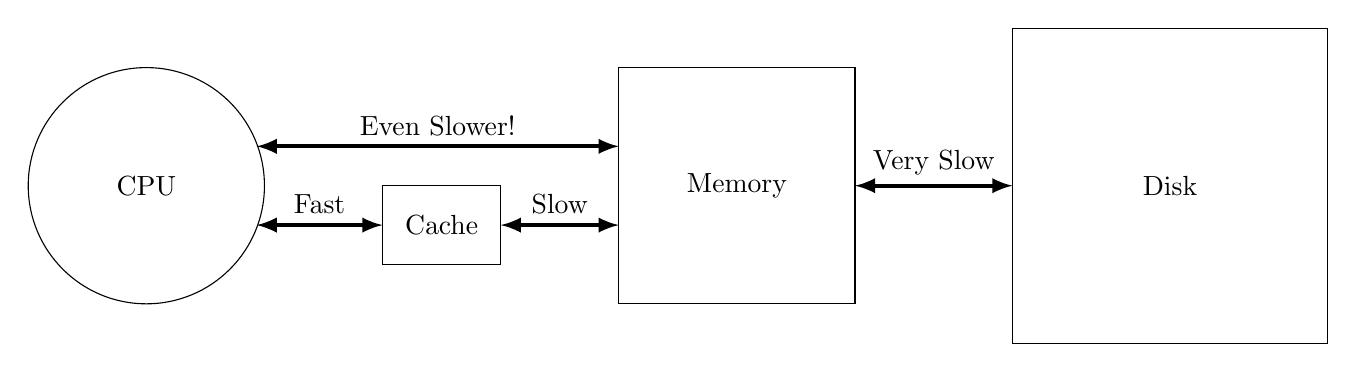
\begin{tikzpicture}
			
			\draw (0,0) circle [radius=1.5] node[midway] {CPU};
			\draw[<->, thick, >=latex, line width=1.5pt] (1.4,-0.5) -- (3,-0.5) node[midway, above] {Fast};
			\draw[<->, thick, >=latex, line width=1.5pt] (1.4,+0.5) -- (6,+0.5) node[midway, above] {Even Slower!};
			
			\draw (3,-1) rectangle (4.5,0) node[midway] {Cache};
			\draw[<->, thick, >=latex, line width=1.5pt] (4.5,-0.5) -- (6,-0.5) node[midway, above] {Slow};
			
			\draw (6,-1.5) rectangle (9,+1.5) node[midway] {Memory};
			\draw[<->, thick, >=latex, line width=1.5pt] (9,0) -- (11,0) node[midway, above] {Very Slow};
			
			\draw (11,-2) rectangle (15,+2) node[midway] {Disk};
			
			
		\end{tikzpicture}
	\end{center}
	
	The CPU acts as the central hub, orchestrating the flow of data between memory, storage, cache, input devices, and output devices as needed to perform tasks and run programs. Data and instructions move between these components through various buses and pathways within the computer system, but these connections are typically abstracted from the user and managed by the computer's hardware and operating system.
	
	\section{Shell Basics on UNIX}
	
	In this section, we will discuss the basics of using the shell in Unix systems, which provide a powerful interface for interacting with the operating system. While Unix serves as the foundation for many operating systems, it is important to distinguish it from Linux, an open-source variant inspired by Unix. macOS, another Unix-based system, shares similarities with both Linux and traditional Unix but incorporates unique features tailored for Apple devices. Despite these differences, the foundational shell commands and scripting principles remain largely consistent across Unix, Linux, and macOS, making these skills highly transferable.
	
	Let's start by creating a new folder (directory) in Linux, the operating system I'm using, via the \codebox{mkdir} command in a terminal.
	
	First, open a terminal application. This step may vary depending on your UNIX/Linux distribution, but typically, you can find the terminal in the Applications menu or by pressing the keyboard shortcut \codebox{Ctrl+Alt+T}.
	
	Next, navigate to the location where you want to create the new folder. You can use the \codebox{cd} command to change directories. For instance, to create the folder in your home directory, type \codebox{cd \textasciitilde}.
	
	Once you're in the desired location, create the folder using the \codebox{mkdir} command followed by the desired folder name. For example, to create a folder named \codebox{Cfolder}, type:
	
	\begin{verbatim}
		mkdir Cfolder
	\end{verbatim}
	
	Finally, press the \codebox{Enter} key to execute the command.
	
	Let's begin by practicing some basic commands:
	
	\textbf{Current directory}: To know your current directory, use the command \codebox{pwd}. It will display the path of the directory you are currently in. To view all the files and folders in the current directory, use the command \codebox{ls}. This will provide a list of all the files and folders. Look for a folder named \codebox{Cfolder} in the list of files and folders (if you have did the previous step successfully!). Once you find it, you'll use the following steps to navigate and work within that folder. To open the \codebox{Cfolder} folder in the file manager, use the command \codebox{open Cfolder}. 
    
    \textbf{Moving back and forth in directories}: To change your current directory to the \codebox{Cfolder} folder, use the command \codebox{cd Cfolder} in the terminal. This command allows you to move into the specified folder (use \codebox{pwd} to double check!) If you want to go back to the initial directory, simply use the command \codebox{cd} without any arguments. This will take you back to the \codebox{/home/username} directory, where \codebox{username} is what you picked during installation of Linux. To go back one folder, use the command \codebox{cd ..}. This will navigate you up one level in the directory structure. 
    
    \textbf{Making a file}: Now, go back to \codebox{Cfolder} directory. If you want to create a text file named "AnneMarie", use the command \codebox{nano AnneMarie.txt}. This will open the file editor where you can write and edit text. To open the \codebox{AnneMarie.txt} file in the Nano text editor, use the command \codebox{nano AnneMarie.txt} again. This allows you to make changes to the file. If you wish to save your changes, press \codebox{Ctrl+O} and then press \codebox{Enter}. This will save the file. Alternatively, if you want to save and exit the Nano text editor, press \codebox{Ctrl+X} and then press \codebox{Enter}. This will save the changes and return you to the terminal. 
    
    To reopen the \codebox{AnneMarie.txt} file in the terminal using the Nano text editor, use the command \codebox{nano AnneMarie.txt}. If you prefer to open the \codebox{AnneMarie.txt} file in the Windows environment, use the command open \codebox{AnneMarie.txt} after saving the file. This will open the file using the default application associated with \codebox{.txt} files.
	
	
	\textbf{Copy and Paste}: To copy the \codebox{AnneMarie.txt} file and paste it into another directory, you can use the \codebox{cp} command, like \codebox{cp AnneMarie.txt /path/to/destination/directory/}. Replace \codebox{/path/to/destination/directory/} with the actual path of the directory where you want to paste the file. 
	
	\textbf{View a file}: The \codebox{cat} command is used to display the contents of a file in the terminal. It can be helpful when you want to quickly view the contents of files. Here's an \codebox{.txt} file example: \codebox{cat AnneMarie.txt}. Running this command will print the contents of \codebox{AnneMarie.txt} in the terminal window. Easier way just double click on the file!
	
	\textbf{Finding a folder or file}: To find a file or folder using the \codebox{locate} command or similar commands, you need to have the appropriate indexing database set up on your system. The \codebox{locate} command searches this database for file and folder names. For example, \codebox{locate AnneMarie.txt}, will search the indexing database for any files or folders with the name \codebox{AnneMarie.txt} and display their paths if found. In this case, nothing is shown in terminal. Since we just made this file, the database including directories is not updated to include this file. To update the directory database in all memory, we have to use the command \codebox{updatedb}, and you will probably get the \codebox{/var/lib/plocate/: Permission denied} message, indicating that you do not have the necessary permissions to access the directory. To solve the issue and update the directories index successfully, use the \codebox{sudo updatedb} which prompts you to a password which you picked. Enter the password, it might not be shown when you are entering the password, then press \codebox{Enter}. By this command, you are running the \codebox{updatedb} with superuser (root) privileges. \codebox{sudo} stands for "Super User Do" and is a command that allows regular users to execute commands with the security privileges of the superuser. Now you can use command \codebox{locate}, but this time it shows the directory that the file is saved. Alternatively, you can use \codebox{find /path/to/search/directory -name AnneMarie.txt}. Replace \codebox{/path/to/search/directory} with the directory where you want to start the search.
	
	
	
	\begin{tcolorbox}[myboxstyle]
		
		{\Large \textbf{\textcolor{cherry}{Tips!}}} Debugging is an essential aspect of programming. No programmer possesses complete knowledge or can remember every command, especially when working with multiple programming languages. However, it is crucial to know where to find the answers. Here are two approaches to tackle a specific issue:
		
		\vspace{\baselineskip}
		
		1. Use internet. For instance, search for "permission denied on Linux." Take a quick look at the top search results, paying particular attention to reputable sources such as \href{https://www.stackoverflow.com}{Stack Overflow}. Spend a few minutes scrolling through the search results. 
		
		\vspace{\baselineskip}
		
		2. Engage with ChatGPT by asking a specific question related to the problem you encountered. For example, you could ask, "I tried \codebox{updatedb} on Linux terminal, and it gives me Permission denied. How can I solve it?"
		
	\end{tcolorbox}
	
	
	\textbf{Remove}: The \codebox{rm} command is used to remove (delete) files and directories. It's important to exercise caution when using this command, as deleted files cannot be easily recovered. Here's an example to remove the \codebox{AnneMarie.txt} file: \codebox{rm AnneMarie.txt}. This command will permanently delete the \codebox{AnneMarie.txt} file. Be sure to double-check the file name and verify that you want to delete it.
	
	The \codebox{rmdir} command is used to remove (delete) empty directories. It cannot remove directories that have any files or subdirectories within them. Here's an example: \codebox{rmdir empty\_directory}. Replace \codebox{empty\_directory} with the name of the directory you want to remove. This command will only work if the directory is empty. If there are any files or subdirectories inside it, you'll need to delete them first or use the \codebox{rm} command with appropriate options to remove them recursively.
	
	Let's checkout some OS and hardware characteristics such as Linux distribution, CPU, disk, and RAM.
	
	\textbf{Linux distribution}: The \codebox{lsb\_release -a} command provides comprehensive information about your Linux distribution, including the release version, codename, distributor ID, and other relevant details. The \codebox{-a} option is a command-line option or flag that stands for "all." When used with the \codebox{lsb\_release} command, it instructs the command to display all available information about the Linux distribution. It is a convenient way to quickly check the specifics of your Linux distribution from the command line. My Linux distribution is:
	
	\begin{lstlisting}
		Distributor ID:	Ubuntu
		Description:	Ubuntu 22.04.2 LTS
		Release:	22.04
		Codename:	jammy
	\end{lstlisting}
	
	
	\textbf{CPU}: The \codebox{lscpu} command is used to gather and display information about the CPU (Central Processing Unit) and its architecture on a Linux system. It provides detailed information about the processor, including its model, architecture, number of cores, clock speed, cache sizes, and other relevant details. \textbf{Some} of details for my system:
	
	\begin{lstlisting}
		Architecture:          x86_64
		  CPU op-mode(s):      32-bit, 64-bit
		  Address sizes:       39 bits physical, 48 bits virtual
		  Byte Order:          Little Endian
		CPU(s):                8
		  On-line CPU(s) list: 0-7
		Vendor ID:             GenuineIntel
		  Model name:          Intel(R) Core(TM) i7-7700HQ CPU @ 2.80GHz
		  CPU family:          6
		  Model:               158
		  Thread(s) per core:  2
	\end{lstlisting}
	
	\textbf{Disk space available}: The \codebox{df -h} command is used to display information about the disk space usage on your Linux system. In this command, \codebox{df} stands for \textbf{disk free}, and \codebox{-h} is a command-line option or flag that stands for \textbf{human-readable}. The
	
	\begin{lstlisting}
		Filesystem      Size  Used Avail Use% Mounted on
		/dev/sda2       228G  113G  104G  53% /
	\end{lstlisting}
	
	\codebox{/dev/sda2} is a partition identifier that represents the second partition on the first SATA (or SCSI) disk (sda). It typically contains the main file system of your Linux system. The actual partition identifiers may differ depending on your system's configuration and the number of disks or partitions present.
	
	\textbf{Information about the RAM}: In the command \codebox{free -h}, \codebox{free} represents the command used to display memory usage statistics, and \codebox{-h} is a command-line option that stands for \textbf{human-readable}.
	
	\begin{lstlisting}
		          total   used    free    shared  buff/cache  available
		Mem:      15Gi    4.4Gi   3.3Gi   637Mi   7.8Gi       10Gi
		Swap:     2.0Gi   0B      2.0Gi
		
	\end{lstlisting}

    The \textbf{Swap} space is a portion of the hard drive that is used as virtual memory by the operating system. It acts as an extension to the physical memory (RAM) and allows the system to temporarily store data that doesn't fit into the RAM.
	
	
	\textbf{Short keys in terminal}: \codebox{Ctrl+L} to remove the history of terminal. Pressing Up Arrow Key will show you the previous commands. To copy from terminal you have to press \codebox{Cntrl + Shift + C} and to paste a command press \codebox{Ctrl + shift + V}. 
	
	
	\section*{Supplementary Material}
	
	Linux provides a variety of command-line utilities for tasks ranging from file management to system monitoring and networking. Below is a categorized list of commonly used Linux terminal commands.
	
	
	
	
	\begin{itemize}
		\item \textbf{File and Directory Management}
			\begin{itemize}
				\item \textbf{\texttt{ls}}: Lists directory contents.
				\begin{itemize}
					\item Example: \texttt{ls -l} (detailed listing)
				\end{itemize}
				\item \textbf{\texttt{cd}}: Changes the current directory.
				\begin{itemize}
					\item Example: \texttt{cd /home/user/}
				\end{itemize}
				\item \textbf{\texttt{pwd}}: Prints the current working directory.
				\item \textbf{\texttt{mkdir}}: Creates a new directory.
				\begin{itemize}
					\item Example: \texttt{mkdir new\_folder}
				\end{itemize}
				\item \textbf{\texttt{rmdir}}: Removes an empty directory.
				\begin{itemize}
					\item Example: \texttt{rmdir old\_folder}
				\end{itemize}
				\item \textbf{\texttt{rm}}: Removes files or directories.
				\begin{itemize}
					\item Example: \texttt{rm file.txt}, \texttt{rm -r folder\_name}
				\end{itemize}
				\item \textbf{\texttt{cp}}: Copies files and directories.
				\begin{itemize}
					\item Example: \texttt{cp source.txt destination.txt}
				\end{itemize}
				\item \textbf{\texttt{mv}}: Moves or renames files and directories.
				\begin{itemize}
					\item Example: \texttt{mv file.txt new\_location/}
				\end{itemize}
				\item \textbf{\texttt{touch}}: Creates an empty file.
				\begin{itemize}
					\item Example: \texttt{touch newfile.txt}
				\end{itemize}
				\item \textbf{\texttt{find}}: Searches for files in a directory hierarchy.
				\begin{itemize}
					\item Example: \texttt{find /path -name "file.txt"}
				\end{itemize}
				\item \textbf{\texttt{stat}}: Displays detailed information about a file.
			\end{itemize}
		
		\item \textbf{Viewing and Editing Files}
			\begin{itemize}
				\item \textbf{\texttt{cat}}: Displays file contents.
				\begin{itemize}
					\item Example: \texttt{cat file.txt}
				\end{itemize}
				\item \textbf{\texttt{more}}: Views file content one screen at a time.
				\item \textbf{\texttt{less}}: Similar to \texttt{more} but allows backward navigation.
				\item \textbf{\texttt{nano}}, \textbf{\texttt{vi}}, \textbf{\texttt{vim}}: Text editors for editing files.
				\begin{itemize}
					\item Example: \texttt{nano file.txt}
				\end{itemize}
				\item \textbf{\texttt{head}}: Displays the first lines of a file.
				\begin{itemize}
					\item Example: \texttt{head -n 10 file.txt}
				\end{itemize}
				\item \textbf{\texttt{tail}}: Displays the last lines of a file.
				\begin{itemize}
					\item Example: \texttt{tail -f log.txt}
				\end{itemize}
			\end{itemize}
		
		\item \textbf{Permissions and Ownership}
			\begin{itemize}
				\item \textbf{\texttt{chmod}}: Changes file permissions.
				\begin{itemize}
					\item Example: \texttt{chmod 755 file.sh}
				\end{itemize}
				\item \textbf{\texttt{chown}}: Changes file ownership.
				\begin{itemize}
					\item Example: \texttt{chown user:group file.txt}
				\end{itemize}
			\end{itemize}
		
		\item \textbf{System Information and Monitoring}
			\begin{itemize}
				\item \textbf{\texttt{uname}}: Shows system information.
				\begin{itemize}
					\item Example: \texttt{uname -a}
				\end{itemize}
				\item \textbf{\texttt{df}}: Displays disk space usage.
				\begin{itemize}
					\item Example: \texttt{df -h}
				\end{itemize}
				\item \textbf{\texttt{du}}: Shows disk usage of files and directories.
				\begin{itemize}
					\item Example: \texttt{du -sh folder/}
				\end{itemize}
				\item \textbf{\texttt{top}}: Displays real-time system processes.
				\item \textbf{\texttt{htop}}: Enhanced version of \texttt{top} (requires installation).
				\item \textbf{\texttt{free}}: Shows memory usage.
				\begin{itemize}
					\item Example: \texttt{free -h}
				\end{itemize}
				\item \textbf{\texttt{uptime}}: Displays system uptime.
				\item \textbf{\texttt{who}}: Shows who is logged in.
			\end{itemize}
		
		\item \textbf{Process Management}
			\begin{itemize}
				\item \textbf{\texttt{ps}}: Lists running processes.
				\begin{itemize}
					\item Example: \texttt{ps aux}
				\end{itemize}
				\item \textbf{\texttt{kill}}: Terminates a process by PID.
				\begin{itemize}
					\item Example: \texttt{kill 1234}
				\end{itemize}
				\item \textbf{\texttt{killall}}: Terminates all processes by name.
				\begin{itemize}
					\item Example: \texttt{killall firefox}
				\end{itemize}
				\item \textbf{\texttt{jobs}}: Lists background jobs.
				\item \textbf{\texttt{bg}}/\textbf{\texttt{fg}}: Resumes background jobs in the background/foreground.
			\end{itemize}
		
		\item \textbf{Networking}
			\begin{itemize}
				\item \textbf{\texttt{ping}}: Checks network connectivity to a host.
				\begin{itemize}
					\item Example: \texttt{ping google.com}
				\end{itemize}
				\item \textbf{\texttt{curl}}: Fetches content from a URL.
				\begin{itemize}
					\item Example: \texttt{curl http://example.com}
				\end{itemize}
				\item \textbf{\texttt{wget}}: Downloads files from a URL.
				\item \textbf{\texttt{ifconfig}}/\textbf{\texttt{ip}}: Shows or configures network interfaces.
				\begin{itemize}
					\item Example: \texttt{ip a}
				\end{itemize}
				\item \textbf{\texttt{netstat}}/\textbf{\texttt{ss}}: Displays network connections.
				\item \textbf{\texttt{scp}}: Securely copies files between hosts.
				\begin{itemize}
					\item Example: \texttt{scp file.txt user@remote:/path/}
				\end{itemize}
			\end{itemize}
		
		\item \textbf{Compression and Archiving}
			\begin{itemize}
				\item \textbf{\texttt{tar}}: Archives files.
				\begin{itemize}
					\item Example: \texttt{tar -cvf archive.tar file/}
				\end{itemize}
				\item \textbf{\texttt{gzip}}/\textbf{\texttt{gunzip}}: Compresses/Decompresses files.
				\begin{itemize}
					\item Example: \texttt{gzip file.txt}
				\end{itemize}
				\item \textbf{\texttt{zip}}/\textbf{\texttt{unzip}}: Creates/extracts ZIP archives.
				\begin{itemize}
					\item Example: \texttt{zip archive.zip file/}
				\end{itemize}
			\end{itemize}
		
		\item \textbf{Package Management}
			\begin{itemize}
				\item \textbf{\texttt{apt}} (Debian/Ubuntu): Manages software packages.
				\begin{itemize}
					\item Example: \texttt{sudo apt update \&\& sudo apt upgrade}
				\end{itemize}
				\item \textbf{\texttt{yum}}/\textbf{\texttt{dnf}} (RHEL/Fedora): Manages software packages.
				\item \textbf{\texttt{pacman}} (Arch): Manages software packages.
				\begin{itemize}
					\item Example: \texttt{sudo pacman -Syu}
				\end{itemize}
			\end{itemize}
		
		\item \textbf{Miscellaneous}
			\begin{itemize}
				\item \textbf{\texttt{echo}}: Prints text to the terminal.
				\begin{itemize}
					\item Example: \texttt{echo "Hello, World!"}
				\end{itemize}
				\item \textbf{\texttt{date}}: Displays the current date and time.
				\item \textbf{\texttt{man}}: Opens the manual for a command.
				\begin{itemize}
					\item Example: \texttt{man ls}
				\end{itemize}
				\item \textbf{\texttt{alias}}: Creates command shortcuts.
				\begin{itemize}
					\item Example: \texttt{alias ll="ls -la"}
				\end{itemize}
				\item \textbf{\texttt{history}}: Shows the command history.
				\item \textbf{\texttt{clear}}: Clears the terminal screen.
			\end{itemize}
		
	\end{itemize}
	
	In this section, we have covered only the basics of using the shell, providing a foundation for understanding command-line interactions. For those interested in exploring more, Linux users can refer to the \href{https://ubuntu.com/tutorials/command-line-for-beginners#1-overview}{Ubuntu website} and its "Command Line for Beginners" tutorial. Mac users can consult \href{https://support.apple.com/en-ca/guide/terminal/apd53500956-7c5b-496b-a362-2845f2aab4bc/mac}{Apple's official website} for guidance, specifically the "Intro to Shell Scripts in Terminal on Mac" section. These resources offer a more comprehensive overview and step-by-step guidance to enhance your shell proficiency.
	
	
	
	
	

	
	\chapter{Fundamentals of C Language}
	
	\section*{Introduction}
	
	This chapter is designed to provide an introduction to fundamental concepts in C, including data types, variables, and control flow statements such as if and loops. Some of students with prior knowledge of programming might already know these concepts, but we will delve into each topic extensively and provide detailed explanations. Our goal is to ensure that everyone, regardless of their programming background, can grasp these essential concepts effectively. We will illustrate each concept with practical examples and problem-solving exercises to enhance understanding, as these concepts form the backbone of C programming.
	
	
	\section{Your First C Program: \codebox{Hello, McMaster!}}
	
	In this section, we will guide you through the process of writing, understanding, and running your first C program. The upcoming subsections are designed to introduce you to the fundamental concepts of C programming. First, in \hyperref[sub:UCPSFM]{\textcolor{orange!80!black}{Understanding C Program Structure and File Management}}, you'll learn how to create and manage a C file, explore the general structure of a C program, and familiarize yourself with essential tools like text editors and IDEs. Then, in \hyperref[sub:FS]{\textcolor{orange!80!black}{From Source Code to Execution: Compiling and Running}}, we’ll walk you through the steps to transform your written code into an executable program, covering the compilation process, error handling, and how to execute your program successfully. By the end of this section, you’ll not only have a working program but also a solid grasp of the core C programming workflow.
	
	
	
	
	
	
	\subsection{Understanding C Program Structure and File Management}\label{sub:UCPSFM}
	
	Let's make a new file using \codebox{nano Hello.c} where the \textbf{.c} extension represent a C file. Before closing the the opened file in terminal copy and paste the following code in the file and save it. To paste the the copied section you have to use \codebox{Ctrl + shift + V}. Press \codebox{Ctrl + X} then \codebox{y} and press Enter to save before exit.
	
	\begin{lstlisting}
		// this code is written by Pedram
		#include <stdio.h>
		
		// the main function
		int main(void) {
			/* calling "printf" function
			the "defination" is included in "stdio" library */
			printf("Hello, McMaster!\n");
		}
	\end{lstlisting}
	
	Open the file by \codebox{open Hello.c}. This is a more user friendly environment to edit the code. Maybe the main difference is I can click different parts of the code and edit the code. During you lab lectures this week, you TAs will discuss Visual Studio Code IDE (Integrated Development Environment) which support many programming languages, including C, as well as many useful tools such as automatic code formatting. I strongly suggest to install it and set it up for C format for the next lectures. If I want to modify the code in terms of extra spaces in the code using \codebox{open Hello.c} it will take me some time. But if you have Visual Studio Code installed, in the terminal enter \codebox{code Hello.c} to open the same code in Visual Studio Code (VSC).Right click on the code and choose \textbf{Format Document} which automatically modifies the code in C format.
	
	\begin{tcolorbox}[myboxstyle]
		{\Large \textbf{\textcolor{cherry}{Tips!}}} Get your hands dirty! I promise you that by only reading these notes you will NOT be able to learn programming. You have to write, modify, and change every code in these notes. Play with them like you play video games!
		
	\end{tcolorbox}
	
    Anything starts with two slashes, \codebox{//}, until the end of the line is a comment and it will not be executed. To make multiple lines as comments, you can place them between \codebox{/*} and \codebox{*/}. The following lines in the code are all comments:
    
    \begin{lstlisting}
    	// this code is written by Pedram
    	
    	// the main function
    	
    	/* calling "printf" function
    	the "defination" is included in "stdio" library */
    \end{lstlisting}

    Based on the IDE that you are using the colour of the comments might be different. I have said earlier that understanding C codes especially written by someone else might be difficult. Comments are supposed to be helpful to remember or tell others what is the purpose of each part of the code or even how it works.
    
    So the first line which is really executed is \codebox{include <stdio.h>}. Usually at the beginning of a code, we include libraries used in the code. \codebox{include <stdio.h>} tells C to read \textbf{header file} named \codebox{stdio} with extension \codebox{.h} which stands for \textbf{header file}. In this library the definition of function \codebox{printf} is mentioned. Any time you forget what library a function is in, you can ask your best friend \textbf{Google} or \textbf{ChatGPT} by simply asking "\href{https://www.google.com/search?channel=fs&client=ubuntu-sn&q=what+library+in+C+printf+is+in}{what library in C printf is in}."
    
    The second line that will be executed is \codebox{int main(void)} as a function. In C, defining a function starts with the type of value the function returns, which in this case it is \codebox{int}. The \codebox{int} means \textbf{integer} and the function \codebox{main} will automatically return the value \textbf{0} if there is no error in the code.
    
    The \codebox{main} is the name of function. This function must be included in all C programs, and you have to write your code inside this function.
    
    Between the parentheses, \codebox{void} what inputs your program needs and requires the user to give the input(s) every time the code is going to be executed. In this case, we don't have any input so it is \codebox{void}, or we can define \codebox{int main()} instead of \codebox{int main(void)}. Both means the program requires no input(s).
    
    Anything between \codebox{\{}, right after \codebox{int main(void)}, and \codebox{\}}, at the end of the code, is called \textbf{compound statement} or \textbf{code block}, which belongs to \codebox{main} function. So the following statement is the general format that we have to include in all C programs:
    
    \begin{lstlisting}
    	Inclduing Library
    	
    	int main(){
    	
    	your statements
    	
        }
    \end{lstlisting}
    
    In this code, \codebox{printf("Hello, McMaster!\textbackslash n")} is the only statement we have and \codebox{printf} function is used to print a text. Between \codebox{(} and \codebox{)} the arguments for the function \codebox{printf} is given, which is a string or text to be printed!
    
    A string is sequence of characters enclosed within quotation marks. \codebox{"Hello, McMaster!\textbackslash n"} is the string that will be printed. The backslash \codebox{\textbackslash} before \codebox{n} tells C to go to (\textbf{n})ext line after printing \codebox{Hello, McMaster!}. Try to compile and run the code two times with \codebox{\textbackslash n} and two times without \codebox{\textbackslash n} and see the difference in the terminal! At the end of this line there is \codebox{;} indicating the command for this line has ended. A reminder, the closing bracket \codebox{\}} at the end, means the end of function \codebox{main}!
	
	\subsection{From Source Code to Execution: Compiling and Running}\label{sub:FS}
	
	Now we have to convert the program, the file \codebox{Hello.c}, to a format that machine can understand and execute. It usually involves, \textbf{Pre-processing}, \textbf{Compiling}, and \textbf{Linking}. During \textbf{Pre-processing} some modification will be done automatically to the code, before making the executable \textbf{object} code in \textbf{Compiling} step. These two steps are done at the same time and automatically, so won't need to be worried about it! In the Linking step, the library included will be linked to the executable file. Since this code is using a standard library, \codebox{<stdio.h>}, it happens automatically. Again, you don't need to be worried!!!
	
	To compile the program in UNIX based OS, usually \codebox{cc} is used. Open a terminal in the directory where \codebox{Hello.c} file is located (please refer to the section Shell Basics on Linux). Type \codebox{cc Hello.c}. Check out the directory. A new executable \textbf{object} file named \codebox{a.out} by default will be created.
	
	If you see the following error after executing \codebox{cc Hello.c}, it means you are not in the same directory where \codebox{Hello.c} is located. A reminder, use \codebox{pwd} to check your current directory.
	
	\begin{lstlisting}
		cc1: fatal error: Hello.c: No such file or directory
		compilation terminated.
	\end{lstlisting}
	
	
    \begin{tcolorbox}[myboxstyle]
    	{\Large \textbf{\textcolor{cherry}{Visual Studio Code!}}} You may open the code in Visual Studio Code (VSCode) by running \codebox{code Hello.c} in the terminal. Again make sure current directory is where \codebox{Hello.c} is located, otherwise you will see an error indicating the is no such a file in this directory. At the top of VSCode opened, press \textbf{View} and click \textbf{Terminal}. A window will be opened at the bottom, named \textbf{TERMINAL}. There is no difference between this Terminal and terminal you open using \codebox{Ctrl + Alt + T}. Make sure the directory of this Terminal in VScode is the where \codebox{Hello.c} is located to avoid the error I have mention before running \codebox{cc Hello.c} in the terminal.
    	
    	After \codebox{cc Hello.c} if there is no problem, you should be able to see a new executable \textbf{object} file named \codebox{a.out} by default in the directory.
    \end{tcolorbox}
    
    At this stage the code is compiled, the \textbf{object} \codebox{a.out} readable by machine is created. This means the program is translated to a language that machine can understand and it saved in the \textbf{object} file \codebox{a.out}. Now it is time to tell the machine to run the translated code and show us the result. Run \codebox{./a.out} in the terminal. Again, make sure you are in the directory where \codebox{a.out} is located. It is done! you should be able to see the result!
    
    \textcolor{cherry}{\textbf{{\large Hello, McMaster!}}}
    
    I have mentioned the name \codebox{a.out} is given to the \textbf{object} file by default. I can define any name I want. Lets remove the previous object file by \codebox{rm a.out} and make a new one with the name "\textbf{Brad}" by using \codebox{cc -o Brad Hello.c}. The compiler \codebox{cc} has many options, and \codebox{-o} means translate the program \codebox{Hello.c} to the machine language with an (\textbf{o})bject file named \codebox{Brad}. Now you must be able to see an \textbf{object} file named \codebox{Brad} in the same directory. If you run the command line \codebox{./Brad} in the same directory, you should be able to see the output.
    
    \begin{tcolorbox}[myboxstyle]
    	
    	{\Large \textbf{\textcolor{cherry}{GCC compiler}}} Another popular compiler in C is GCC (GNU Compiler Collection) compiler supported by Unix OS. It is known for its robustness, efficiency, and compatibility with multiple platforms. GCC supports various optimizations and provides comprehensive error checking, making it a reliable choice for compiling C code.
    	
    	One notable feature of GCC is its similarity to the "cc" compiler command. This similarity stems from the fact that on many Unix-like systems, the "cc" command is often a symbolic link or an alias for GCC. Therefore, using "cc" to compile your code essentially invokes the GCC compiler with its default settings. GCC offers numerous options to control various aspects of the compilation process, such as optimization levels, debugging symbols, and specific target architectures.
    	
    	You can compile the same program using GCC instead of \codebox{cc} by executing \codebox{gcc -o Brad Hello.c} in the terminal.
    	
    \end{tcolorbox}

    The \textbf{object} file \codebox{./Brad} is executable in any Unix based OS. It is software of application you developed!
    
	\section{Integer Data Type}
	
	In contemporary C compilers, there is support for a range of integer sizes spanning from 8 to 64 bits. However, it is worth noting that the specific names assigned to each size of integer may differ among different compilers, leading to potential confusion among developers. First we need to know how data is stored in computers.
	
	\subsection{Binary Representation}
	
	In the world of computers, information is stored and processed as sequences of bits, representing either a 0 or a 1. This fundamental concept forms the basis of how data is handled by computer systems. Consider the scenario where we have a fixed number of bits, denoted by N, to represent our numbers. Let's take \textbf{N=4} to save an \codebox{int} number where \codebox{int} in C stands for \textbf{integer} number. In this case, we are allocating nine bits to express our numerical values. If the integer is \codebox{unsigned} then:
	
	
	\begin{itemize}
		
		\setlength{\itemsep}{-5pt}
		\item 0  = 0000
		\item 1  = 0001
		\item 2  = 0010
		\item 3  = 0011
		\item 4  = 0100
		\item 5  = 0101
		\item 6  = 0110
		\item 7  = 0111
		\item 8  = 1000
		\item 9  = 1001
		\item 10 = 1010
		\item 11 = 1011
		\item 12 = 1100
		\item 13 = 1101
		\item 14 = 1110
		\item 15 = 1111 = $2^N-1$
		
	\end{itemize}
	
	\begin{tcolorbox}[myboxstyle]
		
		{\Large \textbf{\textcolor{cherry}{More example?!}}} If N = 3 then for \codebox{unsigned} integer we would have:
		\begin{itemize}
			
			\setlength{\itemsep}{-5pt}
			
			\item 0 = 000
			\item 1 = 001
			\item 2 = 010
			\item 3 = 011
			\item 4 = 100
			\item 5 = 101
			\item 6 = 110
			\item 7 = 111 = $2^N-1$
			
		\end{itemize}
	\end{tcolorbox}

    \noindent which means the range of numbers can be saved as \codebox{unsigned} integer in C is from $0$ to $2^{N}-1$. For \codebox{signed} integers, the negative numbers can be obtained by inverting the bits then adding one to the result. This method is called the two's complement operation.
	
	\begin{itemize}
		
		\setlength{\itemsep}{-5pt}
		
		\item \textbf{-8 = 1000} = $-2^{N-1}$
		\item -7 = (inverting 0111, we have 1000, +1 is:)1001
		\item -6 = (inverting 0110, we have 1001, +1 is:)1010
		\item -5 = (inverting 0101, we have 1010, +1 is:)1011
		\item -4 = (inverting 0100, we have 1011, +1 is:)1100
		\item -3 = (inverting 0011, we have 1100, +1 is:)1101
		\item -2 = (inverting 0010, we have 1101, +1 is:)1110
		\item -1 = (inverting 0001, we have 1110, +1 is:)1111
		\item 0 = 0000
		\item 1 = 0001
		\item 2 = 0010
		\item 3 = 0011
		\item 4 = 0100
		\item 5 = 0101
		\item 6 = 0110
		\item 7 = 0111 = $2^{N-1}-1$
	\end{itemize}

	Probably you have noticed that 1000 is assigned to -8. In total with 4 bits, a machine can have a combination of $2^4$ zero and ones. It can be seen that all positive numbers starts with 0, and negative ones start with one. Therefore, it is accepted to sign 1000 bit sequence to the lowest number, -8. The range of numbers can be saved as \codebox{signed} integer in C is from $-2^{N-1}$ to $2^{N-1}-1$. Exceeding this range can cause errors, probably unseen, which it is called \textbf{integer overflow}.
	
	\begin{tcolorbox}[myboxstyle]
		
		{\Large \textbf{\textcolor{cherry}{More example?!}}} If N = 3 then for \codebox{unsigned} integer we would have:
		\begin{itemize}
			
			\setlength{\itemsep}{-5pt}
			
			\item \textbf{-4 = 100} = $-2^{N-1}$
			\item -3 = (inverting 011, we have 100, +1 is:)101
			\item -2 = (inverting 010, we have 101, +1 is:)110
			\item -1 = (inverting 001, we have 110, +1 is:)111
			\item 0 = 000
			\item 1 = 001
			\item 2 = 010
			\item 3 = 011 = $2^{N-1}-1$
			
		\end{itemize}
	\end{tcolorbox}

	
	\subsection{Using \codebox{printf} and \codebox{limits.h} to Get the Limits of Integers}\label{subsec:Get integer limits}
	
	Let's see some of these limits using \codebox{limits.h} library. Make a new file using \codebox{nano limit.c} which \codebox{limit} is the name of program given by you, and \codebox{.c} is the extension which stands for C files. Copy and past the following code. Press \codebox{Ctrl + X} then \codebox{y} and Enter to save and close the file. Open the code in VScode, if you have it as IDE, by entering \codebox{code limit.c} in your terminal. Make sure you are in the same directory where you made this file.
	
	\begin{lstlisting}
		// This code is written by ChatGPT
		#include <stdio.h>
		#include <limits.h>
		
		int main() {
			
			printf("Size of char: %zu bits\n", 8 * sizeof(char));
			printf("Signed char range: %d to %d\n", SCHAR_MIN, SCHAR_MAX);
			printf("Unsigned char range: %u to %u\n", 0, UCHAR_MAX);
			printf("\n");
			
			printf("Size of short: %zu bits\n", 8 * sizeof(short));
			printf("Signed short range: %d to %d\n", SHRT_MIN, SHRT_MAX);
			printf("Unsigned short range: %u to %u\n", 0, USHRT_MAX);
			printf("\n");
			
			printf("Size of int: %zu bits\n", 8 * sizeof(int));
			printf("Signed int range: %d to %d\n", INT_MIN, INT_MAX);
			printf("Unsigned int range: %u to %u\n", 0, UINT_MAX);
			printf("\n");
			
			printf("Size of long: %zu bits\n", 8 * sizeof(long));
			printf("Signed long range: %ld to %ld\n", LONG_MIN, LONG_MAX);
			printf("Unsigned long range: %u to %lu\n", 0, ULONG_MAX); // change %u to lu
			printf("\n");
			
			printf("Size of long long: %zu bits\n", 8 * sizeof(long long));
			printf("Signed long long range: %lld to %lld\n", LLONG_MIN, LLONG_MAX);
			printf("Unsigned long long range: %u to %llu\n", 0, ULLONG_MAX); // change %u to llu
		}
	\end{lstlisting}
	
	Let's check the code line-by-line. 
	
    \textbf{1.} \codebox{\#include <limits.h>}: This is a preprocessor directive that includes the header file \codebox{limits.h} in the C program. The \codebox{limits.h} header provides constants and limits for various data types in the C language, such as the minimum and maximum values that can be represented by different types.
	
	\textbf{2.} Placeholders: is a special character or sequence of characters that is used within a formatted string to represent a value that will be substituted during runtime. Placeholders are typically used in functions like \codebox{printf} or \codebox{sprintf} to dynamically insert values into a formatted output. When the program runs, the placeholders are replaced with the actual values passed as arguments to the formatting function. The values are appropriately converted to match the format specifier specified by the corresponding placeholders. Placeholders provide a flexible way to format output by allowing dynamic insertion of values. They help in producing formatted and readable output based on the specified format specifiers and the provided values.
	
	\begin{itemize}
		\item \codebox{\%zu}: This is a placeholder used with \codebox{printf} to print the value of an \codebox{unsigned} \textbf{integer}.
		\item \codebox{\%d}: This is a placeholder used to \codebox{printf} the value of a \codebox{signed integer}.
		\item \codebox{\%u}: This is a placeholder used to \codebox{printf} the value of an \codebox{unsigned} \textbf{integer}.
		\item \codebox{\%ld}: This is a placeholder used to \codebox{printf} the value of a \codebox{signed long} \textbf{integer}.
		\item \codebox{\%lu}: This is a placeholder used to \codebox{printf} the value of an \codebox{unsigned long} \textbf{integer}.
		\item \codebox{\%lld}: This is a placeholder used to \codebox{printf} the value of a \codebox{signed long long} \textbf{integer}.
		\item \codebox{\%llu}: This is a placeholder used to \codebox{printf} the value of an \codebox{unsigned long long} \textbf{integer}.
	\end{itemize}
	

	
	\textbf{3.} \codebox{sizeof()}: This is an operator in C that returns the size of a variable or a data type in bytes. In the given code, \codebox{sizeof()} is used to determine the size of different data types (e.g., char, int, long, long long). The result of \codebox{sizeof()} is then multiplied by 8 to obtain the size in bits.
	
	\textbf{4.} \codebox{printf("\textbackslash n")}: This line of code is using \codebox{printf} to print a newline character \codebox{\textbackslash n}. It adds a line break, resulting in a new line being displayed in the console output.
	
	\textbf{5.} \codebox{NAME\_MIN} and \codebox{NAME\_MAX}: The code refers to variables like \codebox{SCHAR\_MIN}, \codebox{SCHAR\_MAX}, \codebox{INT\_MIN}, \codebox{INT\_MAX}, etc. These variables are predefined in the C library, specifically in the limits.h header file. They represent the minimum and maximum values that can be stored in the respective data types (e.g., \codebox{char}, \codebox{int}, \codebox{short}, \codebox{long}, \codebox{long long}).
	
	\textbf{6.} \codebox{char}, \codebox{int}, \codebox{short}, \codebox{long}, and l\codebox{long long}: These are data types in the C language. They represent different ranges of integer values that can be stored. The code provided displays the size and range of each of these data types, both signed and unsigned.
	
	This time we compile the code with options \codebox{gcc -Wall -W -std=c99 -o limit limit.c} which: 
	
	
	\codebox{-Wall}: This flag enables a set of warning options, known as "\textbf{all warnings}." It instructs the compiler to enable a comprehensive set of warning messages during the compilation process. These warnings help identify potential issues in the code, such as uninitialized variables, unused variables, type mismatches, and other common programming mistakes. By enabling \codebox{-Wall}, you can ensure that a wide range of warnings is reported, assisting in the production of cleaner and more reliable code.
	
	\codebox{-W}: This flag is used to enable additional warning options beyond those covered by \codebox{-Wall}. It allows you to specify specific warning options individually. Without any specific options following \codebox{-W}, it enables a set of commonly used warnings similar to \codebox{-Wall}. By using \codebox{-W}, you have more control over the warning messages generated by the compiler.
	
	\codebox{-std=c99}: This flag sets the C language standard that the compiler should adhere to. In this case, c99 indicates the \textbf{C99 standard}. The \textbf{C99 standard} refers to the ISO/IEC 9899:1999 standard for the C programming language. It introduces several new features and improvements compared to earlier versions of the C standard, such as support for variable declarations anywhere in a block, support for \codebox{//} single-line comments, and new data types like \codebox{long long}. By specifying \codebox{-std=c99}, you ensure that the compiler follows the \textbf{C99 standard} while compiling your code.
	
	\codebox{-o limit}: This flag is used to specify the output file name. In this case, it sets the output file name as "limit". The compiled binary or executable will be named "limit" as a result.
	
	\codebox{limit.c}: This is the source file that contains the C code to be compiled.
	
	After compiling the code, I can run the object file \codebox{limit} in the current directory by \codebox{./limit}. This is the result I get in \textbf{my computer}!
	
	\begin{tcolorbox}[myboxstyleTerminal]
		\begin{verbatim}
			Size of char: 8 bits
			Signed char range: -128 to 127
			Unsigned char range: 0 to 255
			
			Size of short: 16 bits
			Signed short range: -32768 to 32767
			Unsigned short range: 0 to 65535
			
			Size of int: 32 bits
			Signed int range: -2147483648 to 2147483647
			Unsigned int range: 0 to 4294967295
			
			Size of long: 64 bits
			Signed long range: -9223372036854775808 to 9223372036854775807
			Unsigned long range: 0 to 18446744073709551615
			
			Size of long long: 64 bits
			Signed long long range: -9223372036854775808 to 9223372036854775807
			Unsigned long long range: 0 to 18446744073709551615
		\end{verbatim}
	\end{tcolorbox}

    We will find out about the importance of knowing limits in section \hyperref[subsec:A Simple Example for Integer Overflows]{\textcolor{orange!80!black}{A Simple Example for Integer Overflows}}.
	
	\subsection{Declaring and Naming with and without Initializing} \label{sec:declaring}
	
	To declare a variable you can simply use the following format. \codebox{int} is the type of variable and \codebox{Pedram} is the name of variable. You can after this line of code calculate the value of \codebox{Pedram}. 
	
	\begin{lstlisting}
		int Pedram;
	\end{lstlisting}
	
	You may also declare the value for this variable when it is initialized with a value:
	
	\begin{lstlisting}
		int Pedram = 10;
	\end{lstlisting}
     
     
    \begin{tcolorbox}[myboxstyle]
     	
     	{\Large \textbf{\textcolor{cherry}{Tips!}}} There are some reserved names that you cannot use for your variables, including:
     	
     	\codebox{auto}, \codebox{break}, \codebox{case}, \codebox{char}, \codebox{const}, \codebox{continue}, \codebox{default}, \codebox{do}, \codebox{double}, \codebox{else}, \codebox{enum}, \codebox{extern}, \codebox{float}, \codebox{for}, \codebox{goto}, \codebox{if}, \codebox{inline}, \codebox{int}, \codebox{long}, \codebox{register}, \codebox{restrict}, \codebox{return}, \codebox{short}, \codebox{signed}, \codebox{sizeof}, \codebox{static}, \codebox{struct}, \codebox{switch}, \codebox{typedef}, \codebox{union}, \codebox{unsigned}, \codebox{void}, \codebox{volatile}, \codebox{while}, \codebox{\_Bool}, \codebox{\_Complex}, \codebox{\_Imaginary}, \codebox{\#define}, \codebox{\#include}, \codebox{\#undef}, \codebox{\#ifdef}, \codebox{\#endif}, \codebox{\#ifndef}, \codebox{\#if}, \codebox{\#else}, \codebox{\#elif}, \codebox{\#pragma},  and more! Don't worry if you use these you will see some errors and warnings when compiling the the code!
     	
    \end{tcolorbox}


    \begin{tcolorbox}[myboxstyle]
    	
    	{\Large \textbf{\textcolor{cherry}{More Tips!}}} About naming style, if you use only characters like \codebox{a,b,c, ..., z}, no one can follow your code or what is the purpose of this variable. So:
    	\begin{itemize}
    		\item Use meaningful and descriptive names that convey the purpose or nature of the variable. for example, \codebox{rectangle\_height} and \codebox{triangle\_width}
    		\item Avoid excessively long names, but provide enough clarity to understand the purpose of the variable.
    		\item Follow a consistent naming convention, such as \codebox{camelCase} or \codebox{snake\_case}.
    		\item use comments if necessary to explain the purpose or usage of a variable.
    	\end{itemize}
    	
    \end{tcolorbox}

    You can also compile the code with \codebox{-Wextra} flag detecting uninitialized variables. Let's try the following code with and without.
    
    \begin{lstlisting}
    	#include <stdio.h>
    	
    	int main() {
    		int x;
    		int y = x + 5;  // Using uninitialized variable x
    		printf("%d\n", y);
    	}
    \end{lstlisting}

    Compiling the code with \codebox{gcc -o Pedram Pedram.c}, then executing the program with \codebox{./Pedram}. I get the following result:
    
    \begin{lstlisting}
    	-1240674203
    \end{lstlisting}

    If I execute the code one more time, \codebox{./Pedram}, without compiling the code, I get: 
    
    \begin{lstlisting}
    	233918565
    \end{lstlisting}

    \textbf{What is going on????} When you run this code, you may get different output each time because the value of x is unspecified and can contain any arbitrary value. The variable x could be storing whatever value was previously in that memory location, and performing calculations with such a value can lead to unexpected results.
    
    Let's compile the code but this time with \codebox{gcc -Wextra -o Pedram Pedram.c}. In my terminal it tells me \codebox{Using uninitialized variable x} and mentioning the line of code this issue is happening. At this point, the source code \codebox{Pedram.c} is compiled and the Pedram object is available. It means I can execute the program, but I am aware of the fact that this will result a wrong and an unexpected result. There are some warning you have to take serious even more than error! I could see the same warning by compiling the code using \codebox{gcc -Wall -W -std=c99 -o Pedram Pedram.c}
	
	\subsection{Constant Variables}
	
	Constant variables are declared using the const keyword, indicating that their value cannot be modified once assigned. Here's an example:
	
	\begin{lstlisting}
		#include <stdio.h>
		
		int main() {
			const int MAX_VALUE = 100;
			
			printf("Max value: %d\n", MAX_VALUE);;
		}
		
	\end{lstlisting}
	
	Start developing this habit to mention the constant values during programming which make you code to be more understandable. After using \codebox{const} for variable \codebox{MAX\_VALUE}, I cannot change the value for this variable. You can try to do it and you will see errors like:
	
	\codebox{expression must be a modifiable lvalue}
	
	or
	
	\codebox{assignment of read-only variable ‘MAX\_VALUE’}
	
	\subsection{Arithmetic Operations on Integers}\label{subsec:Arithmetic Operations on Integers}
	
	Let's play with some of these integer numbers using arithmetic operations.
	
	\begin{lstlisting}
		#include <stdio.h>
		
		int main() {
			int a = 5;
			int b = 3;
			int sum = a + b;
			int difference = a - b;
			int product = a * b;
			int quotient = a / b;
			int remainder = a % b;
			
			printf("Sum: %d\n", sum);
			printf("Difference: %d\n", difference);
			printf("Product: %d\n", product);
			printf("Quotient: %d\n", quotient);
			printf("Remainder: %d\n", remainder);
			
			return 0;
		}
	\end{lstlisting}
	
	After compiling the code and executing the object file, you should get the following results:
	
	\begin{lstlisting}
		Sum: 8
		Difference: 2
		Product: 15
		Quotient: 1
		Remainder: 2
	\end{lstlisting}
	
	\subsection{A Simple Example for Integer Overflows}\label{subsec:A Simple Example for Integer Overflows}
	
	
	\textbf{Why we tried to understand the limits of integer variables?} If you define an \codebox{int} value equal to 2,147,483,647 + 1, you will encounter a phenomenon known as \textbf{integer overflow}. In C, when an arithmetic operation results in a value that exceeds the maximum representable value for a given integer type, the behavior is undefined.
	
	In most cases, when an integer overflow occurs, the value will "wrap around" and behave as if it has rolled over to the minimum representable value for that integer type. In the case of a 32-bit int, which has a maximum value of 2,147,483,647, adding 1 to it will result in an \textbf{integer overflow}.
	
	The exact behavior after the overflow is undefined, meaning it's not guaranteed what will happen. However, it is common for the value to wrap around to the minimum value for the int data type, which is typically -2,147,483,648 for a 32-bit signed integer. Let's try an example:
	
	\begin{lstlisting}
		#include <stdio.h>
		#include <limits.h>
		
		int main() {
			int value = INT_MAX + 1;
			printf("Value: %d\n", value);
			
			return 0;
		}
	\end{lstlisting}

    Compile the code using \codebox{gcc -o Anna Anna.c} where \codebox{Anna.c} is the source code, and \codebox{Anna} is the object file. Run the code with \codebox{./Anna}. The result I get in \textbf{my machine} is:
    
    \begin{lstlisting}
    	Value: -2147483648
    \end{lstlisting}

    However, I was expecting to see 2,147,483,64\textbf{8}. Let's try another example. Make a new file using terminal by \codebox{nano Pedram.c}. Copy and paste the following code using \codebox{Ctrl + Shift + V}. Press \codebox{Ctrl + X}, then press \codebox{y} and Enter to save the changes made to new file named \codebox{Pedram} with extension \codebox{.c}. In the following code limits for each type is given in comments, which these limits are based on \textbf{my machine} and it might be different in yours. We found these limits by running the code in section \hyperref[subsec:Get integer limits]{\textcolor{orange!80!black}{Using \codebox{printf} and \codebox{limits.h} to Get the Limits of Integers}}.
    
    \begin{lstlisting}
    	#include <stdio.h>
    	
    	int main() {
    		
    		// -------------------------- char --------------------------
    		char Ped_RealChar = 'P';
    		// char range: -128 to 127
    		char Ped_NumChar = 80; 
    		// unsigned char range: 0 to 255
    		unsigned char Ped_NumChar_unsigned = 252; 
    		// ------------------------- short --------------------------
    		// short range: -32768 to 32767
    		short Ped_sh = -1234; 
    		// unsigned short range: 0 to 65535
    		unsigned short Ped_sh_unsigned = 56789; 
    		//--------------------------- int ---------------------------
    		// int range: -2147483648 to 2147483647
    		int Ped_int = -42;
    		// unsigned int range: 0 to 4294967295
    		unsigned int Ped_int_unsigned = 123456; 
    		// -------------------------- long --------------------------
    		// long range: -9223372036854775808 to 9223372036854775807
    		long Ped_long = -9876543210;
    		// unsigned long range: 0 to 18446744073709551615
    		unsigned long Ped_long_unsigned = 9876543210; 
    		// ----------------------- long long -----------------------
    		// long long range: -9223372036854775808 to 9223372036854775807
    		long long Ped_longlong = -123456789012345; 
    		// unsigned long long range: 0 to 18446744073709551615
    		unsigned long long Ped_longlong_unsigned = 123456789012345; 
    		
    		// ------------------------ printing ------------------------
    		printf("char used for saving character: %c\n", Ped_RealChar);
    		printf("char used saving integer BUT the character is printed: %c\n", Ped_NumChar);
    		printf("char used saving integer: %d\n", Ped_NumChar);
    		printf("unsigned char saving integer: %u\n", Ped_NumChar_unsigned);
    		printf("short: %hd\n", Ped_sh);
    		printf("unsigned short: %hu\n", Ped_sh_unsigned);
    		printf("int: %d\n", Ped_int);
    		printf("unsigned int: %u\n", Ped_int_unsigned);
    		printf("long: %ld\n", Ped_long);
    		printf("unsigned long: %lu\n", Ped_long_unsigned);
    		printf("long long: %lld\n", Ped_longlong);
    		printf("unsigned long long: %llu\n", Ped_longlong_unsigned);
    	}
    \end{lstlisting}
	
	Now you have the source code \codebox{Pedram.c}, open it in VScode by executing \codebox{code Pedram.c} in the terminal. You should be able to see the code in the opened window. Now we need another terminal inside the VScode to compile and run the code. To open a terminal in VScode, go to the View menu at the top of the window. From the View menu, select "Terminal". You can see which directory this terminal is in by executing \codebox{pwd} in the terminal. Change your directory to the one where source code \codebox{Pedram.c} is. We need to do this so when we are compiling the code, the compiler can find the source code and translate it to the machine's language!
	
	Let's checkout the code. A \codebox{char} is a type used to save a single character, like \codebox{a} or \codebox{G} or anything else. But you can assign a numeric value to a \codebox{char} variable in C. In fact, a \codebox{char} variable is internally represented as a small integer. So, you can assign a number within the range of -128 to 127 a \codebox{char} variable.
	
	In this example, the decimal value 80 is assigned to the \codebox{char} variable \codebox{Ped\_RealChar}, which I have picked this name to save this value. The \codebox{\%c} format specifier in the \codebox{printf} statement is used to print the character representation of \codebox{Ped\_RealChar}. In this case, it will print the character 'P', as the ASCII value 80 corresponds to the character 'P'.
	
	While a \codebox{char} variable is primarily used to represent characters, it can also store numeric values within its valid range. We will learn more about characters and strings in section \hyperref[Characters and strings]{\textcolor{orange!80!black}{Characters and strings}}. This is what the output should be:

    \begin{mdframed}[style=myboxstyleTerminal1]
    	\begin{verbatim}
    		char used for saving character: P
    		char used saving integer BUT the character is printed: P
    		char used saving integer: 80
    		unsigned char saving integer: 252
    		short: -1234
    		unsigned short: 56789
    		int: -42
    		unsigned int: 123456
    		long: -9876543210
    		unsigned long: 9876543210
    		long long: -123456789012345
    		unsigned long long: 123456789012345
    	\end{verbatim}
    \end{mdframed}
	
	Run this code after the lecture, by exceeding the limits and see the warnings \textbf{OR} errors \textbf{OR} \textbf{wrong} results. Let's say, change the value \codebox{Ped\_NumChar\_unsigned} to 256 which is higher than then maximum allowed for this type. The other thing you can do, is applying arithmetic operations on different types of variables that we have learned in section \hyperref[subsec:Arithmetic Operations on Integers]{\textcolor{orange!80!black}{Arithmetic Operations on Integers}}. Also, there is an issue in the above code. Variable names are too long.
	
	\subsection{Fixed-width Integer types}
	
	In the section \hyperref[subsec:Get integer limits]{\textcolor{orange!80!black}{Using \codebox{printf} and \codebox{limits.h} to Get the Limits of Integers}} we talked about the limits of integer that might be different in different platforms.\textbf{ How we can write a code that is portable to any OS?}
	
	The C99 standard introduced fixed-width integer types in order to provide a consistent and portable way of specifying integer sizes across different platforms. Prior to C99, the sizes of integer types like \codebox{int} and \codebox{long} were implementation-dependent, which could lead to issues when writing code that relied on specific bit widths.
	
	By adding fixed-width integer types such as \codebox{int8\_t}, \codebox{int16\_t}, \codebox{int32\_t}, and \codebox{int64\_t}, the C99 standard ensured that programmers had precise control over the sizes of their integer variables. These types have guaranteed widths in bits, making them useful in situations where exact bit-level manipulation with low-level systems is required.
	
	To use the fixed-width integer types, the header \codebox{<stdint.h>} needs to be included. This header provides the type definitions for these fixed-width types, ensuring consistency across different platforms. By including \codebox{<stdint.h>}, programmers can use these types with confidence, knowing the exact size and range of the integers they are working with.
	
	In addition to \codebox{<stdint.h>}, the header <inttypes.h> is included to access the placeholders associated with the fixed-width integer types. These format specifiers, such as \codebox{PRId8}, \codebox{PRIu16}, and so on, enable proper printing and scanning of these types using the \codebox{printf} function. Make a new source code by \codebox{nano FixedInteger.c}, and paste the following code inside the file and save this program. Open the code in VScode using \codebox{code FixedInteger.c} and change the directory where the source code \codebox{FixedInteger.c} is in. Compile the code by:
	
	\codebox{gcc -o FixedInteger FixedInteger.c}
	
	\noindent and run the executable file (program) with:
	
	\codebox{./FixedInteger}.
	
	\begin{lstlisting}
		#include <stdio.h>
		#include <stdint.h>
		#include <inttypes.h>
		
		int main() {
			
			printf("Size of int8_t: %zu bits\n", 8 * sizeof(int8_t));
			printf("Signed int8_t range: %" PRId8 " to %" PRId8 "\n", INT8_MIN, INT8_MAX);
			printf("\n");
			
			printf("Size of uint8_t: %zu bits\n", 8 * sizeof(uint8_t));
			printf("uint8_t range: %d to %" PRIu8 "\n", 0, UINT8_MAX);
			printf("\n");
			
			printf("Size of int16_t: %zu bits\n", 8 * sizeof(int16_t));
			printf("Signed int16_t range: %" PRId16 " to %" PRId16 "\n", INT16_MIN, INT16_MAX);
			printf("\n");
			
			printf("Size of uint16_t: %zu bits\n", 8 * sizeof(uint16_t));
			printf("uint16_t range: %d to %" PRIu16 "\n", 0, UINT16_MAX);
			printf("\n");
			
			printf("Size of int32_t: %zu bits\n", 8 * sizeof(int32_t));
			printf("Signed int32_t range: %" PRId32 " to %" PRId32 "\n", INT32_MIN, INT32_MAX);
			printf("\n");
			
			printf("Size of uint32_t: %zu bits\n", 8 * sizeof(uint32_t));
			printf("uint32_t range: %d to %" PRIu32 "\n", 0, UINT32_MAX);
			printf("\n");
			
			printf("Size of int64_t: %zu bits\n", 8 * sizeof(int64_t));
			printf("Signed int64_t range: %" PRId64 " to %" PRId64 "\n", INT64_MIN, INT64_MAX);
			printf("\n");
			
			printf("Size of uint64_t: %zu bits\n", 8 * sizeof(uint64_t));
			printf("uint64_t range: %d to %" PRIu64 "\n", 0, UINT64_MAX);
		}
		
	\end{lstlisting}
    
    The result not only in my machine, but also in any platform should be the same:
    
    \begin{mdframed}[style=myboxstyleTerminal1]
    	\begin{verbatim}
    		Size of int8_t: 8 bits
    		Signed int8_t range: -128 to 127
    		
    		Size of uint8_t: 8 bits
    		uint8_t range: 0 to 255
    		
    		Size of int16_t: 16 bits
    		Signed int16_t range: -32768 to 32767
    		
    		Size of uint16_t: 16 bits
    		uint16_t range: 0 to 65535
    		
    		Size of int32_t: 32 bits
    		Signed int32_t range: -2147483648 to 2147483647
    		
    		Size of uint32_t: 32 bits
    		uint32_t range: 0 to 4294967295
    		
    		Size of int64_t: 64 bits
    		Signed int64_t range: -9223372036854775808 to 9223372036854775807
    		
    		Size of uint64_t: 64 bits
    		uint64_t range: 0 to 18446744073709551615
    	\end{verbatim}
    \end{mdframed}
    
    
    
    \subsection{Incrementing \& Decrementing}
    
    \textbf{Incrementing} and \textbf{decrementing} are unary \textbf{operators} in C that are used to increase or decrease the value of a variable by a specific amount. 
    
    The \textbf{increment} operator \textbf{++} is used to \textbf{increment} the value of a variable by 1. It can be applied as a prefix (\codebox{++x}) or a postfix (\codebox{x++}) operator. When used as a prefix, the increment operation is performed before the value is used in an expression. When used as a postfix, the increment operation is performed after the value is used in an expression. Similarly, the decrement operator \textbf{--} is used to decrease the value of a variable by 1. It follows the same prefix and postfix notation as the increment operator. Here is an example:
    
    \begin{lstlisting}
    	#include <stdio.h>
    	
    	int main() {
    		int x = 5;
    		printf("Original value: %d\n", x);
    		
    		printf("After x++: %d\n", x++);  // Postfix increment
    		printf("Print x after x++ is applied: %d\n", x);
    		printf("Print x again: %d\n", x); 
    		printf("After ++x: %d\n", ++x);  // Prefix increment
    		
    		printf("After x--: %d\n", x--);  // Postfix decrement
    		printf("Print x after x-- is applied: %d\n", x);
    		printf("Print x again: %d\n", x);
    		printf("After --x: %d\n", --x);  // Prefix decrement	
    	}
    \end{lstlisting}
    
    and the result:
    
    \begin{mdframed}[style=myboxstyleTerminal1]
    	\begin{verbatim}
    		Original value: 5
    		After x++: 5
    		Print x after x++ is applied: 6
    		Print x again: 6
    		After ++x: 7
    		After x--: 7
    		Print x after x-- is applied: 6
    		Print x again: 6
    		After --x: 5
    	\end{verbatim}
    \end{mdframed}
    
    
    \section{Characters and strings}\label{Characters and strings}
    
    In C, a string is defined as a sequence of characters. Individual characters are enclosed in single quotes \codebox{' '}, while strings are enclosed in double quotes \codebox{" "}. To print a character, we use the placeholder \codebox{\%c} in the printf function. For example, if \codebox{char c = 'P'}, then \codebox{printf("\%c", c)}; will print the value of the character variable \codebox{c}. To print a string, we use the placeholder \codebox{\%s} in \codebox{printf}. For example, if \codebox{char s[] = "Pedram"}, then \codebox{printf("\%s", s);} will print the contents of the string variable \codebox{s}. The size of a string can be determined using the \codebox{sizeof} operator (the same as finding the size of integer values), which returns the number of bytes occupied by the string. To print the size, we can use \codebox{\%zu} as the placeholder in \codebox{printf}.
    
    Strings in C are null-terminated, meaning they end with a \textbf{null character} (represented by 0). When accessing elements of a string, the index starts from 0, and the last character is always the null character. For example, in the \codebox{string s[] = "Pedram"}, \codebox{s[6]} refers to the null character. Don't for get the indexing in C starts from 0! Look at the following example:
    
    \begin{lstlisting}
    	#include <stdio.h>
    	// Compile and run the code with and without string.h
    	#include <string.h>
    	
    	int main() {
    		char c = 'P';
    		char s[] = "Pedram";
    		char s2[] = "Pasandide";
    		
    		printf("Character: %c\n", c);
    		printf("String: %s\n", s);
    		printf("s[0]: %c\n", s[0]);
    		printf("s[5]: %c\n", s[5]);
    		printf("Size of s: %zu\n", sizeof(s));
    		printf("s[6] (null character): %d\n", s[6]);
    		
    		
    		char s3[20]; // Make sure s3 has enough space to hold the concatenated string
    		
    		strcpy(s3, s); // Copy the content of s to s3
    		strcat(s3, s2); // Concatenate s2 to s3
    		
    		printf("s3: %s\n", s3);
    		
    		return 0;
    	}
    \end{lstlisting}
    
    Open a terminal, checkout the directory you are in, using \codebox{pwd}. Make sure you are still in \codebox{/home/username/Cfolder}. Make a new source code with \codebox{nano PedramString.c}, and copy-paste the code mentioned above. Open it in VScode with \codebox{code PedramString.c}. Change the directory to where you saved the source code. Compile the program with \codebox{gcc} and execute the code with \codebox{./PedramString}.
    
    To concatenate two strings \codebox{s} and \codebox{s2} and store the result in \codebox{s3}, you can use the \codebox{strcpy} function from the \codebox{<string.h>} header. In this code, \codebox{s} and \codebox{s2} are two strings that you want to concatenate. The variable \codebox{s3} is declared as an array of characters, with enough space to hold the concatenated string. First, the \codebox{strcpy} function is used to copy the contents of \codebox{s} to \codebox{s3}, ensuring that \codebox{s3} initially holds the value of \codebox{s}. Then, the \codebox{strcat} function is used to concatenate \codebox{s2} to \codebox{s3}, effectively appending the contents of \codebox{s2} to \codebox{s3}.
    
    The result must be like:
    
    \begin{mdframed}[style=myboxstyleTerminal1]
    	\begin{verbatim}
    		Character: P
    		String: Pedram
    		s[0]: P
    		s[5]: m
    		Size of s: 7
    		s[6] (null character): 0
    		s3: PedramPasandide
    	\end{verbatim}
    \end{mdframed}
    
    
   
    
    
    \subsection{Frequently Used Functions From \codebox{string.h}}
    
    \begin{tcolorbox}[myboxstyle]
    	
    	{\Large \textbf{\textcolor{cherry}{IMPORTANT!}}} The functions introduced in this section utilize pointers and memory management concepts. At this stage, you do not need to fully understand how these functions internally operate. Focus instead on learning how to use them effectively. It is recommended to revisit this section after completing the memory management topic to deepen your understanding.
    	
    \end{tcolorbox}
    
    The \codebox{string.h} library in C provides various functions for manipulating strings and memory. Here's a list of frequently used functions available in \codebox{string.h}:
    
    \subsubsection*{String Manipulation}
    
    \begin{enumerate}
    	\item \codebox{strlen}: Returns the length of a string (excluding the null terminator).
    	
    	\textit{Function Format}:
    	
    	\begin{lstlisting}
    		size_t strlen(const char *str);
    	\end{lstlisting}
    	
    	\noindent where \codebox{strlen} is the name of the function with input argument \codebox{*str} and type \codebox{const char}. The \codebox{*} before \codebox{str} indicates that \codebox{str} is a pointer. We will discuss pointers later in this course. Here, we just learn how to use the function. The only thing we need to know at this moment is that \codebox{*str} is a string.
    	
    	Similar to \codebox{int main()} function where \codebox{int} is the type of data the function \codebox{main} returns, here the returned value from \codebox{strlen} has the type \codebox{size\_t}. What is \codebox{size\_t}?
    	
    	
    	\begin{tcolorbox}[myboxstyle]
    		
    		{\Large \textbf{\textcolor{cherry}{Note:}}} \codebox{size\_t} data type is specifically designed to represent the size of objects in memory or the result of the \codebox{sizeof()} operator. Remember the place holder for \codebox{sizeof()} is \codebox{\%zu}. \codebox{size\_t} is an \codebox{unsigned integer} type, guaranteed to be large enough to hold the size of the largest object the platform can support. Always an unsigned integer, meaning it cannot store negative values. This makes it ideal for indices, sizes, or counts (which are inherently non-negative).
    		
    		\codebox{size\_t} range depends on the architecture (32-bit or 64-bit):
    		\begin{itemize}
    			\item On a 32-bit system: Typically 32 bits (range: 0 to 4,294,967,295).
    			
    			\item On a 64-bit system: Typically 64 bits (range: 0 to 18,446,744,073,709,551,615).
    		\end{itemize}
    		
    		\codebox{size\_t} is guaranteed to represent the size of any object in memory. Take \codebox{int} as an example with range typically from -2,147,483,648 to 2,147,483,647. This means \codebox{int} cannot safely represent sizes of large objects on 64-bit platforms.
    		
    		\textit{Usage Example}:
    		
    		\begin{lstlisting}
    			#include <stdio.h>
    			#include <stddef.h>  // For size_t
    			
    			int main() {
    				size_t size = sizeof(int) * 10;  // Always non-negative
    				printf("Size of array: %zu bytes\n", size);  // %zu is the correct format specifier for size_t
    				return 0;
    			}
    		\end{lstlisting}
    		
    	\end{tcolorbox}
    	
    	
    	
    	\textit{Example}:
    	
    	\begin{lstlisting}
    		int main() {
    			char str[] = "Hello, McMaster!";
    			printf("Length of string: %zu\n", strlen(str));
    			return 0;
    		}
    	\end{lstlisting}
    	
    	
    	\item \codebox{strcpy}: Copies a string (including the null terminator) from the source to the destination.
    	
    	\textit{Function Format}:
    	
    	\begin{lstlisting}
    		char *strcpy(char *dest, const char *src);
    	\end{lstlisting}
    	
    	\noindent \codebox{strcpy} has has two input arguments including \codebox{char *dest} and \codebox{const char *src}. \codebox{dest} is a pointer to \codebox{char} (a string) shown by \codebox{*}. It is not \codebox{const} because it will be changed. However, \codebox{src} is \codebox{const}. 
    	
    	\codebox{char *} before \codebox{strcpy} indicates the return type of the function, meaning that \codebox{strcpy} returns a pointer to a \codebox{char}. The function updates \codebox{*dest} and returns the pointer \codebox{dest}. I don't want to go too deep into this topic since we haven't covered pointers yet. For now, we just want to learn how to use it. You can revisit this section after we've discussed pointers, and it will make more sense to you then.
    	\textit{Example}:
    	
    	\begin{lstlisting}
    		int main() {
    			char src[] = "Hello, McMaster!";
    			char dest[50];
    			strcpy(dest, src);
    			printf("Copied string: %s\n", dest);
    			return 0;
    		}
    	\end{lstlisting}
    	
    	
    	\item \codebox{strncpy}: Copies up to a specified number of characters from the source string to the destination.
    	
    	\textit{Function Format}:
    	
    	\begin{lstlisting}
    		char *strncpy(char *dest, const char *src, size_t n);
    	\end{lstlisting}
    	
    	\textit{Example}:
    	
    	\begin{lstlisting}
    		int main() {
    			char src[] = "Hello, McMaster!";
    			char dest[10];
    			strncpy(dest, src, 5);
    			dest[5] = '\0';  // Ensure null termination
    			printf("Copied string: %s\n", dest);
    			return 0;
    		}
    	\end{lstlisting}
    	
    	
    	\item \codebox{strcat}: Concatenates two strings (appends the source string to the destination string).
    	
    	\textit{Function Format}:
    	
    	\begin{lstlisting}
    		char *strcat(char *dest, const char *src);
    	\end{lstlisting}
    	
    	\textit{Example}:
    	
    	\begin{lstlisting}
    		int main() {
    			char str1[50] = "Hello";
    			char str2[] = ", McMaster!";
    			strcat(str1, str2);
    			printf("Concatenated string: %s\n", str1);
    			return 0;
    		}
    	\end{lstlisting}
    	
    	
    	\item \codebox{strncat}: Concatenates up to a specified number of characters from the source string to the destination.
    	
    	\textit{Function Format}:
    	
    	\begin{lstlisting}
    		char *strncat(char *dest, const char *src, size_t n);
    	\end{lstlisting}
    	
    	\textit{Example}:
    	
    	\begin{lstlisting}
    		
    		int main() {
    			char str1[50] = "Hello";
    			char str2[] = ", McMaster!";
    			strncat(str1, str2, 7);  // Append only 7 characters
    			printf("Concatenated string: %s\n", str1);
    			return 0;
    		}
    	\end{lstlisting}
    	
    	
    \end{enumerate}
    
    
    
    \subsubsection*{String Comparison}
    
    \begin{enumerate}
    	\item \codebox{strcmp}: Compares two strings lexicographically.
    	
    	\textit{Function Format}:
    	
    	\begin{lstlisting}
    		int strcmp(const char *str1, const char *str2);
    	\end{lstlisting}
    	
    	\textit{Example}:
    	
    	\begin{lstlisting}
    		int main() {
    			char str1[] = "Hello";
    			char str2[] = "McMaster";
    			int result = strcmp(str1, str2);
    			printf("Comparison result: %d\n", result);
    			return 0;
    		}
    	\end{lstlisting}
    	
    	\item \codebox{strncmp}: Compares up to a specified number of characters of two strings lexicographically.
    	
    	\textit{Function Format}:
    	
    	\begin{lstlisting}
    		char *strchr(const char *str, int c);
    	\end{lstlisting}
    	
    	\textit{Example}:
    	
    	\begin{lstlisting}
    		int main() {
    			char str1[] = "Hello";
    			char str2[] = "Help";
    			int result = strncmp(str1, str2, 3);
    			printf("Comparison result: %d\n", result);
    			return 0;
    		}
    	\end{lstlisting}
    	
    	
    \end{enumerate}
    
    
    
    \subsubsection*{String Searching}
    
    \begin{enumerate}
    	\item \codebox{strchr}: Searches for the first occurrence of a character in a string.
    	
    	\textit{Function Format}:
    	
    	\begin{lstlisting}
    		char *strchr(const char *str, int c);
    	\end{lstlisting}
    	
    	\textit{Example}:
    	
    	\begin{lstlisting}
    		int main() {
    			char str[] = "Hello, McMaster!";
    			char *pos = strchr(str, 's');
    			if (pos) {
    				printf("Found character at: %s\n", pos);
    			} else {
    				printf("Character not found\n");
    			}
    			return 0;
    		}
    	\end{lstlisting}
    	
    	\item \codebox{strrchr}: Searches for the last occurrence of a character in a string.
    	
    	\textit{Function Format}:
    	
    	\begin{lstlisting}
    		char *strrchr(const char *str, int c);
    	\end{lstlisting}
    	
    	\textit{Example}:
    	
    	\begin{lstlisting}
    		int main() {
    			char str[] = "Hello, McMaster!";
    			char *pos = strrchr(str, 'o');
    			if (pos) {
    				printf("Last occurrence: %s\n", pos);
    			} else {
    				printf("Character not found\n");
    			}
    			return 0;
    		}
    	\end{lstlisting}
    	
    	\textbf{Note}: The \codebox{*} before \codebox{pos} indicates that \codebox{pos} is a pointer. We will discuss pointers later in this course.
    	
    	\item \codebox{strstr}: Finds the first occurrence of a substring in a string.
    	
    	\textit{Function Format}:
    	
    	\begin{lstlisting}
    		char *strstr(const char *haystack, const char *needle);
    	\end{lstlisting}
    	
    	\textit{Example}:
    	
    	\begin{lstlisting}
    		int main() {
    			char str[] = "Hello, McMaster!";
    			char *pos = strstr(str, "McMaster");
    			if (pos) {
    				printf("Substring found at: %s\n", pos);
    			} else {
    				printf("Substring not found\n");
    			}
    			return 0;
    		}
    	\end{lstlisting}
    	
    	\item \codebox{strtok}: Splits a string into tokens based on a delimiter.
    	
    	\textit{Function Format}:
    	
    	\begin{lstlisting}
    		char *strtok(char *str, const char *delim);
    	\end{lstlisting}
    	
    	\textit{Example}:
    	
    	\begin{lstlisting}
    		int main() {
    			char str[] = "Hello, McMaster! How are you?";
    			char *token = strtok(str, " ");
    			while (token != NULL) {
    				printf("%s\n", token);
    				token = strtok(NULL, " ");
    			}
    			return 0;
    		}
    	\end{lstlisting}
    	
    	
    \end{enumerate}
    
    
    \subsubsection*{String and Memory Handling}
    
    \begin{enumerate}
    	\item \codebox{memcpy}: Copies a specified number of bytes from one memory location to another.
    	
    	\textit{Function Format}:
    	
    	\begin{lstlisting}
    		void *memcpy(void *dest, const void *src, size_t n);
    	\end{lstlisting}
    	
    	\textit{Example}:
    	
    	\begin{lstlisting}
    		int main() {
    			char src[] = "Hello, McMaster!";
    			char dest[50];
    			memcpy(dest, src, strlen(src) + 1);  // Copy with null terminator
    			printf("Copied memory: %s\n", dest);
    			return 0;
    		}
    	\end{lstlisting}
    	
    	\item \codebox{memmove}: Similar to \codebox{memcpy}, but handles overlapping memory regions safely.
    	
    	\textit{Function Format}:
    	
    	\begin{lstlisting}
    		void *memmove(void *dest, const void *src, size_t n);
    	\end{lstlisting}
    	
    	\textit{Example}:
    	
    	\begin{lstlisting}
    		int main() {
    			char str[] = "Hello, McMaster!";
    			memmove(str + 7, str, 5);  // Overlapping regions
    			printf("Modified string: %s\n", str);
    			return 0;
    		}
    	\end{lstlisting}
    	
    	\item \codebox{memcmp}: Compares two memory blocks byte by byte.
    	
    	\textit{Function Format}:
    	
    	\begin{lstlisting}
    		int memcmp(const void *ptr1, const void *ptr2, size_t n);
    	\end{lstlisting}
    	
    	\textit{Example}:
    	
    	\begin{lstlisting}
    		int main() {
    			char str1[] = "Hello";
    			char str2[] = "McMaster";
    			int result = memcmp(str1, str2, 5);
    			printf("Memory comparison result: %d\n", result);
    			return 0;
    		}
    	\end{lstlisting}
    	
    	\item \codebox{memset}: Fills a block of memory with a specified value.
    	
    	\textit{Function Format}:
    	
    	\begin{lstlisting}
    		void *memset(void *ptr, int value, size_t n);
    	\end{lstlisting}
    	
    	\textit{Example}:
    	
    	\begin{lstlisting}
    		int main() {
    			char str[50] = "Hello, McMaster!";
    			memset(str, '*', 5);  // Replace first 5 characters
    			printf("Modified string: %s\n", str);
    			return 0;
    		}
    	\end{lstlisting}
    	
    	
    \end{enumerate}
    
    \subsubsection*{Miscellaneous}
    
    
    \begin{enumerate}
    	\item \codebox{strdup} (Not part of the C standard, but widely available in POSIX-compliant systems): Creates a duplicate of a string using dynamically allocated memory.
    	
    	\textit{Function Format}:
    	
    	\begin{lstlisting}
    		char *strdup(const char *str);
    	\end{lstlisting}
    	
    	\textit{Example}:
    	
    	\begin{lstlisting}
    		#include <stdlib.h>
    		
    		int main() {
    			char str[] = "Hello, McMaster!";
    			char *dup = strdup(str);
    			if (dup) {
    				printf("Duplicated string: %s\n", dup);
    				free(dup);  // Don't forget to free memory!
    			}
    			return 0;
    		}
    	\end{lstlisting}
    	
    	\item \codebox{strerror}:Returns a string that describes an error code.
    	
    	\textit{Function Format}: 
    	
    	\begin{lstlisting}
    		char *strerror(int errnum);
    	\end{lstlisting}
    	
    	\textit{Example}:
    	
    	\begin{lstlisting}
    		#include <errno.h>
    		
    		int main() {
    			FILE *file = fopen("nonexistent.txt", "r");
    			if (!file) {
    				printf("Error: %s\n", strerror(errno));
    			}
    			return 0;
    		}
    	\end{lstlisting}
    	\textbf{Note}: The above code needs an understanding about how reading a file works in C. Later in this course we'll discuss the topic.
    	
    \end{enumerate}
    
    
    These functions are essential tools for working with strings and memory in C. Remember to use them carefully to avoid issues like buffer overflows or memory leaks.
    

    
	
	\section{Floating-point Numbers}
	
	In scientific programming, integers are often insufficient for several reasons:
	
	\begin{itemize}
		\item \textbf{1. Precision}: Integers have a finite range, and they cannot represent numbers with fractional parts. Many scientific computations involve non-integer values, such as real numbers, measurements, and physical quantities. Floating-point arithmetic allows for more precise representation and manipulation of these non-integer numbers.
		
		\item \textbf{2. Range}: While \codebox{long long int} can store larger integer values compared to regular \codebox{int}, it still has a limit. Scientific calculations often involve extremely large or small numbers, such as astronomical distances or subatomic particles. Floating-point numbers provide a wider range of values, accommodating these large and small magnitudes.
	\end{itemize}

	Floating-point numbers are represented and manipulated using floating-point arithmetic in CPUs. The encoding of floating-point numbers is based on the IEEE 754 standard, which defines formats for single-precision (32 bits) and double-precision (64 bits) floating-point numbers.
	
	The basic structure of a floating-point number includes three components: the \textbf{sign} (positive or negative which can 0 or 1), the base (also known as the significant or \textbf{mantissa}), and the \textbf{exponent}. The base represents the significant digits of the number, and the exponent indicates the scale or magnitude of the number. Any floating-point number is represented in machine by:
	
	$(-1)^{\text{sign}} \times \text{mantissa} \times 2^{\text{exponent}}$
	
	For example, let's consider the number 85.3. In binary, it can be represented as approximately 1010101.01001100110011... In the IEEE 754 format, this number would be encoded as per the specifications of single-precision or double-precision floating-point representation. You can use online \href{https://babbage.cs.qc.cuny.edu/ieee-754.old/decimal.html}{converters} to get this number or you can read \href{https://en.wikipedia.org/wiki/IEEE_754}{more} how to do it. Right now in this course you don't need to necessary learn how to do it, and I am just mentioning this to illustrate everything clearly!
	
	In the case of decimal fraction 0.3, its binary representation is non-terminating and recurring (0.0100110011...), meaning the binary fraction repeats infinitely. However, due to the finite representation of floating-point numbers in IEEE 754 format, the repeating binary fraction is rounded or truncated to fit the available number of bits. As a result, the exact decimal value of 0.3 cannot be represented accurately in binary using a finite number of bits.
	
	So, when converting 0.3 to binary in the context of IEEE 754 floating-point representation, it will be approximated to the closest binary fraction that can be represented with the available number of bits. The accuracy of the approximation depends on the precision (number of bits) of the floating-point format being used.
	
	The floating-point types used in C are \codebox{float}, \codebox{double} and \codebox{long double}. All these types are always signed meaning that they can represent both positive and negative value.
	
	\begin{itemize}
		\item \textbf{\codebox{float} or single-precision} has a precision of approximately 7 decimal digits. With smallest positive value of $1.17549435 \times 10^{-38}$ and largest positive value of $3.40282347 \times 10^{38}$
		
		\item \textbf{\codebox{double} or double-precision} has a precision of approximately 15 decimal digits. With smallest positive value of $2.2250738585072014 \times 10^{-308}$ and the largest positive value of $1.7976931348623157 \times 10^{308}$.
		
		\item \textbf{\codebox{long double} or extended-precision} format can vary in size depending on the platform. In x86 systems, it commonly uses 80 bits, but the specific number of bits for long double can differ across different architectures and compilers. In this course we won't use it!
	\end{itemize}
	
	Get the same results in \textbf{your machine} using the following code:
	
	\begin{lstlisting}
		#include <stdio.h>
		#include <float.h>
		
		int main() {
			printf("Precision:\n");
			printf("Float: %d digits\n", FLT_DIG);
			printf("Double: %d digits\n", DBL_DIG);
			printf("Long Double: %d digits\n\n", LDBL_DIG);
			
			printf("Minimum and Maximum Values:\n");
			printf("Float: Minimum: %e, Maximum: %e\n", FLT_MIN, FLT_MAX);
			printf("Double: Minimum: %e, Maximum: %e\n", DBL_MIN, DBL_MAX);
			printf("Long Double: Minimum: %Le, Maximum: %Le\n", LDBL_MIN, LDBL_MAX);
		}
	\end{lstlisting}
	
	The results for float and double in any computer should be the same showing the portability of these two types. I suggest you to use only these two at least in this course. In \textbf{my machine}, the results are:
	
	\begin{mdframed}[style=myboxstyleTerminal1]
		\begin{verbatim}
			Precision:
			Float: 6 digits
			Double: 15 digits
			Long Double: 18 digits
			
			Minimum and Maximum Values:
			Float: Minimum: 1.175494e-38, Maximum: 3.402823e+38
			Double: Minimum: 2.225074e-308, Maximum: 1.797693e+308
			Long Double: Minimum: 3.362103e-4932, Maximum: 1.189731e+4932
		\end{verbatim}
	\end{mdframed}
	
	
	Let's initialize a \codebox{double} value and print it using \codebox{printf}. This example defines a constant \codebox{double Ped} as 1.23456789 and demonstrates different printing options using the \codebox{\%a.bf} placeholder, where \codebox{a} represents the minimum width and \codebox{b} specifies the number of digits after the decimal point:
	
	\begin{lstlisting}
		#include <stdio.h>
		
		int main() {
			const double Ped = 1.23456789;
			
			// Printing options with different placeholders
			// Minimum width = 0, 2 digits after decimal
			printf("Printing options for Ped = %.2f:\n", Ped); 
			
			// Minimum width = 10, 4 digits after decimal
			printf("Printing options for Ped = %10.4f:\n", Ped); 
			
			// Minimum width = 6, 8 digits after decimal
			printf("Printing options for Ped = %6.8f:\n", Ped);  
		}
	\end{lstlisting}

	In the first \codebox{printf} statement, \codebox{\%2.2f} is used, where 2 represents the minimum width (minimum number of characters to be printed) and .2 specifies 2 digits after the decimal point. This will print 1.23 as the output. In the second printf statement, \codebox{\%10.4f} is used. Here, 10 represents the minimum width, specifying that the output should be at least 10 characters wide, and .4 indicates 4 digits after the decimal point. This will print 1.2346 as the output, with 4 digits after the decimal and padded with leading spaces to reach a width of 10 characters. In the third printf statement, \codebox{\%6.8f} is used. The 6 represents the minimum width, and .8 specifies 8 digits after the decimal point. This will print 1.23456789 as the output, with all 8 digits after the decimal point. By running the above code, you can see the different printing options for the \codebox{Ped} value with varying widths and decimal precision.


    \begin{mdframed}[style=myboxstyleTerminal1]
    	\begin{verbatim}
    		Printing options for Ped = 1.23:
    		Printing options for Ped =     1.2346:
    		Printing options for Ped = 1.23456789:
    	\end{verbatim}
    \end{mdframed}
	
	
	\subsection{Rounding Error in Floating-point Numbers}
	
	Rounding errors occur in floating-point arithmetic due to the finite number of bits allocated for representing the fractional part of a number. The rounding error becomes more prominent as we require higher precision or perform multiple arithmetic operations. The magnitude of the rounding error is typically on the order of the smallest representable number, which is commonly referred to as machine epsilon. \textbf{Run the following code!}
	
	
	\begin{lstlisting}
		#include <stdio.h>
		
		int main() {
			const float F = 1.23456789f;
			const double D = 1.23456789;
			const long double L = 1.23456789L;
			
			printf("Original values:\n");
			printf("Float: %.8f\n", F);
			printf("Double: %.8lf\n", D);
			printf("Long Double: %.8Lf\n\n", L);
			
			
			printf("Rounded values:\n");
			printf("Float: %.20f\n", F);
			printf("Double: %.20lf\n", D);
			printf("Long Double: %.20Lf\n", L);
		}
	\end{lstlisting}

    In the provided code, the original values of \codebox{F}, \codebox{D}, and \codebox{L} are set to 1.23456789f, 1.23456789, and 1.23456789L, respectively. These values are printed with 8 digits of precision using printf statements. When we examine the output, we can observe some differences between the original values and the rounded values. These differences arise due to the limitations of representing real numbers in the computer's finite memory using floating-point arithmetic.
    
    About section \codebox{Original values}, the original float value \codebox{F} is printed as 1.23456788, which differs from the original value due to the limited precision of the float data type.
    The original double value \codebox{D} is printed as 1.23456789, and in this case, there is no visible difference since the double data type provides sufficient precision to represent the value accurately.
    The original long double value \codebox{L} is also printed as 1.23456789, indicating that the long double data type preserves the precision without any visible loss in this case.
    
    In section \codebox{Rounded values}, the float value \codebox{F} is printed with increased precision using \codebox{\%.20f}. The rounded value is 1.23456788063049316406, which introduces rounding error due to the limited number of bits available for representing the fractional part of the number.
    The double value \codebox{D} is printed with increased precision using \codebox{\%.20lf}. Here, we can see a slight difference between the original value and the rounded value, with the rounded value being 1.23456788999999989009. This difference is attributed to the rounding error that occurs in the 16th digit after the decimal point.
    The long double value \codebox{L} is printed with increased precision using \codebox{\%.20Lf}. The rounded value is 1.23456789000000000003, demonstrating that even with the long double data type, there can still be a small rounding error. In the case of \codebox{double} precision, the rounding error is approximately on the order of $10^{-16}$, meaning that the least significant digit after the 16th decimal place can be subject to rounding error.
    
    It's important to be aware of these limitations and potential rounding errors when performing calculations with floating-point numbers, especially in scientific and numerical computing, where high precision is often required.
	
	
	\begin{mdframed}[style=myboxstyleTerminal1]
		\begin{verbatim}
			Original values:
			Float: 1.23456788
			Double: 1.23456789
			Long Double: 1.23456789
			
			Rounded values:
			Float: 1.23456788063049316406
			Double: 1.23456788999999989009
			Long Double: 1.23456789000000000003
		\end{verbatim}
	\end{mdframed}


	
	
	\subsection{Type Conversion}
	
	In C, type conversion refers to the process of converting a value from one data type to another. There are two types of type conversion: explicit type conversion (also known as type casting) and implicit type conversion (also known as type coercion).
	
	\textbf{Implicit Type Conversion (Type Coercion)}: Implicit type conversion occurs automatically by the C compiler when performing operations between different data types. The conversion is done to ensure compatibility between operands. Here's an example:
	
	\begin{lstlisting}
		#include <stdio.h>
		
		int main() {
			int num = 10;
			double result = num / 3;  // Implicitly convert int to double
			printf("Result: %f\n", result);
			
			int num2 = 10.6;
			printf("num2: %d\n", num2); // Implicitly convert double to int
		}
	\end{lstlisting}
	
	In the above code, \codebox{num} is an integer with a value of \codebox{10}. When dividing it by \codebox{3}, the division operation requires a common data type for both operands. In this case, the compiler implicitly converts \codebox{num} to a double before performing the division. The result is stored in the result variable, which is of type double. When printing \codebox{result}, \codebox{\%f} is used as the format specifier for floating-point numbers. In the other example, \codebox{num2} is also defined to be equal to \codebox{10.6}, but since the type is \codebox{int} anything after decimal will be neglected. Here is the output you should get:

	\begin{mdframed}[style=myboxstyleTerminal1]
		\begin{verbatim}
			Result: 3.000000
			num2: 10
		\end{verbatim}
	\end{mdframed}
		
	Implicit type conversion is performed based on a set of rules defined by the C language. It ensures that the operands are of compatible types to perform the desired operation.
	
	\textbf{Explicit Type Conversion (Type Casting)}: Explicit type conversion involves manually specifying the desired data type for the conversion. It is performed using type casting operators.
	
	\begin{lstlisting}
		#include <stdio.h>
		
		int main() {
			const int num1 = 10;
			const int num2 = 3;
			
			// 1. Print the division using int placeholder, ignoring anything after the decimal
			int resultInt = num1 / num2;
			printf("Division without casting using int placeholder: %d\n", resultInt);
			
			// 2. Print the division using double placeholder without casting (warning expected)
			int resultDoubleNoCast = num1 / num2;
			printf("Division without casting floating-point placeholder %f\n", resultDoubleNoCast);
			
			// 3. Print the division by casting one of the operands
			printf("Division (double with cast): %f\n", num1 / (double)num2);
			
			// 4. Print the division by casting both operands
			double resultDoubleBothCasted = (double)num1 / (double)num2;
			printf("Division (double with both cast): %f\n", resultDoubleBothCasted);
		}
	\end{lstlisting}
	
	Let's go through the code. The division of \codebox{num1} by \codebox{num2} is stored in the \codebox{resultInt} variable, which is of type \codebox{int}. When using \codebox{\%d} as the format specifier, the output will be an integer, ignoring anything after the decimal point. The division without casting \codebox{(num1 \/ num2)} is assigned to \codebox{resultDoubleNoCast}, which is of type double. However, this can lead to unexpected results due to integer division. The warning suggests that an implicit conversion is happening from int to double, which may not yield the desired precision. To ensure proper division with decimal points, we cast one of the operands (\codebox{num2}) to double explicitly. This casting allows for a more accurate calculation. In some compiler you might see a warning here! To perform the division correctly, both \codebox{num1} and \codebox{num2} are explicitly cast to double. This ensures that the division is carried out using floating-point arithmetic and produces the desired result. The \codebox{\%f} format specifier is used to print the double value.

	\begin{mdframed}[style=myboxstyleTerminal1]
		\begin{verbatim}
			Division without casting using int placeholder: 3
			Division without casting floating-point placeholder 0.000000
			Division (double with cast): 3.333333
			Division (double with both cast): 3.333333
		\end{verbatim}
	\end{mdframed}
	
	Implicit type conversion is performed based on a set of rules defined by the C language. It ensures that the operands are of compatible types to perform the desired operation.
	
	Here's an additional example to clarify how integer division differs from floating-point division:
	
	\begin{lstlisting}
		#include <stdio.h>
		
		int main() {
			double value1 = 20 / 7;
			double value2 = 22.0 / 7;
			
			printf("20 / 7 as double: %f\n", value1);
			printf("22.0 / 7 as double: %f\n", value2);
		}
	\end{lstlisting}
	
	In this example, \codebox{20/7} performs integer division because both operands are integers, and the decimal part is discarded before assigning the result to \codebox{value1}. However, \codebox{22.0/7} involves a floating-point number (\codebox{22.0}), so the compiler implicitly converts the integer operand \codebox{7} to a double, performing floating-point division.
	
	Here's the expected output:
	
	\begin{mdframed}[style=myboxstyleTerminal1]
		\begin{verbatim}
			20/7 as double: 2.000000
			22.0/7 as double: 3.142857
		\end{verbatim}
	\end{mdframed}
	
	This clearly demonstrates how the presence of a floating-point operand affects division outcomes due to implicit type conversion.
	
	
	\subsection{Arithmetic Operations on Floating-point Numbers}
	The same as applying arithmetic operations on integer values, we can do the same on floating-point numbers. Here's a comprehensive example demonstrating arithmetic operations on floating-point numbers, including different data types, const and non-const values, and various arithmetic operators:
	
	\begin{lstlisting}
		#include <stdio.h>
		
		int main() {
			const float num1 = 10.5;
			float num2 = 5.2;
			double num3 = 7.8;
			const long double num4 = 3.14;
			long double num5 = 2.71;
			
			// Addition
			float sumFloat = num1 + num2;
			double sumDouble = num1 + num3;
			long double sumLongDouble = num4 + num5;
			
			printf("Addition:\n");
			printf("%.2f + %.2f = %.2f\n", num1, num2, sumFloat);
			printf("%.2f + %.2f = %.2f\n", num1, num3, sumDouble);
			printf("%.2Lf + %.2Lf = %.2Lf\n", num4, num5, sumLongDouble);
			printf("\n");
			
			// Subtraction
			float diffFloat = num1 - num2;
			double diffDouble = num1 - num3;
			long double diffLongDouble = num4 - num5;
			
			printf("Subtraction:\n");
			printf("%.2f - %.2f = %.2f\n", num1, num2, diffFloat);
			printf("%.2f - %.2f = %.2f\n", num1, num3, diffDouble);
			printf("%.2Lf - %.2Lf = %.2Lf\n", num4, num5, diffLongDouble);
			printf("\n");
			
			// Multiplication
			float productFloat = num1 * num2;
			double productDouble = num1 * num3;
			long double productLongDouble = num4 * num5;
			
			printf("Multiplication:\n");
			printf("%.2f * %.2f = %.2f\n", num1, num2, productFloat);
			printf("%.2f * %.2f = %.2f\n", num1, num3, productDouble);
			printf("%.2Lf * %.2Lf = %.2Lf\n", num4, num5, productLongDouble);
			printf("\n");
			
			// Division
			float quotientFloat = num1 / num2;
			double quotientDouble = num1 / num3;
			long double quotientLongDouble = num4 / num5;
			
			printf("Division:\n");
			printf("%.2f / %.2f = %.2f\n", num1, num2, quotientFloat);
			printf("%.2f / %.2f = %.2f\n", num1, num3, quotientDouble);
			printf("%.2Lf / %.2Lf = %.2Lf\n", num4, num5, quotientLongDouble);
			printf("\n");
			
			// Compound Assignment Operators
			num2 += num1;
			num3 -= num4;
			num5 *= num4;
			float P1 = num1; // since I cannot change the value of num1
			P1 /= num2;
			
			printf("Compound Assignment Operators:\n");
			printf("num2 += num1: %.2f\n", num2);
			printf("num3 -= num4: %.2f\n", num3);
			printf("num5 *= num4: %.2Lf\n", num5);
			printf("num1 /= num2: %.2f\n", P1);
		}
	\end{lstlisting}
	
	There are some compound assignment operators in the code including \codebox{+=}, \codebox{-=}, \codebox{*=}, and \codebox{/=}. How they work?
	
	\begin{itemize}
		\item \codebox{+=} (Addition Assignment):
		It adds the value on the right-hand side to the variable on the left-hand side and assigns the result back to the variable.
		Example: a += b; is equivalent to a = a + b;
		
		\item \codebox{-=} (Subtraction Assignment):
		It subtracts the value on the right-hand side from the variable on the left-hand side and assigns the result back to the variable.
		Example: a -= b; is equivalent to a = a - b;
		
		\item \codebox{*=} (Multiplication Assignment):
		It multiplies the variable on the left-hand side by the value on the right-hand side and assigns the result back to the variable.
		Example: a *= b; is equivalent to a = a * b;
		
		\item \codebox{/=} (Division Assignment):
		It divides the variable on the left-hand side by the value on the right-hand side and assigns the result back to the variable.
		Example: a /= b; is equivalent to a = a / b;
	\end{itemize}
	

	Note that we can use these compounds on \codebox{int} values as well. The result you should get is:
	
	\begin{mdframed}[style=myboxstyleTerminal1]
		\begin{verbatim}
			Addition:
			10.50 + 5.20 = 15.70
			10.50 + 7.80 = 18.30
			3.14 + 2.71 = 5.85
			
			Subtraction:
			10.50 - 5.20 = 5.30
			10.50 - 7.80 = 2.70
			3.14 - 2.71 = 0.43
			
			Multiplication:
			10.50 * 5.20 = 54.60
			10.50 * 7.80 = 81.90
			3.14 * 2.71 = 8.51
			
			Division:
			10.50 / 5.20 = 2.02
			10.50 / 7.80 = 1.35
			3.14 / 2.71 = 1.16
			
			Compound Assignment Operators:
			num2 += num1: 15.70
			num3 -= num4: 4.66
			num5 *= num4: 8.51
			num1 /= num2: 0.67
		\end{verbatim}
	\end{mdframed}
	
	
	
	In summary, we've explored the various floating-point data types, their range of precision, and arithmetic operations on them in C. Keep in mind that floating-point representations inherently come with limitations and potential precision issues. We will discuss this topic further in the upcoming section \hyperref[sec:Precision_Loss]{\textcolor{orange!80!black}{Precision Loss in Floating Point Numbers}}.
	
	
	
	
	\section{Mathematical Functions}
	
	Mathematical functions in C are a set of functions provided by the standard library to perform common mathematical operations. These functions are declared in the \codebox{<math.h>} header file. They allow you to perform calculations involving numbers, trigonometry, logarithms, exponentiation, rounding, and more. Some of the important and commonly used mathematical functions in C include:
	
	\begin{itemize}
		\item \codebox{sqrt(x)}: Calculates the square root of a number x.
		\item \codebox{pow(x, y)}: Raises x to the power of y.
		\item \codebox{fabs(x)}: Computes the absolute value of x.
		\item \codebox{sin(x)}, \codebox{cos(x)}, \codebox{tan(x)}: Computes the sine, cosine, and tangent of an angle x, respectively.
		\item \codebox{log(x)}: Computes the natural logarithm of x.
		\item \codebox{exp(x)}: Calculates the exponential value of x.
		\item \codebox{floor(x)}, ceil(x), round(x): Perform different types of rounding operations on x.
		\item \codebox{fmod(x, y)}: Calculates the remainder of dividing x by y.
	\end{itemize}
	
	Here is an example using these functions. Compile the code using \codebox{gcc -o pedram pedram.c}.
		\begin{lstlisting}
		#include <stdio.h>
		#include <math.h>
		
		int main() {
			const double num1 = 4.0;
			const double num2 = 2.5;
			
			double sqrtResult = sqrt(num1);
			double powResult = pow(num1, num2);
			double sinResult = sin(num1);
			double logResult = log(num1);
			double ceilResult = ceil(num2);
			double fmodResult = fmod(num1, num2);
			
			printf("Square root of %.2f: %.2f\n", num1, sqrtResult);
			printf("%.2f raised to the power of %.2f: %.2f\n", num1, num2, powResult);
			printf("Sine of %.2f: %.2f\n", num1, sinResult);
			printf("Natural logarithm of %.2f: %.2f\n", num1, logResult);
			printf("Ceiling value of %.2f: %.2f\n", num2, ceilResult);
			printf("Remainder of %.2f divided by %.2f: %.2f\n", num1, num2, fmodResult);
		}
	\end{lstlisting}

	 \textbf{Probably, you see the following error:}
	
	\begin{mdframed}[style=myboxstyleTerminal1]
		\begin{verbatim}
			/usr/bin/ld: /tmp/ccaR3sn3.o: in function `main':
			pedram.c:(.text+0x30): undefined reference to `sqrt'
			/usr/bin/ld: pedram.c:(.text+0x50): undefined reference to `pow'
			/usr/bin/ld: pedram.c:(.text+0x67): undefined reference to `sin'
			/usr/bin/ld: pedram.c:(.text+0x7e): undefined reference to `log'
			/usr/bin/ld: pedram.c:(.text+0x95): undefined reference to `ceil'
			/usr/bin/ld: pedram.c:(.text+0xb5): undefined reference to `fmod'
			collect2: error: ld returned 1 exit status
		\end{verbatim}
	\end{mdframed}

	\textbf{Why?} By default, the GCC compiler includes standard C libraries, but it does not automatically include all other libraries such as the \codebox{math} library. Therefore, when you use math functions like \codebox{sqrt}, \codebox{pow}, or \codebox{log}, the linker needs to know where to find the implementation of these functions.
	
	Including the \codebox{<math.h>} header file in your code is necessary to provide the function prototypes and declarations for the math functions. It allows the compiler to understand the function names, parameter types, and return types when you use these functions in your code. However, including \codebox{<math.h>} alone is not sufficient to resolve references to the math functions during the linking phase (run the code without including \codebox{<math.h>} and check the errors!	). The math library (\codebox{libm}) that contains \textbf{the actual implementation} of the math functions needs to be linked explicitly. To solve this issue, the \codebox{-lm} flag explicitly tells the compiler to link with the math library (\codebox{libm}), allowing it to resolve the references to the math functions used in your code. You don't need to remember all these flags you can always use Google. Now compiler the code using \codebox{gcc -o pedram pedram.c -lm}. Execute the object, and the result must be:

	\begin{mdframed}[style=myboxstyleTerminal1]
		\begin{verbatim}
			Square root of 4.00: 2.00
			4.00 raised to the power of 2.50: 32.00
			Sine of 4.00: -0.76
			Natural logarithm of 4.00: 1.39
			Ceiling value of 2.50: 3.00
			Remainder of 4.00 divided by 2.50: 1.50
		\end{verbatim}
	\end{mdframed}
		
	
	\section{Statements}
	
	\subsection{Comparison: \codebox{if} and \codebox{switch}}
	
	
	The \codebox{if} statement in C is a conditional statement that allows you to perform different actions based on the evaluation of a condition. It follows a general format:
	
	\begin{lstlisting}
		if (condition) {
			// Code to execute if the condition is true
		}
	\end{lstlisting}
	
	\textbf{What does a condition mean?} The \codebox{condition} is an expression that evaluates to either \textbf{true} or \textbf{false}. If the condition is \textbf{true}, the code inside the if block will be \textbf{executed}. If the condition is \textbf{false}, the code inside the if block will be \textbf{skipped}. Let's say if \textbf{a} greater that \textbf{b} (\codebox{a>b}), execute the code inside the \codebox{if} block. Note that \codebox{condition} is replaced by \codebox{a>b}, and it is called \textbf{Comparison operators}. Comparison operators used in \codebox{if} statements:
	
	\begin{itemize}
		\item \codebox{==}: Checks if two values are equal.
		\item \codebox{!=}: Checks if two values are not equal.
		\item \codebox{<}: Checks if the left operand is less than the right operand.
		\item \codebox{>}: Checks if the left operand is greater than the right operand.
		\item \codebox{<=}: Checks if the left operand is less than or equal to the right operand.
		\item \codebox{>=}: Checks if the left operand is greater than or equal to the right operand.
	\end{itemize}

	There are also some \textbf{Logical operators} for combining conditions. Let's say \textbf{A} is the first \codebox{condition} and B is the second \codebox{condition}:
	
	\begin{itemize}
		\item \codebox{!A}: Logical \textbf{NOT} operator. It means if the condition \textbf{A} is not true, execute the statement in the \codebox{if} block. For example. in \codebox{!(a>b)}, execute the code if \textbf{a} is \textbf{NOT} greater than \textbf{b}.
		
		\item \codebox{A || B}: Logical \textbf{OR} operator. It evaluates to true if \textbf{either} operand \textbf{A} \textbf{or} \textbf{B} is true. So, one of these conditions at least must be true to execute the \codebox{if} block.
		
		\item \codebox{A \&\& B}: Logical \textbf{AND} operator. It evaluates to true only if both operands \textbf{A} \textbf{and} \textbf{B} are true. It means both \textbf{A} \textbf{and} \textbf{B} conditions \textbf{MUST} be \textbf{true}.
	\end{itemize}
	
	Another way to include more complex \codebox{if} statement with multiple conditions is to use the general format using \codebox{if}, \codebox{else if}, and \codebox{else}:
	
	\begin{lstlisting}
		if (condition1) {
			// Code to execute if condition1 is true
		} else if (condition2) {
			// Code to execute if condition2 is true
		} else {
			// Code to execute if all previous conditions are false
		}
	\end{lstlisting}
	
	In this format, each condition is checked sequentially. If the first condition is true, the corresponding code block is executed. If it's false, the next condition is checked. If none of the conditions are true, the code block inside the \codebox{else} block is executed. Here is an example:
	
	\begin{lstlisting}
		#include <stdio.h>
		
		int main() {
			int a = 5;
			int b = 10;
			
			if (a == b) {
				printf("a is equal to b\n");
			} else if (a != b) {
				printf("a is not equal to b\n");
			} else if (a < b) {
				printf("a is less than b\n");
			} else if (a > b) {
				printf("a is greater than b\n");
			} else if (a <= b) {
				printf("a is less than or equal to b\n");
			} else if (a >= b) {
				printf("a is greater than or equal to b\n");
			} else {
				printf("None of the conditions are true\n");
			}
			
			int A = 1;
			int B = 0;
			
			if (!A) {
				printf("A is false\n");
			}
			
			if (A || B) {
				printf("At least one of A or B is true\n");
			}
			
			if (A && B) {
				printf("Both A and B are true\n");
			}
		}
	\end{lstlisting}

	You should see the following results:
	
	\begin{mdframed}[style=myboxstyleTerminal1]
		\begin{verbatim}
			a is not equal to b
			At least one of A or B is true
		\end{verbatim}
	\end{mdframed}

	
	\textbf{A and B were supposed to be conditions why they are equal to 0 and 1?} In C, the value \textbf{0} is considered \textbf{false}, and any \textbf{non-zero} value is considered \textbf{true}. Take a look at the following example: 
	
	\begin{lstlisting}
		#include <stdio.h>
		
		int main() {
			int condition1 = 0;
			int condition2 = 1;
			
			if (condition1) {
				printf("Condition 1 is true\n");  //statement 1.1
			} else {
				printf("Condition 1 is false\n"); //statement 1.2
			}
			
			if (condition2) {
				printf("Condition 2 is true\n");  //statement 2.1
			} else {
				printf("Condition 2 is false\n"); //statement 2.2
			}
		}
	\end{lstlisting}

	The result is given here. based on the results we can say \textbf{statement 1.2} and \textbf{statement 2.1} are executed and the rest is skipped.
	
	\begin{mdframed}[style=myboxstyleTerminal1]
		\begin{verbatim}
			Condition 1 is false
			Condition 2 is true
		\end{verbatim}
	\end{mdframed}
	
	In C, the \codebox{stdbool.h} header provides a set of definitions for Boolean data types and values. It introduces the \codebox{bool} type, which is specifically designed to represent \textbf{Boolean values}. The \codebox{bool} type can have two possible values: \codebox{true} and \codebox{false}. This header also defines the constants true and false as macro \textbf{constants}.
	
	Using \codebox{stdbool.h} and the \codebox{bool} type can improve code readability and express the intent more clearly when dealing with \textbf{Boolean values}. It enhances code portability, as it ensures consistent Boolean semantics across different platforms and compilers. Here's an example that demonstrates the usage of \codebox{stdbool.h} and the \codebox{bool} type:
	
	\begin{lstlisting}
		#include <stdio.h>
		#include <stdbool.h>
		
		int main() {
			bool condition1 = true;
			bool condition2 = false;
			
			if (condition1) {
				printf("Condition 1 is true\n");  // statement 1.1
			} else {
				printf("Condition 1 is false\n"); // statement 1.2
			}
			
			if (condition2) {
				printf("Condition 2 is true\n");  // statement 2.1
			} else {
				printf("Condition 2 is false\n"); // statement 2.2
			}
		}
	\end{lstlisting}
	
	The result is given here. based on the results we can say \textbf{statement 1.1} and \textbf{statement 2.2} are executed and the rest is skipped. In this example, we include the \codebox{stdbool.h} header and declare two \codebox{bool} variables \codebox{condition1} and \codebox{condition2}. We assign \codebox{true} to \codebox{condition1} and \codebox{false} to \codebox{condition2}. We then use these variables in if statements to check their values and print corresponding messages. By using \codebox{stdbool.h} and the \codebox{bool} type, the code becomes more self-explanatory, as it explicitly shows the usage of Boolean values. The constants true and false provide clarity in expressing the intent of conditions, making the code more readable and maintainable.
	
	\begin{mdframed}[style=myboxstyleTerminal1]
		\begin{verbatim}
			Condition 1 is true
			Condition 2 is false
		\end{verbatim}
	\end{mdframed}
	
	The \codebox{switch} statement in C is a control flow statement that allows you to select one of several execution paths based on the value of an expression. It provides an alternative to using multiple \codebox{if} statements when you have a series of conditions to check against a single variable.
	
	The general format of the switch statement in C is as follows:
	
	\begin{lstlisting}
		switch (expression) {
			case value1:
			// code to be executed if expression matches value1
			break;
			case value2:
			// code to be executed if expression matches value2
			break;
			case value3:
			// code to be executed if expression matches value3
			break;
			// more cases...
			default:
			// code to be executed if expression doesn't match any case
		}
	\end{lstlisting}

	\begin{tcolorbox}[myboxstyle]
		
		{\Large \textbf{\textcolor{cherry}{Warning!}}} The \codebox{break} statement is used to exit the \codebox{switch} statement after executing the corresponding code block. Without the break statement, the execution would \textbf{fall through} to the next case, resulting in unintended behavior.
		
	\end{tcolorbox}

	Here's an example that demonstrates the usage of the \codebox{switch} statement:
	
	\begin{lstlisting}
		#include <stdio.h>
		
		int main() {
			int choice;
			
			printf("Enter a number between 1 and 3: ");
			scanf("%d", &choice);
			
			switch (choice) {
				case 1:
				printf("You chose option 1.\n");
				break;
				case 2:
				printf("You chose option 2.\n");
				break;
				case 3:
				printf("You chose option 3.\n");
				break;
				default:
				printf("Invalid choice.\n");
			}
		}
	\end{lstlisting}
	
	Above here, we have used \codebox{scanf} function. The \codebox{scanf} function in C is used to read input from the standard input (usually the keyboard) and assign it to variables based on specified format specifiers. It allows you to accept user input during program execution, making your program more interactive. The general format of the \codebox{scanf} function is \codebox{scanf(format, argument\_list);}, where the \codebox{format} parameter specifies the format of expected input, while the \codebox{argument\_list} contains the addresses of variables where the input will be stored. Here we have \codebox{scanf("\%d", \&choice)}, which means the given number will be saved in \codebox{choice} with format of \codebox{int} since we used placeholder \codebox{\%d}. In this example, the user is prompted to enter a number between 1 and 3. The input is stored in the variable \codebox{choice}. The \codebox{switch} statement is then used to check the value of choice and execute the corresponding code block. The output will be different based on the value you enter every time you execute the object file by \codebox{./pedram}. If the user enters any other value, the code inside the default block is executed, printing "Invalid choice."

	\begin{tcolorbox}[myboxstyle]
		
		{\Large \textbf{\textcolor{cherry}{Need more \codebox{scanf()} example?}}} The \codebox{scanf} function scans the input stream and tries to match the input with the specified format. It skips whitespace characters by default and stops scanning when it encounters a character that doesn't match the format specifier. Here's another example to illustrate the usage of \codebox{scanf}:
		
		\begin{lstlisting}
			#include <stdio.h>
			
			int main() {
				int age;
				float height;
				
				printf("Enter your age: ");
				scanf("%d", &age);
				
				printf("Enter your height in meters: ");
				scanf("%f", &height);
				
				printf("You are %d years old and %.2f meters tall.\n", age, height);
			}
		\end{lstlisting}
		
		In this example, the \codebox{scanf} function is used to read user input for age and height. The \codebox{\%d} format specifier is used to read an integer value, and the \codebox{\%f} format specifier is used to read a floating-point value. The \codebox{\&} operator is used to obtain the address of the variables age and height for \codebox{scanf} to store the input values. After the input is read, the program prints the values of \codebox{age} and \codebox{height} using \codebox{printf}. It's important to note that \codebox{scanf} requires correct format specifiers to match the input data type. Failure to use the correct format specifier can lead to unexpected behavior or errors in your program. Additionally, input validation and error handling are crucial when using \codebox{scanf} to ensure that the input is valid and the expected values are successfully read.
		
	\end{tcolorbox}
	
	
	\subsection{Loops and Iterations: \codebox{while}}
	
	The \codebox{while} statement in C is a control flow statement that allows you to repeatedly execute a block of code as long as a specified condition is true. It provides a way to create loops in your program. The general format of the while statement in C is as follows:
	
	\begin{lstlisting}
		while (condition) {
			// code to be executed while the condition is true
		}
	\end{lstlisting}

	The \codebox{condition} is a \textbf{Boolean} expression that determines whether the loop should continue or terminate. \textbf{As long as the condition evaluates to true}, the code inside the loop will be executed repeatedly. If the condition becomes false, the loop will be exited, and the program will continue with the next statement after the loop. Here's an example that demonstrates the usage of the \codebox{while} statement:
	
	\begin{lstlisting}
		#include <stdio.h>
		
		int main() {
			int count = 1;
			
			while (count <= 5) {
				printf("Count: %d\n", count);
				count++;
			}
		}
	\end{lstlisting}

	In this example, the while loop is used to print the value of the count variable as long as it is less than or equal to 5. The count variable is \textbf{incremented} by 1 in each iteration using the \codebox{count++} statement. The \codebox{while} loop continues to execute as long as the condition count <= 5 is true. Once the count value becomes 6, the condition becomes \textbf{false}, and the loop is terminated. Here is the output in terminal.
	
	\begin{mdframed}[style=myboxstyleTerminal1]
		\begin{verbatim}
			Count: 1
			Count: 2
			Count: 3
			Count: 4
			Count: 5
		\end{verbatim}
	\end{mdframed}


	
	\subsection{Loops and Iterations: \codebox{do}}
	
	The \codebox{do} statement is another type of loop in C that is similar to the \codebox{while} loop. The main difference is that the \codebox{do} loop executes the code block first and then checks the condition. This guarantees that the code inside the loop will be executed \textbf{at least once}, even if the condition is initially false. The general format of the do statement in C is as follows:
	
	\begin{lstlisting}
		do {
			// code to be executed
		} while (condition);
	\end{lstlisting}

	Here's an example to illustrate the usage of the \codebox{do} statement:
	
	\begin{lstlisting}
		#include <stdio.h>
		
		int main() {
			int count = 1;
			
			do {
				printf("Count: %d\n", count);
				count++;
			} while (count <= 5);
		}
	\end{lstlisting}
	
	In this example, the \codebox{do} loop is used to print the value of the \codebox{count} variable and increment it by 1. The loop continues to execute as long as the condition \codebox{count <= 5} is true. Since the initial value of count is 1, the loop body will be executed once, and then the condition is checked. If the condition is true, the loop will repeat, and if the condition is false, the loop will be exited. Here is the result:
	
	\begin{mdframed}[style=myboxstyleTerminal1]
		\begin{verbatim}
			Count: 1
			Count: 2
			Count: 3
			Count: 4
			Count: 5
		\end{verbatim}
	\end{mdframed}
			
	
	\subsection{Loops and Iterations: \codebox{for}}
	
	The \codebox{for} statement in C is a looping construct that allows you to execute a block of code repeatedly based on a specific condition. It is typically used when you know the exact number of iterations or when you need to perform a specific action for a fixed range of values. The general format of the for statement is as follows:
	
	\begin{lstlisting}
		for (initialization; condition; increment/decrement) {
			// Code to be executed in each iteration
		}
	\end{lstlisting}
	
	The \codebox{initialization} step is used to initialize the loop control variable before the loop starts. It is typically used to set an initial value. he \codebox{condition} is evaluated before each iteration. If the condition is true, the loop body is executed; otherwise, the loop terminates. The \textbf{increment} or \textbf{decrement} step is performed after each iteration and updates the loop control variable. It is used to control the termination condition of the loop. Here's an example that demonstrates the usage of the \codebox{for} loop to print numbers from 5 to 0 using \textbf{decrement}:
	
	\begin{lstlisting}
		#include <stdio.h>
		
		int main() {
			for (int i = 5; i >= 0; i--) {
				printf("%d \n", i);
			}
		}
	\end{lstlisting}

	In this example, the loop is initialized with \codebox{int i = 5}, the condition is \codebox{i >= 0}, and \codebox{i} is decremented by \codebox{i--} after each iteration. The loop iterates as long as the condition \codebox{i >= 0} is \textbf{true}. In each iteration, the value of \codebox{i} is printed using \codebox{printf}.
	
	\begin{mdframed}[style=myboxstyleTerminal1]
		\begin{verbatim}
			5 
			4 
			3 
			2 
			1 
			0
		\end{verbatim}
	\end{mdframed}
	
	\subsection{Nested loops}
	
	\textbf{Nested loops} in C are loops that are placed inside another loop. They allow you to perform repetitive tasks in a structured and organized manner when dealing with multiple dimensions or when you need to iterate over a combination of rows and columns. The general structure of nested loops is as follows:
	
	\begin{lstlisting}
		for (outer initialization; outer condition; outer increment/decrement) {
			// Code before the inner loop
			
			for (inner initialization; inner condition; inner increment/decrement) {
				// Code inside the inner loop
			}
			
			// Code after the inner loop
		}
	\end{lstlisting}
	
	Here's an example that demonstrates nested loops by printing out a matrix-like pattern based on rows and columns:
	
	\begin{lstlisting}
		#include <stdio.h>
		
		int main() {
			int rows = 5;
			int columns = 3;
			
			for (int i = 1; i <= rows; i++) {
				for (int j = 1; j <= columns; j++) {
					printf("(%d, %d) ", i, j);
				}
				printf("\n");
			}
		}
	\end{lstlisting}
	
	In this example, we have an outer loop that iterates over the rows and an inner loop that iterates over the columns. The outer loop is controlled by the variable \codebox{i}, which represents the current row, while the inner loop is controlled by the variable \codebox{j}, which represents the current column.
	
	The inner loop prints the coordinates \codebox{(row, column)} for each position in the matrix-like pattern. After printing the values for a row, we insert a newline character using \codebox{printf("\\n")} to move to the next row.
	
	\begin{mdframed}[style=myboxstyleTerminal1]
		\begin{verbatim}
			(1, 1) (1, 2) (1, 3) 
			(2, 1) (2, 2) (2, 3) 
			(3, 1) (3, 2) (3, 3) 
			(4, 1) (4, 2) (4, 3) 
			(5, 1) (5, 2) (5, 3)
		\end{verbatim}
	\end{mdframed}
	
	As you can see the nested loops allow us to iterate over each row and column combination, printing out the corresponding coordinates in the pattern. Nested loops are commonly used when working with multi-dimensional arrays, matrix operations, nested data structures, or any situation that requires iteration over multiple levels or dimensions. They provide a powerful tool for handling complex repetitive tasks in a structured manner.
	
	\subsection{Loops and Iterations: Controlling the Loop}
	
	Controlling loops in C involves using certain statements like \codebox{break}, \codebox{continue}, and \codebox{goto} to alter the flow of execution within the loop. These statements provide control over how and when the loop iterations are affected or terminated.
	
	\begin{itemize}
		\item \codebox{break} statement is used to immediately exit the loop, regardless of the loop condition. When encountered, the program flow continues to the next statement after the loop. It is typically used to prematurely terminate a loop based on a specific condition.
		
		\item \codebox{continue} statement is used to skip the current iteration of the loop and move to the next iteration. It allows you to bypass the remaining code in the current iteration and start the next iteration immediately. It is often used to skip certain iterations based on a condition.
		
		\item \codebox{goto} statement allows you to transfer the control of the program to a labelled statement elsewhere in the code. It is a powerful but potentially risky construct, as it can lead to complex and less readable code. It is generally advised to use \codebox{goto} sparingly and with caution.
	\end{itemize}

	Here's an example that demonstrates the usage of \codebox{break}, \codebox{continue}, and \codebox{goto} statements within a loop:
	
	\begin{lstlisting}
		#include <stdio.h>
		
		int main() {
			int i;
			
			// Example with break
			for (i = 1; i <= 10; i++) {
				if (i == 5) {
					break;
				}
				printf("%d ", i);
			}
			printf("\n");
			
			// Example with continue
			for (i = 1; i <= 10; i++) {
				if (i % 2 == 0) {
					continue;
				}
				printf("%d ", i);
			}
			printf("\n");
			
			// Example with goto
			for (i = 1; i <= 3; i++) {
				printf("Outer loop iteration: %d\n", i);
				for (int j = 1; j <= 3; j++) {
					printf("Inner loop iteration: %d\n", j);
					if (j == 2) {
						goto end;
					}
				}
			}
			end:
			printf("Goto example finished.\n");
		}
	\end{lstlisting}
	
	In this example, we have three loops that demonstrate the usage of \codebox{break}, \codebox{continue}, and \codebox{goto}:
	
	The first loop uses break to exit the loop when \codebox{i} is equal to \textbf{5}. As a result, the loop terminates prematurely and only prints the numbers from \textbf{1} to \textbf{4}.
	
	The second loop uses \codebox{continue} to skip printing even numbers. When \codebox{i} is divisible by 2, the loop skips the remaining code and moves to the next iteration. As a result, only odd numbers from 1 to 10 are printed.
	
	The third loop demonstrates the usage of \codebox{goto}. In this case, when the inner loop reaches iteration 2, the \codebox{goto} statement is encountered, and the control jumps to the \codebox{end} label, bypassing the remaining iterations of the inner and outer loops. Finally, the message "Goto example finished" is printed.
	
	These control statements provide flexibility and allow you to alter the flow of execution within loops, making your code more efficient and concise in certain situations. However, it's important to use them judiciously and maintain code readability and clarity.
	
	\begin{mdframed}[style=myboxstyleTerminal1]
		\begin{verbatim}
			1 2 3 4 
			1 3 5 7 9 
			Outer loop iteration: 1
			Inner loop iteration: 1
			Inner loop iteration: 2
			Goto example finished.
		\end{verbatim}
	\end{mdframed}
	
	
	
	\subsection{Variable Scope}\label{sec:scope}
	
	Variable scope refers to the portion of a program where a variable is accessible and can be used. In C, the scope of a variable is determined by its declaration and the block of code within which it is declared. Understanding variable scope is crucial for writing well-structured and maintainable code.
	
	Let's consider an example using a for loop to illustrate different scenarios of variable scope:
	
	\begin{lstlisting}
		#include <stdio.h>
		
		int main() {
			int x = 5;  // Variable x declared in the main function
			
			printf("Before the for loop: x = %d\n", x);
			
			for (int i = 0; i < 3; i++) {
				int y = i * 2;  // Variable y declared inside the for loop
				
				printf("Inside the for loop: y = %d\n", y);
				printf("Inside the for loop: x = %d\n", x);
			}
			
			printf("Outside the for loop: y = %d\n", y);
			
			printf("After the for loop: x = %d\n", x);
		}
		
	\end{lstlisting}
	
	In this code, we have two variables: \codebox{x} and \codebox{y}. Here's a breakdown of the variable scope in different scenarios:
	
	\codebox{x} has a global scope as it is declared in the main function. It can be accessed and used anywhere within the main function, including inside the for loop. \codebox{y} has a local scope limited to the block of code within the for loop. It is only accessible inside the for loop's block and ceases to exist once the loop iteration ends. Each iteration of the loop creates a new instance of the variable \codebox{y}.
	
	Inside the for loop, both \codebox{x} and \codebox{y} are accessible because variables declared in outer scopes can be accessed in inner scopes. Outside the for loop, attempting to access y will result in a compilation error since it is no longer in scope. The y variable is limited to the block of code within the for loop.
	
	By observing the output of the \codebox{printf} statements, you can see the value of x remains the same throughout the program since it has a wider scope. However, the value of y changes with each iteration of the for loop, demonstrating the limited scope of the variable. Compiling this program will result the following error:
	
	\begin{mdframed}[style=myboxstyleTerminal1]
		\begin{verbatim}
			Pedram.c: In function ‘main’:
			pedram.c:16:46: error: ‘y’ undeclared (first use in this function)
		\end{verbatim}
	\end{mdframed}

	If we declare the variable \codebox{y} without initialization (like the following code), by \codebox{int y;} right after \codebox{int x = 5;}, there is an address in memory allocated to save it. If I compile and run it, in \textbf{my computer}, every time I see an irrelevant and different value for \codebox{y}. This is the same problem as we saw in \hyperref[sec:declaring]{\color{orange!80!black} {Declaring and Naming with and without Initializing}}.
	
	\begin{lstlisting}
		#include <stdio.h>
		
		int main() {
			int x = 5;  // Variable x declared in the main function
			int y;
			
			printf("Before the for loop: x = %d\n\n", x);
			
			for (int i = 0; i < 3; i++) {
				int y = i * 2;  // Variable y declared inside the for loop
				
				printf("Iteration: %d\n",i);
				printf("Inside the for loop: y = %d\n", y);
				printf("Inside the for loop: x = %d\n\n", x);
			}
			
			printf("Outside the for loop: y = %d\n", y);
			
			printf("After the for loop: x = %d\n", x);
		}
	\end{lstlisting}
	
	This is because inside the loop, the variable \codebox{y} is declared again and another address in memory is allocated to save it, which is not the same as previous one. Let's remove re-declaration inside the loop by:
	
	\begin{lstlisting}
		#include <stdio.h>
		
		int main() {
			int x = 5;  // Variable x declared in the main function
			int y;
			
			printf("Before the for loop: x = %d\n\n", x);
			
			for (int i = 0; i < 3; i++) {
				y = i * 2;
				
				printf("Iteration: %d\n",i);
				printf("Inside the for loop: y = %d\n", y);
				printf("Inside the for loop: x = %d\n\n", x);
			}
			
			printf("Outside the for loop: y = %d\n", y); 
			
			printf("After the for loop: x = %d\n", x);
		}
	\end{lstlisting}
	
	This time I get the following results. Inside the loop, the value of \codebox{y} in every iteration is updated and save in the initial address given to this variable. Another example variable that has been declared inside the loop is \codebox{i}. Try different scenarios of this variable at home!
	
	\begin{mdframed}[style=myboxstyleTerminal1]
		\begin{verbatim}
			Iteration: 0
			Inside the for loop: y = 0
			Inside the for loop: x = 5
			
			Iteration: 1
			Inside the for loop: y = 2
			Inside the for loop: x = 5
			
			Iteration: 2
			Inside the for loop: y = 4
			Inside the for loop: x = 5
			
			Outside the for loop: y = 4
			After the for loop: x = 5
		\end{verbatim}
	\end{mdframed}

	If you don't need the variable \codebox{y} after the loop the best code is just not initialize and not print it out after the loop is over like:
	
	\begin{lstlisting}
		#include <stdio.h>
		
		int main() {
			int x = 5;  // Variable x declared in the main function
			
			printf("Before the for loop: x = %d\n\n", x);
			
			for (int i = 0; i < 3; i++) {
				int y = i * 2;  // Variable y declared inside the for loop
				
				printf("Iteration: %d\n",i);
				printf("Inside the for loop: y = %d\n", y);
				printf("Inside the for loop: x = %d\n\n", x);
			}
			
			printf("After the for loop: x = %d\n", x);
		}
	\end{lstlisting}
	
	
	\section{Arrays}
	
	In C, an array is a collection of elements of the same data type that are stored in contiguous memory locations. Arrays provide a way to store and access multiple values under a single variable name. They are widely used for storing and manipulating data efficiently. The general format of declaring an array is: 
	
	\begin{lstlisting}
		type arrayName[numberOfElements];
	\end{lstlisting}
	
	Here's an example of declaring an array without initializing the values for its elements:
	
	\begin{lstlisting}
		int numbers[5];
	\end{lstlisting}
	
	In this example, we declare an array named \codebox{numbers} that can hold 5 integer elements. The individual elements within the array are accessed using indices ranging from 0 to 4 (\codebox{numbers[0]} to \codebox{numbers[4]}). If you want to initialize the values for the elements at the time of declaration, you can use the following format:
	
	\begin{lstlisting}
		type arrayName[numberOfElements] = {value1, value2, ..., valueN};
	\end{lstlisting}
	
	Here's an example of declaring an array and initializing the values for its elements: 
	
	\begin{lstlisting}
		int numbers[5] = {10, 20, 30, 40, 50}; // Initializing an integer array with specific values
	\end{lstlisting}

	In this example, we declare and initialize an integer array named \codebox{numbers} with 5 elements. The elements of the array are initialized with the values 10, 20, 30, 40, and 50 respectively.
	
	It's important to note that if you provide fewer values in the initialization list than the size of the array, the remaining elements will be automatically initialized to the default value for their respective type (e.g., 0 for integers, 0.0 for floating-point numbers, and '\textbackslash 0' for characters). The following example shows the concept discussed in about arrays.
	
	\begin{lstlisting}
		#include <stdio.h>
		
		int main() {
			int numbers1[5];  // Declaration of an integer array with size 5
			
			int numbers2[5] = {10, 20, 30, 40, 50};
			
			// Printing the array elements without initializing 
			printf("without initializing:\n");
			for (int i = 0; i < 5; i++) {
				printf("numbers1[%d] = %d\n", i, numbers1[i]);
			}
			
			printf("\nwith initializing\n");
			
			// Printing the array elements with initializing 
			for (int i = 0; i < 5; i++) {
				printf("numbers2[%d] = %d\n", i, numbers2[i]);
			}
		}
	\end{lstlisting}
	
	\begin{tcolorbox}[myboxstyle]
	
	{\Large \textbf{\textcolor{cherry}{Tips!}}} In C, arrays are zero-indexed, which means the first element in an array is accessed using the index 0. This indexing convention is consistent throughout the language and is an important concept to understand when working with arrays.
	
	\end{tcolorbox}
	
	In my machine I get the following results:
	
	\begin{mdframed}[style=myboxstyleTerminal1]
		\begin{verbatim}
			without initializing:
			numbers1[0] = -648048640
			numbers1[1] = 32764
			numbers1[2] = 16777216
			numbers1[3] = 257
			numbers1[4] = 2
			
			with initializing
			numbers2[0] = 10
			numbers2[1] = 20
			numbers2[2] = 30
			numbers2[3] = 40
			numbers2[4] = 50
		\end{verbatim}
	\end{mdframed}
	
	You can declare and initialize the array with an initializer list:
	
	\begin{lstlisting}
		int numbers[5] = {0};  // Initializes all elements to zero
	\end{lstlisting}
	
	In this example, the first element is explicitly initialized to 0, and the remaining elements will be automatically initialized to 0 as well. Accessing an array element out of its valid range in C leads to undefined behavior. It means that the program's behavior becomes unpredictable, and it may result in crashes, errors, or unexpected output. Here's an example that demonstrates accessing an array element out of range:
	
	\begin{lstlisting}
		#include <stdio.h>
		
		int main() {
			int numbers[5] = {10, 20, 30, 40, 50};
			
			printf("Accessing elements within the valid range:\n");
			for (int i = 0; i < 5; i++) {
				printf("numbers[%d] = %d\n", i, numbers[i]);
			}
			
			printf("\nAccessing elements out of the valid range:\n");
			printf("numbers[6] = %d\n", numbers[6]);  // Accessing element outside the valid range
		}
	\end{lstlisting}

	This is what we get in terminal:
	
	\begin{mdframed}[style=myboxstyleTerminal1]
		\begin{verbatim}
			Accessing elements within the valid range:
			numbers[0] = 10
			numbers[1] = 20
			numbers[2] = 30
			numbers[3] = 40
			numbers[4] = 50
			
			Accessing elements out of the valid range:
			numbers[6] = -317639680
		\end{verbatim}
	\end{mdframed}
	
	
	The general format of a multi-dimensional array in C is as follows:
	
	\begin{lstlisting}
		type arrayName[size1][size2]...[sizeN];
	\end{lstlisting}
	
	Here, type represents the data type of the elements in the array, and \codebox{size1}, \codebox{size2}, ..., \codebox{sizeN} represent the sizes of each dimension of the array. Here's an example of a two-dimensional array and how to print its elements:
	
	\begin{lstlisting}
		#include <stdio.h>
		
		int main() {
			int matrix[3][4] = {
				{1, 2, 3, 4},
				{5, 6, 7, 8},
				{9, 10, 11, 12}
			};
			
			printf("Printing the elements of the two-dimensional array:\n");
			for (int i = 0; i < 3; i++) {
				for (int j = 0; j < 4; j++) {
					printf("%d ", matrix[i][j]);
				}
				printf("\n");
			}
		}
	\end{lstlisting}
	
	In this example, we declare a two-dimensional array named matrix with 3 rows and 4 columns. The elements of the array are initialized using an initializer list. The outer loop iterates over the rows, and the inner loop iterates over the columns.
	
	The nested loops allow us to access and print each element of the two-dimensional array using the indices \codebox{matrix[i][j]}, where i represents the row index and j represents the column index. The outer loop controls the row iteration, and the inner loop controls the column iteration. By iterating through the rows and columns, we can print out each element of the two-dimensional array in a structured manner. Keep in mind that you can extend this pattern to higher-dimensional arrays by adding additional nested loops to iterate through each dimension. The results should be:
	
	\begin{mdframed}[style=myboxstyleTerminal1]
		\begin{verbatim}
			Printing the elements of the two-dimensional array:
			1 2 3 4 
			5 6 7 8 
			9 10 11 12 
		\end{verbatim}
	\end{mdframed}
	
	
	
	
	
	
	
	
	
	
	
	
	
	
	\section{Functions}
	
	Functions in C are reusable blocks of code that perform a specific task. They help organize and modularize code by breaking it into smaller, manageable units. Functions provide a way to encapsulate a set of instructions, making code more readable, maintainable, and reusable. Here are some examples of functions that we used so far:
	
	\begin{itemize}
		\item \codebox{int main()}: The main function serves as the entry point of a C program. It is required in every C program and acts as the starting point for execution.
			
		\item \codebox{printf}: The \codebox{printf} function is part of the standard C library and is used to output formatted text to the console or other output streams. It takes a format string and additional arguments, allowing you to display values and formatted text.
		
	\end{itemize}
	
	The general format of a function declaration in C is as follows:
	
	\begin{lstlisting}
		returnType functionName(parameter1, parameter2, ... parameterN) {
			// Function body
			// Statements and computations
			// Optional return statement
			return output; // the types of variable output is returnType
		}
	\end{lstlisting}
	
	\begin{itemize}
		\item \codebox{returnType} specifies the data type of the value that the function returns. It can be \codebox{void} if the function does not return any value.
		
		\item \codebox{functionName} represents the name of the function, which is used to call the function from other parts of the program. Let's say in \codebox{printf()} function the name of the function is \codebox{printf}
		
		\item parameters are optional and define the variables that the function receives as input. They act as placeholders for values that are passed to the function when it is called. Let's say in \codebox{printf()} the parameter that function can receive is a string, placeholder, and a value to print out.
		
		\item FunctionBody contains the statements and computations that make up the function's logic. It specifies what the function does when it is invoked.
		
	\end{itemize}
	
	It's important to note that functions cannot be nested in C. Nested functions are not supported in standard C; only the main function can be defined within another function.
	
	Functions provide a way to modularize code, improve code re-usability, and enhance code readability. They allow you to break down complex tasks into smaller, more manageable pieces, making it easier to understand and maintain your code. By organizing code into functions, you can also promote code reuse, as functions can be called multiple times from different parts of a program. Here's an example that includes two functions: one to calculate the surface area of a circle and another to calculate the area of a circle based on its radius.
	
	
	\begin{lstlisting}
		#include <stdio.h>
		
		float calculateSurfaceArea(float radius) {
			const float pi = 3.14159;
			float surfaceArea = 2 * pi * radius;
			return surfaceArea;
		}
		
		float calculateArea(float radius) {
			const float pi = 3.14159;
			float area = pi * radius * radius;
			return area;
		}
		
		int main() {
			float radius = 5.0; // in meter
			
			float surfaceArea = calculateSurfaceArea(radius);
			printf("Surface area of the circle [m]: %.2f\n", surfaceArea);
			
			float area = calculateArea(radius);
			printf("Area of the circle [m^2]: %.2f\n", area);
			
			return 0;
		}
	\end{lstlisting}

	In this example, we define two functions: \codebox{calculateSurfaceArea} and \codebox{calculateArea}. The \codebox{calculateSurfaceArea} function takes a float parameter radius and returns the surface area of the circle using the formula $2 \cdot \pi \cdot radius$. Similarly, the \codebox{calculateArea} function also takes a float parameter radius and returns the area of the circle using the formula $pi \cdot \pi \cdot radius$.
	
	In the main function, we declare a float variable radius with a value of 5.0. We then call the \codebox{calculateSurfaceArea} function with radius as an argument and store the result in the \codebox{surfaceArea} variable. We also call the \codebox{calculateArea} function with radius as an argument and store the result in the area variable. Finally, we use \codebox{printf} to display the calculated surface area and area of the circle on the console, with two decimal places of precision (\%.2f). The result must be:
	
	\begin{mdframed}[style=myboxstyleTerminal1]
		\begin{verbatim}
			Surface area of the circle [m]: 31.42
			Area of the circle [m^2]: 78.54
		\end{verbatim}
	\end{mdframed}
	
	By encapsulating the calculation logic within separate functions, we can easily reuse these functions for different radii in our program. This approach promotes code modularity and improves readability by separating the specific calculations into individual functions. Here's an example of a function that prints a two-dimensional array without a return value:
	
	\begin{lstlisting}
		#include <stdio.h>
		
		void printArray(int rows, int cols, int array[rows][cols]) {
			for (int i = 0; i < rows; i++) {
				for (int j = 0; j < cols; j++) {
					printf("%d ", array[i][j]);
				}
				printf("\n");
			}
		}
		
		int main() {
			int matrix[3][4] = {
				{1, 2, 3, 4},
				{5, 6, 7, 8},
				{9, 10, 11, 12}
			};
			
			printArray(3, 4, matrix);  // Call the function to print the array
			
			return 0;
		}
	\end{lstlisting}
	
	The result must be exactly when we printed the element inside the \codebox{main} function in the previous section.
	
	In this example, the function \codebox{printArray} takes three parameters: \codebox{rows}, \codebox{cols}, and \codebox{array}. It receives the dimensions of the array as well as the array itself. The function then uses nested loops to iterate over each element of the two-dimensional array and prints its value. Inside the main function, we declare a two-dimensional array named matrix with 3 rows and 4 columns. We initialize the array with some values. Then, we call the \codebox{printArray} function, passing the dimensions of the array (3 for rows and 4 for columns) as well as the array itself (matrix). The function prints the elements of the array in a structured manner. Since the \codebox{printArray} function does not need to return a value, its return type is specified as void. The function solely focuses on printing the array and does not perform any other operations. By using a function with a void return type, we can encapsulate the logic of printing a two-dimensional array and reuse it whenever needed.
	
	\subsection{Variable Scope in Functions}\label{sec:Scope in functions}
	
	The same concept about \hyperref[sec:scope]{\color{orange!80!black}Variable Scope} matters here. Take a look at the following example:
	
	\begin{lstlisting}
		#include <stdio.h>
		
		void printNumber() {
			int number = 10;  // Variable declared inside the function
			
			printf("Number inside the function: %d\n", number);
		}
		
		int main() {
			int number = 5;  // Variable declared inside the main function
			
			printf("Number inside the main function: %d\n", number);
			
			printNumber();
		}
	\end{lstlisting}

	In this example, we have two variables named number declared in different scopes: one inside the \codebox{main} function and another inside the \codebox{printNumber} function. Inside the main function, we declare and initialize the variable number with a value of \codebox{5}. We then print the value of number within the main function, which outputs \codebox{5}. Next, we call the \codebox{printNumber} function from within the main function. Inside the \codebox{printNumber} function, we declare and initialize a separate variable number with a value of \codebox{10}. We then print the value of number within the \codebox{printNumber} function, which outputs \codebox{10}.
	
	The key point here is that the two number variables have separate scopes. The number variable inside the \codebox{printNumber} function is local to that function and exists only within the function's block. It does not interfere with the number variable declared in the main function. The result must be:
	
	\begin{mdframed}[style=myboxstyleTerminal1]
		\begin{verbatim}
			Number inside the main function: 5
			Number inside the function: 10
		\end{verbatim}
	\end{mdframed}
	
	
	\subsection{Passing a Constant Value to a Function}
	
	Passing a constant value to a function can be beneficial in several ways:
	
	\begin{itemize}
		\item It provides clarity: Declaring a parameter as a constant indicates that the function will not modify the value, making the function's behavior more explicit and self-documenting.
		
		\item It prevents unintentional modifications: Using a constant parameter ensures that the value passed to the function remains unchanged within the function's scope. This can help prevent accidental modifications and maintain the integrity of the original value.
		
		\item It enhances code safety: By using constants, you establish a contract between the calling code and the function, ensuring that the passed value will not be modified. This promotes safer and more predictable code execution.
		
	\end{itemize}
	
	Here's an example that demonstrates passing a constant value to a function:
	
	\begin{lstlisting}
		#include <stdio.h>
		
		void printNumber(const int value) {
			printf("Value inside the function: %d\n", value);
		}
		
		int main() {
			int number = 5;
			
			printf("Number inside the main function: %d\n", number);
			
			printNumber(number);
		}
	\end{lstlisting}
	
	Since value is declared as a constant parameter in the \codebox{printNumber} function, it cannot be modified within the function. This provides the assurance that the value passed to the function will not be accidentally changed within the function's scope.
	
	A function can also itself. When a function calls itself, it is known as \textbf{recursion}. Recursion is a powerful programming technique where a function solves a problem by breaking it down into smaller, similar subproblems. It is a fundamental concept in computer science and often provides elegant solutions for problems that exhibit repetitive or self-similar structures. Recursion involves the following key elements:
	
	\begin{itemize}
		
		\item Base Case: It is the condition that defines the simplest form of the problem and provides the termination condition for the recursive calls. When the base case is reached, the recursion stops, and the function starts returning values.
		
		\item Recursive Case: It is the condition where the function calls itself, typically with modified input parameters, to solve a smaller instance of the same problem. The recursive case leads to further recursive calls until the base case is reached.
		
		\item Progress towards the Base Case: Recursive functions must ensure that each recursive call brings the problem closer to the base case. Otherwise, the recursion may result in an infinite loop.
		
	\end{itemize}
	
	Here's an example of a recursive function to calculate the factorial of a positive integer:
	
	\begin{lstlisting}
		#include <stdio.h>
		#include <stdint.h>
		#include <inttypes.h>
		
		uint64_t factorial(uint32_t n) {
			// Base case: factorial of 0 or 1 is 1
			if (n == 0 || n == 1) {
				return 1;
			}
			
			// Recursive case: factorial of n is n multiplied by factorial of (n-1)
			return n * factorial(n - 1);
		}
		
		int main() {
			uint32_t num = 5;
			
			uint64_t result = factorial(num);
			printf("Factorial of %"PRIu32" is %"PRIu64"\n", num, result);
		}
	\end{lstlisting}
	
	In this example, the factorial function takes an unsigned integer \codebox{n} as input and recursively calculates the factorial of \codebox{n}. The base case is defined for n equal to 0 or 1, where the function returns 1 since the factorial of 0 or 1 is 1. In the recursive case, the function calls itself with the parameter n - 1, effectively reducing the problem size with each recursive call until the base case is reached. When the program runs, the main function calls the factorial function with \codebox{num} as an argument. The factorial function uses recursion to calculate the factorial of \codebox{num}, and the result is printed. The result must be:
	
	\begin{mdframed}[style=myboxstyleTerminal1]
		\begin{verbatim}
			Factorial of 5 is 120
		\end{verbatim}
	\end{mdframed}
	
	Recursion is a powerful technique that allows functions to solve complex problems by dividing them into smaller, manageable sub-problems. However, it's essential to ensure that recursive functions have a well-defined base case and progress towards that base case to avoid infinite recursion.
	
	\subsection{Forward Declaration of a Function} \label{sec: Forward Declaration of a Function}
	
	The provided code demonstrates the definition of the \codebox{factorial} function before the \codebox{main} function. This approach is valid and does not cause any errors. However, if you attempt to define the \codebox{factorial} function after the \codebox{main} function, it will result in a compilation error. Compiler the following code: 
	
	\begin{lstlisting}
		#include <stdio.h>
		#include <stdint.h>
		#include <inttypes.h>
		
		int main() {
			uint32_t num = 5;
			
			uint64_t result = factorial(num);
			printf("Factorial of %"PRIu32" is %"PRIu64"\n", num, result);
		}
		
		uint64_t factorial(uint32_t n) {
			// Base case: factorial of 0 or 1 is 1
			if (n == 0 || n == 1) {
				return 1;
			}
			
			// Recursive case: factorial of n is n multiplied by factorial of (n-1)
			return n * factorial(n - 1);
		}
	\end{lstlisting}
	
	This is because C requires functions to be declared or defined before they are used. When the \codebox{factorial} function is defined after the \codebox{main} function, the compiler encounters the function call in main before it sees the actual definition of factorial. As a result, the compiler doesn't have information about the function's implementation, leading to an error. 
	
	To overcome this issue, you can provide a function declaration before the \codebox{main} function. A function declaration specifies the function's name, return type, and parameter types without including the function body. It informs the compiler about the existence and signature of the function, allowing you to call it before the actual definition. Here's an example of how you can declare the \codebox{factorial} function before the \codebox{main} function:
	
	\begin{lstlisting}
		#include <stdio.h>
		#include <stdint.h>
		#include <inttypes.h>
		
		uint64_t factorial(uint32_t n);  // Function declaration
		
		int main() {
			uint32_t num = 5;
			
			uint64_t result = factorial(num);
			printf("Factorial of %" PRIu32 " is %" PRIu64 "\n", num, result);
		}
		
		uint64_t factorial(uint32_t n) {
			// Function definition
			if (n == 0 || n == 1) {
				return 1;
			}
			
			return n * factorial(n - 1);
		}
	\end{lstlisting}
	
	This must give you the same output we have got in the previous section. In this updated code, the function \codebox{factorial} is declared before the \codebox{main} function with a function prototype that specifies the function's name, return type, and parameter types. This informs the compiler about the existence of the factorial function and its signature.
	
	By providing a function declaration, you can call the \codebox{factorial} function in \codebox{main} even before its actual definition. The function definition is later provided after the \codebox{main} function, and the code compiles successfully. This approach of declaring a function before its actual definition is known as providing a forward declaration or function prototype. It allows you to use the function before its implementation, satisfying the requirement of declaring functions before they are used in C.
	
	
	It was said that \codebox{int main} is also a function that can receive inputs. Here's an example of a C code that demonstrates the usage of input arguments in the \codebox{main} function, checks the number of inputs, and utilizes the input arguments with different types:
	
	\begin{lstlisting}
		#include <stdio.h>
		#include <stdlib.h> // Include this header for atoi and atof
		
		int main(int argc, char *argv[]) {
			// Check the number of inputs
			if (argc != 3) {
				printf("Incorrect number of inputs. Expected 2 inputs.\n");
				return 1; // Exit the program with an error status
			}
			
			// Retrieve the input arguments
			int arg1 = atoi(argv[1]); // Convert the first argument to an integer
			float arg2 = atof(argv[2]); // Convert the second argument to a float
			
			// Use the input arguments
			printf("First argument: %d\n", arg1);
			printf("Second argument: %.2f\n", arg2);
			
			return 0; // Exit the program with a success status
		}
	\end{lstlisting}
	
	In this example, the main function receives two input arguments: \codebox{argc} and \codebox{argv}. \codebox{argc} represents the number of input arguments passed to the program, and \codebox{argv} is an array of strings that holds the actual input arguments.
	
	The code first checks if the number of inputs is equal to \codebox{3} (the program name itself counts as an argument). If it's not, an error message is printed, and the program exits with an error status (\codebox{return 1}).
	
	If the number of inputs is correct, the code converts the first argument (\codebox{argv[1]}) to an integer using the \codebox{atoi} function and stores it in the \codebox{arg1} variable. Similarly, the second argument (\codebox{argv[2]}) is converted to a float using the \codebox{atof} function and stored in the \codebox{arg2} variable.
	
	Finally, the program uses the input arguments by printing them to the console. The \codebox{\%d} format specifier is used to print the integer \codebox{arg1}, and the \codebox{\%.2f} format specifier is used to print the float \codebox{arg2} with two decimal places.
	
	To compile you can simply use \codebox{gcc -o pedram pedram.c}. To run the code as an example you can execute \codebox{./pedram 10 3.14}. Here, 10 and 3.14 are the input arguments passed to the program. You can modify them as needed.
	
	\begin{mdframed}[style=myboxstyleTerminal1]
		\begin{verbatim}
			First argument: 10
			Second argument: 3.14
		\end{verbatim}
	\end{mdframed}
	
	
	
	
	
	
	
	
	\section{Global Variables}
	
	A global variable in C is a variable that is defined outside of any function and is accessible throughout the entire program. It has global scope, meaning it can be accessed and modified by any function within the program.
	
	Global variables are declared outside of any function, typically at the top of the program, before the main function. They can be used to store values that need to be shared across multiple functions or accessed from different parts of the program. Here's an example of a global variable:
	
	\begin{lstlisting}
		#include <stdio.h>
		
		// Global constant variable
		const int MAX_VALUE = 100;
		
		// Global non-constant variable
		int globalVariable = 50;
		
		void function1() {
			// Access the global constant variable
			printf("Max value: %d\n", MAX_VALUE);
			
			// Access the global non-constant variable
			printf("Global variable: %d\n", globalVariable);
			
			// Modify the global non-constant variable
			globalVariable = 75;
		}
		
		void function2() {
			// Access the modified global variable from function1
			printf("Updated global variable: %d\n", globalVariable);
		}
		
		int main() {
			function1();
			function2();
			
		}
	\end{lstlisting}
	
	In this example, we have both a global constant variable named \codebox{MAX\_VALUE} and a global non-constant variable named \codebox{globalVariable}. The global constant variable \codebox{MAX\_VALUE} is declared with the \codebox{const} keyword, indicating that its value cannot be modified throughout the program. It can be accessed from any function, and its value remains constant. The global non-constant variable \codebox{globalVariable} is declared without the \codebox{const} keyword, allowing its value to be modified. It can also be accessed from any function, and any changes made to it will be reflected in other parts of the program that access the variable.
	
	The functions \codebox{function1} and \codebox{function2} are able to access and modify the global variables. \codebox{function1} accesses and modifies the global non-constant variable \codebox{globalVariable}, and \codebox{function2} accesses the modified value of \codebox{globalVariable} from function1.
	
	Global variables can be useful for sharing data between functions, but it is important to use them judiciously, as they can make code harder to understand and maintain due to their global scope. It's generally recommended to limit the use of global variables and favour local variables within functions whenever possible.
	
	
	\section{\codebox{\#define}}
	
	The \codebox{\#define} preprocessor directive in C is used to define symbolic constants and perform textual substitutions during the compilation process. It allows you to define a name as a replacement for a value or a piece of code, which is then substituted wherever the name is encountered in the source code. Here are a few key points about \codebox{\#define}:
	
	\begin{itemize}
		\item Symbolic Constants: With \codebox{\#define}, you can define symbolic names for constant values, making the code more readable and maintainable. These names act as placeholders for specific values or expressions, providing a way to give meaningful names to commonly used values or configurations.
		
		\item Textual Substitution: \codebox{\#define} performs textual substitution, replacing every occurrence of the defined name with its associated value during the pre-processing phase of compilation. The substitution is done before the actual compilation of the code begins.
		
		\item No Memory Allocation: \codebox{\#define} does not allocate memory. It simply replaces text, allowing you to define aliases or constants without occupying memory space.
		
		\item No Type Checking: \codebox{\#define} does not perform type checking because it is a simple textual substitution. It is important to ensure that the substituted text is valid and compatible with the context where it is used.
		
		\item No Scope Limitation: \codebox{\#define} constants have global visibility and are not bound to any specific scope. They can be accessed and substituted throughout the entire program, regardless of their location.
		
		\item No Runtime Overhead: Since \codebox{\#define} is resolved during the compilation process, there is no runtime overhead associated with its usage. The substituted values or code are already present in the compiled program.
	\end{itemize}
	
	Take a look at the following example:
	
	\begin{lstlisting}
		#include <stdio.h>
		
		// Global variable
		int globalVariable = 50;
		
		// Using #define
		#define CONSTANT_VALUE 50
		
		void function1() {
			globalVariable = 75;  // Modify the global variable
		}
		
		void function2() {
			printf("Global variable: %d\n", globalVariable);
			printf("Constant value: %d\n", CONSTANT_VALUE);
		}
		
		int main() {
			function1();
			function2();
		}
	\end{lstlisting}

	
	In this example, we have a global variable named \codebox{globalVariable} and a constant value defined using \codebox{\#define} called \codebox{CONSTANT\_VALUE}, both set to 50. The global variable \codebox{globalVariable} is mutable, and its value can be modified by functions within the program. In the function1 function, we modify the value of \codebox{globalVariable} to 75. On the other hand, the constant value \codebox{CONSTANT\_VALUE} defined using \codebox{\#define} is a symbolic name that represents the value 50. It cannot be modified or reassigned since it is a pre-processor directive for text substitution. In the \codebox{function2} function, we print both the value of the global variable and the constant value.
	
	The difference between the two becomes apparent when considering their characteristics. The global variable \codebox{globalVariable} has a data type (integer in this case) and occupies memory space. It can be modified and accessed within the program. The \codebox{\#define} constant \codebox{CONSTANT\_VALUE} is a symbolic representation of the value 50. It does not occupy memory space since it is substituted during the compilation process. It cannot be modified or assigned a different value.
	
	The \codebox{\#define} directive allows defining macros, which are constants or expressions that the preprocessor replaces before compilation. We have already seen a simple example of defining an integer that is accessible in multiple scopes using the format:
	
	\begin{lstlisting}
		#define MACRO_NAME value
	\end{lstlisting}
	
	\noindent such as:
	
	\begin{lstlisting}
		#define MAX_SIZE 100
	\end{lstlisting}
	
	What are macros? Macros in C are preprocessor directives that define constants or expressions, allowing the compiler to replace occurrences of the macro name with its corresponding value before compilation. Here, \codebox{MAX\_SIZE} is replaced with 100 wherever it appears in the code. Macros help improve code readability and maintainability.
	
	So, macros are not limited to simple integer values. They can also represent expressions or even functions. The general formats are as follows.
	
	We can define a macro that holds an \textbf{expression} within brackets:
	
	\begin{lstlisting}
		#define MACRO_NAME (expression)
	\end{lstlisting}
	
	\noindent such as:
	
	\begin{lstlisting}
		#include <stdio.h> 
		
		// Pi with 22/7 and 22.0/7 a reminder to type casting
		#define PI_in (22 / 7) 
		#define PI_double (22.0 / 7) 
		#define SQUARE(x) ((x) * (x))
		
		int main() { 
			
			double Cradius = 7; 
			double Carea; 
			
			Carea = PI_in * SQUARE(Cradius); 
			printf("Area of Circle of PI_in %0.2lf: %0.2lf\n", Cradius, Carea); 
			Carea = PI_double * SQUARE(Cradius); 
			printf("Area of Circle of PI_double %0.2lf: %0.2lf\n", Cradius, Carea);
			
			return 0; 
		}
	\end{lstlisting}
	
	\noindent resulting:
	
	\begin{mdframed}[style=myboxstyleTerminal1]
		\footnotesize
		\begin{verbatim}
			Area of Circle of PI_in 7.00: 147.00
			Area of Circle of PI_double 7.00: 154.00
		\end{verbatim}
	\end{mdframed}
	
	
	\codebox{PI\_in} will replaced by \codebox{(22/7)} and the arithmetic operation will be done during execution time. Note that both the numerator and denominator are integers so the result of this division will be \codebox{3}. However, \codebox{PI\_double} which is \codebox{(22.0/7)}, is equal to \codebox{3.1428571428571428e+00}. \codebox{SQUARE(x)} is a macro user defined function with one input argumentation \codebox{x}, and every time called it will be replaced by \codebox{((x)*(x))}.
	
	Macros can also take multiple arguments, similar to functions:
	
	\begin{lstlisting}
		#define MACRO_NAME(ARG1, ARG2,..) (expression)
	\end{lstlisting}
	
	\noindent such as:
	
	\begin{lstlisting}
		#include <stdio.h>
		
		#define MULTIPLY(a, b) ((a) * (b))
		
		int main() {
			int x = 5, y = 10;
			printf("Product: %d\n", MULTIPLY(x, y));
			return 0;
		}
	\end{lstlisting}
	
	
	Macros can take arguments, but they lack type safety.
	
	\begin{lstlisting}
		#define SQUARE(x) x * x
		
		int main() {
			printf("SQUARE(5+1): %d\n", SQUARE(5+1)); // Expected 36, but gets 11!
		}
	\end{lstlisting}
	
	Outputs:
	
	\begin{mdframed}[style=myboxstyleTerminal1]
		\footnotesize
		\begin{verbatim}
			SQUARE(5+1): 11                   ^
		\end{verbatim}
	\end{mdframed}
	
	Use parentheses:
	
	\begin{lstlisting}
		#define SQUARE(x) ((x) * (x))
	\end{lstlisting}
	
	
	Macros can control which parts of the code are compiled.
	
	
	\begin{lstlisting}
		#include <stdio.h>
		
		#define DEBUG 1  // Comment this to disable debug mode
		
		int main() {
			#ifdef DEBUG
			printf("Debug mode is ON\n");
			#else
			printf("Debug mode is OFF\n");
			#endif
			return 0;
		}
	\end{lstlisting}
	
	The above code outputs:
	
	\begin{mdframed}[style=myboxstyleTerminal1]
		\footnotesize
		\begin{verbatim}
			Debug mode is ON                  ^
		\end{verbatim}
	\end{mdframed}
	
	If we remove the line:
	
	\begin{lstlisting}
		#define DEBUG 1  // Comment this to disable debug mode
	\end{lstlisting}
	
	Then, we'll have:
	
	\begin{mdframed}[style=myboxstyleTerminal1]
		\footnotesize
		\begin{verbatim}
			Debug mode is OFF                   ^
		\end{verbatim}
	\end{mdframed}
	
	You can also use \codebox{-D} in command line to pass the macro input such as:
	
	\codebox{gcc -o program -DDEBUG=2025 myprogram.c}
	
	Now, it will return:
	
	\begin{mdframed}[style=myboxstyleTerminal1]
		\footnotesize
		\begin{verbatim}
			Debug mode is ON                  ^
		\end{verbatim}
	\end{mdframed}
	
	
	C provides built-in macros for debugging and logging.
	
	
	\begin{table}[h!]
		\caption{Built-in macros}
		\label{table:1}
		\centering
		\begin{tabular}{l c}
			\hline
			Macro & Purpose \\
			\hline
			\codebox{\_\_FILE\_\_}&Current file name\\
			\codebox{\_\_LINE\_\_}&Current line number\\
			\codebox{\_\_DATE\_\_}&Compilation date\\
			\codebox{\_\_TIME\_\_}&Compilation time\\
			\codebox{\_\_func\_\_}&Current function name\\
			\hline
		\end{tabular}
	\end{table}
	
	\begin{lstlisting}
		#include <stdio.h>
		
		#define LOG_ERROR(msg) printf("Error in %s at line %d: %s\n", __FILE__, __LINE__, msg)
		
		int main() {
			LOG_ERROR("Something went wrong");
			return 0;
		}
	\end{lstlisting}
	
	Results:
	
	\begin{mdframed}[style=myboxstyleTerminal1]
		\footnotesize
		\begin{verbatim}
			Error in main1.c at line 6: Something went wrong                  ^
		\end{verbatim}
	\end{mdframed}
	
	
	A macro can be undefined using \codebox{\#undef}.
	
	\begin{lstlisting}
		#define TEMP 100
		#undef TEMP
		#define TEMP 200
		
		int main() {
			printf("TEMP: %d\n", TEMP);  // Prints 200
			return 0;
		}
	\end{lstlisting}
	
	C99 introduced variadic macros, which allow macros to accept a variable number of arguments using \codebox{...}.
	
	\begin{lstlisting}
		#include <stdio.h>
		
		#define LOG(format, ...) printf("LOG: " format "\n", __VA_ARGS__)
		
		int main() {
			LOG("Value: %d", 42);
			LOG("Sum: %d + %d = %d", 2, 3, 2+3);
			return 0;
		}
	\end{lstlisting}
	
	Outputs:
	
	\begin{mdframed}[style=myboxstyleTerminal1]
		\footnotesize
		\begin{verbatim}
			LOG: Value: 42
			LOG: Sum: 2 + 3 = 5               ^
		\end{verbatim}
	\end{mdframed}
	
	
	While macros can replace function calls, inline functions (introduced in C99) are often better because they provide type safety.
	
	\begin{lstlisting}
		#include <stdio.h>
		
		inline int square(int x) { return x * x; }
		
		int main() {
			printf("Square of 6: %d\n", square(6));
			return 0;
		}
	\end{lstlisting}
	
	
	
	\subsection{Difference Between \codebox{\#define} \& Global Variables/Constants}
	
	The following code:
	
	\begin{lstlisting}
		#include <stdio.h>
		
		#define PreProcessVariable 12
		
		int main() {
			PreProcessVariable = 13;  
			printf("result = %d\n", PreProcessVariable);
		}
	\end{lstlisting}
	
	\noindent results in a compilation error:
	
	\begin{mdframed}[style=myboxstyleTerminal1]
		\footnotesize
		\begin{verbatim}
			pedram.c: In function ‘main’:
			pedram.c:7:22: error: lvalue required as left operand of assignment
			7 |   PreProcessVariable = 13;
			|                      ^
		\end{verbatim}
	\end{mdframed}
	
	\textbf{Why Does This Happen?} The \codebox{\#define} directive performs text substitution before the code is compiled. When the preprocessor encounters \codebox{PreProcessVariable}, it replaces it with \codebox{12}, so the compiler effectively sees this:
	
	\begin{lstlisting}
		12=13
	\end{lstlisting}
	
	Since \codebox{12} is a literal constant and not a variable, it cannot be assigned a new value, leading to the compilation error. This behavior is similar to constant global variables that we have seen before, such as:
	
	\begin{lstlisting}
		const int PreProcessVariable = 12;
		PreProcessVariable = 13;  // Error: Assignment to a read-only variable
	\end{lstlisting}
	
	In both cases, the value is fixed and cannot be modified. However, unlike \codebox{const}, which has type checking, a macro is purely a textual replacement.
	
	\subsubsection*{Case Study: Array Initialization}
	
	In C, arrays can be allocated without using dynamic memory allocation. This means that their size must be known at compile time, as the compiler needs to reserve a fixed amount of memory for them in the program's stack. The most straightforward way to declare an array is to use a fixed integer value or a \codebox{\#define} directive. However, when using variables or \codebox{const} values, unexpected compilation errors can arise.
	
	Take the following code as an example:
	\begin{lstlisting}[basicstyle=\small]
		#include <stdio.h>
		
		int sizeGV = 2;
		const int sizeGC = 2;
		#define sizeDf 2
		
		int main() {
			int sizeV = 2;
			const int sizeC = 2;
			
			double array1D_v0[]   = {1,2}; // This works
			double array1D_v1[2]  = {1,2}; // This works
			
			double array1D_vV[sizeV]  = {1,2}; // 1. Compilation error
			double array1D_vC[sizeC]  = {1,2}; // 2. Sometimes Compilation error
			
			double array1D_vGV[sizeGV]  = {1,2}; // 3. Compilation error
			double array1D_vGC[sizeGC]  = {1,2}; // 4. Sometimes Compilation error
			
			double array1D_vDf[sizeDf]  = {1,2}; // This works
		}
		
	\end{lstlisting}
	
	The above code produces the following errors:
	
	\begin{mdframed}[style=myboxstyleTerminal1]
		\footnotesize
		\begin{verbatim}
			In function ‘main’:
			variable-sized object may not be initialized except with an empty initializer
			14 |     double array1D_vV[sizeV]  = {1,2}; // 1. Compilation error
			|                                 ^
			error: variable-sized object may not be initialized except with an empty initializer
			15 |     double array1D_vC[sizeC]  = {1,2}; // 2. Sometimes Compilation error
			|                                 ^
			error: variable-sized object may not be initialized except with an empty initializer
			17 |     double array1D_vGV[sizeGV]  = {1,2}; // 3. Compilation error
			|                                   ^
			error: variable-sized object may not be initialized except with an empty initializer
			18 |     double array1D_vGC[sizeGC]  = {1,2}; // 4. Sometimes Compilation error            ^
		\end{verbatim}
	\end{mdframed}
	
	
	This means Variable-Length Arrays (\textbf{VLAs}) cannot be initialized. Here, \codebox{sizeV} and \codebox{sizeC} are local variables. Even though \codebox{sizeC} is declared as \codebox{const}, in C (prior to C23), \codebox{const} does \textbf{not} guarantee \textbf{compile-time} evaluation. Instead, \codebox{sizeC} is treated as a \textbf{runtime variable}, making \codebox{array1D\_vC} a Variable-Length Array.
	
	In C99 and later, VLAs cannot be initialized with values. Their size is determined at runtime, and they must be assigned values separately after declaration. This explains why the compiler gives an error stating that "variable-sized object may not be initialized except with an empty initializer."
	
	\codebox{sizeGV} is a global variable, meaning its value is not known at compile time. The compiler treats \codebox{sizeGV} as a runtime-determined value, making \codebox{array1D\_vGV} a VLA, which again cannot be initialized.
	
	\codebox{sizeGC} is a global \codebox{const} variable. However, whether it is treated as a compile-time constant depends on the compiler. Some compilers might replace \codebox{sizeGC} with \codebox{2} during compilation, while others might still treat it as a runtime variable.
	
	Thus, while \codebox{array1D\_vGC} may compile on some systems, it does not have guaranteed behavior across all C compilers. Visual Studio Code (VSCode) might not show an error because the compiler it uses (MSVC or Clang) could be optimizing \codebox{sizeGC} as a constant, while GCC on Linux may not.
	
	
	Macros (\codebox{\#define}) are purely text replacements done by the preprocessor before the compiler even starts analyzing the code. When the compiler processes this line, \textbf{it sees}:
	
	\begin{lstlisting}
		double array1D_vDf[2] = {1,2};
	\end{lstlisting}
	
	Since \codebox{2} is a \textbf{compile-time constant}, this works perfectly fine. Unlike \codebox{const} variables, \textbf{macros are always resolved at compile time}.
	
	
	
	The same concepts we discussed for one-dimensional arrays apply to multidimensional arrays as well. Take the following example
	
	\begin{lstlisting}[basicstyle=\small]
		#include <stdio.h>
		
		#define sizeDf 2
		
		int main() {
			double array2Dv0[][sizeDf] = {{1,2}, {2,3}};
			double array2Dv1[sizeDf][] = {{1,2}, {2,3}}; // Compilation error
			double array2Dv2[sizeDf][sizeDf]= {{1,2}, {2,3}};
		}
	\end{lstlisting}
	
	This code produces the following error:
	
	\begin{mdframed}[style=myboxstyleTerminal1]
		\footnotesize
		\begin{verbatim}
			In function ‘main’:
			error: array type has incomplete element type ‘double[]’
			7 |     double array2Dv1[sizeDf][]       = {{1,2}, {2,3}};  // Compilation error
			|            ^~~~~~~~~
			note: declaration of ‘array2Dv1’ as multidimensional array must have bounds for all
			dimensions except the first
		\end{verbatim}
	\end{mdframed}
	
	The line with \codebox{array2Dv1[sizeDf][] = {{1,2}, {2,3}}} causes an error because in C, when declaring a multidimensional array, the size of all but the first dimension must be explicitly specified. \codebox{array2Dv0} works because the first dimension is left empty, and the compiler \textbf{infers} its size from the number of initializer lists provided (\codebox{\{\{1,2\}, \{2,3\}\}} contains two rows). \codebox{array2Dv2} works because both dimensions are explicitly specified (\codebox{[sizeDf][sizeDf]}). \codebox{array2Dv1} \textbf{fails} because the second dimension is unspecified, and \textbf{C does not allow implicit size deduction for any dimension except the first}.
	
	
	This restriction exists because \textbf{without knowing the size of inner arrays, the compiler cannot correctly calculate memory offsets for elements} in a multidimensional array. This example serves as a reminder of the fundamental array rules we covered in the previous section. Just like one-dimensional arrays:
	
	\begin{enumerate}
		\item Macros (\codebox{\#define}) work fine because they are replaced at compile time.
		\item Multidimensional arrays must have fixed sizes, except for the first dimension.
		\item The compiler must know all array sizes except the first to correctly allocate memory.
	\end{enumerate}
	
	
	\textbf{What should we do if we don't know the array size at compile time?} For example, if we want to create a multidimensional array based on user input? This is where \hyperref[sec:allocation]{\textcolor{orange!80!black}{dynamic memory allocation}} comes into play, which allows us to allocate memory during runtime instead of compile time. Dynamic memory allocation will be covered in the next chapter.
	
	
	
	
	\section{Bit Manipulation}\label{sec:Bit_Manipulation}
	
	Bit manipulation refers to the act of algorithmically manipulating bits or binary digits, which are the fundamental units of data in computers. In C, bit-level operations are efficient and can be useful for tasks that involve hardware programming, encryption, compression, or optimizing performance.
	
	C provides several bitwise operators that allow programmers to directly work with the bits of data, giving them fine-grained control over binary-level operations. \textbf{Why Bit Manipulation?} Bit manipulation is commonly used for:
	
	\begin{itemize}
		\item Setting or clearing specific bits in a number.
		\item Toggling bits on and off.
		\item Checking whether a particular bit is set.
		\item Shifting bits for efficient multiplication/division by powers of 2.
		\item Performing low-level optimizations that are often needed in systems programming or embedded systems.
	\end{itemize}
	
	Let's start by understanding the basic bitwise operators in C.
	
	
	\begin{table}[h!]
		\caption{Bitwise Operators in C}
		\label{table:1}
		\centering
		\begin{tabular}{l l}
			\hline
			Operator & Description \\
			\hline
			$\&$ &  Bitwise AND\\
			$|$ &   Bitwise OR\\
			\textasciicircum &  Bitwise XOR (Exclusive OR)\\
			\textasciitilde &  Bitwise NOT (One’s Complement)\\
			$<<$ &  Left Shift (Shifts bits to the left)\\
			$>>$ &  Right Shift (Shifts bits to the right)\\
			
			\hline
		\end{tabular}
	\end{table}
	
	The following code shows the a basic example of bitwise operations in C:
	
	\begin{lstlisting}
		#include <stdio.h>
		
		int main() {
			unsigned char a = 5;  // Binary: 00000101
			unsigned char b = 9;  // Binary: 00001001
			
			printf("a & b = %d\n", a & b);  // Bitwise AND
			printf("a | b = %d\n", a | b);  // Bitwise OR
			printf("a ^ b = %d\n", a ^ b);  // Bitwise XOR
			printf("~a = %d\n", ~a);        // Bitwise NOT
			printf("b << 1 = %d\n", b << 1); // Left Shift
			printf("b >> 1 = %d\n", b >> 1); // Right Shift
			
			return 0;
		}
	\end{lstlisting}
	
	The above code will give us:
	
	\begin{mdframed}[style=myboxstyleTerminal1]
		\begin{verbatim}
			a & b = 1
			a | b = 13
			a ^ b = 12
			~a = -6
			b << 1 = 18
			b >> 1 = 4
		\end{verbatim}
	\end{mdframed}
	
	
	Let’s break down each of these operations:
	
	\begin{itemize}
		\item $\&$ (AND): Only the bits that are 1 in both numbers will be 1 in the result.
		\item $|$ (OR): If any bit is 1 in either of the numbers, the corresponding bit will be 1 in the result.
		\item \textasciicircum (XOR): The result is 1 if the bits are different, and 0 if they are the same.
		\item \textasciitilde (NOT): This inverts all the bits, turning 1 into 0 and vice versa.
		\item $<<$ (Left Shift): Shifts the bits to the left, filling with 0s.
		\item $>>$ (Right Shift): Shifts the bits to the right, either preserving or dropping sign bits.
	\end{itemize}
	
	
	
	To check whether a bit at a specific position is set or not, we can use the AND operator $\&$ with a mask:
	
	\begin{lstlisting}
		#include <stdio.h>
		
		int isBitSet(int num, int pos){
			return (num & (1 << (pos-1))) != 0;
		}
		
		int main(){
			int number = 5; // Binary: 0000000000000101
			
			printf("Bit 2 is %s\n",isBitSet(number, 3)?"set.":"not set.");
			
			return 0;
		}
	\end{lstlisting}
	
	The output:
	
	\begin{mdframed}[style=myboxstyleTerminal1]
		\begin{verbatim}
			Bit 2 is set.
		\end{verbatim}
	\end{mdframed}
	
	One interesting application of the XOR operation is swapping two numbers without using a temporary variable:
	
	\begin{lstlisting}
		#include <stdio.h>
		
		int main() {
			int x = 10, y = 20;
			
			printf("Before swap: x = %d, y = %d\n", x, y);
			
			x = x ^ y;
			y = x ^ y;
			x = x ^ y;
			
			printf("After swap: x = %d, y = %d\n", x, y);
			
			return 0;
		}
	\end{lstlisting}
	
	This will result:
	
	\begin{mdframed}[style=myboxstyleTerminal1]
		\begin{verbatim}
			Before swap: x = 10, y = 20
			After swap: x = 20, y = 10
		\end{verbatim}
	\end{mdframed}
	
	Another common bit manipulation task is counting the number of bits that are set to 1 in an integer. This is also known as the Hamming Weight:
	
	\begin{lstlisting}
		#include <stdio.h>
		
		int countSetBits(int num) {
			int count = 0;
			while (num > 0) {
				// Add 1 if the least significant bit is 1
				count += (num & 1);  
				// Right shift to process the next bit
				num >>= 1;           
			}
			return count;
		}
		
		int main() {
			// Binary: 0000000000001101 (3 bits set)
			int number = 13;  
			
			// output: "Number of set bits: 3"
			printf("Number of set bits: %d\n", countSetBits(number));
			
			return 0;
		}
	\end{lstlisting}
	
	
	Checking whether a number is a power of two is another common bitwise operation. A number that is a power of two has exactly one bit set to 1.
	
	\begin{lstlisting}
		#include <stdio.h>
		
		int isPowerOfTwo(int num) {
			return (num > 0) && ((num & (num - 1)) == 0);
		}
		
		int main() {
			int number = 16;
			
			printf("%d %s a power of two.\n",number, isPowerOfTwo(number)?"is":"is not");
			
			return 0;
		}
	\end{lstlisting}
	
	Bit manipulation is a powerful tool in C programming that allows fine control over binary data. Whether you're setting individual bits, swapping values, or performing optimizations, understanding these techniques will give you a strong foundation in low-level programming.
	
	
	\section{Precision Loss in Floating Point Numbers}\label{sec:Precision_Loss}
	
	Floating-point numbers in computers are an approximation of real numbers and are limited by the precision of the representation. The most common sources of precision loss are rounding errors and truncation errors, both of which occur because a finite number of binary digits (bits) must be used to represent an infinite or very large set of real numbers. This limitation becomes evident when performing arithmetic operations, especially when working with numbers that require more precision than the computer can provide.
	
	\textbf{Rounding Errors:} Floating-point numbers have a limited number of bits, so many real numbers cannot be represented exactly, leading to rounding errors.
	
	\begin{lstlisting}
		int main() {
			float a = 0.1f;
			double b = 0.1;
			
			printf("Float a  = %.20f\n", a);
			printf("Double b = %.20lf\n", b);
			
			// The addition of these numbers obviously can create rounding errors:
			printf("a+b = %.20lf\n", a+b);
			
			return 0;
		}
	\end{lstlisting}
	
	The value 0.1 cannot be represented exactly in binary, leading to small precision errors. Output:
	
	\begin{mdframed}[style=myboxstyleTerminal1]
		\footnotesize
		\begin{verbatim}
			Float a  = 0.10000000149011611938
			Double b = 0.10000000000000000555
			a+b = 0.20000000149011612494
		\end{verbatim}
	\end{mdframed}
	
	The only solution here is to use a higher precision such as infinite precision which it can be computationally costly.
	
	
	When performing many arithmetic operations, small rounding errors \textbf{accumulate}.
	
	\begin{lstlisting}
		int main() {
			float sum = 0.0;
			for (int i = 0; i < 1000000; i++) {
				// Adding a small value repeatedly
				// (the small value already has round-off):
				sum += 0.0001;  
			}
			
			printf("Expected: 100.0\n");
			printf("Actual  : %.10f\n", sum);
			
			return 0;
		}
	\end{lstlisting}
	
	The accumulated rounding error results in a loss of precision. Output:
	
	\begin{mdframed}[style=myboxstyleTerminal1]
		\footnotesize
		\begin{verbatim}
			Expected: 100.0
			Actual  : 99.3273086548
		\end{verbatim}
	\end{mdframed}
	
	
	There are a few techniques we can use to avoid the above issue such as:
	
	\begin{itemize}
		\item Rearrange calculations to minimize precision loss (e.g., sum small numbers first).
		\item Use Kahan Summation Algorithm for accurate summation.
		\item Use compensated arithmetic methods, such as pairwise summation.
	\end{itemize}
	
	
	\textbf{Catastrophic Cancellation:} When subtracting two nearly equal floating-point numbers, significant digits can be lost.
	
		\begin{lstlisting}
		int main() {
			double a = 1.0000001;
			double b = 1.0000000;
			double result = (a - b);
			
			// 1.0000001 - 1.0000000 = 0.0000001 OR = 1e-7
			double Expected = 1e-7; 
			
			printf("With .15lf:\n");
			printf("Expected: %.15lf\n", Expected);
			printf("Actual  : %.15lf\n", result);
			
			// However, with 15 decimals the difference cannot be seen. So:
			printf("\nWith .20lf:\n");
			printf("Expected: %.20lf\n", Expected);
			printf("Actual  : %.20lf\n", result);
			
			// But how many decimals are accurate to be compared?
			// We need to use floating point representation.
			// Then always 15 decimals are accurate
			printf("\nWith .15e:\n");
			printf("Expected: %.15e\n", Expected);
			printf("Actual  : %.15e\n", result);
			
			// Now the difference is easy to see
			
			return 0;
		}
	\end{lstlisting}
	
	Loss of precision occurs because the difference is much smaller than the individual numbers, making rounding errors more pronounced. Output:
	
	\begin{mdframed}[style=myboxstyleTerminal1]
		\footnotesize
		\begin{verbatim}
			With .15lf:
			Expected: 0.000000100000000
			Actual  : 0.000000100000000
			
			With .20lf:
			Expected: 0.00000010000000000000
			Actual  : 0.00000010000000005839
			
			With .15e:
			Expected: 1.000000000000000e-07
			Actual  : 1.000000000583867e-07
		\end{verbatim}
	\end{mdframed}
	
	There are some solutions for the given problem:
	
	\begin{itemize}
		\item Use algebraic transformations to avoid direct subtraction. For example, instead of using $\sqrt{a} - \sqrt{a}$, use:
		
		\begin{lstlisting}
			// More stable transformation
			double result = (a - b) / (sqrt(a) + sqrt(b)); 
		\end{lstlisting}
		
		Note: $\sqrt{a} - \sqrt{b} = \sqrt{a} - \sqrt{b} \times \dfrac{\sqrt{a} + \sqrt{b}}{\sqrt{a} + \sqrt{b}} = \dfrac{a-b}{\sqrt{a} + \sqrt{b}}$
		
		\item Using a higher precision from \codebox{float} to \codebox{double} works here. However, the same catastrophic cancellation can still happen in a higher precision.
	\end{itemize}
	
	
	
	\textbf{Non-Terminating Decimals:} Some simple fractions (like 1/3) cannot be represented exactly in binary.
	
	\begin{lstlisting}
		int main() {
			float a = 1.0f / 3.0f;
			double b = 1.0 / 3.0;
			
			printf("Float a  = %.20f\n", a);
			printf("Double b = %.20lf\n", b);
			
			return 0;
		}
	\end{lstlisting}
	
	Output:
	
	\begin{mdframed}[style=myboxstyleTerminal1]
		\footnotesize
		\begin{verbatim}
			Float a  = 0.33333334326744079590
			Double b = 0.33333333333333331483
		\end{verbatim}
	\end{mdframed}
	
	The fraction 1/3 is a repeating decimal in base 10 and cannot be stored exactly in floating-point. Here are a some suggestion to avoid similar issues:
	
	\begin{itemize}
		\item Use rational approximations when possible.
		
		\item Using a higher precision.
		
		\item Use symbolic computation (fractions) if the exact value is necessary. For example:
		
		\begin{lstlisting}
			int numerator = 1, denominator = 3;
			printf("Exact Fraction: %d/%d\n", numerator, denominator);
		\end{lstlisting}
		
	\end{itemize}
	

	\textbf{Underflow \& Overflow:} Very large or very small values may exceed the range of floating-point representation.
	
	\begin{lstlisting}
		#include <float.h>
		
		int main() {
			float large = FLT_MAX;
			float small = FLT_MIN;
			
			printf("Large: %e\n", large);
			printf("Small: %e\n", small);
			
			float overflow = large * 2.0f;
			float underflow = small / 2.0f;
			
			printf("Overflow: %e\n", overflow);  // Infinity
			printf("Underflow: %e\n", underflow); // 0
			
			return 0;
		}
	\end{lstlisting}
	
	Overflow results in infinity, and underflow rounds to zero. Output:
	
	\begin{mdframed}[style=myboxstyleTerminal1]
		\footnotesize
		\begin{verbatim}
			Large: 3.402823e+38
			Small: 1.175494e-38
			Overflow: inf
			Underflow: 0.000000e+00
		\end{verbatim}
	\end{mdframed}
	
	Overflow results in infinity, and underflow rounds to zero. In case \codebox{Underflow: 5.877472e-39} is printed instead of zero, read the following topics about DAZ and FTZ.
	
	Solution:
	
	\begin{itemize}
		\item Use logarithms for multiplication and division of very large or small numbers. For example, instead of:
		
		\begin{lstlisting}
			double result = a * b * c;
		\end{lstlisting}
		\noindent use:
		\begin{lstlisting}
			double result = exp(log(a) + log(b) + log(c));
		\end{lstlisting}
		
		This prevents overflow by working in log-space.
		
		Note: Using \codebox{log} and \codebox{exp} can introduce round-off and truncation errors. Finding a balance in between is what engineers do!
		\item Use \codebox{double} instead of \codebox{float} if working with extreme ranges.
		\item Check for \codebox{FLT\_MAX} and \codebox{FLT\_MIN} before performing calculations.
	\end{itemize}
	
	
	
	The smallest normalized \codebox{float} is 1.175494e-38, and any number smaller than the number is supposed to be rounded to zero. 
	
	Floating-point computations involving extremely small numbers (subnormal or denormal numbers) can lead to unexpected results due to how modern processors handle underflow. Consider the following two C programs:
	
	\textbf{Example 1}: Underflow in Input Stage (\codebox{input\_stage.c}):
	
	\begin{lstlisting}
		int main() {
			float x = 1.175494e-38 / 2.0f; 
			// Should underflow to zero
			printf("Underflowed value: %e\n", x);
		}
	\end{lstlisting}
	
	In this code, the value 1.175494e-38 / 2.0f is intended to underflow and produce a denormal value. However, instead of producing 0.000000e+00 (which would be the expected result), the output is 5.877470e-39. This happens because denormal numbers are treated as valid, non-zero values, even though they are very close to zero.
	
	\textbf{Example 2}: Underflow in Computation Stage (\codebox{computation\_stage.c}):
	
	\begin{lstlisting}
		int main() {
			float x = 1.175494e-38; // Smallest normal number (FLT_MIN)
			float y = 2.0f;         // Devide by to create an underflow
			// float underflow in computation stage:
			float result = x / y; 
			printf("Result (0.000000e+00 Expected but): %e\n", result);
		}
	\end{lstlisting}
	
	Similarly, in this code, dividing 1.175494e-38 by 2.0f results in an underflow, which leads to a denormal number instead of the expected zero. The result again is 5.877470e-39, rather than 0.000000e+00.
	
	
	To address the unexpected results, we first need to understand Denormals-Are-Zero (DAZ) and Flush-To-Zero (FTZ) modes. These two modes are hardware features that control how very small numbers (denormals) are handled during computation.
	
	
	\textbf{Denormals-Are-Zero (DAZ):} Denormals are numbers smaller than the smallest normal floating-point number. They can be represented, but at the cost of performance and precision. DAZ mode forces all denormal input values to be treated as zero before they are used in computations. This is useful when you want to prevent denormal values from affecting your calculations, which can slow down processing.
	
	
	\textbf{Flush-To-Zero (FTZ):} FTZ mode is used to flush any results that underflow (i.e., become too small to be represented normally) to zero. FTZ affects the computation stage—if an operation results in a number that is too small to be represented normally, it is flushed to zero. However, FTZ does not affect input denormals, which are still passed into computations unless DAZ is enabled.
	
	
	
	
	How to Check and Enable DAZ and FTZ: To check if DAZ and FTZ are enabled, we use the following functions from the SSE3 instruction set in C:
	
	\begin{lstlisting}
		#include <stdio.h>
		#include <pmmintrin.h>  // SSE3 Instructions (for DAZ)
		
		int main() {
			if (_MM_GET_DENORMALS_ZERO_MODE() == _MM_DENORMALS_ZERO_ON) {
				printf("Denormals-Are-Zero (DAZ) is ENABLED!\n");
			} else {
				printf("Denormals-Are-Zero (DAZ) is DISABLED!\n");
			}
			
			if (_MM_GET_FLUSH_ZERO_MODE() == _MM_FLUSH_ZERO_ON) {
				printf("Flush-to-Zero (FTZ) is ENABLED!\n");
			} else {
				printf("Flush-to-Zero (FTZ) is DISABLED!\n");
			}
			return 0;
		}
	\end{lstlisting}
	
	If you have the similar issue, you should see:
	
	\begin{mdframed}[style=myboxstyleTerminal1]
		\footnotesize
		\begin{verbatim}
			Denormals-Are-Zero (DAZ) is DISABLED!
			Flush-to-Zero (FTZ) is DISABLED!
		\end{verbatim}
	\end{mdframed}
	
	To enable DAZ:
	
	\begin{lstlisting}
		_MM_SET_DENORMALS_ZERO_MODE(_MM_DENORMALS_ZERO_ON); 
	\end{lstlisting}
	
	
	To enable FTZ:
	
	\begin{lstlisting}
		_MM_SET_FLUSH_ZERO_MODE(_MM_FLUSH_ZERO_ON);
	\end{lstlisting}
	
	
	
	Relation to the Issue: In \codebox{input\_stage.c}, enabling DAZ will cause any denormal \textbf{input} values to be set to zero before they are used in computations. This is why when DAZ is enabled, the result will correctly be 0.000000e+00. However, enabling FTZ does not affect input values, so it does \textbf{not} fix the issue in this case.
	
	In \codebox{computation\_stage.c}, enabling FTZ or DAZ will both result in the underflowed result being flushed to zero since FTZ affects the output of \textbf{computations}, and DAZ affects input denormals. Thus, when either FTZ \textbf{or} DAZ is enabled, the expected result 0.000000e+00 will be achieved.
	
	
	
	Getting the Expected Result: For \codebox{input\_stage.c} (with DAZ ON): In this case, the input value is very small, and enabling DAZ ensures that the denormal value is treated as zero before the computation.
	
	\begin{lstlisting}
		#include <stdio.h>
		#include <pmmintrin.h> 
		
		int main() {
			// Enable DAZ (Denormals-Are-Zero) to set input denormals to zero
			_MM_SET_DENORMALS_ZERO_MODE(_MM_DENORMALS_ZERO_ON);
			
			float x = 1.175494e-38 / 2.0f;  // Smallest normal number (FLT_MIN)/2.0f
			printf("DAZ Enabled:\n");
			printf("Underflowed value Input stage: %e\n", x);  // Expected result: 0.000000e+00
			return 0;
		}
	\end{lstlisting}
	
	Expected Output:
	
	\begin{mdframed}[style=myboxstyleTerminal1]
		\footnotesize
		\begin{verbatim}
			DAZ Enabled:
			Underflowed value Input stage: 0.000000e+00
		\end{verbatim}
	\end{mdframed}
	
	
	For \codebox{computation\_stage.c} (with FTZ ON, it also works with DAZ ON): In this case, enabling FTZ ensures that the underflowed result from the division is flushed to zero.
	
	\begin{lstlisting}
		#include <stdio.h>
		#include <pmmintrin.h> 
		
		int main() {
			// Enable FTZ (Flush-To-Zero) to flush underflowed results to zero
			_MM_SET_FLUSH_ZERO_MODE(_MM_FLUSH_ZERO_ON);
			
			float x = 1.175494e-38;  // Smallest normal number (FLT_MIN)
			float y = 2.0f;         // Divide by to create an underflow
			// float underflow in computation stage:
			float result = x / y; 
			printf("FTZ Enabled:\n");
			printf("Underflowed value Computation stage: %e\n", result);  // Expected result: 0.000000e+00
			return 0;
		}
	\end{lstlisting}
	
	Expected Output:
	
	\begin{mdframed}[style=myboxstyleTerminal1]
		\footnotesize
		\begin{verbatim}
			FTZ Enabled:
			Underflowed value Computation stage: 0.000000e+00
		\end{verbatim}
	\end{mdframed}
	
	
	By enabling DAZ, we ensure that input denormal values are treated as zero, which resolves the issue in \codebox{input\_stage.c}. In contrast, enabling FTZ handles computation underflows by flushing them to zero, fixing the issue in \codebox{computation\_stage.c}. Both FTZ and DAZ are critical for managing floating-point precision issues related to very small numbers in computations.
	
	
	We've explored the fundamental sources of precision loss in floating-point numbers, including rounding errors and limitations in the representation of real numbers. Through examples, we've demonstrated how even numbers that appear to be simple can lead to small but significant discrepancies when represented in computer memory. We've also discussed the role of the \codebox{float} and \codebox{double} types in handling numerical precision and the importance of understanding these concepts for developing accurate numerical computations in software.
	
	However, this is just the beginning. Floating-point arithmetic is a deep and complex topic, and there are many other areas we have not covered, such as floating-point exceptions, error analysis in numerical methods, precision vs. performance trade-offs, and the nuances of different floating-point formats (such as single, double, and extended precision). Additionally, advanced techniques like arbitrary-precision arithmetic and specialized hardware optimizations for floating-point operations are topics worth exploring for those interested in high-precision calculations or developing software for scientific computing.
	
	If you find these topics intriguing, we encourage you to continue studying them, as a deeper understanding of floating-point arithmetic will help you write more accurate, efficient, and reliable programs. There are many resources available to dive deeper into the theoretical and practical aspects of floating-point precision and numerical computing.
	
	
	
	
	
	
	
	\section*{Supplementary Exercises}
	
	
	\begin{enumerate}[label=\textbf{\arabic*}.,leftmargin=2em]
		\item As of today, the distance of the \href{https://science.nasa.gov/mission/voyager/where-are-they-now/}{Voyager 2} probe from Earth is 137.2468 AU (Astronomical Unit). One AU is equal to \(149,597870 \, \text{km}\). Assuming that the speed of a radio signal is \(299,792.458 \, \text{km/s}\), write a C program to compute the time it takes to send a signal to Voyager 2 or receive a signal from it. Print the result in hours, rounded to two decimal places. The code must be fully functional in any OS (no warnings or errors). Your program needs to consider proper data type.
		
		
		\item Consider a scalene triangle with sides \(a = 3\), \(b = 5\), \(c = 4\), and a given surface area of 6 all with \codebox{int} data type. One of the ways to calculate the surface area of the triangle is using the formula:
		$$ \text{Area} = \frac{h \times b}{2} $$
		
		We also know that:
		$$ \sin(\gamma) = \frac{h}{a} $$
		
		Using the given parameters, write a C code that finds the value of \( \sin(\gamma) \) and prints it with two decimal places. The code must be fully functional in any OS (no warnings or errors).
		
		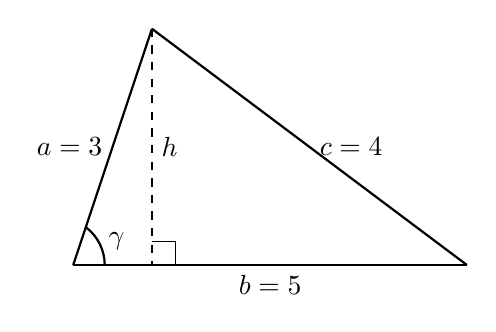
\begin{tikzpicture}
			
			% Draw triangle
			\draw[thick] (0,0) -- (5,0) node[midway, below]{$b=5$};  % Side b
			\draw[thick] (0,0) -- (1,3) node[midway, left]{$a=3$};   % Side a
			\draw[thick] (5,0) -- (1,3) node[midway, right]{$c=4$};  % Side c
			
			% Draw height h
			\draw[dashed] (1,3) -- (1,0) node[midway, right]{$h$};  % Height h
			\draw (1,0.3)-- (1.3,0.3); 
			\draw (1.3,0.3)-- (1.3,0); 
			
			% Mark angle gamma
			\draw[thick] (0.4,0) arc[start angle=0, end angle=52, radius=0.6cm];
			\node at (0.55, 0.3) {$\gamma$};
			
		\end{tikzpicture}
		
		
		\textbf{Constraint}: The given parameters \textbf{must} be initialized as integer values:
		
		\begin{lstlisting}
			int a = 3, b = 5, c = 4, area = 6;
		\end{lstlisting}
		
		
		\item You are given an array \codebox{prices} where each element \codebox{prices[i]} represents the historical price of a stock on the i-th day. Your goal is to find the maximum profit you could have by selecting one day to buy the stock and a later day to sell it. Write a function that returns the maximum profit you could earn from this transaction. If no profit can be made, return \codebox{0}.
		
		\textit{Example 1}:
		\begin{itemize}
			\item \textit{Inputs}: \codebox{prices = [8, 1, 6, 4, 7, 4]}
			
			\item \textit{Output}: \codebox{6}
			
			\item \textit{Explanation}: Buy the stock on day 2 ($price = 1$) and sell on day 5 ($price = 7$), resulting in a profit of $7-1=6$. Note that you must buy the stock before you sell it, so buying on day 2 and selling on day 1 is not valid.
		\end{itemize}
		
		
		
		\textit{Example 2}:
		
		\begin{itemize}
			\item \textit{Inputs}: \codebox{8, 7, 5, 2, 1}
			
			\item \textit{Output}: \codebox{0}
			
			\item \textit{Explanation}: In this case, no transaction results in a profit, so the maximum profit is 0.
		\end{itemize}
		
		
		\textit{IMPORTANT NOTES}:
		\begin{itemize}
			\item Write the code for \codebox{maxProfit()} and \codebox{int main()} testing the function with an example.
			\item Use a \codebox{printf()} within \codebox{int main()} to print the returned value from the function.
			\item Your code must work on any OS.
		\end{itemize}
		
		\item You are given an array \codebox{cost} where each element \codebox{cost[i]} represents the cost to step on the i-th step of a staircase. After paying the cost, you can either move up one or two steps. You can choose to begin at either step 0 or step 1. Write a function that returns the minimum cost required to reach the top of the staircase.
		
		
		\textit{Example 1}:
		
		\begin{itemize}
			\item \textit{Inputs}: \codebox{cost = [8, 12, 20]}
			
			\item \textit{Output}: \codebox{12}
			
			\item \textit{Explanation}: Start at index 1, pay 12, and take two steps to the top. The total cost is 12.
		\end{itemize}
		
		
		
		\textit{IMPORTANT NOTES}:
		\begin{itemize}
			\item Write the code for \codebox{minCostClimbingStairs()} and \codebox{int main()} testing the function with an example.
			\item Use a \codebox{printf()} within \codebox{int main()} to print the returned value from the function.
			\item Your code must work on any OS.
		\end{itemize}
		
		
		
		
		
		\item Given an array of integers \codebox{numbers} that is already sorted in non-decreasing order, \textbf{return} \codebox{true} if there are two numbers such that they add up to a specific \codebox{target} number. If there is no combination of two values such that their sum equals the \codebox{target}, then \textbf{return} \codebox{false}. \textbf{You may not use the same element twice}.
		
		\textit{Example 1}:
		\begin{itemize}
			\item \textit{Inputs} to \codebox{twoSum()} function are: \codebox{numbers = [2,7,11,15]}, \codebox{target = 18}
			
			\item \textit{Output}: \codebox{true}
			
			\item \textit{Explanation}: The sum of 7 and 11 is 18. 
		\end{itemize}
		
		
		
		%	\textbf{Example 2}:
		%	
		%	\textit{Inputs} to \codebox{twoSum()} function are: \codebox{numbers = [2,3,4]}, \codebox{target = 6}
		%	
		%	\textit{Output}: \codebox{true}
		%	
		%	\textit{Explanation}: The sum of 2 and 4 is 6. 
		
		\textit{Example 2}:
		\begin{itemize}
			\item \textit{Inputs} to \codebox{twoSum()} function are: \codebox{numbers = [-3,-1]}, \codebox{target = -2}
			
			\item \textit{Output}: \codebox{false}
			
			\item \textit{Explanation}: There is not a set of two \textbf{different} numbers that their sum would be equal to -2. 
		\end{itemize}		
		
		
		
		
		\textit{Constraints:}
		\begin{itemize}
			\item $2 \leq$ the length of array \codebox{numbers} $\leq 3 \times 10^4$
			%		\item $-1000 \leq \codebox{numbers[i]} \leq 1000$
			\item \codebox{numbers} is sorted in non-decreasing order.
			%		\item $-1000 \leq \codebox{target} \leq 1000$
			\item The data type \codebox{int} (32-bits integer) is acceptable for both \codebox{numbers} and \codebox{target}.
		\end{itemize}
		
		\textit{IMPORTANT NOTES}:
		\begin{itemize}
			\item Write the code for \codebox{twoSum()} and \codebox{int main()} testing the function with an example.
			\item Use a \codebox{printf()} within \codebox{int main()} to print the returned value from the function.
			\item Your code must work on any OS.
		\end{itemize}
		
		
		
		\item 	The Tribonacci sequence $T_n$ is defined as follows:
		
		\[
		T_0 = 0, \quad T_1 = 1, \quad T_2 = 1, \quad \text{and} \quad T_{n+3} = T_n + T_{n+1} + T_{n+2} \quad \text{for} \quad n \geq 0.
		\]
		
		Given n, \textbf{return} the value of $T_n$.
		
		\textit{Example 1}:
		
		\begin{itemize}
			\item \textit{Input}: $n = 5$
			\item \textit{Output}: $output = 7$
			\item \textit{Explanation}: 
			
			\[
			T_3 = 0 + 1 + 1 = 2
			\]
			\[
			T_4 = 1 + 1 + 2 = 4
			\]
			\[
			T_5 = 1 + 2 + 4 = 7
			\]
		\end{itemize}
		
		
		
		\textit{Example 2}:
		
		If $n = 40$, then the output is 12960201916.
		
		\textit{Constraints:}
		\begin{itemize}
			\item The answer is guaranteed to fit within a \textbf{64-bit integer}, i.e., \textbf{answer} $\leq 2^{63} - 1$.
		\end{itemize}
		
		\textit{IMPORTANT NOTES}:
		\begin{itemize}
			\item Write the code for \codebox{tribonacci()} and \codebox{int main()} testing the function with an example.
			\item Use a \codebox{printf()} within \codebox{int main()} to print the returned value from the function.
			\item Your code must work on any OS.
		\end{itemize}
		
		
		\item An anagram is a word or phrase formed by rearranging the letters of another word or phrase, using all the original letters exactly once. You are given two strings, \codebox{s} and \codebox{t}. Write a function that checks whether \codebox{t} is an anagram of \codebox{s}. The function should return \codebox{true} if they are anagrams, and \codebox{false} if they are not. You \textbf{must} write the code with time complexity of $O(n)$.
		
		\textit{Example 1}:
		\begin{itemize}
			\item \textit{Input}: \codebox{s = "listen"}, \codebox{t = "silent"} 
			\item \textit{Output}: \codebox{true}
		\end{itemize}
		
		
		
		\textit{Example 2}:
		\begin{itemize}
			\item \textit{Input}: \codebox{s = "bob"}, \codebox{t = "rob"} 
			\item \textit{Output}: \codebox{false}
		\end{itemize}
		
		
		\textit{IMPORTANT NOTES:}
		\begin{itemize}
			\item Just a hint about $O(n)$ time complexity for this problem, you can use the same method we used during the lecture.
			\item Write the function in the following format:
			\begin{lstlisting}
				bool isAnagram(char* s, char* t) {
					
				}
			\end{lstlisting}
			\item Both strings consist only of lowercase English letters.
			\item No need to write \codebox{int main()}.
			\item Your code must work on any OS.
		\end{itemize}
		
		
		\item 	You are given a \textbf{sorted} array of integers \codebox{nums} in ascending order and an integer target. Write a function to search for \codebox{target} in the array. If the \codebox{target} exists, return its index; otherwise, return \codebox{-1}. You \textbf{must} implement a binary search algorithm ($O(log n)$ time complexity).
		
		
		\textit{Example 1}:
		\begin{itemize}
			\item \textit{Input}: \codebox{nums = [-2,0,3,7,12]}, \codebox{target = 7} 
			\item \textit{Output}: \codebox{3}
			\item \textit{Explanation}: The number \codebox{7} is present in the array at index 3.
		\end{itemize}
		
		
		
		\textit{Example 2}:
		\begin{itemize}
			\item \textit{Input}: \codebox{nums = [-2,0,3,7,12]}, \codebox{target = 2} 
			\item \textit{Output}: \codebox{-1}
			\item \textit{Explanation}: The number \codebox{2} is not present in the array, so the function returns \codebox{-1}.
		\end{itemize}
		
		
		\textit{IMPORTANT NOTES:}
		\begin{itemize}
			\item Write the function in the following format:
			\begin{lstlisting}
				int search(int* nums, int numsSize, int target) {
					
				}
			\end{lstlisting}
			\item All integers in \codebox{nums} are unique.
			\item The array \codebox{nums} is sorted in ascending order.
			\item No need to write \codebox{int main()}.
			\item Your code must work on any OS.
		\end{itemize}
		
		
		\item 	You are given a \textbf{sorted} array of integers \codebox{nums} in ascending order and an integer target. Write a function to search for \codebox{target} in the array. If the \codebox{target} exists, return its index; otherwise, return \codebox{-1}. You \textbf{must} implement a binary search algorithm ($O(log n)$ time complexity).
		
		
		
		
		
		
		\textit{Example 1}:
		\begin{itemize}
			\item \textit{Input}: \codebox{nums = [-2,0,3,7,12]}, \codebox{target = 7} 
			\item \textit{Output}: \codebox{3}
			\item \textit{Explanation}: The number \codebox{7} is present in the array at index 3.
		\end{itemize}
		
		
		
		\textit{Example 2}:
		\begin{itemize}
			\item \textit{Input}: \codebox{nums = [-2,0,3,7,12]}, \codebox{target = 2} 
			\item \textit{Output}: \codebox{-1}
			\item \textit{Explanation}: The number \codebox{2} is not present in the array, so the function returns \codebox{-1}.
		\end{itemize}
		
		
		\textit{IMPORTANT NOTES:}
		\begin{itemize}
			\item Write the function in the following format:
			\begin{lstlisting}
				int search(int* nums, int numsSize, int target) {
					
				}
			\end{lstlisting}
			\item All integers in \codebox{nums} are unique.
			\item The array \codebox{nums} is sorted in ascending order.
			\item No need to write \codebox{int main()}.
			\item Your code must work on any OS.
		\end{itemize}
		
		
		
		
		
		
	\end{enumerate}
	
	
	
	
	
	
	
	
	
	\chapter{Intermediate Topics in C}
	
	
	\section*{Introduction}
	
	This chapter builds upon the foundational knowledge of C and introduces essential intermediate concepts that are critical for developing more sophisticated programs. We start with \textbf{Debugging}, teaching you how to identify and resolve errors effectively, a vital skill for any programmer. Then, we cover the use of \textbf{Makefiles}, which simplify the build process for larger projects by automating compilation. Next, we introduce \textbf{Code Organization} by splitting programs into multiple files, improving maintainability and scalability. A comprehensive section on \textbf{Pointers} follows, delving into their use with constants, arrays, function arguments, and return values—key to understanding memory management and data manipulation. Finally, we explore \textbf{Dynamic Memory Allocation}, focusing on functions like \codebox{malloc}, \codebox{calloc}, and \codebox{realloc}, along with handling potential issues like Stack Overflow. This chapter equips you with the tools needed for efficient, modular, and memory-conscious C programming.
	
	
	\section{Debugging in C}\label{sec:debugging}
	
	Debugging in C using the GNU Debugger (GDB) is a powerful technique for identifying and resolving issues in your C programs. GDB allows you to examine and manipulate the execution of your program, helping you understand and fix bugs, analyze program behavior, and gain insights into code execution.
	
	\begin{tcolorbox}[myboxstyle]
		
		{\Large \textbf{\textcolor{cherry}{Do you have GDB on your OS?!}}} GDB is developed by the GNU Project, GDB is the standard debugger for many Unix-like operating systems, including Linux. It is widely used and supported across various platforms. To check if you have GDB installed on your OS you can use \codebox{gdb --version}. For any reason if it was not installed:
		
		\begin{itemize}
			\item On Linux: GDB comes with the compiler but you didn't have it, use \codebox{sudo apt install gdb}.
			
			\item macOS or iOS: Follow these steps:
			
			\begin{enumerate}
				\item Open Terminal and Install Homebrew, a popular package manager for macOS, by executing the following command in Terminal: \codebox{/bin/bash -c "\$(curl -fsSL} \codebox{https://raw.githubusercontent.com/Homebrew/install/HEAD/install.sh)"}				
				
				\item Once Homebrew is installed, use it to install GDB by running the following command: \codebox{brew install gdb}
				
				\item After the installation is complete, you may need to create a certificate to allow GDB to control other processes on your system. Run the following command:
				
				\codebox{codesign --entitlements gdb-entitlement.xml -fs gdb-cert /usr/local}
				\codebox{/bin/gdb}
				
				This step is necessary to grant GDB the necessary permissions for debugging.
				
				\item Finally, you can verify the installation by running: \codebox{gdb --version}
				
			\end{enumerate}
		
		Please note that starting with macOS Catalina (10.15) and later versions, the system's security measures restrict the use of GDB for debugging certain processes, such as system processes or processes that you do not have appropriate permissions for. Additionally, you may need to adjust your system's security settings to allow GDB to function properly. Refer to the \href{https://sourceware.org/gdb/documentation/}{GDB documentation} or online resources for more information on using GDB on macOS and any additional steps that may be required.
			
		\end{itemize}
		
	\end{tcolorbox}
		
	
	To enable debugging with GDB, you need to compile your C code with the \codebox{-g} flag. This flag includes debugging information in the compiled executable, such as symbol tables, source file names, and line number information. This information is crucial for GDB to provide meaningful debugging capabilities.
	
	Instead of \codebox{-g} flag we may use \codebox{-ggdb3} which the debugging information provided in executable object file is in the format of GDB debugger, while \codebox{-g} is more generic and can be used with different debuggers. So, if you are using LLDB, you must use \codebox{-g}.
	
	\begin{tcolorbox}[myboxstyle]
		
		{\Large \textbf{\textcolor{cherry}{Still have problem with GDB?!}}} There is another debugger called \codebox{lldb} that you can use both on Linux or macOS. LLDB (LLVM Debugger) is developed as part of the LLVM project, LLDB is a relatively newer debugger and was designed to be a replacement for GDB. Initially focused on macOS and iOS, it has since expanded to support other platforms like Linux and Windows. This time I am sure \codebox{lldb} should be on macOS because it comes with the compiler!! But if it doesn't please let me know. Because I don't have macOS I might be wrong!
		
		On Linux although you may need to install it. To check if you have it use: \codebox{lldb --version}. If you don't install it with \codebox{sudo apt install lldb}.
		
	\end{tcolorbox}
	
	
	Here are the differences between different levels of \codebox{-ggdb} flags:
	
	\begin{itemize}
		\item \codebox{-ggdb0}: This level disables debugging information generation. It is equivalent to not using the -g flag at all.
		
		\item \codebox{-ggdb1}: This level generates minimal debugging information. It includes basic symbol table entries and line number information. It is the minimum level recommended for effective debugging.
		
		\item \codebox{-ggdb2}: This level generates additional debugging information, including macro definitions and more detailed symbol table entries. It provides more comprehensive debugging support than -ggdb1.
		
		\item \codebox{-ggdb3}: This level generates the maximum amount of debugging information. It includes extra information for local variables and optimizations. It provides the most detailed debugging support but may increase compilation time and executable size.
	\end{itemize} 
	
	When using GDB or LLDB, you can set breakpoints, step through the code, inspect variable values, examine the call stack, and perform various debugging operations to understand the program's behavior. GDB or LLDB allows you to interactively debug your program, making it a valuable tool for troubleshooting complex issues.
	
	To start debugging with GDB, use the command \codebox{gdb <executable\_name>} or in your terminal, where \codebox{<executable\_name>} is the name of the compiled executable. If you are using LLDB you can do the same by \codebox{lldb <executable\_name>}. Once in the GDB environment (or LLDB), you can use various commands to navigate, inspect, and manipulate your program's execution.
	
	Remember to remove the \codebox{-ggdb} or \codebox{-g} flag when compiling your code for production or release builds, as it adds extra information and increases the executable's size. The \codebox{-ggdb} or \codebox{-g} flags are intended for development and debugging purposes only. Here's an example of C code that uses a while loop, along with some common GDB commands:
	
	\begin{lstlisting}
		#include <stdio.h>
		
		int main() {
			int i = 0;
			
			while (i < 10) {
				printf("Iteration %d\n", i);
				i++;
			}
			printf("The end of loop\n");
		}
	\end{lstlisting}
	
	
	To compile this code with the -ggdb3 flag for maximum debugging information, you can use the following command:
	
	\codebox{gcc -ggdb3 pedram.c -o pedram}
	
	\begin{tcolorbox}[myboxstyle]
		
		{\Large \textbf{\textcolor{cherry}{Tips!}}} There is no different between 
		
		\codebox{gcc -ggdb3 pedram.c -o pedram}
		
		and 
		
		\codebox{gcc -ggdb3 -o pedram pedram.c}
		
	\end{tcolorbox}
	
	
	Once compiled, you can start debugging the program using \codebox{gdb ./pedram}(or \codebox{lldb ./pedram} if you are using LLDB). Here's an example of using some common GDB or LLDB commands:
	
	
	
	\begin{itemize}
		\item \textbf{Setting a Breakpoint}: You can set a breakpoint at a specific line of code using the break command. For example, to set a breakpoint at line 8 (inside the while loop), use \codebox{break 8}. If you are using LLDB you can do the same by \codebox{breakpoint set --line 8}.
                                                                
		\item \textbf{Starting Execution}: In both GDB and LLDB, once a breakpoint is set, you can start the execution of the program using the \codebox{run} command. Although you may set more breakpoints during debugging.
		
		\item \textbf{Stepping through the Code}: In both GDB and LLDB, to step through the code line by line, you can use the \codebox{next} or \codebox{n} command. It will execute the current line and stop at the next line.
		
		\item \textbf{Continuing Execution}: In both GDB and LLDB, if you want to continue execution after hitting a breakpoint or stopping at a specific line, you can use the \codebox{continue} or \codebox{c} command.
		
		\item \textbf{Printing Variable Values}: In both GDB and LLDB, to print the value of a variable during debugging, you can use the \codebox{print} or \codebox{p} command. For example, \codebox{print i} will print the value of the variable \codebox{i}.
		
		\item \textbf{Quitting GDB or LLDB}: To exit the GDB or LLDB debugger, you can use the \codebox{quit} command.
		
	\end{itemize}
	
	Here's an example of how you might interact with GDB using the code provided:
	
	\begin{mdframed}[style=myboxstyleTerminal1]
		\begin{verbatim}
			For help, type "help".
			--Type <RET> for more, q to quit, c to continue without paging--c
			Type "apropos word" to search for commands related to "word"...
			Reading symbols from ./pedram...
			(gdb) break 7
			Breakpoint 1 at 0x117e: file pedram.c, line 7.
			(gdb) run
			Starting program: /home/pedram/Cfolder/pedram 
			[Thread debugging using libthread_db enabled]
			Using host libthread_db library "/lib/x86_64-linux-gnu/libthread_db.so.1".
			
			Breakpoint 1, main () at pedram.c:7
			7               printf("Iteration %d\n", i);
			(gdb) continue
			Continuing.
			Iteration 0
			
			Breakpoint 1, main () at pedram.c:7
			7               printf("Iteration %d\n", i);
			(gdb) next
			Iteration 1
			8               i++;
			(gdb) print i
			$1 = 1
			(gdb) c
			Continuing.
			
			Breakpoint 1, main () at pedram.c:7
			7               printf("Iteration %d\n", i);
			(gdb) c
			Continuing.
			Iteration 2
			
			Breakpoint 1, main () at pedram.c:7
			7               printf("Iteration %d\n", i);
			(gdb) p i
			$2 = 3
			(gdb) exit
			A debugging session is active.
			
			Inferior 1 [process 61784] will be killed.
			
			Quit anyway? (y or n) y
		\end{verbatim}
	\end{mdframed}
	
	Using these additional flags can provide more comprehensive warning messages and enforce stricter adherence to the C language standard. They can help catch potential issues, improve code quality, and ensure compliance with best practices. Here is a list of some useful flags:
	
	\begin{itemize}
		
		\item \codebox{-Wall} enables additional warning messages during compilation. It enables common warnings that help catch potential issues and improve code quality.
		
		\item \codebox{-Wextra} enables even more warning messages beyond those enabled by -Wall. It includes additional warnings that are not included in -Wall.
		
		\item \codebox{-Wconversion} generates warnings for implicit type conversions that may cause loss of data or unexpected behavior.
		
		\item \codebox{-Wsign-conversion} generates warnings for implicit sign conversions, where signedness is changed during assignments or comparisons.
		
		\item \codebox{-Wshadow} generates warnings for variable shadowing, which occurs when a variable in an inner scope has the same name as a variable in an outer scope.
		
		\item \codebox{-Wpedantic} generates warnings for strict ISO C adherence. It enables additional warnings that follow the strictest interpretation of the C language standard.
		
		\item \codebox{-std=c17} specifies the C language standard to be used during compilation. In this case, it specifies the C17 standard, which is the ISO/IEC 9899:2017 standard for the C programming language.
		
	\end{itemize}
	
	Quite easy to use! To compile the same program you can use:
	
	\codebox{gcc -ggdb3 -Wall -Wextra -Wconversion -Wsign-conversion -Wshadow -Wpedantic}
		
	\codebox{-std=c17 pedram.c -o pedram}
	
	Debugger uses these flags to include almost full information about the code in the object file during compiling. Sometimes you are testing your program and you may need to compile your code many times. Every time adding these flags might be time consuming. That's where we might need \hyperref[subsec:makefile]{\textcolor{orange!80!black}{Makefile}}.
	
	
	
	
	
	
	
	
	
	\section{Makefile}\label{sec:makefile}
	
	A Makefile is a text file that contains a set of rules for compiling and building programs. It is used to automate the compilation process by specifying dependencies, compilation flags, and target outputs. Makefiles are commonly used in C projects to simplify building and managing complex codebases.
	
	\textbf{Why we need Makefile}? Makefiles provide a convenient way to manage the compilation process and handle dependencies in C projects. They allow developers to specify the relationships between different source files and ensure that only the necessary files are recompiled when changes are made. Makefiles also make it easier to manage build configurations, compilation flags, and linking options. Overall, Makefiles streamline the build process and help maintain code consistency and reproducibility.
	
	Makefiles consist of rules, targets, dependencies, and commands. Here's an overview of some key components:
	
	\begin{itemize}
		\item \textbf{Rules}: Rules define the relationship between targets and dependencies. They specify how to build targets from dependencies.
		
		\item \textbf{Targets}: Targets represent the desired outputs, such as executable files or object files. They can be source files, intermediate files, or final build artifacts.
		
		\item \textbf{Dependencies}: Dependencies are files or other targets that are required to build a specific target. If a dependency is modified, the corresponding target needs to be rebuilt.
		
		\item \textbf{Commands}: Commands are the actual shell commands executed to build a target. They specify how to compile source files, link object files, and generate the final output.
	\end{itemize}
	
	This is the general format of Makefile(s):
	
	\begin{lstlisting}
		target: prerquisites
		(TAB) command line(s)
	\end{lstlisting}
	
	Where:
	
	\begin{itemize}
		\item Left side of \codebox{:} is the \textbf{target} to be built,
		\item Right side of \codebox{:} files (\textbf{Dependencies}) which \textbf{target} depends on,
		\item Line(s) start with a TAB if the next line is a command,
		\item Each line ends with \codebox{ENTER},
		\item Line(s) started with \codebox{\#} are Comments.
	\end{itemize}
	
	Let's take a look at the following example save in the source code named \codebox{factorial.c}.
	
	\begin{lstlisting}
		#include <stdio.h>
		
		int factorial(int n) {
			if (n == 0 || n == 1) {
				return 1;
			}
			return n * factorial(n - 1);
		}
		
		int main() {
			int num = 5;
			int result = factorial(num);
			printf("Factorial of %d is %d\n", num, result);
			return 0;
		}
	\end{lstlisting}

	Using the following command line in the terminal, I can compile the code and create the executable object file \codebox{pedram}:
	
	\begin{lstlisting}
		gcc -o pedram factorial.c -Wall -Wextra -std=c99
	\end{lstlisting}

	Now we want to do the same with a \codebox{Makefile}. Open a terminal and use \codebox{nano Makefile}. Copy and paste the following code and save the file.
	
	\begin{lstlisting}
		pedram: factorial.c
			gcc -o pedram factorial.c -Wall -Wextra -std=c99
	\end{lstlisting}
	
	Make sure there is a TAB space behind \codebox{gcc}, one four \codebox{Space bar} on keyboard. You can open the \codebox{Makefile} file on VScode, or on a Text Editor. \codebox{Makefile}s are better to be opened on Text Editor since they show the difference between four \codebox{Space bar} and TAB space. In this Makefile:
	
	\begin{itemize}
		\item \codebox{pedram} is specified as the target,
			
		\item \codebox{factorial.c} is listed as a prerequisite for \codebox{pedram}, meaning \codebox{pedram} depends on, \codebox{factorial.c}. This ensures that if \codebox{factorial.c} changes, \codebox{pedram} will be rebuilt,
		
		\item The command \codebox{gcc -o pedram factorial.c} is used to compile \codebox{factorial.c} \textbf{directly} into the \codebox{pedram} executable without generating an intermediate object file.
	\end{itemize}

	Make sure that you have created \codebox{Makefile} in the same directory that the source code \codebox{factorial.c} is saved. In a terminal with the directory that both files are located in, execute \codebox{make}. \codebox{make} searches for a file with name \textbf{makefile} in the current directory I If there is no such a file, make searches for a file with name \textbf{Makefile}. This is what \textbf{I} see in your \textbf{terminal}:
	
	\begin{lstlisting}
		pedram@pedram-GL553VE:~/Cfolder/practice/lec$ make
		gcc -o pedram factorial.c -Wall -Wextra -std=c99
	\end{lstlisting}

	Check the directory and you will find the object file \codebox{pedram}, and you can execute the program the same as always with \codebox{./pedram}. If I remove the TAB before the command line in the \codebox{Makefile}, like:
	
	\begin{lstlisting}
		pedram: factorial.c
		gcc -o pedram factorial.c -Wall -Wextra -std=c99
	\end{lstlisting}

	Then, in the terminal I see the following error:
	
	\begin{lstlisting}
		Makefile:15: *** missing separator.  Stop.
	\end{lstlisting}

	If I keep the TAB, but remove the line \codebox{pedram: factorial.c}, then I get the following message:
	
	\begin{lstlisting}
		Makefile:15: *** recipe commences before first target.  Stop.
	\end{lstlisting}

	Both mean the object file \codebox{pedram} is not made yet. Every time I use \codebox{make}, file(s) will be created in the current directory. In this case it is only the final executable file named \codebox{pedram}. Some times instead of removing them manually, I can use the \codebox{clean} command in the directory to remove the files. For example with the 2nd version of \codebox{Makefile}:


	\begin{lstlisting}
		pedram: factorial.c
			gcc -o pedram factorial.c -Wall -Wextra -std=c99
		
		clean:
			rm -f pedram
	\end{lstlisting}

	I can type in the terminal \codebox{make clean} and it will remove (\codebox{rm}) the file ()\codebox{-f}) named \codebox{pedram} from the current directory.
	
	
	\begin{tcolorbox}[myboxstyle]
		
		{\Large \textbf{\textcolor{cherry}{WARNING!}}} The line \codebox{rm -f} will remove any file name given from the directory. For example, if I use \codebox{rm -f pedram <other files>}, the other files will be removed!!
		
	\end{tcolorbox}
	
	
	
	In the context of your \codebox{Makefile} examples, \textbf{macros} (also known as variables in Make) are used to define reusable values that can be referenced throughout the \codebox{Makefile}. Several useful macros are:
		
	\begin{itemize}
		\item \codebox{CC}: Represents the compiler (\codebox{gcc}).
		\item \codebox{CFLAGS}: Represents the compiler flags (\codebox{-Wall -Wextra -std=c99}).
		\item \codebox{EXECUTABLE}: Represents the name of the executable (\codebox{pedram}).
		\item \codebox{SRC}: Represents the source file (\codebox{factorial.c}).
	\end{itemize}

	\textbf{Why} macros are useful? Making the long story short, macros in \codebox{Makefiles} improve readability, maintainability, consistency, flexibility, and help avoid repetition, making it easier to manage and modify complex build processes. With Macros I can write the same \codebox{Makefile} like:
	

	\begin{lstlisting}
		CC = gcc
		CFLAGS = -Wall -Wextra -std=c99
		EXECUTABLE = pedram
		SRC = factorial.c
		
		$(EXECUTABLE): $(SRC)
			$(CC) $(CFLAGS) -o $@ $^
		
		clean:
			rm -f $(EXECUTABLE)
	\end{lstlisting}
	
	
	The way you program is \textbf{unique} like your \textbf{handwriting}, or unique to the way you think. I can create the object file \codebox{pedram}, with another type of handwriting:
	
	
	\begin{lstlisting}
		pedram: factorial.o
			gcc -o pedram factorial.o
		
		factorial.o: factorial.c
			gcc -c factorial.c -Wall -Wextra -std=c99
		
		clean:
			rm -f pedram factorial.o
	\end{lstlisting}
	
	\codebox{factorial.o} is an object file generated by compiling the \codebox{factorial.c} source file. In C and C++ programming, when you compile a source file (\codebox{.c} file), the compiler produces an object file (\codebox{.o} file) as an intermediate step before creating the final executable. Here's what each line does:
	
	\begin{enumerate}
		\item \codebox{pedram: factorial.o}: This line indicates that the target \codebox{pedram} depends on \codebox{factorial.o}. In other words, before creating the \codebox{pedram} executable, Make needs to ensure that \codebox{factorial.o} is up-to-date.
		\item \codebox{gcc -o pedram factorial.o}: This is the rule to build the \codebox{pedram} executable. It specifies that \codebox{pedram} depends on \codebox{factorial.o}, and to create \codebox{pedram}, the command:
		
		\codebox{gcc -o pedram factorial.o}
		
		is executed. This command links the \codebox{factorial.o} object file to produce the final executable named \codebox{pedram}.
		
		\item \codebox{factorial.o: factorial.c}: This line indicates that the \codebox{factorial.o} object file depends on \codebox{factorial.c}. If \codebox{factorial.c} is newer than \codebox{factorial.o}, Make will rebuild \codebox{factorial.o}.
		
		\item \codebox{gcc -c factorial.c}: This is the rule to compile \codebox{factorial.c} into \codebox{factorial.o}. The \codebox{-c} flag tells the compiler to generate the object file without linking, so it produces \codebox{factorial.o} instead of an executable.
	\end{enumerate}

	\textbf{Why} did I add \codebox{-Wall -Wextra -std=c99} to \codebox{factorial.o: factorial.c} not the other one? After \codebox{make} in the terminal I get:
	
	\begin{lstlisting}
		gcc -c factorial.c -Wall -Wextra -std=c99
		gcc -o pedram factorial.o 
	\end{lstlisting}
	
	If I \codebox{make clean}, then in the terminal I get:
	
	\begin{lstlisting}
		rm -f pedram factorial.o
	\end{lstlisting}

	\begin{tcolorbox}[myboxstyle]
		
		{\Large \textbf{\textcolor{cherry}{Kind of IMPORTANT!}}} After I pass the command \codebox{make} in the terminal, I create \codebox{pedram} executable object file, and \codebox{factorial.o} object file. I can execute the program by \codebox{./pedram}, but not with \codebox{./factorial.o}. Now let's \textbf{remove} the \codebox{-c} while doing \codebox{factorial.o: factorial.c}. The this is what I see in the terminal:
		\begin{mdframed}[style=myboxstyleTerminal1]
			\begin{verbatim}
				pedram@pedram-GL553VE:~/Cfolder/practice$ make
				gcc factorial.c -Wall -Wextra -std=c99
				gcc -o pedram factorial.o
				/usr/bin/ld: cannot find factorial.o: No such file or directory
				collect2: error: ld returned 1 exit status
				make: *** [Makefile:2: pedram] Error 1
			\end{verbatim}
		\end{mdframed}
		This means that the line 2 (\codebox{gcc -o pedram factorial.o}), was not executed, meaning the object file \codebox{pedram} was not created. \codebox{pedram} is depended on \codebox{factorial.o} which tells me potentially the problem is \codebox{factorial.o}. By \textbf{removing} \codebox{-c} the source code \codebox{factorial.c} is directly compile into the executable file \codebox{factorial.o}. In terminal I can run the program this time with \codebox{./factorial.o}. 
		
		My point is intentionally introduce errors to Makefiles we have here by removing some syntax. Then try to logically find the issue. Les's say in the next version of \codebox{Makefile}, remove \codebox{-c} or \codebox{\$<}.
	\end{tcolorbox}
	
	With Macros I can write the same \codebox{Makefile} with the following format:

	\begin{lstlisting}
		CC = gcc
		CFLAGS = -Wall -Wextra -std=c99
		EXECUTABLE = pedram
		SRC = factorial.c
		OBJ = factorial.o
		
		$(EXECUTABLE): $(OBJ)
			$(CC) -o $@ $^
		
		$(OBJ): $(SRC)
			$(CC) -c $(CFLAGS) $< -o $@
		
		clean:
			rm -f $(EXECUTABLE) $(OBJ)
	\end{lstlisting}

	In this Makefile:
	
	\begin{itemize}
		\item \codebox{CC} is the compiler macro.
		\item \codebox{CFLAGS} contains compiler flags.
		\item \codebox{EXECUTABLE} is the macro for the executable name.
		\item \codebox{SRC} is the source file macro.
		\item \codebox{OBJ} is the object file macro.
	\end{itemize}

	In a Makefile, \codebox{\$@} and \codebox{\$\^} are automatic variables used to represent the target and all prerequisites of a rule, respectively. Also \codebox{\$<} is an automatic variable that represents the first prerequisite of the target.
	
	\begin{itemize}
		\item \codebox{\$@} is replaced with the name of the target, which is \codebox{\$(EXECUTABLE)}, i.e., \codebox{pedram}.
		
		\item \codebox{\$\^} is replaced with the list of prerequisites, which is \codebox{\$(OBJ)}, i.e., \codebox{factorial.o}.
		
		\item \codebox{\$<} is replaced with the name of the first prerequisite, which in this case is \codebox{\$(SRC)}, or \codebox{factorial.c}, or the right side.
	\end{itemize}
	
	Using the command \codebox{make -p} line, you will find all the symbols we use in the makefile. Not really user-friendly to follow though! 
	
	Using macros makes it easier to modify the \codebox{Makefile} if necessary, as you only need to change the values of the macros. For example, if you change the source file or add more source files, you only need to update the \codebox{SRC} macro. Similarly, changing the compiler or compiler flags can be done by modifying the corresponding macros.
	
	Keep the latest version of \codebox{Makefile}, and pass \codebox{make} command in the terminal. We will see:
	
	\begin{lstlisting}
		gcc -c -Wall -Wextra -std=c99 factorial.c -o factorial.o
		gcc -o pedram factorial.
	\end{lstlisting}

	If I do it one more time I get:
	
	\begin{mdframed}[style=myboxstyleTerminal1]
		\begin{verbatim}
			make: 'pedram' is up to date.
		\end{verbatim}
	\end{mdframed}
	
	Pass the command \codebox{make clean}. \textbf{Then}, execute \codebox{make -n}. \codebox{make -n} is used to perform a "dry run" of a Makefile. It doesn't actually execute the commands specified in the \codebox{Makefile}; instead, it prints the commands it would execute without actually executing them. This is useful for understanding what actions make would take without affecting the filesystem.
	
	Use \codebox{cat -v -t -e Makefile} in the terminal. This is what I see in the terminal:
	
	\begin{lstlisting}
		CC = gcc$
		CFLAGS = -Wall -Wextra -std=c99$
		EXECUTABLE = pedram$
		SRC = factorial.c$
		OBJ = factorial.o$
		$
		$(EXECUTABLE): $(OBJ)$
		^I$(CC) -o $@ $^$
		$
		$(OBJ): $(SRC)$
		^I$(CC) -c $(CFLAGS) $< -o $@$
		$
		clean:$
		^Irm -f $(EXECUTABLE) $(OBJ)$
		$
		# this is a comment$
	\end{lstlisting}
	
	\begin{tcolorbox}[myboxstyle]
		
		{\Large \textbf{\textcolor{cherry}{Reminder!}}} There is a \codebox{TAB} space before the line starting with \codebox{\$(CC) ...} and \codebox{rm -f ...} (commands). For some reason that baffle even the most seasoned programmers!!! this \codebox{TAB} space format is different in VScode when you are writing a Makefile and probably you would encounter errors like:
		
		\begin{mdframed}[style=myboxstyleTerminal1]
			\begin{verbatim}
				Makefile:7: *** missing separator.  Stop.
			\end{verbatim}
		\end{mdframed}
		
		To avoid this problem forget about VScode when writing Makefiles. Format you Makefile when you run \codebox{nano Makefile} by removing extra spaces and entering \codebox{TAB} spaces before mentioned lines. You can also edit your Makefile in the \textbf{Text Editor} environment by running \codebox{open Makefile}, which opens the file by \textbf{Text Editor} after making it with \codebox{nano}. The difference is clear in the textbf{Text Editor}.
		
	\end{tcolorbox}
	
	We used the command \codebox{cat} first chapter. The flags are:
	
	\begin{itemize}
		\item \codebox{-v}: Display non-printing characters visibly. This option shows non-printing characters in a way that they can be easily identified, such as showing tabs as \codebox{\^I}.
		
		\item \codebox{-t}: Display tab characters (\codebox{\^I}) as \codebox{\^I}. This option specifically handles tab characters and displays them as \codebox{\^I}.
		
		\item \codebox{-e}: Display end-of-line markers (\codebox{\$}) at the end of each line. This option adds a dollar sign \codebox{\$} at the end of each line, indicating the end of the line.
	\end{itemize}
	

	
	
	
	
	
	
	
	\section{Code Organization}
	
	Splitting code into multiple files is a common practice in programming, including in languages like C. This modular approach offers several benefits and allows for better organization, readability, and maintainability of codebases. Splitting code into multiple files offers advantages such as:
	
	\begin{itemize}
		\item \textbf{Modularization}: Breaking code into smaller, more manageable units improves organization and readability.
		\item \textbf{Re-usability}: Code can be reused across different projects by linking or including the appropriate files.
		\item \textbf{Maintainability}: Isolating different functionalities or modules in separate files makes it easier to update or modify specific parts without affecting the entire codebase.
		\item \textbf{Compilation Efficiency}: When changes are made to a single file, only that file and its dependencies need to be recompiled, saving compilation time.
	\end{itemize}
	
	By separating code into multiple files, developers can better structure their projects, collaborate more effectively, and build scalable and maintainable software systems. So far we have programmed only in source code files (\codebox{.c} in C or \codebox{.cpp} in C++). 
	
	\begin{itemize}
		\item Source code files contain the actual implementation of functions, variables, and other program logic.
		\item Each source code file typically corresponds to a specific module or functionality of the program.
		\item They include the necessary header files to gain access to the declarations and definitions needed for the code to compile and run.
	\end{itemize}
	
	You can make your own Header Files (\codebox{.h} in C or \codebox{.hpp} in C++). 
	
	\begin{itemize}
		\item Header files contain function prototypes, type definitions, macro definitions, and other declarations that need to be shared across multiple source code files.
		They typically define interfaces and provide a way to communicate between different parts of a program.
		\item Header files are meant to be included in source code files (.c or .cpp) using the \codebox{\#include} directive.
		\item They help in maintaining a separation between interface and implementation, making the code more modular and reusable.
	\end{itemize}
	
	Here's an example of C code with a main source file (\codebox{main.c}) and a corresponding header file (\codebox{functions.h}). Save the following code in \codebox{main.c}:
	
	\begin{lstlisting}
		#include <stdio.h>
		#include "functions.h"
		
		int main() {
			int num = 5;
			int result = square(num);
			
			printf("Square of %d is %d\n", num, result);
		}
	\end{lstlisting}
	
	By now you can see VScode even without compiling is giving you an error indicating that it cannot find \codebox{functions.h}. Create a file named \codebox{functions.h} and paste the following code into it:
	
	\begin{lstlisting}
		#ifndef FUNCTIONS_H
		#define FUNCTIONS_H
		
		int square(int num) {
			return num * num;
		}
		
		#endif
	\end{lstlisting}
	
	The \codebox{\#ifndef FUNCTIONS\_H} and \codebox{\#define FUNCTIONS\_H} directives are known as include guards or header guards. They are used to prevent multiple inclusions of the same header file within a single compilation unit.
	
	When a header file is included in multiple source files, there is a possibility of multiple definitions and declarations, which can lead to compilation errors due to redefinition of symbols. The include guards help avoid these errors by ensuring that the contents of the header file are processed only once during the compilation process.
	
	Create a file named Makefile (no file extension) and paste the following code into it. To avoid the format errors mentioned in the previous section do it on terminal or Text Editor.
	
	\begin{lstlisting}
		CC = gcc
		CFLAGS = -Wall -Wextra
		
		all: main
		
		main: main.c functions.h
							$(CC) $(CFLAGS) -o main main.c
		
		clean:
							rm -f main
	\end{lstlisting}
	
	Let's go through each line of the provided Makefile syntax: 
	\begin{itemize}
		\item \codebox{CC = gcc}: This line assigns the value  \codebox{gcc} to the variable  \codebox{CC}. Here,  \codebox{CC} represents the compiler to be used for compilation.
		
		\item  \codebox{CFLAGS = -Wall -Wextra}: This line assigns the value  \codebox{-Wall -Wextra} to the variable  \codebox{CFLAGS}. Here,  \codebox{CFLAGS} represents the compiler flags or options that are passed to the compiler during compilation. In this case,  \codebox{-Wall and -Wextra} are flags that enable additional compiler warnings.
		
		\item  \codebox{all: main}: This line defines a target \textbf{named}  \codebox{all}. The  \codebox{all} target is considered the default target, meaning that it will be executed if no specific target is provided when running make. In this case, the all target depends on the  \codebox{main} target.
		
		\item  \codebox{main: main.c functions.h}: This line defines the main target. It states that the  \codebox{main} target \textbf{depends} on  \codebox{main.c} and  \codebox{functions.h} files. If any of these files are modified, the main target will be considered outdated and need to be rebuilt.
		
		\item  \codebox{\$(CC) \$(CFLAGS) -o main main.c}: This line is the recipe for building the  \codebox{main} target. It specifies the commands to be executed to create the  \codebox{main} executable file.
		
		Here's a breakdown of the syntax:
		
		\begin{enumerate}
			\item \codebox{\$(CC)}: This expands the value of the CC variable, which is gcc. So, this represents the compiler command.
			\item \codebox{\$(CFLAGS)}: This expands the value of the CFLAGS variable, which is -Wall -Wextra. So, this represents the compiler flags.
			\item \codebox{-o main}: This specifies the output file name as main.
			\item \codebox{main.c}: This is the source file that is passed to the compiler for compilation.
			\item \codebox{clean: rm -f main}: This line defines the clean target. The clean target is typically used to remove generated files or clean up the project directory. In this case, the clean target specifies the command \codebox{rm -f main} to remove the \codebox{main} executable file.
		\end{enumerate}
		
	\end{itemize}

	In summary, this Makefile specifies a compilation process for building the main executable file. It uses the gcc compiler with the flags -Wall and -Wextra to compile main.c and functions.h. The resulting executable file is named main. Additionally, there is a clean target to remove the generated main file.
	
	Open a terminal, navigate to the directory where the files are saved, and run the following command to compile \codebox{make}. This will compile the code and generate an executable file named \codebox{main}. Run the program by executing \codebox{./main}. You should see the output: "\textbf{Square of 5 is 25}". In this example the implementation of the \codebox{square} function was defined directly inside the \codebox{functions.h}. The other scenario is to declare the function in the header file \codebox{function.h}, but write the actual implementation of \codebox{square} in another source code. This approach has some considerations:
	
	\begin{itemize}
		\item \textbf{Code Organization}: Separating the function implementation into a separate source file (functions.c) allows for better code organization. By having separate files for declarations (header file) and definitions (source file), the codebase becomes more modular and maintainable. It also helps in managing larger projects with multiple functions.
		
		\item \textbf{Compilation Efficiency}: If the function square is defined directly in the header file and included in multiple source files, each source file would have its own copy of the function code. This can lead to code duplication and potentially larger executable sizes. By placing the function definition in a separate source file, the function is compiled only once, and all source files can share the same compiled code.
		
		\item \textbf{Reducing Rebuilds}: When modifications are made to the function implementation in functions.c, only that file needs to be recompiled. If the function definition is directly in the header file, any change to the function will require recompiling all source files that include the header file, even if they don't directly use the function.
		
		\item \textbf{Encapsulation and Information Hiding}: Separating the function implementation in a source file helps hide the implementation details from other source files. The header file provides a clean interface (declarations) for other source files to use the functions without exposing the internal implementation.
	\end{itemize}
	
	If you remember when we are using \codebox{math.h} by including the header file we still get some error saying that the compiler cannot find the actual implementation of the functions used in our code. That's why we used \codebox{-lm} flag to tell compiler where it can find the corresponding source code containing the implementations.
	
	The C library is typically distributed as compiled code, and its source code may not be readily available or accessible to users. The implementation details of library functions, including \codebox{sin()} from \codebox{math.h}, are considered part of the library's internal implementation and are not exposed to the user.
	
	However, the behavior and specifications of these functions are defined in the C standard, and their functionality is well-documented. The C standard provides guidelines on how functions like \codebox{sin()} should behave and what the expected results and behavior are for different input values. In this way, the developer, will not share the codes with users.
	
	This is the most important reason of why sometimes we need to declare the functions in \codebox{.h} files but leave the definitions in a another source code with \codebox{.c} extension. Keep the \codebox{main.c} the same way it was. Change the file \codebox{functions.h} into following code where it contains only declaration of the function:
	
	\begin{lstlisting}
		#ifndef FUNCTIONS_H
		#define FUNCTIONS_H
		
		int square(int num);
		
		#endif
	\end{lstlisting}
	
	
	Create a file named \codebox{functions.c} and paste the following code into it:
	
	\begin{lstlisting}
		#include "functions.h"
		
		int square(int num) {
			return num * num;
		}
	\end{lstlisting}
	
	
	Create a file named Makefile (no file extension) and paste the following code into it:
	
	\begin{lstlisting}
		CC = gcc
		CFLAGS = -Wall -Wextra
		
		all: main
		
		main: main.o functions.o
		$(CC) $(CFLAGS) -o main main.o functions.o
		
		main.o: main.c functions.h
		$(CC) $(CFLAGS) -c main.c
		
		functions.o: functions.c functions.h
		$(CC) $(CFLAGS) -c functions.c
		
		clean:
		rm -f main *.o
	\end{lstlisting}
	
	Let's go through each line of the provided syntax in the context of a Makefile:
	
	\begin{itemize}
		\item \codebox{main: main.o functions.o}: This line specifies the target main and lists its dependencies as \codebox{main.o} and \codebox{functions.o}. This means that the target main depends on the object files \codebox{main.o} and \codebox{functions.o}. If any of these object files are modified, the main target will be considered outdated and need to be rebuilt.
		
		\item \codebox{main.o: main.c functions.h}: This line specifies the target \codebox{main.o} and lists its dependencies as \codebox{main.c} and \codebox{functions.h}. This means that the target \codebox{main.o} depends on the source file \codebox{main.c} and the header file \codebox{functions.h}. If any of these files are modified, the \codebox{main.o} target will be considered outdated and need to be rebuilt.
		\item \codebox{functions.o: functions.c functions.h}: This line specifies the target \codebox{functions.o} and lists its dependencies as \codebox{functions.c} and \codebox{functions.h}. This means that the target functions.o depends on the source file \codebox{functions.c} and the header file \codebox{functions.h}. If any of these files are modified, the \codebox{functions.o} target will be considered outdated and need to be rebuilt.
	\end{itemize}

	In summary, this Makefile defines targets for building the main executable, \codebox{main.o}e object file, and \codebox{functions.o} object file. The main target depends on the \codebox{main.o} and \codebox{functions.o} object files, which in turn depend on the corresponding source files and header files. The compiler commands specified in the recipes compile the source files into object files using the provided flags (\codebox{\$(CFLAGS)}) and link the object files together to create the final executable. If any of the source files or header files are modified, the respective targets will be considered outdated and need to be rebuilt. To practice this program, put some breakpoints in the code, using GDB or LLDB, to see the order of the lines being executed. To so this:
	
	\begin{enumerate}
		\item First you need to put \codebox{-g} flag in the Makefile. So the object file made by compiler will include some information about GDB. If you skip this part, you might see messages like:
		
		\begin{mdframed}[style=myboxstyleTerminal1]
			\begin{verbatim}
				No symbol table is loaded.  Use the "file" command.
			\end{verbatim}
		\end{mdframed}
		
		when trying to set break points, indicating that \codebox{gdb} or \codebox{lldb} cannot define your make file must be like:
		
		\codebox{CFLAGS = -g -Wall -Wextra}
		
		\item Execute \codebox{make} in the Terminal to make the object file, in this case it must \codebox{main}.
		
		\item Run the \codebox{main} executable under GDB compiler by \codebox{gdb ./main}.
		
		\item If you have copied the code exactly with the same format mentioned above you should have the same order of numbering for the line. Let's say in the \codebox{main.c}, the line number 7 is: \codebox{int result = square(num);}. Define the following break points:
		
		\begin{itemize}
			
			\item \codebox{break main.c:7} will set a breakpoint at line 7:
			
			\codebox{int result = square(num);} 
			
			\vspace{\baselineskip}
			
			\item \codebox{break main.c:9} will set a breakpoint at line 9:
			
			\codebox{printf("Square of \%d is \%d\textbackslash n", num, result);}.
			
			\vspace{\baselineskip}
			
			\item \codebox{break functions.h:4} will set a breakpoint in \codebox{functions.h} at line 4:
			
			\codebox{int square(int num);}.
			
			\vspace{\baselineskip}
			
			\item \codebox{break functions.c:5} will set a breakpoint in \codebox{functions.c} at line 5:
			
			\codebox{return num * num;}.
			
			\vspace{\baselineskip}
			
		\end{itemize}
	
		\item Start the debugging by executing \codebox{run} in the Terminal.
		
		\item Use \codebox{print}, \codebox{next}, \codebox{continue} and so on, to go through the code. If you don't remember this part go back to \hyperref[sec:debugging]{\textcolor{orange!80!black}{Debugging in C}}.

	\end{enumerate}
	
	
	
	
	
	
	
	
	
	
	
	
	
	
	
	
	\section{Pointer}
	
	I think Pointer are the most confusing concept in C. I need your full attention here!! In C programming, memory is divided into bytes, and each byte consists of 8 bits (one byte). Each byte in memory has a unique address that can be used to access or manipulate the data stored in that memory location. A pointer in C is a variable that holds the address of another variable. Pointers allow us to indirectly access and manipulate the data stored in a particular memory location. The syntax for declaring a pointer variable is to use an asterisk (\codebox{*}) before the variable name, followed by the data type it points to. For example:
	
	\begin{lstlisting}
		int *p;          // p is a pointer to an integer
		double *Pedram;  // Pedram is a pointer to a double
	\end{lstlisting}
	
	When we declare a pointer variable like \codebox{int *p};, the pointer \codebox{p} is capable of storing memory addresses that point to an integer. The unary operator \codebox{*} is used to \textbf{de-reference} a pointer, which means accessing the value at the memory location that the pointer points to. For example, if \codebox{p} points to a memory location that contains an integer, \codebox{*p} gives us the value of that integer. The other way around is if a variable is initialized and you want to access the address. If \codebox{a} is a variable in memory, then \codebox{\&a} represents the address where the value of a is stored. In another word, \codebox{*} is the inverse of \codebox{\&}, like a=*\&b is equal to a = b! Take a look at the following example:
	
	\begin{lstlisting}
		#include <stdio.h>
		
		int main() {
			int a = 42;   // Declare and initialize an integer variable
			
			int *p;       // Declare a pointer to an integer
			p = &a;       // Assign the address of 'a' to the pointer 'p'
			/*or we could use int *p = &a;*/ 
			
			printf("Value of 'a': %d\n", a);
			printf("Address of 'a': %p\n", &a); // %p is placeholder
			printf("Value of 'p' (address of 'a'): %p\n", p);
			
			printf("Value pointed by 'p': %d\n", *p); // De-reference p
			
			*p = 500;
			printf("\nPrint out after *p=500.\n");
			printf("Value of 'a': %d\n", a);
			printf("Value pointed by 'p': %d\n", *p);
			
			a = 98;
			printf("\nPrint out after a = 98.\n");
			printf("Value of 'a': %d\n", a);
			printf("Value pointed by 'p': %d\n", *p);
		}
	\end{lstlisting}
	
	In this example, we declared an integer variable \codebox{a} and a pointer \codebox{p} to an integer. At this moment the pointer is not initialized to point to any address. This figure shows how it looks like:
	
	
	\begin{center}
		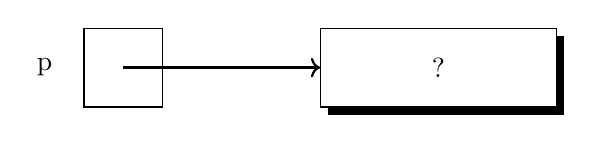
\begin{tikzpicture}
			% Draw the first rectangle
			\draw (4,0) rectangle (5,1);
			\node at (3.5,0.5) {p};
			
			% Draw the arrow
			\draw[->, thick] (4.5,0.5) -- (7,0.5);
			%\node at (6,0.7){p = \&a};
			
			% Draw the second rectangle
			\draw (7,0) rectangle (10,1);
			\node at (8.5,0.5) {?};
			%\node at (8.5,1.3) {0x7fffc2b40dcc};
			%\node at (10.5,0.5) {a};
			\fill[black] (7.1,0) rectangle (10.1,-0.1);
			\fill[black] (10,0) rectangle (10.1,0.9);
		\end{tikzpicture}
	\end{center}
	
	
	The, we assigned the address of \codebox{a} to the pointer \codebox{p} using the address-of operator \codebox{\&}, like the following figure.
	
	\begin{center}
	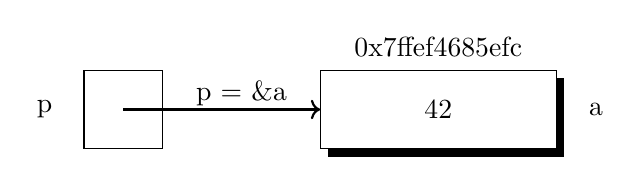
\begin{tikzpicture}
		% Draw the first rectangle
		\draw (4,0) rectangle (5,1);
		\node at (3.5,0.5) {p};
		
		% Draw the arrow
		\draw[->, thick] (4.5,0.5) -- (7,0.5);
		\node at (6,0.7){p = \&a};
		
		% Draw the second rectangle
		\draw (7,0) rectangle (10,1);
		\node at (8.5,0.5) {42};
		\node at (8.5,1.3) {0x7ffef4685efc};
		\node at (10.5,0.5) {a};
		\fill[black] (7.1,0) rectangle (10.1,-0.1);
		\fill[black] (10,0) rectangle (10.1,0.9);
	\end{tikzpicture}
	\end{center}
	
	
	By de-referencing \codebox{p} with \codebox{*p}, we can access the value stored at the address pointed by \codebox{p}, which is the value of \codebox{a}. Here is the output in \textbf{my computer}. I am saying \textbf{my computer}, because the address given to the value \codebox{a} to save it, in your computer will be different. Actually, every time you run the code, you can see a new address is given to save this value. Here is results in my computer:
	
	
	\begin{mdframed}[style=myboxstyleTerminal1]
		\begin{verbatim}
			Value of 'a': 42
			Address of 'a': 0x7ffef4685efc
			Value of 'p' (address of 'a'): 0x7ffef4685efc
			Value pointed by 'p': 42
			
			Print out after *p=500.
			Value of 'a': 500
			Value pointed by 'p': 500
			
			Print out after a = 98.
			Value of 'a': 98
			Value pointed by 'p': 98
		\end{verbatim}
	\end{mdframed}
	
	After \codebox{*p = 500}:
	
	
	\begin{center}
		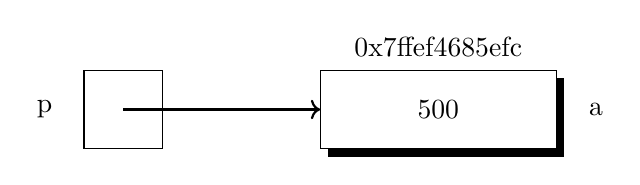
\begin{tikzpicture}
			% Draw the first rectangle
			\draw (4,0) rectangle (5,1);
			\node at (3.5,0.5) {p};
			
			% Draw the arrow
			\draw[->, thick] (4.5,0.5) -- (7,0.5);
			%\node at (6,0.7){p = \&a};
			
			% Draw the second rectangle
			\draw (7,0) rectangle (10,1);
			\node at (8.5,0.5) {500};
			\node at (8.5,1.3) {0x7ffef4685efc};
			\node at (10.5,0.5) {a};
			\fill[black] (7.1,0) rectangle (10.1,-0.1);
			\fill[black] (10,0) rectangle (10.1,0.9);
		\end{tikzpicture}
	\end{center}


	At last after \codebox{a = 98}:
	
	
	\begin{center}
		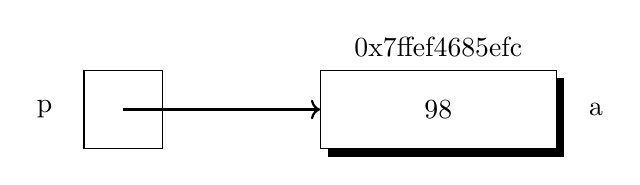
\begin{tikzpicture}
			% Draw the first rectangle
			\draw (4,0) rectangle (5,1);
			\node at (3.5,0.5) {p};
			
			% Draw the arrow
			\draw[->, thick] (4.5,0.5) -- (7,0.5);
			%\node at (6,0.7){p = \&a};
			
			% Draw the second rectangle
			\draw (7,0) rectangle (10,1);
			\node at (8.5,0.5) {98};
			\node at (8.5,1.3) {0x7ffef4685efc};
			\node at (10.5,0.5) {a};
			\fill[black] (7.1,0) rectangle (10.1,-0.1);
			\fill[black] (10,0) rectangle (10.1,0.9);
		\end{tikzpicture}
	\end{center}


	It is important that the address \codebox{0x7ffef4685efc} was not changed during the whole time, since we changed the value saved in the same location of the memory. Doesn't make sense right!? I know I have been there! Let's try another example:
	
	\begin{lstlisting}
		#include <stdio.h>
		
		int main() {
			int a, b, *p1, *p2;
			
			printf("The initial values:\n");
			printf("a=%d\n", a);
			printf("b=%d\n", b);
			printf("The address of a is: %p\n", &a);
			printf("The address of b is: %p\n", &b);
			printf("The address p1 is: %p\n", p1);
			printf("The address p2 is: %p\n", p2);
			printf("\n");
			
			p1 = &a;
			p2 = p1;
			printf("Result after p1 = &a and p2 = p1:\n");
			printf("Value of *p1: %d\n", *p1);
			printf("Value of *p2: %d\n", *p2);
			printf("Value of a: %d\n", a);
			printf("The address p1 is: %p\n", p1);
			printf("The address p2 is: %p\n", p2);
			printf("\n");
			
			*p1 = 1;
			printf("Step 1, after *p1 = 1:\n");
			printf("Value of *p1: %d\n", *p1);
			printf("Value of *p2: %d\n", *p2);
			printf("Value of a: %d\n", a);
			printf("The address p1 is: %p\n", p1);
			printf("The address p2 is: %p\n", p2);
			printf("\n");
			
			*p2 = 2;
			printf("Step 2, after *p2 = 2;\n");
			printf("Value of *p1: %d\n", *p1); // Output: 2
			printf("Value of *p2: %d\n", *p2); // Output: 2
			printf("Value of a: %d\n", a);	   // Output: 2
			printf("The address p1 is: %p\n", p1);
			printf("The address p2 is: %p\n", p2);
		}
	\end{lstlisting}
	
	
	In the first part, \codebox{p1} and \codebox{p2} are declared as integer pointers. \codebox{p1} is set to point to the address of variable \codebox{a}. Then \codebox{p2} is assigned the value of \codebox{p1}. Now both \codebox{p1} and \codebox{p2} point to the address of \codebox{a}, and the value of \codebox{a} becomes 1.
	
	Next, \codebox{*p2} is modified to 2. Since \codebox{p2} is pointing to the same address as \codebox{p1}, both \codebox{*p1} and \codebox{*p2} change to 2, and the value of a also becomes 2. The output in \textbf{my computer} is:
	
	
	\begin{mdframed}[style=myboxstyleTerminal1]
		\begin{verbatim}
			The initial values:
			a=-1188484519
			b=32767
			The address of a is: 0x7fffb9292400
			The address of b is: 0x7fffb9292404
			The address p1 is: 0x64
			The address p2 is: 0x1000
			
			Result after p1 = &a and p2 = p1:
			Value of *p1: -1188484519
			Value of *p2: -1188484519
			Value of a: -1188484519
			The address p1 is: 0x7fffb9292400
			The address p2 is: 0x7fffb9292400
			
			Step 1, after *p1 = 1:
			Value of *p1: 1
			Value of *p2: 1
			Value of a: 1
			The address p1 is: 0x7fffb9292400
			The address p2 is: 0x7fffb9292400
			
			Step 2, after *p2 = 2;
			Value of *p1: 2
			Value of *p2: 2
			Value of a: 2
			The address p1 is: 0x7fffb9292400
			The address p2 is: 0x7fffb9292400
		\end{verbatim}
	\end{mdframed}
	
	Let's go step by steps through schematic process! At the beginning \codebox{a} and \codebox{b} integers were declared without initialization. The same as \codebox{p1} and \codebox{p2} pointers. After \codebox{p1=\&a}, \codebox{p1} will point at the the address of \codebox{a}. Using \codebox{p1=p2}, \codebox{p2} will point at the same address (\codebox{\&a}) that \codebox{p1} is pointing at:
	
	\begin{center}
		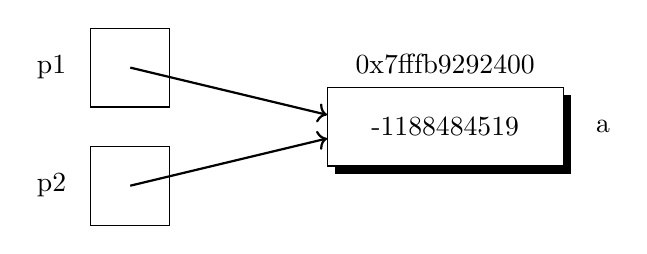
\begin{tikzpicture}
			% Draw the first rectangle
			\draw (4,0) rectangle (5,1);
			\node at (3.5,0.5) {p2};
			
			% Draw the second rectangle
			\draw (4,1.5) rectangle (5,2.5);
			\node at (3.5,2) {p1};
			
			% Draw the arrow
			\draw[->, thick] (4.5,2.0) -- (7,1.4);
			\draw[->, thick] (4.5,0.5) -- (7,1.1);
			
			
			% Draw the 3rd rectangle
			\draw (7,0.75) rectangle (10,1.75);
			\node at (8.5,1.25) {-1188484519};
			\node at (8.5,2.05) {0x7fffb9292400};
			\node at (10.5,1.25) {a};
			\fill[black] (7.1,0.75) rectangle (10.1,0.65);
			\fill[black] (10,0.75) rectangle (10.1,1.65);

		\end{tikzpicture}
	\end{center}
	
	By \codebox{*p1 = 1} we are changing the value saved in \codebox{p1} address which is the same as \codebox{p2} and \codebox{\&a}:
	
	\begin{center}
		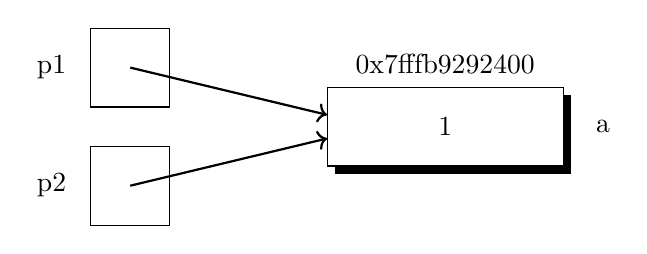
\begin{tikzpicture}
			% Draw the first rectangle
			\draw (4,0) rectangle (5,1);
			\node at (3.5,0.5) {p2};
			
			% Draw the second rectangle
			\draw (4,1.5) rectangle (5,2.5);
			\node at (3.5,2) {p1};
			
			% Draw the arrow
			\draw[->, thick] (4.5,2.0) -- (7,1.4);
			\draw[->, thick] (4.5,0.5) -- (7,1.1);
			
			
			% Draw the 3rd rectangle
			\draw (7,0.75) rectangle (10,1.75);
			\node at (8.5,1.25) {1};
			\node at (8.5,2.05) {0x7fffb9292400};
			\node at (10.5,1.25) {a};
			\fill[black] (7.1,0.75) rectangle (10.1,0.65);
			\fill[black] (10,0.75) rectangle (10.1,1.65);
			
		\end{tikzpicture}
	\end{center}
	
	Like it was said, \codebox{p2} is pointing at the same address, so we can change the value saved in this address using \codebox{*p2=2}:
	
	\begin{center}
		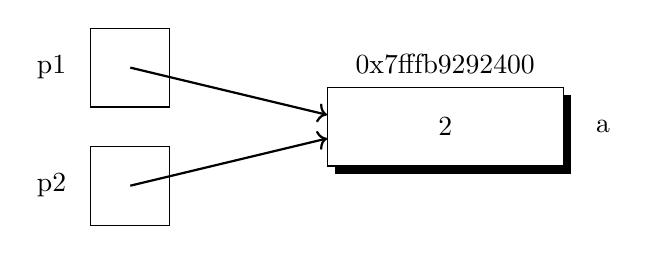
\begin{tikzpicture}
			% Draw the first rectangle
			\draw (4,0) rectangle (5,1);
			\node at (3.5,0.5) {p2};
			
			% Draw the second rectangle
			\draw (4,1.5) rectangle (5,2.5);
			\node at (3.5,2) {p1};
			
			% Draw the arrow
			\draw[->, thick] (4.5,2.0) -- (7,1.4);
			\draw[->, thick] (4.5,0.5) -- (7,1.1);
			
			
			% Draw the 3rd rectangle
			\draw (7,0.75) rectangle (10,1.75);
			\node at (8.5,1.25) {2};
			\node at (8.5,2.05) {0x7fffb9292400};
			\node at (10.5,1.25) {a};
			\fill[black] (7.1,0.75) rectangle (10.1,0.65);
			\fill[black] (10,0.75) rectangle (10.1,1.65);
			
		\end{tikzpicture}
	\end{center}
	
	
	
	\begin{tcolorbox}[myboxstyle]
		
		{\Large \textbf{\textcolor{cherry}{Warning!}}} Do not confuse \codebox{p1 = p2} with \codebox{*p1 = *p2}. Take a look at the following example and compare it with the previous one!
		
	\end{tcolorbox}
	
	\begin{lstlisting}
		#include <stdio.h>
		
		int main() {
			int x = 10, y = 20, *p1, *p2;
			p1 = &x;
			p2 = &y;
			printf("The initial values:\n");
			printf("x=%d\n", x);
			printf("y=%d\n", y);
			printf("The address of x is: %p\n", &x);
			printf("The address of y is: %p\n", &y);
			printf("The address p1 is: %p\n", p1);
			printf("The address p2 is: %p\n", p2);
			printf("\n");
			
			*p1 = *p2;
			printf("After *p1 = *p2:\n");
			printf("x=%d\n", x);
			printf("y=%d\n", y);
			printf("Value at address pointed by p1: %d\n", *p1); 
			printf("Value at address pointed by p2: %d\n", *p2);
			
			printf("The address of x is: %p\n", &x);
			printf("The address of y is: %p\n", &y);
			printf("The address p1: %p\n", p1);			 
			printf("The address p2: %p\n", p2);			 
		}
	\end{lstlisting}
	
	In this example, new integer variables \codebox{x} and \codebox{y} are declared, and \codebox{p1} is set to point to the address of \codebox{x}, while \codebox{p2} is set to point to the address of \codebox{y}. Then, the addresses and values stored at those addresses are printed.
	
	Finally, \codebox{*p1} is assigned the value of \codebox{*p2}. This means the value stored at the address pointed by \codebox{p2} (value of \codebox{y}) is \textbf{copied} to the address pointed by \codebox{p1} (value of \codebox{x}). After this step, both \codebox{*p1} and \codebox{*p2} become 20, and the addresses of \codebox{p1} and \codebox{p2} remain unchanged.
	
	\begin{mdframed}[style=myboxstyleTerminal1]
		\begin{verbatim}
			The initial values:
			x=10
			y=20
			The address of x is: 0x7ffe112ad7a0
			The address of y is: 0x7ffe112ad7a4
			The address p1 is: 0x7ffe112ad7a0
			The address p2 is: 0x7ffe112ad7a4
			
			After *p1 = *p2:
			x=20
			y=20
			Value at address pointed by p1: 20
			Value at address pointed by p2: 20
			The address of x is: 0x7ffe112ad7a0
			The address of y is: 0x7ffe112ad7a4
			The address p1: 0x7ffe112ad7a0
			The address p2: 0x7ffe112ad7a4
		\end{verbatim}
	\end{mdframed}
	
	At the first place we used \codebox{p1} and \codebox{p2} to point at the addresses of saved variables \codebox{x} and \codebox{y}, using \codebox{p1 = \&x} and \codebox{p2 = \&y}:
	
	\begin{center}
		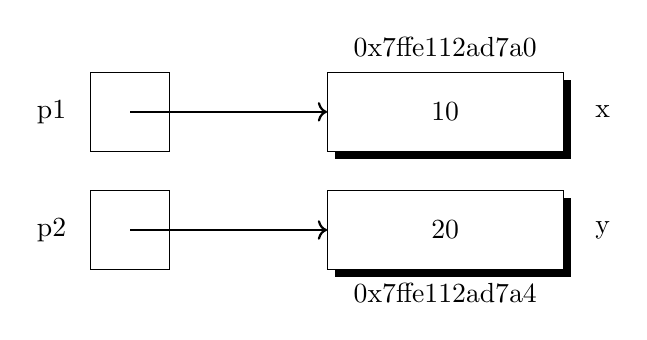
\begin{tikzpicture}
			% Draw the first rectangle
			\draw (4,0) rectangle (5,1);
			\node at (3.5,0.5) {p2};
			
			% Draw the second rectangle
			\draw (4,1.5) rectangle (5,2.5);
			\node at (3.5,2) {p1};
			
			% Draw the arrow
			\draw[->, thick] (4.5,0.5) -- (7,0.5);
			\draw[->, thick] (4.5,2.0) -- (7,2.0);
			
			
			\draw (7,0) rectangle (10,1);
			\node at (8.5,0.5) {20};
			\node at (8.5,-0.3) {0x7ffe112ad7a4};
			\node at (10.5,0.5) {y};
			\fill[black] (7.1,0) rectangle (10.1,-0.1);
			\fill[black] (10,0) rectangle (10.1,0.9);
			
			\draw (7,1.5) rectangle (10,2.5);
			\node at (8.5,2) {10};
			\node at (8.5,2.83) {0x7ffe112ad7a0};
			\node at (10.5,2) {x};
			\fill[black] (7.1,1.5) rectangle (10.1,1.4);
			\fill[black] (10,1.5) rectangle (10.1,2.4);

		\end{tikzpicture}
	\end{center}


	After \codebox{*p1 = *p2}, we are saying the value saved in the address \codebox{p1} (accessible by \codebox{*p1}) must be equal to the value saved in the address \codebox{p2}:
	
	\begin{center}
		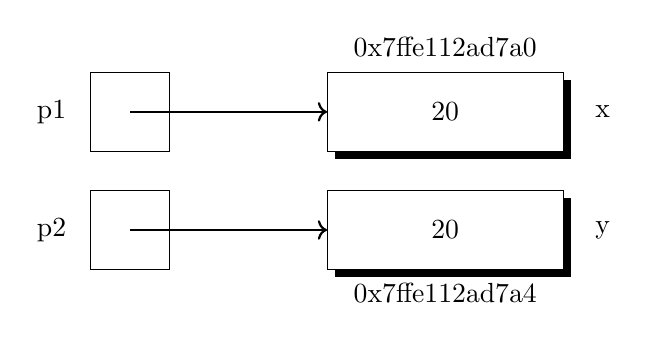
\begin{tikzpicture}
			% Draw the first rectangle
			\draw (4,0) rectangle (5,1);
			\node at (3.5,0.5) {p2};
			
			% Draw the second rectangle
			\draw (4,1.5) rectangle (5,2.5);
			\node at (3.5,2) {p1};
			
			% Draw the arrow
			\draw[->, thick] (4.5,0.5) -- (7,0.5);
			\draw[->, thick] (4.5,2.0) -- (7,2.0);
			
			
			\draw (7,0) rectangle (10,1);
			\node at (8.5,0.5) {20};
			\node at (8.5,-0.3) {0x7ffe112ad7a4};
			\node at (10.5,0.5) {y};
			\fill[black] (7.1,0) rectangle (10.1,-0.1);
			\fill[black] (10,0) rectangle (10.1,0.9);
			
			\draw (7,1.5) rectangle (10,2.5);
			\node at (8.5,2) {20};
			\node at (8.5,2.83) {0x7ffe112ad7a0};
			\node at (10.5,2) {x};
			\fill[black] (7.1,1.5) rectangle (10.1,1.4);
			\fill[black] (10,1.5) rectangle (10.1,2.4);
			
		\end{tikzpicture}
	\end{center}
	
	
	\begin{tcolorbox}[myboxstyle]
		
		{\Large \textbf{\textcolor{cherry}{Let's take a break!}}} Are you still following? Good! Why we are doing this? \textbf{why we need pointers?} Pointers are used when passing variables to functions for several reasons:
		
		\begin{itemize}
			\item \textbf{Passing by Reference}: In C, function arguments are typically passed by value, which means a copy of the argument is made and passed to the function. However, when we need to modify the original variable inside the function and reflect those changes outside the function, we use pointers. By passing the address of the variable (a pointer) to the function, the function can directly modify the original variable in memory, not just a copy of it.
			\item \textbf{Memory Efficiency}: When dealing with large data structures or arrays, passing them by value can be memory-intensive because it creates copies. By passing pointers to these structures or arrays, we avoid unnecessary memory consumption and improve the program's efficiency.
			\item \textbf{Dynamic Memory Allocation}: Pointers are essential when working with dynamically allocated memory. Functions that allocate memory (e.g., using malloc) return pointers to the allocated memory, allowing us to access and manage the allocated memory effectively (\hyperref[sec:allocation]{\textcolor{orange!80!black}{Dynamic Memory Allocation}}).
			\item \textbf{Sharing Data Across Functions}: Pointers enable sharing data between different functions without the need for global variables. Functions can access and modify the same data by using pointers, promoting modularity and encapsulation.
			\item \textbf{Function Return Multiple Values}: C functions can return only a single value, but using pointers as function arguments, we can return multiple values from a function.
			\item \textbf{Data Structure}s: Pointers are widely used in creating complex data structures like linked lists, trees, and graphs, where each element points to the next or previous element.
		\end{itemize}
			
	\end{tcolorbox}
	
	
	
	
	
	
	\subsection{Constant Pointers}
	
	Like any other data type, pointers can also be defined as constant using the const keyword. When a pointer is defined as constant, it means that the memory address it points to cannot be changed, making it a constant pointer. Let's consider an example to illustrate the concepts. This example is taken from \href{https://baraksh.com/CSE701/notes.php#memory-addresses-and-the-stack}{Prof. Barak Shoshany}:
	
	\begin{lstlisting}
		#include <stdio.h>
		
		int main() {
			int variable1 = 10;
			double variable2 = 3.14;
			
			const int const1 = 20;
			const double const2 = 2.71;
			
			int *variable_pointer_to_variable = &variable1;  
			int *const const_pointer_to_variable = &variable2; 
			
			const int *variable_pointer_to_const = &const1;    
			const int *const const_pointer_to_const = &const2; 
			
			// Allowed: var is not const, so can be changed.
			variable1 = 12; 
			// Not Allowed: con is const, so cannot be changed.
			const1 = 30;
			
			// Allowed: pointer itself is not const, so can be changed.
			variable_pointer_to_variable = &variable2; 
			// Allowed: variable pointed to is not const, so can be changed.
			*variable_pointer_to_variable = 30;         
			
			// Not Allowed: pointer itself is const, so cannot be changed.
			const_pointer_to_variable = &variable1; 
			// Allowed: variable pointed to is not const, so can be changed.
			*const_pointer_to_variable = 30;         
			
			// Allowed: pointer itself is not const, so can be changed.
			variable_pointer_to_const = &const2; 
			// Not Allowed: variable pointed to is const, so cannot be changed.
			*variable_pointer_to_const = 50;         
			
			// Not Allowed: pointer itself is const, so cannot be changed.
			const_pointer_to_const = &const1; 
			// Not Allowed: variable pointed to is const, so cannot be changed.
			*const_pointer_to_const = 30;         
		}
	\end{lstlisting}
	
	\begin{itemize}
		\item \codebox{type <variable>}: This declares a variable of type \codebox{type}. The value of the variable can be modified throughout its lifetime!
		
		\item \codebox{const type <variable>}: This declares a constant variable of type \codebox{type}. The value of the variable cannot be modified after it is initialized.
		
		\item \codebox{type *<pointer>}: This declares a pointer variable of type \codebox{type*}. The pointer can store the memory address of a variable of type \codebox{type}, and the value pointed to by the pointer can be modified.
		
		\item \codebox{type *const <pointer>}: This declares a constant pointer variable of type \codebox{type*}. The memory address stored in the pointer cannot be modified after it is initialized, but the value pointed to by the pointer can be modified.
		
		\item \codebox{const type *<pointer>}: This declares a pointer variable of type \codebox{const type*}. The pointer can store the memory address of a variable of type \codebox{const type}, and the value pointed to by the pointer cannot be modified.
		
		\item \codebox{const type *const <pointer>}: This declares a constant pointer variable of type \codebox{const type*}. The memory address stored in the pointer cannot be modified after it is initialized, and the value pointed to by the pointer cannot be modified.
	\end{itemize}
	
	
	\begin{tcolorbox}[myboxstyle]
		
		{\Large \textbf{\textcolor{cherry}{Tips!}}} There is no difference between:
		
		\codebox{const int *variable\_pointer\_to\_const}
		
		and
		
		\codebox{int const *variable\_pointer\_to\_const}
		
		In both cases, \codebox{const} is before \codebox{*}, indicating that the variable itself is constant NOT the pointer.
	\end{tcolorbox}
	
	
	
	
	
	
	
	
	\subsection{Pointers and Arrays}
	
	In C, arrays have a close relationship with pointers. When an array is declared, it automatically creates a pointer that points to the memory location of its first element. This means that arrays are essentially a contiguous block of memory, and each element in the array can be accessed using pointer arithmetic. Here's a C code that demonstrates initializing an array, printing out the address for each element, and printing the value of each element:
	
	\begin{lstlisting}
		#include <stdio.h>
		
		int main() {
			int arr[] = {10, 20, 30, 40, 50};  // Initializing an array with values
			
			// Printing the address and value of each element in the array
			for (int i = 0; i < 5; i++) {
				printf("arr[%d] = %d with address %p\n", i, arr[i], &arr[i]);
			}
		}
	\end{lstlisting}
	
	In this example, we declare an array \codebox{arr} with five elements. We then use a loop to iterate through each element of the array. By using the \codebox{\&} operator, we can get the address of each element and print it using \codebox{\%p} format specifier. Additionally, we print the value of each element using \codebox{\%d} format specifier. The output shows that each element of the array is stored at a unique memory address, and we can access their values using the pointers to those addresses.
	
	
	
	
	
	
	
	\subsubsection*{Array of Characters}
	
	In C, strings are represented as arrays of characters, where each character represents a single element of the string. A C string is terminated with a null character \codebox{'\textbackslash0'}, which indicates the end of the string. Therefore, a string of length n requires an array of n+1 characters, with the last element being the null character. Both of the following statements are valid ways to initialize a string in C:
	
	\begin{lstlisting}
		char date[] = "July 24"; // Initializing using an array
		char *date = "July 24";  // Initializing using a pointer
	\end{lstlisting}
	
	In the first example, date is declared as an array of characters, and the compiler automatically determines the size of the array based on the length of the string literal "July 24". Here is how \codebox{date} will look like:
	
	\begin{center}
		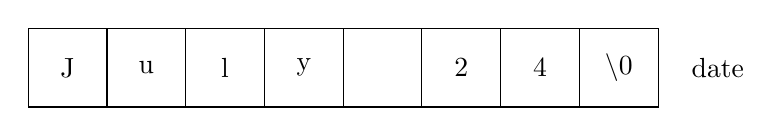
\begin{tikzpicture}
			% Define the side length of the squares
			\newcommand{\sideLength}{1cm}
			
			% Draw the squares and the characters
			\foreach \char [count=\i] in {J,u,l,y, ,2,4,\textbackslash0} {
				\node[draw, minimum size=\sideLength, inner sep=0pt] at (\i*\sideLength-\sideLength/2, 0) {\char};
				\xdef\lasti{\i} % Store the value of the last index
			}
			
			% Calculate the position of the last square
			\pgfmathsetmacro{\lastx}{\lasti*\sideLength-\sideLength/2}
			
			% Draw the note to the right of the last square
			\node[right=-0.2cm] at (\lastx+\sideLength, 0) {date};
			
		\end{tikzpicture}
	\end{center}
	
	In the second example, date is declared as a pointer to a character, and it is assigned the address of the string literal "July 24". Note that in this case, the size of the array is not explicitly specified, as the compiler automatically allocates the appropriate memory to store the string literal. To find the last element of an array you can use a the following code:
	
	\begin{lstlisting}
		#include <stdio.h>
		
		// Function to find the end of a string using a pointer
		void findEndOfString(const char *str) {
			while (*str != '\0') {
				str++; // Move the pointer to the next character
			}
			// Print the last character of the string
			printf("End of string: %c\n", *(str - 1)); 
		}
		
		int main() {
			// Single string
			const char myString[] = "Hello, this is a test string.";
			
			// Send the string as a pointer to the function to find the end
			findEndOfString(myString);
		}
	\end{lstlisting}
	
	Or if you want to find the length of a string something like \codebox{strlen} function you can use the following code:
	
	\begin{lstlisting}
		#include <stdio.h>
		
		// Function to find the end of a string using a pointer with a for loop
		int findEndOfString(const char *str) {
			int n;
			for (n = 0; *str != '\0'; str++) {
				n++;
			}
			return n; // Return the last character of the string
		}
		
		int main() {
			// Single string
			const char myString[] = "Hello, this is a test string.";
			
			// Send the string as a pointer to the function to find the end
			int lastCharacter = findEndOfString(myString);
			printf("End of string: %d\n", lastCharacter);
			
			// this one also counts the last character which is a null character '\0'
			int length_str = sizeof(myString)/sizeof(myString[0]);
			printf("Size of string: %d\n", length_str);
		}
	\end{lstlisting}
	
	Both codes use \codebox{`\textbackslash0`} to find the last character. I can do the same by using an array notation for function parameter:
	
	\begin{lstlisting}
		#include <stdio.h>
		
		// Function to find the end of a string using an array
		int findEndOfString(const char str[]) {
			int n;
			for (n = 0; str[n] != '\0'; n++) {
				// Loop until the null terminator is found
				// it was better to use while
				// I did to make it similar to the previous version
			}
			return n - 1; // Return the index of the last character in the string
		}
		
		int main() {
			// Single string
			const char myString[] = "Hello, this is a test string.";
			
			// Send the string as an array to the function to find the end
			int lastCharacter = findEndOfString(myString);
			
			printf("End of string: %c\n", myString[lastCharacter]);
		}
	\end{lstlisting}
	
	The difference between \codebox{(const char str[])} and \codebox{(const char *str)} lies in how the function can access the characters of the string.
	
	\codebox{(const char str[])}: This is an array notation for function parameters, also known as array notation for passing strings. When you pass a string as \codebox{const char str[]}, the function treats it as an array of characters. Inside the function, you can access the characters of the string using array indexing \codebox{(str[n])}. The compiler will automatically adjust the pointer to the first element of the array, so you can use it as if it were a regular array.
	
	\codebox{(const char *str)}: This is a pointer notation for function parameters, also known as pointer notation for passing strings. When you pass a string as \codebox{const char *str}, the function treats it as a pointer to the first character of the string. Inside the function, you can access the characters of the string using pointer arithmetic (\codebox{*(str + n)} or \codebox{str[n]}). In this case, you explicitly use pointer arithmetic to traverse the characters.
	
	Both notations allow you to pass strings to functions, and both versions of the function will work correctly to find the end of the string. In both the pointers are sent and there will not be another copy of array (waste of memory)in the function. You can used \textbf{GDB} to print out the addresses. The choice between array notation and pointer notation is mostly a matter of preference and coding style. Array notation may be more intuitive and familiar to some developers, while pointer notation may be preferred for its similarity to working with arrays and dynamic memory. Ultimately, both notations achieve the same goal of accessing the characters of the string within the function.
	
	Let's discuss the \codebox{scanf} function and why we use \codebox{\&} before the string variable when reading input:
	
	\begin{lstlisting}
		char str[50];
		scanf("%s", &str);
	\end{lstlisting}
	
	The \codebox{scanf} function is used for reading input from the user. When using\codebox{scanf} to read a string, you need to provide the address of the variable where the string will be stored. Since str is an array of characters, it already represents a memory address. However, when using \codebox{scanf}, you need to \textbf{explicitly} specify the address using the \codebox{\&} (address-of) operator.
	
	In this case, \codebox{\&str} represents the address of the first element of the \codebox{str} array, which is the starting address where the string entered by the user will be stored. The \codebox{scanf} function reads characters from the standard input and stores them in the memory pointed to by \codebox{\&str}, until it encounters a whitespace character (space, tab, or newline), effectively reading a single word (no spaces) as input. The null character \codebox{'\textbackslash0'} is automatically appended at the end of the input, ensuring that the array \codebox{str} is properly terminated as a C string.
	
	
	
	
	
	\subsubsection*{Array of Strings}
	
	
	In C, an array of strings is a two-dimensional array of characters, where each element of the array represents a string. Each string is a sequence of characters terminated by a null character \codebox{'\textbackslash0'}. The array is organized in rows, where each row represents a separate string. Since each array might have combination of long and short stings we need to save them in a two dimensional array with different length in each row, which is called \textbf{ragged array}.
	
	
	\begin{lstlisting}[basicstyle=\footnotesize]
		#include <stdio.h>
		
		int main()
		{
			// Ragged array of strings
			char names[][11] = {"Anne-Marie", "Anna", "Mahmoud", "Kian", "Raouf", "Nikki"};
			
			// Accessing and printing the elements and their lengths
			for (int i = 0; i < 6; i++)
			{
				int length = 0;
				while (names[i][length] != '\0'){
					length++;
				}
				// OR we can use `int length = strlen(names[i]);` from `<string.h>`
				// `int length = sizeof(names[i])/sizeof(names[i][0]) - 1; ` will not work why?
				
				// `length+1` in `names[i][length+1]` to skip `\0`
				printf("Name %d: %s (Length: %d) - After '\\0': '%c'\n", i + 1, names[i], length, names[i][length+1]);
			}
		}
	\end{lstlisting}
	
	In this example the size of stings is between 4 to 10, and this is how it is saved:
	
	
	
	
	\begin{center}
		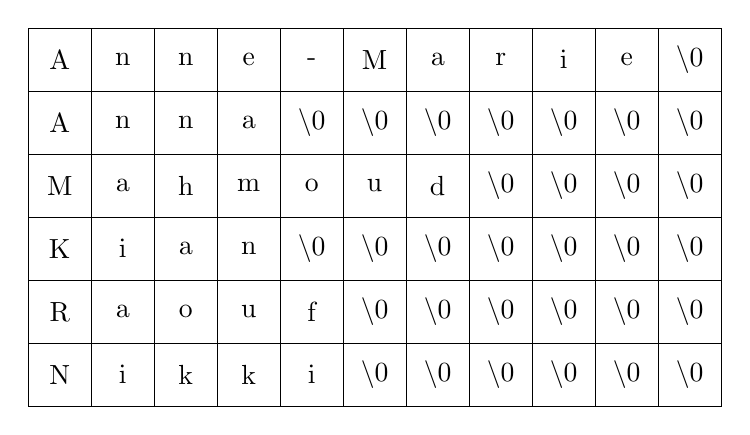
\begin{tikzpicture}
			% Define the side length of the squares
			\newcommand{\sideLength}{0.8cm}
			% Define the number of rows and columns
			\newcommand{\numRows}{6}
			\newcommand{\numCols}{11}
			
			% Loop through rows and columns to draw squares and notes
			\foreach \row in {1,...,\numRows} {
				\ifnum\row=1
				\foreach \col [count=\i] in {A,n,n,e,-,M,a,r,i,e,\textbackslash0} {
					\node[draw, minimum size=\sideLength, inner sep=0pt] at (\i*\sideLength-\sideLength/2, -\row*\sideLength+\sideLength/2) {\col};
				}
				\fi
				\ifnum\row=2
				\foreach \col [count=\i] in {A,n,n,a,\textbackslash0,\textbackslash0,\textbackslash0,\textbackslash0,\textbackslash0,\textbackslash0,\textbackslash0} {
					\node[draw, minimum size=\sideLength, inner sep=0pt] at (\i*\sideLength-\sideLength/2, -\row*\sideLength+\sideLength/2) {\col};
				}
				\fi
				\ifnum\row=3
				\foreach \col [count=\i] in {M,a,h,m,o,u,d,\textbackslash0,\textbackslash0,\textbackslash0,\textbackslash0} {
					\node[draw, minimum size=\sideLength, inner sep=0pt] at (\i*\sideLength-\sideLength/2, -\row*\sideLength+\sideLength/2) {\col};
				}
				\fi
				\ifnum\row=4
				\foreach \col [count=\i] in {K,i,a,n,\textbackslash0,\textbackslash0,\textbackslash0,\textbackslash0,\textbackslash0,\textbackslash0,\textbackslash0} {
					\node[draw, minimum size=\sideLength, inner sep=0pt] at (\i*\sideLength-\sideLength/2, -\row*\sideLength+\sideLength/2) {\col};
				}
				\fi
				\ifnum\row=5
				\foreach \col [count=\i] in {R,a,o,u,f,\textbackslash0,\textbackslash0,\textbackslash0,\textbackslash0,\textbackslash0,\textbackslash0} {
					\node[draw, minimum size=\sideLength, inner sep=0pt] at (\i*\sideLength-\sideLength/2, -\row*\sideLength+\sideLength/2) {\col};
				}
				\fi
				\ifnum\row=6
				\foreach \col [count=\i] in {N,i,k,k,i,\textbackslash0,\textbackslash0,\textbackslash0,\textbackslash0,\textbackslash0,\textbackslash0} {
					\node[draw, minimum size=\sideLength, inner sep=0pt] at (\i*\sideLength-\sideLength/2, -\row*\sideLength+\sideLength/2) {\col};
				}
				\fi
			}
		\end{tikzpicture}
	\end{center}
	
	
	
	The given code is not ragged because it uses a 2-dimensional array to store the strings. In a ragged array, the array elements are pointers, and each element can point to an array of different sizes. In the provided code, names is a 2-dimensional array of characters, and all the strings have a fixed length of 11 characters (including the null-terminating character \codebox{'\textbackslash0'}). The output:
	
	\begin{mdframed}[style=myboxstyleTerminal1]
		\begin{verbatim}
			Name 1: Anne-Marie (Length: 10) - After '\0': 'A'
			Name 2: Anna (Length: 4) - After '\0': ''
			Name 3: Mahmoud (Length: 7) - After '\0': ''
			Name 4: Kian (Length: 4) - After '\0': ''
			Name 5: Raouf (Length: 5) - After '\0': ''
			Name 6: Nikki (Length: 5) - After '\0': ''
		\end{verbatim}
	\end{mdframed}
	
	
	
	A \textbf{ragged array} is a two-dimensional array where the rows can have different sizes (different number of elements). In contrast, a regular two-dimensional array has fixed sizes for all rows and columns. Ragged arrays are useful when you have data with varying sizes or when you want to optimize memory usage. For example, if you have a table of data with different lengths of rows, a ragged array can efficiently store this data without wasting memory on empty elements. For example:
	
	\begin{lstlisting}[basicstyle=\footnotesize]
		#include <stdio.h>
		#include <string.h>
		
		int main()
		{
			// Ragged array of strings
			char *names[] = {"Anne-Marie", "Anna", "Mahmoud", "Kian", "Raouf", "Nikki"};
			
			// Accessing and printing the elements and their lengths
			for (int i = 0; i < 6; i++)
			{
				int length = strlen(names[i]);
				
				// `length+1` in `names[i][length+1]` to skill `\0`
				printf("Name %d: %s (Length: %d) - After '\\0': '%c'\n", i + 1, names[i], length, names[i][length+1]);
			}
		}
	\end{lstlisting}
	
	Here's an explanation of the code:
	
	\codebox{char *names[]}: This declares an array of pointers to characters. Each element of names is a pointer that can point to the first character of a string.
	
	\codebox{{"Anne-Marie", "Anna", "Mahmoud", "Kian", "Raouf", "Nikki"};}: This initializes the names array with string literals. Each string literal is stored in a separate memory location, and the pointers in the names array point to the first character of each string. The for loop iterates through each element of the names array.
	
	Inside the loop, length is initialized to 0. The while loop is used to find the length of each string in the names array. It continues until it reaches the null-terminating character \codebox{'\textbackslash0'}, which marks the end of the string.
	
	After finding the length of the string, the code prints the details using \codebox{printf}. This line prints the information for each string. It displays the name's index, the string itself, its length, and the character that appears after the null-terminating character. Note that \codebox{names[i][length]} is used to check the character after \codebox{'\textbackslash0'}! This is how the array is save while each pointer to the row will point only to the first element of the row (\codebox{*names[i]}).
	
	\begin{center}
		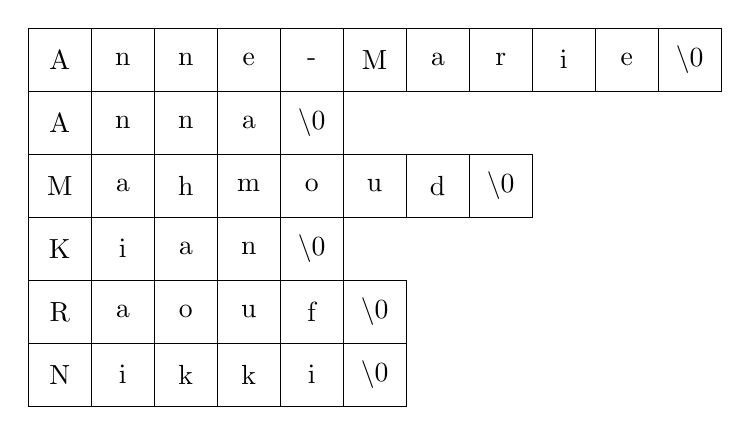
\begin{tikzpicture}
			% Define the side length of the squares
			\newcommand{\sideLength}{0.8cm}
			% Define the number of rows
			\newcommand{\numRows}{6}
			
			% Loop through rows and columns to draw squares and notes
			\foreach \row in {1,...,\numRows} {
				\ifnum\row=1
				\newcommand{\numCols}{11}
				\foreach \col [count=\i] in {A,n,n,e,-,M,a,r,i,e,\textbackslash0} {
					\node[draw, minimum size=\sideLength, inner sep=0pt] at (\i*\sideLength-\sideLength/2, -\row*\sideLength+\sideLength/2) {\col};
				}
				\fi
				\ifnum\row=2
				\newcommand{\numCols}{5}
				\foreach \col [count=\i] in {A,n,n,a,\textbackslash0} {
					\node[draw, minimum size=\sideLength, inner sep=0pt] at (\i*\sideLength-\sideLength/2, -\row*\sideLength+\sideLength/2) {\col};
				}
				\fi
				\ifnum\row=3
				\newcommand{\numCols}{8}
				\foreach \col [count=\i] in {M,a,h,m,o,u,d,\textbackslash0} {
					\node[draw, minimum size=\sideLength, inner sep=0pt] at (\i*\sideLength-\sideLength/2, -\row*\sideLength+\sideLength/2) {\col};
				}
				\fi
				\ifnum\row=4
				\newcommand{\numCols}{5}
				\foreach \col [count=\i] in {K,i,a,n,\textbackslash0} {
					\node[draw, minimum size=\sideLength, inner sep=0pt] at (\i*\sideLength-\sideLength/2, -\row*\sideLength+\sideLength/2) {\col};
				}
				\fi
				\ifnum\row=5
				\newcommand{\numCols}{6}
				\foreach \col [count=\i] in {R,a,o,u,f,\textbackslash0} {
					\node[draw, minimum size=\sideLength, inner sep=0pt] at (\i*\sideLength-\sideLength/2, -\row*\sideLength+\sideLength/2) {\col};
				}
				\fi
				\ifnum\row=6
				\newcommand{\numCols}{6}
				\foreach \col [count=\i] in {N,i,k,k,i,\textbackslash0} {
					\node[draw, minimum size=\sideLength, inner sep=0pt] at (\i*\sideLength-\sideLength/2, -\row*\sideLength+\sideLength/2) {\col};
				}
				\fi
			}
		\end{tikzpicture}
	\end{center}
	
	
	
	This time the output is:
	
	\begin{mdframed}[style=myboxstyleTerminal1]
		\begin{verbatim}
			Name 1: Anne-Marie (Length: 10) - After '\0': 'A'
			Name 2: Anna (Length: 4) - After '\0': 'M'
			Name 3: Mahmoud (Length: 7) - After '\0': 'K'
			Name 4: Kian (Length: 4) - After '\0': 'R'
			Name 5: Raouf (Length: 5) - After '\0': 'N'
			Name 6: Nikki (Length: 5) - After '\0': ''
		\end{verbatim}
	\end{mdframed}
	
	The effects of using a ragged array are that the individual strings (sub-arrays) can have different lengths, making it more flexible in handling data with varying sizes. \textbf{Use GDB and print out the addresses to see the sequence}.
	
	
	
	The difference between the first code and this ragged array is that the ragged array code used a 1-dimensional array of pointers, and each pointer pointed to a separate memory location holding a string of different lengths. In contrast, the updated code uses a 2-dimensional array of characters, where each row represents a string with a fixed length. To see the effects of one dimensional array in ragged code, we can print out \codebox{names[i][length+1]} which is the character after null-terminating character. In the first one, it still prints out \codebox{''} (\codebox{'\textbackslash0'}). \textbf{But how we can pass a 2D array (array of strings) to a function?}
	
	

	
	
	
	
	
	\subsection{Pointers as Arguments of a Function}
	
	It was mentioned that one of the benefits of Pointers is \textbf{Passing by Reference}, allowing us to modify a variable in another scope. In Section \hyperref[sec:Scope in functions]{\textcolor{orange!80!black}{Variable Scope in Functions}}, we had a function \codebox{printNumber()} that declares a local variable number inside the function. We also have a variable \codebox{number} declared in the \codebox{main()} function. Let's modify the code to explain how using pointers can help us modify a value passed to a function.
	
	\begin{lstlisting}
		#include <stdio.h>
		
		void printNumber(int *ptr) {
			// Using a pointer to modify the value passed to the function
			*ptr = 10;
			
			printf("Number inside the function: %d\n", *ptr);
		}
		
		int main() {
			int number = 5;  // Variable declared inside the main function
			
			printf("Number inside the main function: %d\n", number);
			
			// Pass the address of 'number' to the function
			printNumber(&number);
			
			// The value of 'number' has been modified by the function
			printf("Number after the function call: %d\n", number);
		}
	\end{lstlisting}
	
	
	In this modified code, we have made the following changes:
	
	The function \codebox{printNumber()} now takes a pointer to an integer (\codebox{int *ptr)} as an argument instead of having a local variable. By passing the address of number to this function, we can access and modify the original number variable inside the \codebox{main()} function.
	
	Inside the \codebox{printNumber()} function, we use the pointer \codebox{ptr} to modify the value of number to 10. We do this by de-referencing the pointer using \codebox{*ptr}, which gives us access to the value stored at the address pointed to by the pointer.
	
	After the function call, we print the value of number again in the \codebox{main()} function. Since we passed the address of number to the \codebox{printNumber()} function and modified it using the pointer, the value of number has been changed to 10 even outside the \codebox{printNumber()} function. The result must be:
	
	\begin{mdframed}[style=myboxstyleTerminal1]
		\begin{verbatim}
			Number inside the main function: 5
			Number inside the function: 10
			Number after the function call: 10
		\end{verbatim}
	\end{mdframed}
	
	Using pointers allows us to directly access and modify the original variable's value inside the function, which can be helpful when we need to modify the value of a variable passed to a function. This is particularly useful when we want to achieve pass-by-reference behavior in C, as C functions are typically pass-by-value by default. Let's try another example. This C code passes a double value and pointers to a function, performs some calculations inside the function, and updates the values pointed to by the pointers:
	
	\begin{lstlisting}
		#include <stdio.h>
		
		void calculate(double num, double *square, double *cube) {
			
			// update the value stored at square pointer
			*square = num * num;
			
			// update the value stored at cube pointer
			*cube = num * num * num; 
		}
		
		int main() {
			// Initial value
			double number = 5.0;  
			
			// Variables to store the results
			double result_square, result_cube;  
			
			// Call the function to calculate the square and cube
			calculate(number, &result_square, &result_cube);
			
			// Print the results
			printf("Number: %.2f\n", number);
			printf("Square: %.2f\n", result_square);
			printf("Cube: %.2f\n", result_cube);
		}
	\end{lstlisting}
	
	Let's go through the code using GDB (LLDB). So compile the code with \codebox{-g}. Run the executable object with \codebox{gdb ./pedram} (lldb ./pedram). Define the following breakpoints. If you have copied the code with same format of spaces between lines, the numbering here must be the same as yours, otherwise you need to change the number mentioned here.
	
	\begin{itemize}
		\item \codebox{break 20} at \codebox{calculate(number, \&result\_square, \&result\_cube);} right before calling the function.
		\item \codebox{break 6} at \codebox{*square = num * num;} right before updating the value stored at the address pointed by pointer \codebox{square}.
		\item \codebox{break 9} at \codebox{*cube = num * num * num} before updating the value stored at the address pointed by pointer \codebox{cube}.
	\end{itemize}
	
	Enter \codebox{run} to start debugging the program. Follow the output in \textbf{my computer} line by line. \textbf{This is really important!}
	
	\begin{mdframed}[style=myboxstyleTerminal1]
		\begin{verbatim}
			Breakpoint 1, main () at pedram.c:20
			20          calculate(number, &result_square, &result_cube);
			$1 = 6.9533558070931648e-310
			(gdb) p result_cube
			$2 = 4.9406564584124654e-322
			(gdb) n
			Breakpoint 2, calculate (num=5, square=0x7fffffffbef0, cube=0x7fffffffbef8)
			6               *square = num * num;
			(gdb) p num
			$3 = 5
			(gdb) p square
			$4 = (double *) 0x7fffffffbef0
			(gdb) p cube 
			$5 = (double *) 0x7fffffffbef8
			(gdb) p *square
			$6 = 6.9533558070931648e-310
			(gdb) p *cube
			$7 = 4.9406564584124654e-322
			(gdb) n
			
			Breakpoint 3, calculate (num=5, square=0x7fffffffbef0, cube=0x7fffffffbef8)
			9           *cube = num * num * num; 
			(gdb) p square
			$8 = (double *) 0x7fffffffbef0
			(gdb) p *square
			$9 = 25
			(gdb) n
			10      }
			(gdb) p *cube
			$10 = 125
			(gdb) n
			main () at pedram.c:23
			23          printf("Number: %.2f\n", number);
			(gdb) p result_square
			$11 = 25
			(gdb) p result_cube
			$12 = 125
			(gdb) c
			Continuing.
			Number: 5.00
			Square: 25.00
			Cube: 125.00
			[Inferior 1 (process 95816) exited normally]
			(gdb) q 
		\end{verbatim}
	\end{mdframed}
	
	Let's go through it step by step:
	
	\begin{itemize}
		\item The program starts at \codebox{main()} on line 20. It halts at Breakpoint 1 on line 20, where the call to the \codebox{calculate()} function is about to be made.
		
		\item When we print the values of \codebox{result\_square} and \codebox{result\_cube}, GDB shows that their values are initially uninitialized and contain garbage values. The garbage values are displayed in scientific notation.
		
		\item We proceed with the program execution using \codebox{n} (next) command, and it reaches Breakpoint 2 inside the \codebox{calculate()} function.
		
		\item When we print the values of \codebox{num}, \codebox{square}, and \codebox{cube}, GDB shows the correct values of the arguments passed to the function. \codebox{num} is 5, and square and cube are pointers to \codebox{result\_square} and \codebox{result\_cube} in the \codebox{main()} function.
		
		\item Printing \codebox{*square} and \codebox{*cube} shows that they still contain the initial garbage values.
		
		\item We continue the execution using \codebox{n}, and it reaches Breakpoint 3 inside the \codebox{calculate()} function.
		
		\item After calculating the square and cube and updating the values using pointers, we print \codebox{*square} again, which now correctly shows 25, the square of \codebox{num}. Similarly, \codebox{*cube} correctly shows 125, the \codebox{cube} of \codebox{num}.
		
		\item We continue the execution using \codebox{n}, and it returns to \codebox{main()}.
		
		\item After the \codebox{calculate()} function call, we print the values of \codebox{result\_square} and \codebox{result\_cube} in \codebox{main()}, which now correctly show 25 and 125, respectively.
		
		\item The program continues execution using \codebox{c} (continue) command, and it reaches the end. The final output shows the values of number, \codebox{result\_square}, and \codebox{result\_cube}, confirming that the calculations were performed correctly.
	\end{itemize}
	
	
	
	
	Setting, Clearing, and Toggling Bits by passing pointers to a function are more advanced examples of \hyperref[sec:Bit_Manipulation]{\textcolor{orange!80!black}{Bit Manipulation}}.:
	
	
	
	\begin{itemize}
		\item \textbf{Setting a bit}: To set (turn on) a specific bit, we use the OR operator $|$ along with a mask.
		\item \textbf{Clearing a bit}: To clear (turn off) a specific bit, we use the AND operator $\&$ with the bitwise NOT of a mask.
		\item \textbf{Toggling a bit}: To flip a specific bit, we use the XOR operator \textasciicircum.
	\end{itemize}
	
	In the following example, we pass the address of variables to a function (another scope), and update the value saved within the given address:
	
	\begin{lstlisting}
		#include <stdio.h>
		
		void setBit(int *num, int pos) {
			*num |= (1 << pos);
		}
		
		void clearBit(int *num, int pos) {
			*num &= ~(1 << pos);
		}
		
		void toggleBit(int *num, int pos) {
			*num ^= (1 << pos);
		}
		
		int main(){
			int num = 0; // Start with binary 0000
			
			printf("Initial number: %d\n", num);
			
			setBit(&num, 1);
			printf("After setting bit at pos 1: %d\n", num);  // 0000 -> 0010
			
			setBit(&num, 3);
			printf("After setting bit at pos 3: %d\n", num);  // 0010 -> 1010
			
			clearBit(&num, 1);
			printf("After clearing bit at pos 1: %d\n", num); // 1010 -> 1000
			
			toggleBit(&num, 0);
			printf("After toggling bit at pos 0: %d\n", num); // 1000 -> 1001
			
			toggleBit(&num, 3);
			printf("After toggling bit at pos 3: %d\n", num); // 1001 -> 0001
			
			return 0;
		}
	\end{lstlisting}
	
	
	Here is the output for the above code:
	
	\begin{mdframed}[style=myboxstyleTerminal1]
		\begin{verbatim}
			Initial number: 0
			After setting bit at position 1: 2
			After setting bit at position 3: 10
			After clearing bit at position 1: 8
			After toggling bit at position 0: 9
			After toggling bit at position 3: 1
		\end{verbatim}
	\end{mdframed}
	
	
	
	
	\textbf{How we can pass an array to a function?}
	
	\textcolor{orange!80!black}{\textbf{Passing one dimensional arrays}}: Here's an example of passing a one-dimensional array to a function using pointers and printing the value and the address of each element inside the function:
		
	\begin{lstlisting}
			#include <stdio.h>
			
			void printArrayElements(int *arr, int size) {
				for (int i = 0; i < size; i++) {
					printf("Element %d: Value = %d, Address = %p\n", i, arr[i], &arr[i]);
				}
			}
			
			int main() {
				int array[] = {10, 20, 30, 40, 50};
				int size = sizeof(array) / sizeof(array[0]);
				
				printf("Array elements in main function:\n");
				printArrayElements(array, size);
			}
	\end{lstlisting}
		
	In this example, we define a function called \codebox{printArrayElements}, which takes a pointer to an integer array \codebox{arr} and the \codebox{size} of the array size. Inside the function, we use a \codebox{for} loop to iterate through the array and print the value and address of each element using the pointer arithmetic \codebox{\&arr[i]}.
		
	In the \codebox{main} function, we declare an integer array \codebox{array} and initialize it with some values. We then calculate the size of the array using \codebox{sizeof}, and call the \codebox{printArrayElements} function, passing the array and its size as arguments. The output shows the value and address of each element in the array, printed inside the \codebox{printArrayElements} function.
		
	\begin{mdframed}[style=myboxstyleTerminal1]
			\begin{verbatim}
				Array elements in main function:
				Element 0: Value = 10, Address = 0x7ffd9b1aa940
				Element 1: Value = 20, Address = 0x7ffd9b1aa944
				Element 2: Value = 30, Address = 0x7ffd9b1aa948
				Element 3: Value = 40, Address = 0x7ffd9b1aa94c
				Element 4: Value = 50, Address = 0x7ffd9b1aa950
			\end{verbatim}
	\end{mdframed}
		
		
		
	\textcolor{orange!80!black}{\textbf{2. Passing multi dimensional arrays}}: To pass a 2-dimensional array to a function using pointers and print out the value and address of each element inside the function, you can use pointer-to-pointer notation to handle the array. Here's an example:
		
	\begin{lstlisting}
			#include <stdio.h>
			
			// Function to print the value and address of each element in a 2-dimensional array
			void printArrayElements(int rows, int cols, int arr[rows][cols]) {
				for (int i = 0; i < rows; i++) {
					for (int j = 0; j < cols; j++) {
						printf("Element [%d][%d]: Value = %d, Address = %p\n", i, j, arr[i][j], &arr[i][j]);
					}
				}
			}
			
			int main() {
				int array[][3] = {{10, 20, 30}, {40, 50, 60}, {70, 80, 90}};
				int rows = sizeof(array) / sizeof(array[0]);
				int cols = sizeof(array[0]) / sizeof(array[0][0]);
				
				printf("Array elements in main function:\n");
				printArrayElements(rows, cols, array);
			}
	\end{lstlisting}
	
	In this example, we declare a 2-dimensional array \codebox{array} in the \codebox{main} function and initialize it with some values. We then calculate the number of rows and columns in the array. Next, we call the \codebox{printArrayElements} function, passing the 2-dimensional array, the number of rows, and the number of columns as arguments.
		
	The \codebox{printArrayElements} function takes a pointer to an array of integers as its first argument, which allows it to receive a 2-dimensional array of any size. Inside the function, we use nested \codebox{for} loops to iterate through the 2-dimensional array and print the value and address of each element using pointer arithmetic \codebox{\&arr[i][j]}. The output shows the value and address of each element in the 2-dimensional array, printed inside the \codebox{printArrayElements} function. \textbf{It is important to know}, the function \codebox{printArrayElements} receives the 2-dimensional array \codebox{arr} as a pointer to its first element. This means that \codebox{arr} is not a copy of the original \codebox{array} but rather a pointer to the same memory location where array is stored. The address of the first element of the 2-dimensional array is passed to the function.
		
	When you pass a multi-dimensional array to a function, the compiler treats it as a pointer to an array. In this case, \codebox{arr} is treated as a pointer to an array of \codebox{cols} integers, where each element of this array is itself an array of \codebox{int}. The size of this array is not known to the function, so the dimensions \codebox{rows} and \codebox{cols} are required to be passed as separate arguments. Therefore, modifications made to the \codebox{arr} variable inside the \codebox{printArrayElements} function will directly affect the original \codebox{array} in the \codebox{main} function because they point to the same memory location. Run the following code using GDB and set breakpoints and see the address of elements inside \codebox{printArrayElements} and \codebox{main} separately, to check if I am right!
		
	\begin{lstlisting}
			#include <stdio.h>
			
			// Function to print the value and address of each element in a 2-dimensional array
			void printArrayElements(int rows, int cols, int arr[rows][cols]) {
				for (int i = 0; i < rows; i++) {
					for (int j = 0; j < cols; j++) {
						int* elementPtr = &arr[i][j]; // Pointer to the element
						printf("Element [%d][%d]: Value = %d, Address = %p\n", i, j, *elementPtr, elementPtr);
						
						// Modify the element using the pointer
						*elementPtr = *elementPtr * 2; // Doubling the value of the element
					}
				}
			}
			
			int main() {
				int array[][3] = {{10, 20, 30}, {40, 50, 60}, {70, 80, 90}};
				int rows = sizeof(array) / sizeof(array[0]);
				int cols = sizeof(array[0]) / sizeof(array[0][0]);
				
				printf("Array elements in main function before modification:\n");
				printArrayElements(rows, cols, array);
				
				printf("\nArray elements in main function after modification:\n");
				
				for (int i = 0; i < rows; i++) {
					for (int j = 0; j < cols; j++) {
						printf("Element [%d][%d]: Value = %d, Address = %p\n", i, j, array[i][j], &array[i][j]);
						
					}
				}
			}
	\end{lstlisting}
		
	\begin{tcolorbox}[myboxstyle]
			
			{\Large \textbf{\textcolor{cherry}{Warning!}}} To implement the function you need to pass \codebox{rows} and \codebox{cols} before \codebox{arr[rows][cols]} like:
			
			\codebox{void printArrayElements(int rows, int cols, int arr[rows][cols])}. 
			
			But the following format will cause errors during compile:
			
			\codebox{void printArrayElements(int arr[rows][cols], int rows, int cols)}. 
			
			Why? Try it and see what happens!
			
	\end{tcolorbox}
		
	\begin{tcolorbox}[myboxstyle]
		
		{\Large \textbf{\textcolor{cherry}{Tips!}}} Since the arrays are sent to function as pointers not as a copy, I still see the same results if instead of 
		
		\begin{lstlisting}
			int* elementPtr = &arr[i][j]; // Pointer to the element
			printf("Element [%d][%d]: Value = %d, Address = %p\n", i, j, *elementPtr, elementPtr);
			*elementPtr = *elementPtr * 2; // Doubling the value of the element
		\end{lstlisting}
	
		we use
		
		\begin{lstlisting}
			printf("Element [%d][%d]: Value = %d, Address = %p\n", i, j, arr[i][j], &arr[i][j]);
			arr[i][j] = arr[i][j] * 2; // Doubling the value of the element
		\end{lstlisting}
	\end{tcolorbox}

	Need more example!? Write a C program that prompts the user to enter 5 double numbers and stores them in an array. Define a constant n with a value of 5 to indicate the size of the array. After reading the numbers, the program should find and print the minimum and maximum values among the entered numbers using a separate function.
		
	Solution:
	
	\begin{lstlisting}
		#include <stdio.h>
		
		#define n 5
		
		// Function to find the minimum and maximum values in an array
		void findMinMax(const double arr[], int size, double* min, double* max) {
			*min = arr[0];
			*max = arr[0];
			
			for (int i = 1; i < size; i++) {
				if (arr[i] < *min) {
					*min = arr[i];
				}
				
				if (arr[i] > *max) {
					*max = arr[i];
				}
			}
		}
		
		int main() {
			double numbers[n];
			double max, min;
			
			printf("Enter %d double numbers:\n", n);
			
			// Read numbers from the user and store them in the array
			for (int i = 0; i < n; i++) {
				scanf("%lf", &numbers[i]);
			}
			
			// Call the function to find the minimum and maximum values
			findMinMax(numbers, n, &min, &max);
			
			// Print the result
			printf("Minimum value: %.2lf\n", min);
			printf("Maximum value: %.2lf\n", max);
		}
	\end{lstlisting}
	
	
	
	
	
	
	
	
	
	
	\subsection{Pointers as Return Values}
	
	In C, a function can return a pointer as its return value. This allows the function to dynamically allocate memory on the heap and return a pointer to that memory. When using a pointer as a return value, you should be careful to manage the memory properly to avoid memory leaks or accessing invalid memory locations.
	
	Here's an example of a function that returns a pointer to the minimum of two integers:
	
	\begin{lstlisting}
		#include <stdio.h>
		
		int *min(int *n1, int *n2) {
			return (*n1 < *n2) ? n1 : n2;
		}
		
		int main() {
			int num1 = 10;
			int num2 = 5;
			int *result = min(&num1, &num2);
			
			printf("The minimum value is: %d\n", *result);
		}
	\end{lstlisting}
	
	This will give us:
	
	\begin{mdframed}[style=myboxstyleTerminal1]
		\begin{verbatim}
			The minimum value is: 5
		\end{verbatim}
	\end{mdframed}
	
	
	
	
	
	
	
	
	
	
	
	
	
	
	\section{Dynamic Memory Allocation}\label{sec:allocation}	
	
	\subsection{Allocating Memory with \codebox{malloc} and \codebox{calloc}}
	Dynamic memory allocation in C allows you to request memory from the heap at runtime. This is particularly useful when you need to allocate memory for data whose size is not known at compile time or when you want to manage memory manually.
	
	The stack is a region of memory that is used for storing function call frames and local variables with the range of a few megabytes to tens of megabytes. Memory allocation and de-allocation on the stack are handled automatically by the compiler. The size of the stack is usually limited and defined at compile-time, and exceeding this limit can lead to a stack overflow.
	
	On the other hand, the size of the heap is limited by the memory that machine has (check yours with \codebox{free -h}) and can grow or shrink dynamically during the program's execution. It allows for more flexible memory allocation and deallocation compared to the stack.
	
	So to answer the question why we need it,
	
	\begin{itemize}
		\item Dynamic memory allocation allows you to allocate memory for data structures such as arrays, linked lists, and trees without knowing their size in advance.
		\item It is essential when dealing with user input, files, or network data, where the size of the data may vary and is determined at runtime.
		\item Dynamic memory allocation provides flexibility in memory management and helps avoid wasting memory or running out of memory in certain situations.
	\end{itemize}
	
	To perform memory allocation in C, you need to use the functions provided by the \codebox{<stdlib.h>} header. Here's a simple example of memory allocation in C:
	
	\begin{lstlisting}
		#include <stdio.h>
		#include <stdlib.h>
		
		int main() {
			int n;
			printf("Enter the number of elements: ");
			scanf("%d", &n);
			
			// Allocate memory for an array of integers
			int *arr = malloc(n * sizeof(int));
			
			// Check for allocation failure
			if (arr == NULL) {
				printf("Memory allocation failed. Exiting the program.\n");
				return 1;
			}
			
			// Print the number of elements and the size of each element in bytes
			printf("Number of elements: %d\n", n);
			printf("Size of each element: %zu bytes\n", sizeof(*arr));
			
			// Print the value in the first element (garbage value, since it's not initialized)
			printf("Value in the first element: %d\n", arr[0]);
			
			// Deallocate memory
			free(arr);
		}
	\end{lstlisting}
	
	In this example, we use the \codebox{malloc} function to allocate memory for an array of integers. We first ask the user to input the number of elements they want in the array. We then use \codebox{malloc} to allocate memory for the array, and check if the allocation was successful by ensuring that \codebox{arr} is not equal to \codebox{NULL}.
	
	We print the number of elements, the size of each element in \textbf{bytes} using \codebox{sizeof(*arr)}, and the value stored in the first element of the array (which will be zero because \codebox{malloc} initialized all the elements with zero). Finally, we de-allocate the memory using \codebox{free(arr)} to release the memory back to the system.
	
	
	\begin{tcolorbox}[myboxstyle]
		
		{\Large \textbf{\textcolor{cherry}{Warning!}}} Dynamic memory allocation is a very common reason behind many bugs and crashes in programs, to avoid them:
		
		\begin{itemize}
			\item \textbf{Always check for allocation failure}: When using dynamic memory allocation functions like malloc, it is essential to check if the allocation was successful or if it returned a NULL pointer. If the allocation fails, it means that there is not enough available memory, and attempting to access or use that memory could lead to unexpected behavior or crashes. 
			
			\item \textbf{Always de-allocate memory} using \codebox{free} when you are done with it: Dynamically allocated memory is not automatically released when it is no longer needed. It is the programmer's responsibility to free the memory using the free function once it is no longer required. Failure to do so will result in memory leaks, where memory is allocated but not released, leading to a gradual loss of available memory and potential performance issues.
			
			\item \textbf{Never try to use memory before allocating it, or after freeing it}: Attempting to access memory before it has been allocated or after it has been freed is undefined behavior. In some cases, it might result in accessing random or garbage data, leading to unexpected program behavior or crashes. 
		\end{itemize}
		
	\end{tcolorbox}
	
	
	\begin{tcolorbox}[myboxstyle]
		
		{\Large \textbf{\textcolor{cherry}{Tips!}}} There is no difference between 
		
		1. \codebox{int *arr = malloc(n * sizeof(int));}: This line directly assigns the return value of \codebox{malloc} to the \textbf{pointer} \codebox{arr}. In this case, the result of \codebox{malloc} is \textbf{implicitly} \textbf{cast} to the type \codebox{int*}, as \codebox{malloc} returns a \codebox{void*} pointer. In C, there's an implicit conversion from \codebox{void*} to other pointer types, so this syntax is valid and often used in C code.
		
		and
		
		2. \codebox{int *arr = (int *)malloc(n * sizeof(int));}: This line \textbf{explicitly} casts the return value of \codebox{malloc} to an \codebox{int*}. This is done to make the code more explicit and self-documenting. In some codebases or for some developers, this kind of explicit casting is preferred to clearly indicate the type of pointer being used.
		
		
	\end{tcolorbox}
	
	
	In the code int \codebox{*arr = (int *)malloc(n * sizeof(int));}, the return value of \codebox{malloc} is \textbf{a pointer to the first element} of the dynamically allocated memory block. The variable \codebox{arr} is also a pointer that holds the memory address of the first element of the dynamically allocated integer array. After the allocation, \codebox{arr} is a pointer that points to the memory location where the first element of the dynamically allocated integer array is stored. The elements themselves are stored in memory \textbf{consecutively}, starting from the address pointed to by \codebox{arr}. This means to access \textbf{the values of elements}:
	
	\begin{enumerate}
		\item you can use \codebox{arr[i]}:
		
		\begin{lstlisting}
			for (int i = 0; i < n; i++) {
				printf("arr[%d] = %d\n", i, arr[i]);
			}
		\end{lstlisting}
		
		\item or you can use \codebox{*(arr+i)}
		
		\begin{lstlisting}
			for (int i = 0; i < n; i++) {
				printf("*(arr + %d) = %d\n", i, *(arr + i));
			}
		\end{lstlisting}
		
	\end{enumerate}
	
	
 	\noindent And to access \textbf{the address of elements}:
	
	\begin{enumerate}
		\item you can use \codebox{\&arr[i]}:
		
		\begin{lstlisting}
			for (int i = 0; i < n; i++) {
				printf("Address of arr[%d]: %p\n", i, &arr[i]);
			}
		\end{lstlisting}
		
		\item or you can use \codebox{arr + i}
		
		\begin{lstlisting}
			for (int i = 0; i < n; i++) {
				printf("Address of arr[%d]: %p\n", i, arr + i);
			}
		\end{lstlisting}
		
	\end{enumerate}
	
	
	I can also allocate the memory using \codebox{calloc(number, element\_size)} function, instead of \codebox{malloc(tot\_size)}. \codebox{calloc} allocates the memory for an array with the number of \codebox{number} elements and the memory size of \codebox{element\_size} for each element. So you can say $tot\_size = number \times element\_size$. Here also \textbf{all elements are initialized to zero}, and a pointer is returned to the from the function:
	
	\begin{lstlisting}
		#include <stdio.h>
		#include <stdlib.h>
		
		int main() {
			int n;
			printf("Enter the number of elements: ");
			scanf("%d", &n);
			
			// Allocate memory for an array of integers using calloc
			int *arr = calloc(n, sizeof(int));
			
			// Check for allocation failure
			if (arr == NULL) {
				printf("Memory allocation failed. Exiting the program.\n");
				return 1;
			}
			
			// Print the number of elements and the size of each element in bytes
			printf("Number of elements: %d\n", n);
			printf("Size of each element: %zu bytes\n", sizeof(*arr));
			
			// Print the value in the first element (initialized to zero by calloc)
			printf("Value in the first element: %d\n", arr[0]);
			
			// Deallocate memory
			free(arr);
		}
	\end{lstlisting}
	
	
	
	
	
	
	
	
	
	\subsection{Stack Overflow} \label{subsec:Stack_Overflow}
	
	Like it was mentioned, A stack overflow occurs when the stack size is exceeded due to the allocation of too much memory on the stack. The stack is a region of memory used to store function call information, local variables, and other data related to function calls. It has a fixed size, and if you allocate too much memory on the stack, it can lead to a stack overflow.
	
	Run \codebox{ulimit -s} command on your terminal to see the stack memory size with 1024-byte (1 KB) increments on your machine. You can check \codebox{ulimit --help} for more information. In my computer it is \codebox{8192} KB (8192 * 1024 bytes or 8192÷1024 MB). In \hyperref[subsec:Get integer limits]{\textcolor{orange!80!black}{Using \codebox{printf} and \codebox{limits.h} to Get the Limits of Integers}}, we found out what is the memory size taken by each integer value saved on the memory. Take a look at the following example:

	\begin{lstlisting}[basicstyle=\small]
		#include <stdio.h>
		#include <stdlib.h>
		#include <limits.h>
		
		void allocateOnStack(const int size) {
			int largeArray[size]; // Attempt to allocate the array on the stack
			printf("Stack memory allocation Succeed!\n");
			printf("Allocate memory: %0.1lf KB\n",(double)(size * sizeof(int))/1024);
		}
		
		void allocateOnHeap(const int size) {
			int* largeArray = (int*)malloc(size * sizeof(int)); // Allocate the array on the heap
			// Check if memory allocation is successful to allocate (size * sizeof(int)) bytes
			if (largeArray != NULL) {
				printf("Heap memory allocation Succeed!\n");
				printf("Allocate memory: %0.1lf KB\n\n",(double)(size * sizeof(int))/1024);
				free(largeArray);
			} else {
				printf("Memory allocation failed!\n\n");
			}
		}
		
		int main() {
			
			// run this to see how much size each `int` takes in your machine
			// mine Size of int: 4 bytes
			printf("Size of `int`: %zu bytes\n", sizeof(int));
			
			// Knowing that each integer takes 4 bytes
			// the maximum number of integers I can Save on stack is:
			// 8192 * 1024 (bytes)/ 4 = 2,097,152 
			
			// this show the maximum integer value I can save by type `int`
			printf("Maximum possible value of `int`: %d\n\n", INT_MAX);
			
			// SIZE how many integer we can save?
			int SIZE = 2097152; // much less than 2,147,483,647 (integer overflow)
			
			printf("Attempting to allocate on heap...\n");
			allocateOnHeap(SIZE); // This will successfully allocate memory on the heap
			
			printf("Attempting to allocate on stack...\n");
			allocateOnStack(SIZE); // This will cause a stack overflow
		}
	\end{lstlisting}
	
	In the provided example, the functions \codebox{allocateOnHeap} and \codebox{allocateOnStack} are used to allocate memory dynamically on the heap and stack, respectively. The function \codebox{allocateOnHeap} uses \codebox{malloc} to allocate memory on the heap, which has more available memory compared to the stack. However, in the function \codebox{allocateOnStack}, the code attempts to allocate a large array on the stack using the line \codebox{int largeArray[size];}. Since the size of the array (\codebox{SIZE = 2097152}) is too large, it exceeds the stack size limit, and a stack overflow occurs. When I run the program, I will see the following output:
	
	\begin{mdframed}[style=myboxstyleTerminal1]
		\begin{verbatim}
			Size of `int`: 4 bytes
			Maximum possible value of `int`: 2147483647
			
			Attempting to allocate on heap...
			Heap memory allocation Succeed!
			Allocate memory: 8192.0 KB
			
			Attempting to allocate on stack...
			Segmentation fault (core dumped)
		\end{verbatim}
	\end{mdframed}
	
	The size of each integer in my machine is 4 bytes. So on stack I can save up to $8192 \times 1024 / 4 = 2,097,152$ integer numbers if stack is completely available which it is not! That's why I have defined \codebox{int SIZE = 2097152;} to make sure that stack overflow will happen! you may need to change this value in your machine! But before initializing \codebox{SIZE}, I have printed to the maximum value that \codebox{int} type can save to make sure integer overflow, discussed in \hyperref[ubsec:A Simple Example for Integer Overflows]{\textcolor{orange!80!black}{A Simple Example for Integer Overflows}}, is not going to happen. 
	
	The "\textbf{Segmentation fault (core dumped)}" error occurs when the program tries to access memory that is outside its allocated region, which happens in the \codebox{allocateOnStack} function due to the stack overflow.
	
	To avoid stack overflow, you should avoid allocating large arrays or objects on the stack. Instead, use dynamic memory allocation (e.g. \codebox{malloc}, \codebox{calloc}) for large data structures that exceed the stack size limit. By doing so, you can utilize the heap's larger memory space and avoid running into stack size limitations
	
	
	\subsection{Resize Dynamically Allocated Memory with \codebox{realloc}}
	
	\codebox{realloc} is a function in C that allows you to resize dynamically allocated memory. It is used to change the size of the previously allocated memory block pointed to by pointer. The general format of \codebox{realloc} is:
	
	\begin{lstlisting}
		void *realloc(void *pointer, size_t new_size);
	\end{lstlisting}
	
	\noindent where \codebox{realloc(pointer, new\_size)} resizes the memory allocated to \codebox{new\_size}. Take a look at the following example:
	
	\begin{lstlisting}[basicstyle=\small]
		#include <stdio.h>
		#include <stdlib.h>
		
		int main() {
			
			int initial_size = 5, reSize = 10;
			int *arr = NULL, *new_arr=NULL;
			
			// Initial allocation of memory for initial_size integers
			arr = (int*)malloc(initial_size * sizeof(int));
			
			if (arr == NULL) {
				printf("Memory allocation failed. Exiting the program.\n");
				return 1;
			}
			
			printf("Memory Allocation succeeded. The array with %p address: \n", arr);
			// Storing values in the array
			for (int i = 0; i < initial_size; i++) {
				arr[i] = i + 1;
				printf("%d ", arr[i]);
			}
			
			printf("\n");
			
			// Reallocate memory to fit reSize integers
			new_arr = (int*)realloc(arr, reSize * sizeof(int));
			
			if (new_arr == NULL) {
				printf("Memory reallocation failed. Exiting the program.\n");
				free(arr); // Free the previously allocated memory before exiting
				return 1;
			}
			
			printf("\nMemory Re-allocation succeeded. The new array with %p address: \n", new_arr);
			// Storing values in the array
			for (int i = 0; i < reSize; i++) {
				printf("%d ", new_arr[i]);
			}
			
			printf("\n");
			
			// Don't forget to free the allocated memory when it's no longer needed
			free(new_arr);
			
		}
	\end{lstlisting}
	
	Here, I have initialized pointers \codebox{arr} and \codebox{new\_arr} with NULL, \textbf{null pointer}, to make sure they are not going to randomly point at any address. This is what I see in \textbf{my machine}:
	
	\begin{mdframed}[style=myboxstyleTerminal1]
		\small
		\begin{verbatim}
			Memory Allocation succeeded. The array with 0x55ae64c0f2a0 address: 
			1 2 3 4 5 
			
			Memory Re-allocation succeeded. The new array with 0x55ae64c0f6d0 address: 
			1 2 3 4 5 0 0 0 0 0 
		\end{verbatim}
	\end{mdframed}
	
	If we try to resize the allocated memory to a smaller one, let's say \codebox{initial\_size = 20} and \codebox{reSize = 10}, this will be the output:
	
	\begin{mdframed}[style=myboxstyleTerminal1]
		\small
		\begin{verbatim}
			Memory Allocation succeeded. The array with 0x5595bd89f2a0 address: 
			1 2 3 4 5 6 7 8 9 10 11 12 13 14 15 16 17 18 19 20 
			
			Memory Re-allocation succeeded. The new array with 0x5595bd89f2a0 address: 
			1 2 3 4 5 6 7 8 9 10 
		\end{verbatim}
	\end{mdframed}

	
	Take a look at the addresses. This time both have the same addresses. \textbf{Why} and \textbf{how this can affect the time complexity take for memory allocation}?
	
	
	
	
	
	\section*{Supplementary Exercises}
	
	
	\begin{enumerate}[label=\textbf{\arabic*}.,leftmargin=2em]
		
		\item Write the C code for the following functions:
		
		\begin{itemize}
			\item \codebox{double **allocate2Darray(<inputs>)}: Allocate a 2D array with size of $n\times m$.
			\item \codebox{void free2Darray(<inputs>)}: Free the memory allocated for a 2D array.
			\item \codebox{double **MatrixAddition(<inputs>)}: Implement the matrix addition logic.
			
		\end{itemize}
		
		
		We have matrix addition \( C = A + B \), where the dimensions of the matrices are as follows:
		
		
		\[
		\begin{array}{cc}
			A = \begin{bmatrix}
				a_{11} & a_{12} & a_{13} \\
				a_{21} & a_{22} & a_{23} \\
			\end{bmatrix} 
			& 
			B = \begin{bmatrix}
				b_{11} & b_{12} & b_{13} \\
				b_{21} & b_{22} & b_{23} \\
			\end{bmatrix}
		\end{array}
		\]
		
		The resulting matrix \( C \) will also have dimensions 2 $\times$ 3:
		
		\[
		C = \begin{bmatrix}
			c_{11} & c_{12} & c_{13} \\
			c_{21} & c_{22} & c_{23} \\
		\end{bmatrix} \quad \text{(size 2 $\times$ 3)}
		\]
		
		Now, each element \( c_{ij} \) in \( C \) is computed as follows:
		
		\[
		\begin{aligned}
			c_{11} &= a_{11} + b_{11} \\
			c_{12} &= a_{12} + b_{12} \\
			c_{13} &= a_{13} + b_{13} \\
			c_{21} &= a_{21} + b_{21} \\
			c_{22} &= a_{22} + b_{22} \\
			c_{23} &= a_{23} + b_{23} \\
		\end{aligned}
		\]
		
		
		
		
		
		
		\textit{IMPORTANT NOTES:}
		\begin{itemize}
			\item Write a \codebox{int main()} calling the function and testing the result.
		\end{itemize}
		
		
		
		\item In previous problem, we practiced writing a code for 2D matrix addition $C=A+B$. With the same format write a code for $C=A-B$ and $C=A\times B$. For both functions create a \codebox{main()} to test the results.
		
		
		
		\item With same format of last two problems, write a code for $C = A/B$. To simplify the code you can write the code only when $A$ and $B$ have dimensions of $n\times n$ and $n\times 1$, respectively.
		
		
		
		
		\item Write two functions one to allocate and another one to de-allocate a 3D array with the following dimensions:
		
		\begin{itemize}
			\item \codebox{nRows} specifies the number of rows.
			\item An array \codebox{nCols} specifies the number of columns for each row; thus, \codebox{nCols[i]} represents the number of columns in the i-th row.
			\item \codebox{nDepth} represents the depth of each cell in the array, defining the third dimension.
		\end{itemize}
		
		Your function should dynamically allocate memory based on these dimensions and \textbf{initialize all elements to zero}.
		
		\textit{Example 1:}
		
		\begin{itemize}
			\item \textit{Input}: \codebox{nRows = 2}, \codebox{nCols = [3, 2]}, \codebox{nDepth = 4}
			\item \textit{Explanation}: This will create a 3D array with 2 rows. \textbf{Row 1} has 3 columns, each with a depth of 4 layers (depth). \textbf{Row 2} has 2 columns, each also with a depth of 4 layers.
		\end{itemize}
		
		
		
		\textit{IMPORTANT NOTES:}
		\begin{itemize}
			\item Write a \codebox{main()} calling allocation function, and initializing with random values, prints the values, and finally de-allocate the memory.
			\item If the program fails to allocate in time during the allocations, it must de-allocated everything allocated before exiting the program.
		\end{itemize}
		
		
		
	\end{enumerate}
	
	
	\chapter{More Advanced Topics in C}
	
	\section*{Introduction}
	
	In this chapter, we delve deeper into more advanced concepts, not necessarily more difficult, that enhance the versatility and power of C programming. We begin by exploring Input and Output, focusing on how to handle file operations such as reading from and writing to files, essential for managing external data. Next, we introduce Structures, a crucial feature that allows you to group related data types, enabling more organized and efficient code. These topics will provide you with the tools necessary to handle complex data and build more robust C programs, preparing you for real-world programming challenges and Data Structures.
	
	
	\section{Input and Output}
	
	So far, we have discussed two ways to pass the inputs from used to the program:
	
	\begin{enumerate}
		\item From Terminal during run time: using \codebox{scanf}.
		\item From command line: with the format of \codebox{int main(int argc, char *argv[])} mentioned in \hyperref[sec: Forward Declaration of a Function]{\textcolor{orange!80!black}{Forward Declaration of a Function}}
	\end{enumerate}
	
	In this section we will mainly discuss passing input using a file. In C, a stream is a fundamental concept used for input and output operations. A stream represents a sequence of data that can be read from or written to. Streams can be associated with various sources or destinations, such as files, the standard input (stdin), the standard output (stdout), or the standard error (stderr).
	
	A File pointer is a data type in C that points to a file stream. It is used to manage file input and output operations, allowing you to read data from files or write data to files.
	
	To work with files in C, you need to use the \codebox{FILE} data type and the file pointer functions provided by the C standard library. The general format for the \codebox{fopen} function, which is used to open a file, is as follows:
	
	\begin{lstlisting}
		FILE *fopen(const char *filename, const char *mode);
	\end{lstlisting}
	
	The \codebox{fopen} function takes two arguments: \codebox{filename} and \codebox{mode}. \codebox{filename }is a \textbf{string} that specifies the name of the file to be opened (or the path to the file), and \codebox{mode} is a \textbf{string} that specifies the type of file access you want. The \codebox{fopen} function \textbf{returns a pointer} to a \codebox{FILE} structure that represents the file stream if the file is successfully opened, or \codebox{NULL} if an error occurs.
	
	The \codebox{mode} argument can take various values, including:
	
	\begin{itemize}
		\item \codebox{"r"}: Opens the file for reading. The file must exist, or the operation will fail.
		\item \codebox{"w"}: Opens the file for writing. If the file already exists, its contents are truncated to zero-length, and if it doesn't exist, a new file is created.
		\item \codebox{"a"}: Opens the file for appending. Data is written at the end of the file, and if the file doesn't exist, a new file is created.
	\end{itemize}
	
	Additionally, the mode argument can be extended with the following characters:
	
	\begin{itemize}
		\item \codebox{"b"}: Binary mode. Used for binary file access, like \codebox{"rb"} means reading a file in the binary format.
		\item \codebox{"+"}: Allows both reading and writing to the file.
	\end{itemize}
	
	For example, to open a file named "data.txt" for writing in binary mode, you would use the following:
	
	\begin{lstlisting}
		FILE *file = fopen("data.txt", "wb");
		if (file == NULL) {
			// Error handling if fopen fails
		} else {
			// File successfully opened, do operations
		}
	\end{lstlisting}
	
	Remember to always check if the file pointer returned by \codebox{fopen} is \codebox{NULL}, as it indicates that the file couldn't be opened successfully. Proper error handling is essential to ensure that your program behaves correctly when dealing with file I/O operations. Take a look at the following example:
	
	\begin{lstlisting}
		#include <stdio.h>
		
		int main() {
			FILE *file = fopen("A.txt", "r");
			if (file == NULL) {
				printf("Error opening the file.\n");
				return 1;
			}
			
			double number;
			while (fscanf(file, "%lf", &number) == 1) {
				printf("%.3lf ", number);
				char ch = fgetc(file); // Read the next character
				if (ch == '\n' || ch == EOF) {
					printf("\n");
				}
			}
			
			fclose(file);
		}
	\end{lstlisting}
	
	The \codebox{while} loop is used to read the numbers from the file until \codebox{fscanf} encounters an error (e.g., reaching the end of the file or encountering invalid input). \codebox{fscanf(file, "\%lf", \&number)} reads a floating-point number from the file pointed to by file and stores it in the variable number. It returns the number of successfully read items, which will be \textbf{1} if a number is read successfully and \textbf{0} otherwise. \codebox{printf("\%.3lf ", number);} prints the value of number with three decimal places. \codebox{char ch = fgetc(file);} reads the next character from the file using \codebox{fgetc} and stores it in the variable \codebox{ch}. \codebox{if (ch == '\textbackslash n' || ch == EOF)} checks if the character read (\codebox{ch}) is either a newline character (\codebox{'\textbackslash n'}) or the end-of-file marker (\codebox{EOF}). If either condition is true, it means that the current line is complete (or the end of the file is reached), and a new line is printed using \codebox{printf("\textbackslash n");}.
	
	
	\begin{mdframed}[style=myboxstyleTerminal1]
		\begin{verbatim}
			1.100 2.200 3.300 
			4.440 5.550 6.660 
			7.777 8.888 9.999 
		\end{verbatim}
	\end{mdframed}
	
	You can I also open a file with the purpose of editing it. For example in this code:
	
	\begin{lstlisting}[basicstyle=\small]
		#include <stdio.h>
		
		int main() {
			FILE *inputFile = fopen("A.txt", "r");
			FILE *outputFile = fopen("B.txt", "w"); // Open "B.txt" in write mode
			
			if (inputFile == NULL || outputFile == NULL) {
				printf("Error opening the files.\n");
				return 1;
			}
			
			double number;
			while (fscanf(inputFile, "%lf", &number) == 1) {
				printf("%.3lf ", number * 2); // Print the multiplied value to the console
				fprintf(outputFile, "%.3lf ", number * 2); // Write the multiplied value to "B.txt"
				char ch = fgetc(inputFile); // Read the next character
				if (ch == '\n' || ch == EOF) {
					printf("\n");
					fprintf(outputFile, "\n"); // Write a new line to "B.txt" after each line
				}
			}
			
			fclose(inputFile);
			fclose(outputFile); // Close the output file
		}
	\end{lstlisting}
	
	The file "B.txt" with the \codebox{"w"} mode is opened (if it doesn't exist, it will be created). Using \codebox{fprintf} with the following general format, the variable \codebox{value} can be saved on pointer to the object \codebox{file} with the format of \codebox{<placeholder>}:
	
	\begin{lstlisting}
		fprintf(FILE *file, <palceholder>, value);
	\end{lstlisting}
	
	
	
	
	
	
	
	
	
	\section{Structures}
	
	Structures, often referred to as "structs," are user-defined data types in C that allow you to group multiple variables of different data types into a single entity. They are used to represent a collection of related data elements, making it easier to organize and manage complex data. The general format of a struct in C is as follows:
	
	\begin{lstlisting}
		struct struct_name {
			data_type member1;
			data_type member2;
			// More members...
		};
	\end{lstlisting}
	
	\begin{itemize}
		\item \codebox{struct\_name}: The name of the \codebox{sstruct} type. It can be any valid identifier in C.
		\item \codebox{sdata\_type}: The data type of each member variable in the \codebox{struct}.
	\end{itemize}

	Structs are commonly used when you want to store different pieces of data together, like representing a point in 2D space (x and y coordinates) or information about a person (name, age, address). Here's a simple C example using structs:
	
	\begin{lstlisting}
		#include <stdio.h>
		#include <string.h>
		
		// Define the struct
		struct Person {
			char name[50];
			int age;
			float height;
		};
		
		int main() {
			// Declare and initialize a struct variable
			struct Person person1;
			strcpy(person1.name, "John Brown");
			person1.age = 29;
			person1.height = 1.77;
			
			// Accessing and printing the struct members
			printf("Name: %s\n", person1.name);
			printf("Age: %d\n", person1.age);
			printf("Height: %.2f\n", person1.height);
		}
	\end{lstlisting}
	
	In this example, we define a \codebox{struct} called \codebox{Person} with three \textbf{members}: \codebox{name}, \codebox{age}, and \codebox{height}. We then declare a \codebox{struct} variable \codebox{person1} of \textbf{type} \codebox{Person} and \textbf{initialize} its members with values. Finally, we access and print the values of the \codebox{struct} members using dot notation (\codebox{person1.name}, \codebox{person1.age}, and \codebox{person1.height}).
	
	Structs are essential in C for organizing and working with complex data, allowing you to create custom data types that can represent various entities in your program. You can use an \textbf{array of structs} to store multiple persons' information. Here's an updated code that demonstrates how to use an array of structs:
	
	\begin{lstlisting}
		#include <stdio.h>
		#include <string.h>
		
		// Define the struct
		struct Person {
			char name[50];
			int age;
			float height;
		};
		
		int main() {
			// Declare and initialize an array of struct variables
			struct Person people[3];
			
			// Initialize the array elements with data
			strcpy(people[0].name, "Walter White");
			people[0].age = 29;
			people[0].height = 1.77;
			
			strcpy(people[1].name, "Rick Sanchez");
			people[1].age = 25;
			people[1].height = 1.65;
			
			strcpy(people[2].name, "Mike Wazowski");
			people[2].age = 34;
			people[2].height = 0.85;
			
			// Accessing and printing the struct members for each person
			for (int i = 0; i < 3; i++) {
				printf("Person %d:\n", i + 1);
				printf("Name: %s\n", people[i].name);
				printf("Age: %d\n", people[i].age);
				printf("Height: %.2f\n", people[i].height);
				printf("\n");
			}
		}
	\end{lstlisting}
	
	
	In this example, we define an array of struct variables people with a size of 3, allowing us to store information for three persons. We then initialize each array element with data for each person. Finally, we use a loop to access and print the information for each person in the array.
	
	
	Sometimes you might see \codebox{people->} instead of \codebox{people.} when we try to access to the member. Take a look at the following code:
	
	\begin{lstlisting}
		#include <stdio.h>
		
		struct Person {
			char name[20];
			int age;
		};
		
		int main() {
			// Creating a struct instance
			struct Person person1 = {"John", 30};
			
			// Using the dot operator
			printf("Name: %s, Age: %d\n", person1.name, person1.age);
			
			// Creating a pointer to a struct
			struct Person *personPtr = &person1;
			
			// Using the arrow operator
			printf("Name: %s, Age: %d\n", personPtr->name, personPtr->age);
			
			return 0;
		}	
	\end{lstlisting}
	
	In this example, \codebox{person1} is a \codebox{struct} instance, so we use the dot operator to access its members (\codebox{person1.name} and \codebox{person1.age}). \codebox{personPtr} is a pointer to a \codebox{struct}, so we use the arrow operator to access its members (\codebox{personPtr->name} and \codebox{personPtr->age}). Both approaches achieve the same result, but the choice depends on whether the \codebox{struct} is accessed through a pointer or directly.
	
	I can also have \codebox{struct} within another \codebox{struct}. In the following example, we'll create a program that models a library system, where each book has information about its title, author, and publication date, and each library member has information about their name, ID, and the books they have borrowed. Copy and paste the following code in \codebox{structure.c}.
	
	\begin{lstlisting}[basicstyle=\footnotesize]
		#include <stdio.h>
		#include <stdlib.h>
		#include <string.h>
		
		#define MAX_BB 2      // Maximum Borrowed Books allowed per member
		#define MAX_NAME 50   
		#define MAX_BOOKS 10  // Storage/Memory capacity to keep books
		#define MAX_MEMBERS 5 // Storage/Memory capacity to save members
		
		// Struct representing a book
		struct Book {
			char title[MAX_NAME];
			char author[MAX_NAME];
			int publicationYear;
		};
		
		// Struct representing a library member
		struct LibraryMember {
			char name[MAX_NAME];
			int id;
			struct Book BB[MAX_BB];
			int numBB;
		};
		
		// Function to add a book to the library collection
		void addBook(struct Book *library, int *numBooks, const char *title, const char *author, int publicationYear) {
			if (*numBooks >= MAX_BOOKS) {
				printf("Library is full. Cannot add more books.\n");
				return;
				// or we can use realloc() to increase the size of `library`
			}
			strcpy(library[*numBooks].title, title);
			strcpy(library[*numBooks].author, author);
			library[*numBooks].publicationYear = publicationYear;
			(*numBooks)++;
		}
		
		// Function to start a new library membership
		void addMember(struct LibraryMember *members, int *numMembers, const char *name, int id) {
			if (*numMembers >= MAX_MEMBERS) {
				printf("Membership capacity reached. Cannot add more members.\n");
				return;
				// or we can use realloc() to increase the size of `members`
			}
			strcpy(members[*numMembers].name, name);
			members[*numMembers].id = id;
			members[*numMembers].numBB = 0;
			(*numMembers)++;
		}
		
		// Function to allow a member to borrow a book
		void borrowBook(struct LibraryMember *member, struct Book book) {
			if (member->numBB >= MAX_BB) {
				printf("%s has reached the maximum limit of borrowed books.\n", member->name);
				return;
			}
			member->BB[member->numBB] = book;
			member->numBB++;
			printf("%s borrowed \"%s\" by %s.\n", member->name, book.title, book.author);
		}
		
		void printBorrowedBooks(struct LibraryMember member) {
			printf("Borrowed books by %s (ID: %d):\n", member.name, member.id);
			if (member.numBB == 0) {
				printf("No books borrowed.\n");
			} else {
				for (int i = 0; i < member.numBB; i++) {
					printf("%d. \"%s\" by %s, published in %d\n", 
					i + 1, 
					member.BB[i].title, 
					member.BB[i].author, 
					member.BB[i].publicationYear);
				}
			}
		}
		
		int main() {
			// Allocate memory for library books
			struct Book *library = (struct Book *)malloc(MAX_BOOKS * sizeof(struct Book));
			int numBooks = 0;
			
			// Adding books to the library
			addBook(library, &numBooks, "The Great Gatsby", "F. Scott Fitzgerald", 1925);
			addBook(library, &numBooks, "What Is Man?", "Mark Twain", 1906);
			addBook(library, &numBooks, "To Kill a Mockingbird", "Harper Lee", 1960);
			addBook(library, &numBooks, "1984", "George Orwell", 1949);
			
			// Allocate memory for library members
			struct LibraryMember *members = (struct LibraryMember *)malloc(MAX_MEMBERS * sizeof(struct LibraryMember));
			int numMembers = 0;
			
			// Adding members
			addMember(members, &numMembers, "John Brown", 1001);
			addMember(members, &numMembers, "Alice Johnson", 1002);
			
			// Borrowing books
			borrowBook(&members[0], library[0]);  // John Brown borrows "The Great Gatsby"
			borrowBook(&members[1], library[1]);  // Alice Johnson borrows "What Is Man?"
			borrowBook(&members[0], library[2]);  // John Brown borrows "To Kill a Mockingbird"
			borrowBook(&members[0], library[3]);  // John Brown tries to borrow "1984" but reaches limit
			
			printBorrowedBooks(members[0]);
			
			// Free allocated memory
			free(library);
			free(members);
			
			return 0;
		}
		
		
	\end{lstlisting}

	This is what you should see in the terminal.
	
	\begin{tcolorbox}[myboxstyleTerminal]
		\begin{verbatim}
			John Brown borrowed "The Great Gatsby" by F. Scott Fitzgerald.
			Alice Johnson borrowed "What Is Man?" by Mark Twain.
			John Brown borrowed "To Kill a Mockingbird" by Harper Lee.
			John Brown has reached the maximum limit of borrowed books.
			Borrowed books by John Brown (ID: 1001):
			1. "The Great Gatsby" by F. Scott Fitzgerald, published in 1925
			2. "To Kill a Mockingbird" by Harper Lee, published in 1960
		\end{verbatim}
	\end{tcolorbox}
	

	There is an issue with this code. The format is not perfectly readable since we have long code in a single file. It is better to separate the codes into multiple files, based on their purpose, context, etc. I think it might be more readable to have a \codebox{structure.c}, \codebox{functions.c}, and \codebox{functions.h}.
	
	\begin{itemize}
		\item \codebox{structure.c}:
		\begin{lstlisting}
			#include "functions.h"
			#include <stdlib.h>
			
			int main() {
				// Allocate memory for library books
				struct Book *library = (struct Book *)malloc(MAX_BOOKS * sizeof(struct Book));
				int numBooks = 0;
				
				// Adding books to the library
				addBook(library, &numBooks, "The Great Gatsby", "F. Scott Fitzgerald", 1925);
				addBook(library, &numBooks, "What Is Man?", "Mark Twain", 1906);
				addBook(library, &numBooks, "To Kill a Mockingbird", "Harper Lee", 1960);
				addBook(library, &numBooks, "1984", "George Orwell", 1949);
				
				// Allocate memory for library members
				struct LibraryMember *members = (struct LibraryMember *)malloc(MAX_MEMBERS * sizeof(struct LibraryMember));
				int numMembers = 0;
				
				// Adding members
				addMember(members, &numMembers, "John Brown", 1001);
				addMember(members, &numMembers, "Alice Johnson", 1002);
				
				// Borrowing books
				borrowBook(&members[0], library[0]);  // John Brown borrows "The Great Gatsby"
				borrowBook(&members[1], library[1]);  // Alice Johnson borrows "What Is Man?"
				borrowBook(&members[0], library[2]);  // John Brown borrows "To Kill a Mockingbird"
				borrowBook(&members[0], library[3]);  // John Brown tries to borrow "1984" but reaches limit
				
				printBorrowedBooks(members[0]);
				
				// Free allocated memory
				free(library);
				free(members);
				
				return 0;
			}
		\end{lstlisting}
		
		\item \codebox{functions.c}:
		\begin{lstlisting}[basicstyle=\footnotesize]
			// functions.c
			#include "functions.h"
			#include <stdio.h>
			#include <string.h>
			
			// Function to add a book to the library collection
			void addBook(struct Book *library, int *numBooks, const char *title, const char *author, int publicationYear) {
				if (*numBooks >= MAX_BOOKS) {
					printf("Library is full. Cannot add more books.\n");
					return;
					// or we can use realloc() to increase the size of `library`
				}
				strcpy(library[*numBooks].title, title);
				strcpy(library[*numBooks].author, author);
				library[*numBooks].publicationYear = publicationYear;
				(*numBooks)++;
			}
			
			// Function to start a new library membership
			void addMember(struct LibraryMember *members, int *numMembers, const char *name, int id) {
				if (*numMembers >= MAX_MEMBERS) {
					printf("Membership capacity reached. Cannot add more members.\n");
					return;
					// or we can use realloc() to increase the size of `members`
				}
				strcpy(members[*numMembers].name, name);
				members[*numMembers].id = id;
				members[*numMembers].numBB = 0;
				(*numMembers)++;
			}
			
			// Function to allow a member to borrow a book
			void borrowBook(struct LibraryMember *member, struct Book book) {
				if (member->numBB >= MAX_BB) {
					printf("%s has reached the maximum limit of borrowed books.\n", member->name);
					return;
				}
				member->BB[member->numBB] = book;
				member->numBB++;
				printf("%s borrowed \"%s\" by %s.\n", member->name, book.title, book.author);
			}
			
			void printBorrowedBooks(struct LibraryMember member) {
				printf("Borrowed books by %s (ID: %d):\n", member.name, member.id);
				if (member.numBB == 0) {
					printf("No books borrowed.\n");
				} else {
					for (int i = 0; i < member.numBB; i++) {
						printf("%d. \"%s\" by %s, published in %d\n", 
						i + 1, 
						member.BB[i].title, 
						member.BB[i].author, 
						member.BB[i].publicationYear);
					}
				}
			}
		\end{lstlisting}
		
		\item \codebox{functions.h}:
		\begin{lstlisting}[basicstyle=\footnotesize]
			// functions.h
			#ifndef FUNCTIONS_H
			#define FUNCTIONS_H
			
			#define MAX_BB 2      // Maximum Borrowed Books allowed per member
			#define MAX_NAME 50   
			#define MAX_BOOKS 10  // Storage/Memory capacity to keep books
			#define MAX_MEMBERS 5 // Storage/Memory capacity to save members
			
			// Struct representing a book
			struct Book {
				char title[MAX_NAME];
				char author[MAX_NAME];
				int publicationYear;
			};
			
			// Struct representing a library member
			struct LibraryMember {
				char name[MAX_NAME];
				int id;
				struct Book BB[MAX_BB];
				int numBB;
			};
			
			// Function prototypes
			// Function to add a book to the library collection
			void addBook(struct Book *library, int *numBooks, const char *title, const char *author, int publicationYear);
			
			// Function to start a new library membership
			void addMember(struct LibraryMember *members, int *numMembers, const char *name, int id);
			
			// Function to allow a member to borrow a book
			void borrowBook(struct LibraryMember *member, struct Book book);
			
			// Print information about members
			void printBorrowedBooks(struct LibraryMember member);
			
			#endif // FUNCTIONS_H
		\end{lstlisting}
		
	\end{itemize}
	
	You can use the following \codebox{Makefile} to compile and run the executable object file \codebox{library}.
	
	
	\begin{tcolorbox}[myboxstyleTerminal]
		\begin{verbatim}
			library: structure.o functions.o
							gcc -o library structure.o functions.o
			# Sometimes you might need to add "functions.h"!
			structure.o: structure.c 
			functions.o: functions.c
			
			clean:
							rm -f structure.o functions.o library
		\end{verbatim}
	\end{tcolorbox}

	We can run the code by \codebox{./library}. What about flags \codebox{-Wall -Wextra -std=c99}? Updating the Makefile:
	
	\begin{tcolorbox}[myboxstyleTerminal]
		\begin{verbatim}
			library: structure.o functions.o
							gcc -o library structure.o functions.o
			
			structure.o: structure.c 
							gcc -c structure.c -Wall -Wextra -std=c99
			functions.o: functions.c
							gcc -c functions.c -Wall -Wextra -std=c99
			
			clean:
							rm -f structure.o functions.o library
		\end{verbatim}
	\end{tcolorbox}

	Now I get:
	
	\begin{tcolorbox}[myboxstyleTerminal]
		\begin{verbatim}
			gcc -c structure.c -Wall -Wextra -std=c99
			structure.c: In function ‘main’:
			structure.c:7:17: warning: unused variable ‘book3’ [-Wunused-variable]
			7 |     struct Book book3 = {"To Kill a Mockingbird", "Harper Lee", 1960};
			|                 ^~~~~
			gcc -c functions.c -Wall -Wextra -std=c99
			functions.c: In function ‘borrowBook’:
			functions.c:7:9: warning: unused variable ‘waste’ [-Wunused-variable]
			7 |     int waste = 0;
			|         ^~~~~
			gcc -o library structure.o functions.o
		\end{verbatim}
	\end{tcolorbox}
	
	If I do \codebox{make clean}, then use the command line \codebox{make -n} in the terminal, this is what I see:
	
	\begin{tcolorbox}[myboxstyleTerminal]
		\begin{verbatim}
			gcc -c structure.c -Wall -Wextra -std=c99
			gcc -c functions.c -Wall -Wextra -std=c99
			gcc -o library structure.o functions.o
		\end{verbatim}
	\end{tcolorbox}
	
	This is what happens in order to create the executable file \codebox{library}. I can write the same \codebox{Makefile} with Macros like:
	
	\begin{tcolorbox}[myboxstyleTerminal]
		\begin{verbatim}
			CC = gcc
			CFLAGS = -Wall -Wextra -std=c99
			EXECUTABLE = library

			# List of source files
			SRCS = structure.c functions.c
			
			# List of object files
			OBJS = $(SRCS:.c=.o)
			
			# Rule to build the executable
			$(EXECUTABLE): $(OBJS)
							$(CC) -o $@ $^
			
			# Rule to compile source files into object files
			%.o: %.c
							$(CC) $(CFLAGS) -c $< -o $@
			
			# Rule to clean the project
			clean:
							rm -f $(OBJS) $(EXECUTABLE)
		\end{verbatim}
	\end{tcolorbox}
	
	Using \codebox{make -n}, I have:
	
	\begin{tcolorbox}[myboxstyleTerminal]
		\begin{verbatim}
			gcc -Wall -Wextra -std=c99 -c structure.c -o structure.o
			gcc -Wall -Wextra -std=c99 -c functions.c -o functions.o
			gcc -o library structure.o functions.o
		\end{verbatim}
	\end{tcolorbox}
	


	In this chapter, we touched on the basics of reading and writing files in C, as well as an introduction to \codebox{structs}. While these fundamentals are essential, there is much more to explore. For \codebox{structs}, we will dive deeper in the \textbf{data structures} section, where we will see practical applications and advanced usage. Regarding file input and output, there are countless examples available online, but personally, I recommend practicing these concepts during a project or assignment. This approach not only solidifies your understanding but also exposes you to different methods of file handling, as the best way to read or write a file often depends on its content and structure.





	
	
	
	\chapter{Effective Code Development Practices} 
	
	\section*{Introduction}
	
	Effective code development practices are essential for writing efficient, maintainable, and reliable software. This section covers a range of topics that contribute to robust programming, including the use of \codebox{typedef} for simplifying type declarations, managing memory effectively to avoid leaks, and utilizing compiler optimizations for better performance. Profiling tools such as \codebox{gprof} and Intel VTune Profiler help analyze code execution, while GitHub and version control systems enable collaborative development and code management. Finally, proper documentation ensures that code remains understandable and maintainable over time, making these practices vital for both individual and team-based projects.
	
	
	\section{\codebox{typedef}}
	
	In C, \codebox{typedef} is a keyword used to create an alias for existing data types. This can make code more readable and easier to manage, especially when dealing with complex types like structures or function pointers. Using \codebox{typedef}, you can define new names for existing types, which simplifies declarations and enhances code clarity.
	
	\begin{lstlisting}
		#include <stdio.h>
		
		// Defining a new type alias using typedef
		typedef unsigned long ulong;
		
		// Using typedef with a structure
		typedef struct {
			int x;
			int y;
		} Point;
		
		int main() {
			// Using the new alias for unsigned long
			ulong largeNumber = 1000000;
			printf("Large Number: %lu\n", largeNumber);
			
			// Using the typedef for a structure
			Point p1;
			p1.x = 10;
			p1.y = 20;
			printf("Point p1: (%d, %d)\n", p1.x, p1.y);
			
			return 0;
		}
	\end{lstlisting}
	
	In this example:
	
	\begin{itemize}
		\item \codebox{typedef} is used to define \codebox{ulong} as an alias for \codebox{unsigned long}.
		\item The \codebox{Point} structure is aliased using \codebox{typedef}, making the declaration of variables simpler and clearer.
	\end{itemize}
	
	
	
	\section{Memory Leak}
	
	A memory leak in C occurs when dynamically allocated memory (using \codebox{malloc}, \codebox{calloc}, or \codebox{realloc}) is not properly deallocated with free. Over time, memory leaks can lead to wasted memory and reduced system performance, especially in long-running applications. Tools like \codebox{valgrind} are used to detect memory leaks and other memory-related issues in C programs.
	
	\begin{lstlisting}[basicstyle=\footnotesize]
		#include <stdio.h>
		#include <stdlib.h>
		
		int main() {
			// Dynamically allocate memory for an integer
			int *ptr = (int *)malloc(sizeof(int));
			if (ptr == NULL) {
				printf("Memory allocation failed\n");
				return 1;
			}
			
			// Assign value to the allocated memory
			*ptr = 42;
			printf("Value: %d\n", *ptr);
			
			// Intentionally forgetting to free the memory causes a memory leak
			// free(ptr);  // Uncommenting this line will prevent the memory leak
			
			return 0;
		}
	\end{lstlisting}
	
	In this example, we allocate memory for an integer using \codebox{malloc}, but if we don't call \codebox{free(ptr);}, the allocated memory is not returned to the system, resulting in a memory leak. To detect memory leaks, you can use \codebox{valgrind}, a tool for debugging and profiling programs. Here’s how you would run the example program through \codebox{valgrind}:
	
	\begin{lstlisting}
		gcc -o memleak_example memleak_example.c
		valgrind --leak-check=full ./memleak_example
	\end{lstlisting}
	
	Valgrind will provide detailed information on memory leaks, including how much memory was leaked and where it was allocated.
	
	\section{Compiler Optimizations}
	
	Compiler optimizations are techniques used by compilers to improve the performance of generated machine code. These optimizations aim to make the compiled code execute faster, use less memory, or both. Different optimization levels, often specified through compiler flags, allow developers to balance between compilation speed and the runtime performance of the generated code.
	
	Here are some common optimization levels used in GCC (GNU Compiler Collection) and similar compilers:
	
	\begin{itemize}
		\item \codebox{-O0} (No Optimization): This level turns off almost all optimizations. It is useful during development and debugging because the generated code closely reflects the original source code, making it easier to debug. Compilation is faster, but the resulting code might be slower than optimized versions.
		
		\item \codebox{-O1} (Basic Optimization): Enables basic optimizations such as inlining functions, simplifying expressions, and eliminating unused variables. Compilation is faster compared to higher optimization levels. Suitable for development and debugging.
			
		\item \codebox{-O2} (Moderate Optimization): Includes more aggressive optimizations like loop unrolling and strength reduction. Generates faster code at the expense of longer compilation times. A good balance for many projects seeking improved performance.
			
		\item \codebox{-O3} (High Optimization):     Enables more aggressive optimizations than \codebox{-O2}. Can result in significantly faster code but with longer compilation times. May not always be beneficial for all programs due to increased compile time.
			
		\item \codebox{-Ofast} (Fastest, Aggressive Optimization): Combines \codebox{-O3} with additional flags that might not be standard-compliant. Can result in the fastest code but may sacrifice some precision in floating-point calculations. Useful for performance-critical applications when strict adherence to standards is not essential.
		
	\end{itemize}
	
	It's important to note that higher optimization levels might introduce trade-offs, such as increased code size and longer compilation times. Additionally, certain optimizations might affect the behavior of the program in terms of precision, so it's essential to test thoroughly when changing optimization levels. Let's have an example of matrix multiplication. We need to declare 2D arrays \codebox{A}, \codebox{B}, and \codebox{C} to compute $C=A\times B$. For example:
	
	
	\begin{lstlisting}
		#include <stdio.h>
		#include <stdlib.h>
		#include <time.h>
		
		
		void matrixMultiplication(int N, double A[N][N], double B[N][N], double C[N][N]){
			for (int i = 0; i < N; i++){
				for (int j = 0; j < N; j++){
					double t = 0;
					for (int k = 0; k < N; k++){
						t += A[i][k] * B[k][j];
					}
					C[i][j] = t;
				}
			}
		}
		
		int main(){
			int N = 500;
			double A[N][N];
			double B[N][N];
			double C[N][N];
			
			// Initialize matrices A and B
			for (int i = 0; i < N; i++){
				for (int j = 0; j < N; j++){
					A[i][j] = i + j;
					B[i][j] = i - j;
				}
			}
			
			clock_t start, end;
			double cpu_time_used;
			
			start = clock();
			
			// Call the matrix multiplication function
			matrixMultiplication(N, A, B, C);
			
			end = clock();
			cpu_time_used = ((double)(end - start)) / CLOCKS_PER_SEC;
			
			printf("CPU Time: %f seconds\n", cpu_time_used);
		}
	\end{lstlisting}
	
	
	The above code can create the following \textbf{error} if you are using \textbf{pre-C99 compilers}:
	
	\begin{mdframed}[style=myboxstyleTerminal1]
		\begin{verbatim}
			error: variable-sized object 'A' may not be initialized
			error: ISO C90 forbids variable length array
		\end{verbatim}
	\end{mdframed}
	
	The size of \codebox{A} depends on the value of \codebox{N}, which is determined during execution. This allows more flexibility but also requires a compiler that supports Variable-Length Arrays (VLAs), introduced in \textbf{C99}, allowing the size of arrays to be defined at \textbf{runtime}. In the previous code, the variable \codebox{N} is used to define the dimensions of arrays \codebox{A}, \codebox{B}, and \codebox{C}, making them VLAs. The function \codebox{matrixMultiplication} also uses \codebox{N} as a parameter for the matrix sizes, implicitly depending on VLAs. This means, declaring an array with a non-constant size leads to a compilation error. We can solve the problem in three different ways:
	
	\begin{enumerate}
		\item Use dynamic memory allocation. We'll discuss it later.
		\item Use a compiler that supports C99 or later, e.g. \codebox{gcc -std=c99 program.c -o program}.
		
		\item Use a macro or a \codebox{const} global variable to define \codebox{N}, similar to the following code: 
		
		\begin{lstlisting}
			#define N 500
			
			void matrixMultiplication(double A[N][N], double B[N][N], double C[N][N]){
				for (int i = 0; i < N; i++){
					for (int j = 0; j < N; j++){
						double t = 0;
						for (int k = 0; k < N; k++){
							t += A[i][k] * B[k][j];
						}
						C[i][j] = t;
					}
				}
			}
			
			int main(){
				
				double A[N][N];
				double B[N][N];
				double C[N][N];
				
				// Initialize matrices A and B
				for (int i = 0; i < N; i++){
					for (int j = 0; j < N; j++){
						A[i][j] = i + j;
						B[i][j] = i - j;
					}
				}
				
				clock_t start, end;
				double cpu_time_used;
				
				start = clock();
				
				// Call the matrix multiplication function
				matrixMultiplication(A, B, C);
				
				end = clock();
				cpu_time_used = ((double)(end - start)) / CLOCKS_PER_SEC;
				
				printf("CPU Time: %f seconds\n", cpu_time_used);
			}
			
		\end{lstlisting}
		
		Here, the compiler knows the size of array at compile time and allocates the required memory on the \textbf{stack}. Since \codebox{N} is a global constant accessible in all dimensions, there's no need to pass it as a parameter.
		
	\end{enumerate}
	
	
	
	Now change the size so that $N = 2000$. Compile and run the code again. Make sure you run the code before going to the next part. You should see the following error:
	
	\begin{mdframed}[style=myboxstyleTerminal1]
		\begin{verbatim}
			Segmentation fault (core dumped)
		\end{verbatim}
	\end{mdframed}
	
	I just wanted to show you this error! To find the problem, I would set up multiple break points using GDB, and run the code step by step, and see between which two breakpoints the segmentation error happens. Try it! The problems is we try to allocate the memory from stack part of memory to keep the matrices \codebox{A}, \codebox{B}, and \codebox{C} but there is not enough space (\hyperref[subsec:Stack_Overflows]{\textcolor{orange!80!black}{Stack Overflows}}). Below is the modified code with \textbf{dynamic memory allocations} for matrices \codebox{A}, \codebox{B}, and \codebox{C}. Save this code as \codebox{Matrix\_Multiplication.c}.
	
	\begin{lstlisting}
		#define N 2000
		
		void matrixMultiplication(double **A, double **B, double **C){
			for (int i = 0; i < N; i++){
				for (int j = 0; j < N; j++){
					double t = 0;
					for (int k = 0; k < N; k++){
						t += A[i][k] * B[k][j];
					}
					C[i][j] = t;
				}
			}
		}
		
		void freeMatrix(double **matrix){
			for (int i = 0; i < N; i++){
				free(matrix[i]);
			}
			free(matrix);
		}
		
		int main(){
			// Allocate memory for matrices A, B, and C
			double **A = (double **)malloc(N * sizeof(double *));
			double **B = (double **)malloc(N * sizeof(double *));
			double **C = (double **)malloc(N * sizeof(double *));
			
			for (int i = 0; i < N; i++){
				A[i] = (double *)malloc(N * sizeof(double));
				B[i] = (double *)malloc(N * sizeof(double));
				C[i] = (double *)malloc(N * sizeof(double));
			}
			
			// Initialize matrices A and B
			for (int i = 0; i < N; i++){
				for (int j = 0; j < N; j++){
					A[i][j] = i + j;
					B[i][j] = i - j;
				}
			}
			
			clock_t start, end;
			double cpu_time_used;
			
			start = clock();
			
			// Call the matrix multiplication function
			matrixMultiplication(A, B, C);
			
			end = clock();
			cpu_time_used = ((double)(end - start)) / CLOCKS_PER_SEC;
			
			printf("CPU Time: %f seconds\n", cpu_time_used);
			
			// Free allocated memory
			freeMatrix(A);
			freeMatrix(B);
			freeMatrix(C);
			
			return 0;
		}
	\end{lstlisting}
	
	
	In the following section, we are dynamically allocating memory for each row of the matrices A, B, and C. \codebox{A}, \codebox{B}, and \codebox{C} are pointers to \textbf{array of pointers} \codebox{A[i]}, \codebox{B[i]}, and \codebox{C[i]}, respectively. In another word we can say \codebox{A[i]}, \codebox{B[i]}, and \codebox{C[i]} are pointers to the \codebox{i}th row of matrices \codebox{A}, \codebox{B}, and \codebox{C}, respectively. Having said that do you think \codebox{sizeof(double)} and \codebox{sizeof(double *)}, the size of memory taken by \codebox{double} and \codebox{double *} data types, are the same?
	
	\begin{lstlisting}
		for (int i = 0; i < N; i++) {
			A[i] = (double *)malloc(N * sizeof(double));
			B[i] = (double *)malloc(N * sizeof(double));
			C[i] = (double *)malloc(N * sizeof(double));
		}
	\end{lstlisting}
	
	
	
	\codebox{(double *)malloc(N * sizeof(double))} allocates memory for an array of \codebox{N} doubles (a row in matrices) and returns a pointer to the allocated memory. \codebox{A[i] = ...}, \codebox{B[i] = ...}, and \codebox{C[i] = ...} assign these pointers to the \codebox{i}th row of matrices \codebox{A}, \codebox{B}, and \codebox{C}.
	
	
	There are a few more problems with the above code. The dimension of arrays, \codebox{N}, is hard coded. Let's change the code so that users can enter the dimensions of matrices A and B from the command line. Also we can create a separate functions for allocating, de-allocating, and printing 2D arrays. In each function the necessary conditions need to be checked. Here is the final version for matrix multiplication $C = A\times B$:
	
	
	\begin{lstlisting}[basicstyle=\footnotesize]
		#include <stdio.h>
		#include <stdlib.h>
		#include <time.h>
		
		double **allocate2Darray(int rows, int cols){
			double **arr= (double**)malloc(rows*sizeof(double*));
			if (arr==NULL){
				printf("ERROR: Memory allocation failed.\n");
				return NULL;
			}
			
			for (int i = 0; i < rows; i++){
				arr[i] = calloc(cols,sizeof(double));
				if (arr[i]==NULL){
					printf("ERROR: Memory allocation failed.\n");
					for (int j = 0; j < i; i++){
						free(arr[i]);
					}
					free(arr);
					return NULL;
				}
			}
			return arr;
		}
		
		void print2Darray(double **arr, int rows, int cols){
			if (arr==NULL){
				printf("WARNING: Cannot print an empty matrix, print2Darray(NULL, int, int).\n");
				return;
			}
			for (int i = 0; i < rows; i++){
				for (int j = 0; j < cols; j++){
					printf("%lf ",arr[i][j]);
				}
				printf("\n");
			}
			printf("\n");
		}
		
		void free2Darray(double **arr, int rows){
			if (arr==NULL){
				printf("WARNING: Cannot free the memory for an empty matrix, free2Darray(NULL, int).\n");
				return;
			}
			for (int i = 0; i < rows; i++){
				free(arr[i]);
			}
			free(arr);
		}
		
		double **MatrixMultiplication(double **A,double **B, int Arows, int Acols, int Brows, int Bcols){
			// check if the condition is ok
			if (Acols!=Brows){
				printf("ERROR: The dimension does not match for matrix multiplication.\n");
				return NULL;
			}
			
			double **C = allocate2Darray(Arows, Bcols);
			if (C==NULL){
				return NULL;
			}
			
			for (int i = 0; i < Arows; i++){ // Arows is now the Crows
				for (int j = 0; j < Bcols; j++){ // Bcols is now the Ccols
					double sum = 0;
					for (int k = 0; k < Acols; k++){ // Acols is equal to Brows
						sum += A[i][k] * B[k][j];
					}
					C[i][j] = sum;
				}
			}
			
			return C;
		}
		
		int main(int argc, char* argv[]){
			
			int Arows = atoi(argv[1]), Acols = atoi(argv[2]);
			int Brows = atoi(argv[3]), Bcols = atoi(argv[4]);
			
			double **A = allocate2Darray(Arows, Acols);
			double **B = allocate2Darray(Brows, Bcols);
			
			for (int i = 0; i < Arows; i++){
				for (int j = 0; j < Acols; j++){
					A[i][j] = i+j;
				}
			}
			
			for (int i = 0; i < Brows; i++){
				for (int j = 0; j < Bcols; j++){
					B[i][j] = i-j;
				}
			}
			printf("Matrix A:\n");
			print2Darray(A, Arows, Acols);
			printf("Matrix B:\n");
			print2Darray(B, Brows, Bcols);
			
			clock_t start, end;
			double cpu_time_used;
			start = clock();
			
			double **C = MatrixMultiplication(A,B, Arows, Acols, Brows, Bcols);
			
			end = clock();
			cpu_time_used = ((double)(end - start)) / CLOCKS_PER_SEC;
			printf("CPU Time for A*B: %f seconds\n", cpu_time_used);
			
			int Crows = Arows, Ccols = Bcols;
			printf("Matrix A*B:\n");
			print2Darray(C, Crows, Ccols);
			
			free2Darray(A, Arows);
			free2Darray(B, Brows);
			free2Darray(C, Crows);
			
			return 0;
		}
	\end{lstlisting}
	
	
	Compile and run the above code with \codebox{./Matrix\_Multiplication 2 3 3 2}. Except for the CPU time, you should see the following output:
	
	
	\begin{mdframed}[style=myboxstyleTerminal1]
		\begin{verbatim}
			Matrix A:
			0.000000 1.000000 2.000000 
			1.000000 2.000000 3.000000 
			
			Matrix B:
			0.000000 -1.000000 
			1.000000 0.000000 
			2.000000 1.000000 
			
			CPU Time for A*B: 0.000002 seconds
			Matrix A*B:
			5.000000 2.000000 
			8.000000 2.000000 
		\end{verbatim}
	\end{mdframed}
	
	
	Now let's go back to optimization flags. We don't want to waste time for printing the arrays. Remove all the code lines for printing arrays or switch them to comments. Compile the code without optimization flag (or \codebox{-O0}). Run with \codebox{./Matrix\_Multiplication 2000 2000 2000 2000}. Next time compile the code with \codebox{-O3} optimization flag. Run the code with the same inputs. These are the results I have in \textbf{my machine}:
	
	
	
	\begin{table}[h!]
		\caption{$A\times B$ while $A$ and $B$ both have a dimension of $2000\times 2000$}
		\label{compileroptimization:table2}
		\centering
		\begin{tabular}{l c c}
			\hline
			Algorithm & Compiler Opt Flag  & CPU Time in Seconds\\
			\hline
			\multirow{2}{*}{Naive MMM*} & None          & 62\\
			& \codebox{-O3}  & 25\\         
			\hline
		\end{tabular}
	\end{table}
	
	*MMM stands for Matrix-Matrix Multiplication. We'll discuss why it is called naive later.
	
	
	
	\section{Inline Function}
	
	An \textbf{inline function} in C is a function that the compiler attempts to expand \textbf{in place} rather than performing a standard function call. This can \textbf{reduce function call overhead} and improve performance, especially for small, frequently used functions.
	
	Why Use Inline Functions?
	
	\begin{enumerate}
		\item \textbf{Eliminates Function Call Overhead}: Every function call involves pushing arguments onto the stack, jumping to the function, executing, and returning. Inline functions avoid this overhead.
		\item \textbf{Improves Performance}: Useful for small, frequently called functions like mathematical operations or accessor functions.
		\item \textbf{Enables Compiler Optimizations}: The compiler may optimize inline functions more aggressively than normal functions.
		\item \textbf{Better Code Readability \& Maintainability}: Unlike macros (\codebox{\#define}), inline functions provide type safety and debugging benefits.
	\end{enumerate}
	
	In C99 and later, you can declare an inline function using the inline keyword:
	
	
	\begin{lstlisting}
		inline return_type function_name(parameters) {
			// Function body
		}
	\end{lstlisting}
	
	The compiler \textbf{may or may not} actually inline the function based on optimization settings and function complexity. 
	
	Let's consider a simple example:
	
	\begin{lstlisting}
		#include <stdio.h>
		
		// Declaring an inline function
		inline int square(int x) {
			return x * x;
		}
		
		int main() {
			int num = 5;
			printf("Square of %d is %d\n", num, square(num)); 
			return 0;
		}
	\end{lstlisting}
	
	The function \codebox{square()} is marked as \codebox{inline}, so wherever \codebox{square(num)} appears, the compiler may \textbf{replace it} with \codebox{num * num} instead of making a function call. This avoids the overhead of calling a function and returning the result.
	
	Before inline functions, macros (\codebox{\#define}) were used for small computations:
	
	\begin{lstlisting}
		#define SQUARE(x) (x * x)
	\end{lstlisting}
	
	However, macros have some issues:
	
	\begin{enumerate}
		\item \textbf{Lack of Type Safety}: If \codebox{x} is a floating-point number, a macro may not behave as expected.
		\item \textbf{Multiple Evaluations}: Consider \codebox{SQUARE(5 + 1)}, which expands to \codebox{(5 + 1 * 5 + 1)}, leading to unexpected results.
	\end{enumerate}
	
	Inline functions solve these issues by being type-safe and behaving like regular functions. Even when a function is declared \codebox{inline}, the compiler may ignore the inline request based on:
	
	\begin{enumerate}
		\item \textbf{Function Complexity}: Large or complex functions may not be inlined.
		\item \textbf{Compiler Optimization Settings}: \codebox{-O2} or \codebox{-O3} optimizations in GCC can influence inlining.
	\end{enumerate}
	
	To enforce inlining in GCC/Clang, use:
	
	\begin{lstlisting}
		__attribute__((always_inline)) inline int square(int x) {
			return x * x;
		}
	\end{lstlisting}
	
	
	Use Inline Functions when:
	
	\begin{itemize}
		\item Small utility functions (e.g., math operations, getters/setters).
		\item Frequently called functions in performance-critical code.
	\end{itemize}
	
	Avoid using Inline when
	
	\begin{itemize}
		\item Large functions (increases code size, reduces cache efficiency).
		\item Recursive functions (cannot be inlined).
	\end{itemize}
	
	
	The following table show a summary of what we discuss:
	
	
	\begin{table}[h!]
		\caption{A comparison between \codebox{inline} and \codebox{\#define} functions}
		\label{table:1}
		\centering
		\begin{tabular}{l c c}
			\hline
			Feature & Inline Function & Macro (\codebox{\#define})\\
			\hline
			Type-Safe&Yes&No\\
			Debugging Support&Yes&No\\
			Function Overhead&No (if inlined)&No\\
			Readability&Better&Worse\\
			\hline
		\end{tabular}
	\end{table}
	
	
	
	Inline functions provide a great alternative to macros by offering type safety, better debugging, and function-like behavior while still optimizing performance.
	
	
	
	
	
	
	
	\section{\codebox{static} and \codebox{extern}}
	
	In C, the storage class of a variable or function determines its scope, lifetime, and linkage. The \codebox{static} and \codebox{extern} keywords play a crucial role in controlling the visibility and accessibility of variables and functions across different files and functions.
	
	
	\subsection*{\codebox{static} Keyword in C}
	
	The \codebox{static} keyword in C is used to define variables or functions with internal linkage or persistent storage duration. It has different meanings depending on where it is used.
	
	\subsubsection*{Static Local Variables}
	
	A local variable declared with static inside a function retains its value between function calls. It is initialized only once (at program startup) and maintains its value across multiple function invocations.
	
	\begin{lstlisting}
		#include <stdio.h>
		
		void counter() {
			static int count = 0;  // Retains its value between function calls
			count++;
			printf("Count: %d\n", count);
		}
		
		int main() {
			counter();
			counter();
			counter();
			return 0;
		}
	\end{lstlisting}
	
	Output:
	
	\begin{mdframed}[style=myboxstyleTerminal1]
		\footnotesize
		\begin{verbatim}
			Count: 1
			Count: 2
			Count: 3
		\end{verbatim}
	\end{mdframed}
	
	Without \codebox{static}, \codebox{count} would be reinitialized to \codebox{0} on every function call.
	
	
	
	\subsubsection*{Static Global Variables}
	
	A global variable declared with \codebox{static} inside a file is only accessible within that file (internal linkage). This helps in encapsulating variables, avoiding naming conflicts across files.
	
	\codebox{File1.c}:
	\begin{lstlisting}
		// File1.c
		#include <stdio.h>
		
		static int globalVar = 10; // Not accessible outside this file
		
		void printGlobal() {
			printf("Global Variable: %d\n", globalVar);
		}
	\end{lstlisting}
	
	\codebox{File2.c}:
	\begin{lstlisting}
		// File2.c
		#include <stdio.h>
		extern int globalVar;  // Error: globalVar is static in File1.c
		
		int main() {
			printf("%d\n", globalVar); // This will cause a linker error
			return 0;
		}
	\end{lstlisting}
	
	\subsubsection*{Static Functions}
	
	A function declared with \codebox{static} is only visible within the file it is defined in. This prevents the function from being accessed from other files.
	
	\begin{lstlisting}
		// File1.c
		#include <stdio.h>
		
		static void helper() {  // Only accessible within this file
			printf("This is a static function\n");
		}
		
		void callHelper() {
			helper();
		}
	\end{lstlisting}
	
	If another file tries to call \codebox{helper()}, it will result in a linker error.
	
	
	\subsubsection*{Static Arrays in Function Parameters (C99 and Later)}
	
	When using \codebox{static} in function parameters, it ensures that the passed array has at least the specified size.
	
	\begin{lstlisting}
		void processArray(int arr[static 10]) {
			// Assumes arr has at least 10 elements
			printf("First element: %d\n", arr[0]);
		}
	\end{lstlisting}
	
	The \codebox{static} keyword in the array parameter ensures the function expects an array of at least \codebox{10} elements. If an array of fewer than \codebox{10} elements is passed, it could lead to errors.
	
	
	\subsection*{\codebox{extern} Keyword in C}
	
	The \codebox{extern} keyword is used to declare a global variable or function that is defined in another file or outside the current scope.
	
	\subsubsection*{Extern Global Variables}
	
	Allows sharing global variables across multiple files. The \codebox{extern} keyword only declares the variable, it does not allocate memory for it.
	
	\codebox{File1.c}:
	\begin{lstlisting}
		// File1.c
		#include <stdio.h>
		
		int sharedVar = 42;  // Global variable definition
	\end{lstlisting}
	
	\codebox{File2.c}:
	\begin{lstlisting}
		// File2.c
		#include <stdio.h>
		
		extern int sharedVar;  // Referencing the variable from File1.c
		
		int main() {
			printf("Shared Variable: %d\n", sharedVar);
			return 0;
		}
	\end{lstlisting}
	
	
	
	\subsubsection*{Extern Functions}
	
	Functions are \codebox{extern} by default, meaning they can be called from other files without explicitly using \codebox{extern}.
	
	\codebox{File1.c}:
	\begin{lstlisting}
		// File1.c
		#include <stdio.h>
		
		void sayHello() {
			printf("Hello from File1!\n");
		}
	\end{lstlisting}
	
	\codebox{File2.c}:
	\begin{lstlisting}
		// File2.c
		#include <stdio.h>
		
		extern void sayHello();  // Function declaration
		
		int main() {
			sayHello();
			return 0;
		}
	\end{lstlisting}
	
	
	\subsection*{Extern vs Static}
	
	Here is summary of what we discuss:
	
	\begin{itemize}
		\item \codebox{static} is used for data hiding, persistent local variables, and file-local functions.
		
		\item \codebox{extern} is used to access global variables and functions across multiple files.
		
		\item \codebox{static} functions and variables are restricted to the file they are defined in.
		
		\item \codebox{extern} variables and functions must be defined elsewhere but can be accessed globally.
	\end{itemize}
	
	
	\begin{table}[h!]
		\caption{Summary of Extern vs Static}
		\label{table:1}
		\centering
		\begin{tabular}{l c c}
			\hline
			Feature & \codebox{static} & \codebox{extern}\\
			\hline
			Storage Duration&Global or Local &Global\\
			Scope&Limited to the file &Accessible from other files\\
			Initialization&Only once&Only once (in the defining file)\\
			Use Case&Data encapsulation&Sharing across files\\
			\hline
		\end{tabular}
	\end{table}
	
	
	
	
	
	
	
	\section{Profiling} \label{subsec:Profiling}
	
	
	Profiling is a technique used to analyze the performance of a program, identify bottlenecks, and optimize its execution. It provides insights into the time and resources consumed by different parts of the code, helping developers make informed decisions about where to focus their optimization efforts.
	
	\subsection{Using gprof}
	
	
	\textbf{gprof} is a profiling tool available for GNU Compiler Collection (GCC).
	
	To use gprof:
	
	\begin{enumerate}
		\item You need to compile your code with profiling information:
		
		\codebox{gcc -pg -o my\_program my\_program.c}
		
		
		\item Run your program:
		
		\codebox{./my\_program}
		
		This generates a file named \codebox{gmon.out}.
		
		\item To view the profiling results, use:
		
		\codebox{gprof my\_program gmon.out > analysis.txt}
		
		Open \codebox{analysis.txt} to see a detailed breakdown of function execution times and call graphs.
		
	\end{enumerate}

	Using \textbf{gprof} on the previous program with N=1000, I'll have:
	
	\begin{mdframed}[style=myboxstyleTerminal1]
		\begin{verbatim}
			Flat profile:
			
			Each sample counts as 0.01 seconds.
			%   cumulative   self              self     total           
			time   seconds   seconds    calls   s/call   s/call  name    
			99.44      7.07     7.07        1     7.07     7.07  main
			0.42      7.10     0.03                             _start
			0.14      7.11     0.01                             frame_dummy
			0.00      7.11     0.00        3     0.00     0.00  deregister_tm_clones
		\end{verbatim}
	\end{mdframed}
	
	
	\textbf{perf} is another powerful performance analysis tool available on Linux systems. I leave studying \textbf{perf} to you!
	
	\subsection{VTune Profiler with Case Study - Only Intel Processors} \label{VTune}
	
	\begin{tcolorbox}[myboxstyle]
		
		{\Large \textbf{\textcolor{cherry}{IMPORTANT!}}} VTune is a very useful profiling tool. However, VTune only works on Intel processors. I've decided to make this topic an optional section for those of you who are curious and want to explore it further, beyond what's required for this course.

	\end{tcolorbox}
	
	
	Intel \textbf{VTune} Profiler is a performance profiling tool that can be used to analyze and optimize the performance of applications on Intel architecture. Here are the general steps to install Intel VTune Profiler:
	
	\textcolor{orange!80!black}{Installing (I) VTune and Profiling an Example (E) on Linux:}
	
	\textbf{Step 1I}: Download Intel VTune Profiler:
	
	\begin{itemize}
		\item Go to the \href{https://www.intel.com/content/www/us/en/developer/tools/oneapi/vtune-profiler.html#gs.0zlv6k}{Intel VTune Profiler Download Page}.
		
		\item Sign in with your Intel account or create one if you don't have it.
		
		\item Follow the instructions to download the Intel oneAPI Base Toolkit under "Download as Part of the Toolkit", which one of the included products is VTune Profiler. I picked operating system "Linux" with option "Online Installer".
		
		\item Follow the instructions and install Intel oneAPI Base Toolkit. Reach out your TAs if you have any problems with installing it.
	\end{itemize}
	
	
	\textbf{Step 2I}: To check if VTune is installed we can command \codebox{vtune --version}. But if you to it, you'll see "vtune-gui: command not found" in the terminal. At this moment it doesn't know what \codebox{vtune} as command is. So we need to \textbf{Configure Environment Variables}. After the installation, you \textbf{might} need to set up environment variables. Typically, you will need to add something like the following lines to your shell profile file (e.g., \codebox{nano \textasciitilde/.bashrc}):
	
	\codebox{source /opt/intel/oneapi/setvars.sh}
	
	Adjust the path based on your installation location. Then, Save and Exit \codebox{.bashrc}. 
	
	
	\textbf{Step 3I}: Verify Installation: Open a new terminal or run \codebox{source \textasciitilde/.bashrc} to apply the changes to the current terminal, showing the following message in the terminal:
	
	\begin{mdframed}[style=myboxstyleTerminal1]
		\begin{verbatim}
			:: initializing oneAPI environment ...
			bash: BASH_VERSION = 5.2.21(1)-release
			args: Using "$@" for setvars.sh arguments: 
			:: advisor -- latest
			:: ccl -- latest
			:: compiler -- latest
			:: dal -- latest
			:: debugger -- latest
			:: dev-utilities -- latest
			:: dnnl -- latest
			:: dpcpp-ct -- latest
			:: dpl -- latest
			:: ipp -- latest
			:: ippcp -- latest
			:: mkl -- latest
			:: mpi -- latest
			:: pti -- latest
			:: tbb -- latest
			:: umf -- latest
			:: vtune -- latest
			:: oneAPI environment initialized ::
		\end{verbatim}
	\end{mdframed}
	
	With \codebox{vtune --version} check if VTune Profiler is installed and configured. This command should display the version number if the installation was successful. You should be able also to open GUI of VYune using \codebox{vtune-gui} command in the terminal.
	
	Let's run VTune for \codebox{Matrix\_Multiplication.c} we developed for $C = A\times B$ in section compiler optimization.

	\textbf{Step 1E}: \hyperref[fig:Vtune_env]{\textcolor{orange!80!black}{Figure1}} shows the VTune environment. Under "Project Navigator" click on "New Project" and after naming your project, here I named it "my First Project", press "Create Project" .
	
	\begin{figure}[h!]
		\centering
		\includegraphics[width=0.8\textwidth]{images/1.VTUNE_env.png} 
		\caption{VTune Environment}
		\label{fig:1.VTUNE_env}
	\end{figure}
	
	
	\textbf{Step 2E}: Find "Configure Analysis" if you are not directed into. \hyperref[fig:VTUNE_hhh]{\textcolor{orange!80!black}{Figure 2}} shows the sections you need to complete to configure an analysis. "WHERE" is your local system. Under "WHAT", make sure "Launch Application" is selected. The code was compiled with:
	
	\codebox{gcc -o Matrix\_Multiplication Matrix\_Multiplication.c -g -O3}
	
	This means \codebox{Matrix\_Multiplication} is the name of application we want to analyze attache to the path to the directory. We could also run the code with:
	
	\codebox{./Matrix\_Multiplication 2000 2000 2000 2000}
	
	With these inputs \hyperref[fig:VTUNE_luanch_inputs]{\textcolor{orange!80!black}{Figure 3}} shows the configuration for what to lunch.
	
	\begin{figure}[H]
		\centering
		\includegraphics[width=0.8\textwidth]{images/2.VTUNE_hhh.png} 
		\caption{Configure Analysis}
		\label{fig:2.VTUNE_hhh}
	\end{figure}
	
	
	
	
	\begin{figure}[H]
		\centering
		\includegraphics[width=0.8\textwidth]{images/3.VTUNE_luanch_inputs.png} 
		\caption{VTune Environment}
		\label{fig:3.VTUNE_luanch_inputs}
	\end{figure}
	
	\textbf{Step 3E}: Under "HOW" Choose "Hotspots" and you'll probably see a red message error saying "cannot start data collection" (\hyperref[fig:Vtune_Congi_error]{\textcolor{orange!80!black}{Figure 4}}).
	
	\begin{figure}[H]
		\centering
		\includegraphics[width=0.8\textwidth]{images/4.Vtune_Congi_error.png} 
		\caption{VTune Environment}
		\label{fig:4.Vtune_Congi_error}
	\end{figure}
	
	
	Open a new terminal an run \codebox{sudo nano /proc/sys/kernel/yama/ptrace\_scope} command. Change the value from "1" to "0" shown in \hyperref[fig:5.Vtune_Congi_error_solved]{\textcolor{orange!80!black}{Figure 5}}. Go back to VTune window, and press "retry" under "Hotspots" section. The error shouldn't be there anymore.
	
	
	\begin{figure}[H]
		\centering
		\includegraphics[width=0.8\textwidth]{images/5.Vtune_Congi_error_solved.png} 
		\caption{VTune Environment}
		\label{fig:5.Vtune_Congi_error_solved}
	\end{figure}
	
	
	
	\textbf{Step 4E}: Press "Start Paused" to make sure there is no problem in compile, then "Stop". we don't want "Resume" since overhead is possible. Configure a new analysis under "my First Project".  Use the same inputs and this time directly press "Start". \hyperref[fig:6.Naive_MMM_result_g_o3]{\textcolor{orange!80!black}{Figure 6}} shows the summary tab after 27 seconds \textbf{Elapsed Time} and 26 seconds \textbf{CPU Time} in \textbf{my machine}. There are many more information about this code under other tabs as well many more different types of analysis you can conduct with VTune.
	
	\begin{figure}[H]
		\centering
		\includegraphics[width=0.8\textwidth]{images/6.Naive_MMM_result_g_o3.png} 
		\caption{VTune Environment}
		\label{fig:6.Naive_MMM_result_g_o3}
	\end{figure}
	
	

	
	
	\textcolor{orange!80!black}{Installing (I) VTune and Profiling an Example on WSL:}
	
	To install Intel VTune Profiler on Ubuntu running within the Windows Subsystem for Linux (WSL), you'll need to follow specific steps to set up VTune within this environment. Please note that running performance profiling tools like VTune directly within WSL might have limitations due to differences in the kernel and system behavior between Linux and Windows.
	
	\textbf{Step 1I}: Ensure that your Ubuntu installation within WSL is up-to-date by running:
	
	\begin{lstlisting}
		sudo apt update
		sudo apt upgrade
	\end{lstlisting}
	
	\textbf{Step 2I}: Download and Install VTune:
	
	\begin{itemize}
		\item Go to the \href{https://www.intel.com/content/www/us/en/developer/tools/oneapi/vtune-profiler-download.html}{Intel VTune Profiler Download Page}.
		
		\item Sign in with your Intel account or create one if you don't have it.
		
		\item Follow the instructions to download the Intel oneAPI Base Toolkit, which includes VTune Profiler. You must download the Linux version.
		
	\end{itemize}
	
	
	\textbf{Step 3I}: Install the Downloaded Package: Navigate to the directory where the downloaded VTune installer is located. You should have a file with \codebox{.sh} extension. You can install it by \codebox{sudo sh ./}. For example:
	
	\begin{lstlisting}
		sudo sh ./l_oneapi_vtune_p_2024.0.0.49503_offline.sh
	\end{lstlisting}
	
	If you have trouble to navigate to the directory where the downloaded file is you can open the file explorer on WSL using \codebox{explorer.exe .} which opens the current directory of your terminal. Follow the installation process in the WSL terminal (not even VScode environment!). Follow the instruction to install VTune. First text you see on WSL terminal is:
	
	\begin{lstlisting}[basicstyle=\footnotesize]
		INSTALLATION LOCATION: /opt/intel/oneapi
		SPACE REQUIRED TO INSTALL: 1.8 GB         SPACE REQUIRED TO DOWNLOAD: 0 Bytes
		CAN INTEGRATE WITH: Eclipse*.
		Intel Software Installer:  4.3.4.1166
		
		
		By continuing with this installation, you accept the terms and conditions of
		Intel End User License Agreement
		Accept & install  Accept & customize  Download Only  Decline & quit
	\end{lstlisting}
	
	Move within the terminal using you keyboard and choose \codebox{Accept \& install}. Also, you can see the directory that VTune is going to be installed (\codebox{/opt/intel/oneapi}). Then you will see:
	
	\begin{lstlisting}[basicstyle=\footnotesize]
		[x] Skip Eclipse* IDE Configuration
		Next  Back  Quit
	\end{lstlisting}

	Check for option Skip Eclipse with \codebox{[x]}. Again you have to move here with your keyboard and then press \codebox{Next}. Next step check the following option. I mean I don't think we would have any alternative option! Then press \codebox{Begin Installation}.
	
	\begin{lstlisting}[basicstyle=\footnotesize]
		[x] I consent to the collection of my information
		[ ] I do NOT consent to the collection of my information
		Begin Installation  Back  Quit 
	\end{lstlisting}

	At last, you will see the following information. You can just \codebox{Close} it.
	\begin{lstlisting}[basicstyle=\footnotesize]
		Installation Complete | Intel VTune(TM) Profiler
		-----------------------------------------------------------                                      
		
		The following tools have been installed successfully:
		Intel VTune(TM) Profiler
		Installation location: /opt/intel/oneapi
		
		
		Go to Installed Products  Close 
		Intel Software Installer Installed Products
	\end{lstlisting}
	
	
	
	\textbf{Step 4I}: Ensuring that VTune Profiler is installed and properly configured within the Windows Subsystem for Linux (WSL) environment involves checking the installation and verifying its functionality. You can simply type \codebox{vtune} command line in the WSL terminal. Probably you will see an error that says:
	
	\begin{lstlisting}
		Command not found.
	\end{lstlisting}
	
	If you're also receiving a "command not found" error when attempting to run \codebox{vtune} within your WSL Ubuntu environment, it's likely that the VTune Profiler is not added to the system's PATH variable, preventing the shell from recognizing the command. This means we have tp \textbf{Set Up PATH for VTune}:
	
	\begin{enumerate}
		\item[1/4I.] Identify the directory where VTune Profiler is installed using \codebox{sudo find / -name vtune}. and you will see:
		
		\begin{lstlisting}
			/opt/intel/oneapi/vtune
			/opt/intel/oneapi/vtune/2024.0/etc/vtune
			/opt/intel/oneapi/vtune/2024.0/bin64/vtune
			and so on!
		\end{lstlisting}
	
		Type \codebox{ls -l vtune} command line in the following directory using WSL terminal:
		
		\begin{lstlisting}
			/opt/intel/oneapi/vtune/2024.0/bin64/vtune
		\end{lstlisting}
		
		Then you should be able to see an executable \codebox{vtune} file.
		
		\item[2/4I.] \textbf{Add to PATH (Temporary)}: Temporarily add the VTune installation directory to the PATH in the current terminal session with:
		
		\codebox{export PATH=\$PATH:/path/to/vtune/installation/directory}
		
		Replace \codebox{/path/to/vtune/installation/directory} with the actual path where VTune is installed. In our case it is:
		
		\codebox{export PATH=\$PATH:/opt/intel/oneapi/vtune/2024.0/bin64}
		
		
		\item[3/4I.] \textbf{Verify PATH Update}: To verify that the directory has been added to PATH, you can echo the PATH variable using \codebox{echo \$PATH}. This command will display the current value of the PATH variable including the newly added directory.
		
		\begin{tcolorbox}[myboxstyle]
			
			{\Large \textbf{\textcolor{cherry}{Warning!}}} The changes made to PATH using export will only persist for the current terminal session. Once you close the terminal or start a new session, the changes will not be retained. Instead of \textbf{Step 2/4I}, you can \textbf{Add to PATH (Permanently)}:
			
			To make the PATH changes permanent, you can edit your \codebox{.bashrc} file and add the export command there. 
			
			\begin{enumerate}
				\item Here's how you can access and edit the \codebox{.bashrc} file. Open Terminal in Ubuntu (WSL). Navigate to Home Directory using \codebox{cd \textasciitilde}. Check if the \codebox{.bashrc} file exists using the \codebox{ls -a} command. The \codebox{-a} flag shows all files, including hidden files like \codebox{.bashrc}.
				
				\item Use a text editor like \codebox{nano} to edit your \codebox{.bashrc} file using \codebox{nano \textasciitilde/.bashrc}
				
				\item Add \codebox{export PATH=\$PATH:/opt/intel/oneapi/vtune/2024.0/bin64} at the end of the file. Then, Save and Exit. 
				
				\item Execute \codebox{source \textasciitilde/.bashrc} command to apply the changes without restarting the terminal.
				
				
				
			\end{enumerate}
			
		\end{tcolorbox}
		
		

		
	\end{enumerate}
	
	
	
	Finally we have VTune on WSL! If you run \codebox{vtune} command line on WSL terminal you should be able to see a list of different options. We can start profiling with VTune for the \codebox{Matrix\_Multiplication.c} example. Running an example is similar to \textbf{Step 1E} to \textbf{Step 4E} previously we had for running an example on Linux.
	
	
	First, using \codebox{gcc -o Matrix\_Multiplication Matrix\_Multiplication.c} compile and make the executable object file. Now we have the object file called \codebox{Matrix\_Multiplication}. On the WSL terminal I can run \codebox{vtune -collect hotspots ./Matrix\_Multiplication 2000}, where 2000 is the input size give by user. This is what I see in \textbf{my computer}:
	
	
	\begin{lstlisting}[basicstyle=\footnotesize]
		vtune: Executing actions 75 % Generating a report      Elapsed Time: 79.897s 
		
		CPU Time: 79.890s
		Effective Time: 79.890s
		Spin Time: 0s
		Overhead Time: 0s 
		Total Thread Count: 1
		Paused Time: 0s
		
		Top Hotspots
		
		Function              Module                 CPU Time  % of CPU Time(%)
		--------------------  ---------------------  --------  ----------------       
		matrixMultiplication  Matrix_Multiplication   79.850s             99.9%
		main                  Matrix_Multiplication    0.030s              0.0%
		__GI___libc_malloc    libc.so.6                0.010s              0.0%
	\end{lstlisting}
	
	The results are different because this is another machine with WSL OS. If had error similar to "Cannot Collect Data" go back to \textbf{Step E3}. 
	
	

	
	\subsection{Code Coverage}
	
	\codebox{gcov} is a profiling tool used in the GNU Compiler Collection (GCC) suite for code coverage analysis. It provides information about how much of your code is executed during testing. When compiled with the --coverage flag in GCC, the compiler adds instrumentation to the code, enabling \codebox{gcov} to gather data about which lines of code were executed and how many times.
	
	Once you compile your code with the --coverage flag and run your program, it generates \codebox{.gcda} (coverage data) and \codebox{.gcno} (coverage notes) files. These files contain coverage data that gcov uses to generate human-readable reports detailing the coverage statistics of your code.
	
	\codebox{gcov} provides detailed information about:
	
	\begin{itemize}
		\item Which lines of code were executed.
		\item How many times each line was executed.
		\item Percentage of code coverage for functions, lines, and branches.
		\item Unexecuted lines of code or functions that were never called during testing.
	\end{itemize}

	This information is valuable for identifying untested or poorly tested sections of code, ensuring comprehensive test coverage, and improving the quality of your software. To use \codebox{gcov}, you'll need to have the GNU Compiler Collection (GCC) installed on your system, as \codebox{gcov} is a part of the GCC suite. In most cases, when you install GCC, \codebox{gcov} should be included by default. To check if \codebox{gcov} is available on your system, you can open a terminal and type \codebox{gcov --version}.
	
	If \codebox{gcov} is installed, it will display the version information. If it's not installed, you may need to install GCC or specifically look for a package that includes gcov. The method to install GCC and related tools can vary depending on your operating system. For instance, on Debian-based systems like Ubuntu, you can install GCC and related tools using the following command:
	
	\codebox{sudo apt-get install build-essential}
	
	This command installs essential development tools, including GCC and \codebox{gcov}, on your system. The exact package names and installation method might differ based on your specific operating system and package manager.
	
	
	To use \codebox{gcov}, follow these steps:
	
	\begin{enumerate}
		\item \textbf{Compile with Coverage Flags}: Compile your C/C++ code with the \codebox{-fprofile-arcs} and \codebox{-ftest-coverage} flags to enable code coverage instrumentation. For example:
		
		\codebox{gcc -fprofile-arcs -ftest-coverage -o my\_program my\_code.c}
		
		\item \textbf{Run Your Program}: Execute your program (\codebox{./my\_program
		}). Ensure that all the code paths are covered during the execution. This step is necessary to collect coverage information.
		
		
		\item \textbf{Generate Coverage Data}: After running your program, \codebox{gcov} generates coverage data files. Execute \codebox{gcov} on your source file to generate these files. For example, \codebox{gcov my\_code.c} command generates a \codebox{.gcov} file for each source file, containing information about code coverage for each line of code.
		
		\item \textbf{View the Coverage Report}: Open the \codebox{.gcov} file generated by \codebox{gcov} in a text editor or use the less command to view the coverage information with \codebox{less my\_code.c.gcov}. This file provides details about the number of times each line was executed during program execution.
	\end{enumerate}
	
	Using \codebox{gcov} helps you identify which parts of your code have been executed during testing, enabling you to analyze code coverage and assess the effectiveness of your tests.
	
	
	\begin{tcolorbox}[myboxstyle]
		
		{\Large \textbf{\textcolor{cherry}{Warning!}}} In the \textbf{Step 3} after using \codebox{gcov my\_code.c} you might see the following error:
		
		\begin{mdframed}[style=myboxstyleTerminal1]
			\begin{verbatim}
				my_program.gcno:version 'B23*', prefer 'B14*'
				Segmentation fault (core dumped)
			\end{verbatim}
		\end{mdframed}
	
		Or something like:
		
		\begin{mdframed}[style=myboxstyleTerminal1]
			\begin{verbatim}
				my_code.gcno:cannot open notes file
				my_code.gcda:cannot open data file, assuming not executed
				No executable lines
			\end{verbatim}
		\end{mdframed}
		
	
		This might happen if the \codebox{gcov} tool version doesn't match the version used when compiling the code, leading to compatibility issues. The \codebox{.gcno} file is generated during the compilation and contains information necessary for \codebox{gcov} to produce coverage reports.
		
		To resolve this issue, ensure that the \codebox{gcov} version you're using aligns with the version of the compiler used to generate the \codebox{.gcno} file. If possible, try to use the same version of \codebox{gcov} as the one used for compilation.
		
		The second solution is to use another version of GCC. To use a different version of GCC on your system, you need to have multiple versions installed. You can see all the installed versions of GCC on your Linux system by using the following command in the terminal:
		
		\codebox{ls /usr/bin/gcc*}
		
		Here are the versions of GCC installed on my OS:
		
		\begin{mdframed}[style=myboxstyleTerminal1]
			\footnotesize
			\begin{verbatim}
				/usr/bin/gcc     /usr/bin/gcc-ar     /usr/bin/gcc-nm     /usr/bin/gcc-ranlib
				/usr/bin/gcc-11  /usr/bin/gcc-ar-11  /usr/bin/gcc-nm-11  /usr/bin/gcc-ranlib-11
				/usr/bin/gcc-12  /usr/bin/gcc-ar-12  /usr/bin/gcc-nm-12  /usr/bin/gcc-ranlib-12
				/usr/bin/gcc-9   /usr/bin/gcc-ar-9   /usr/bin/gcc-nm-9   /usr/bin/gcc-ranlib-9
			\end{verbatim}
		\end{mdframed}
	
		In this case, to solve the version problem I compile my source code with another version like:
		
		\codebox{gcc-9 -fprofile-arcs -ftest-coverage -o my\_program my\_code.c}
		

		
		Additionally, it might help to clean the directory of any old \codebox{.gcno}, \codebox{.gcda}, and \codebox{.gcov} files before rerunning the process. You can remove these files with \codebox{rm *.gcno *.gcda *.gcov}. Then, recompile your code with coverage flags and rerun the program to generate fresh coverage data. If the issue persists, you may need to check for version mismatches between your compiler and \codebox{gcov}.
		
		
	\end{tcolorbox}
	
	
	Consider a C file named \codebox{my\_code.c}:
	
	\begin{lstlisting}
		#include <stdio.h>
		
		int main() {
			int i, sum = 0;
			for (i = 1; i <= 10; ++i) {
				sum += i;
			}
			printf("Sum: %d\n", sum);
			return 0;
		}
	\end{lstlisting}
	
	Follow the steps I mentioned above. This is the result I see in the terminal after \codebox{gcov my\_code.c}:
	
	\begin{mdframed}[style=myboxstyleTerminal1]
		\small
		\begin{verbatim}
			File 'my_code.c'
			Lines executed:100.00% of 6
			Creating 'my_code.c.gcov'
			
			Lines executed:100.00% of 6
		\end{verbatim}
	\end{mdframed}
	
	In \codebox{my\_code.c.gcov} file generated, I have:
	
	
	\begin{mdframed}[style=myboxstyleTerminal1]
		\small
		\begin{verbatim}
			 -:    0:Source:pedram0.c
			 -:    0:Graph:pedram0.gcno
			 -:    0:Data:pedram0.gcda
			 -:    0:Runs:1
			 -:    1:#include <stdio.h>
			 -:    2:
			 1:    3:int main() {
			 1:    4:    int i, sum = 0;
		11:    5:    for (i = 1; i <= 10; ++i) {
		10:    6:        sum += i;
			 -:    7:    }
			 1:    8:    printf("Sum: %d\n", sum);
			 1:    9:    return 0;
			 -:   10:}
		\end{verbatim}
	\end{mdframed}

	
	The information displayed by \codebox{gcov} after running the code provides details about the coverage analysis of the source code:
	
	\textbf{Source}: Indicates the name of the source file being analyzed (in this case, \codebox{my\_code.c}).
	
	\textbf{Graph}: Refers to the associated \codebox{.gcno} file, which contains information for the program's control flow graph.
	
	\textbf{Data}: Refers to the associated \codebox{.gcda} file, which contains coverage data gathered from the execution of the program.
	
	\textbf{Runs}: Indicates the number of times the program has been executed, in this case, once.
	
	\textbf{Code Lines}: Displays line-by-line coverage details for the source code:
	
	\begin{itemize}
		\item The hyphen - indicates lines that don't contain executable code.
		
		\item Line numbers along with the number of times each line was executed.
	\end{itemize}

	
	The specific coverage information illustrates which lines of the code were executed during the program run. In this case:
	
	\begin{itemize}
		
		\item Line 3 (\codebox{int main() \{\}}) was executed only one time.
			
		\item Lines 5 and 6 (within the \codebox{for} loop) were executed multiple times (as indicated by the execution counts).
		
		\item Line 8 (\codebox{printf("Sum: \%d$\backslash$n", sum);}) was executed once.
		
		\item Line 9 (\codebox{return 0;}) was executed once.
	\end{itemize}
	
	


		
	This output provides an overview of which lines in the source code were executed during the program's run, aiding in understanding the code's coverage and potentially identifying areas that were not executed during testing.
	
	
	

	
	
	
	
	
	
	
	
	
	
	
	
	

	
	

	
	
	
	
	
	
	
	
	
	\section{GitHub and Version Control}
	
	Git is a distributed version control system (DVCS) designed to handle everything from small to very large projects with speed and efficiency. It was created by Linus Torvalds in 2005 to manage the development of the Linux kernel.
	
	GitHub is a web-based platform built on top of Git, providing additional features and services to enhance collaboration and project management. Overall, Git and GitHub have revolutionized the way software is developed by providing powerful tools for version control, collaboration, and project management. Whether you're working on a personal project or collaborating with a team, mastering Git and GitHub can significantly improve your workflow and productivity.
	
	
	To check if Git is installed on your system, you can run \codebox{git --version} command in your terminal. If Git is installed, this command will display the version of Git that is installed on your system. If Git is not installed, you will likely see an error message indicating that the git command is not found.
	
	To install Git on Unix-based systems such as Linux or macOS, you can use the package manager specific to your distribution. On \textbf{Debian/Ubuntu-based} systems, you can use \codebox{apt install git}. On \textbf{macOS}, you can install Git using Homebrew \codebox{brew install git}. Here are some \textbf{basic} examples of using \textbf{Git} on a Linux machine:
	
	\textbf{Initializing a Repository:} To start using Git in a directory, you need to initialize a Git repository. From terminal go to the directory you want to initialize like \codebox{cd /path/to/your/project}. Mine is \codebox{$\tilde{}$/git\_practice}. Once you're in the directory, use \codebox{ls -a} command to list all files and directories, including hidden ones. If a \codebox{.git} exists, it means the folder is initialized as a Git repository. Switch to another folder that you don't need it and git is not initialized, or remove the git in the directory by \codebox{rm -rf .git}. Then use \codebox{git init} to initialize Git:
	
	\begin{mdframed}[style=myboxstyleTerminal1]
		\footnotesize
		\begin{verbatim}
			hint: Using 'master' as the name for the initial branch. This default branch name
			hint: is subject to change. To configure the initial branch name to use in all
			hint: of your new repositories, which will suppress this warning, call:
			hint: 
			hint: 	git config --global init.defaultBranch <name>
			hint: 
			hint: Names commonly chosen instead of 'master' are 'main', 'trunk' and
			hint: 'development'. The just-created branch can be renamed via this command:
			hint: 
			hint: 	git branch -m <name>
			Initialized empty Git repository in /home/pedram/git_practice/.git/
		\end{verbatim}
	\end{mdframed}
	
	
	\textbf{Checking Status:} You can check the status of your repository to see which files have been modified, added, or deleted using \codebox{git status}. The following output in terminal says on branch \codebox{master}, there are no \textbf{commits} and few untracked files. 

	\begin{mdframed}[style=myboxstyleTerminal1]
		\footnotesize
		\begin{verbatim}
			On branch master
			
			No commits yet
			
			Untracked files:
			(use "git add <file>..." to include in what will be committed)
			.vscode/
			Hello.c
			Makefile
			a.out
			factorial.c
			functions.c
			functions.h
			functions.o
			main
			main.c
			main.o
			main1.c
			make/
			pedram.c
			pedram2.c
			
			nothing added to commit but untracked files present (use "git add" to track)
			
		\end{verbatim}
	\end{mdframed}
	
	\textbf{Adding Files:} to the \textbf{staging} area \textbf{before} \textbf{committing} them by \codebox{git add <file1> <file2>}, or \codebox{git add .} command to add \textbf{all} the contents of the current directory. Then, use \codebox{git status} again, and you should be able to see:
	
	\begin{mdframed}[style=myboxstyleTerminal1]
		\footnotesize
		\begin{verbatim}
			On branch master
			
			No commits yet
			
			Changes to be committed:
			(use "git rm --cached <file>..." to unstage)
			new file:   .vscode/settings.json
			new file:   Hello.c
			new file:   Makefile
			new file:   a.out
			new file:   factorial.c
			new file:   functions.c
			new file:   functions.h
			new file:   functions.o
			new file:   main
			new file:   main.c
			new file:   maingit remote add origin https://github.com/pedrampa/git_practice.git.o
			new file:   main1.c
			new file:   make/Makefile
			new file:   pedram.c
			new file:   pedram2.c
		\end{verbatim}
	\end{mdframed}

	\textbf{Committing Changes:} Commit your changes to the repository along with a descriptive message, like \codebox{git commit -m "Your descriptive message here"}, and we get:
	
	\begin{mdframed}[style=myboxstyleTerminal1]
		\footnotesize
		\begin{verbatim}
			[master (root-commit) 72a1d0e] Initial commit
			15 files changed, 420 insertions(+)
			<and a bunch of other information!>
		\end{verbatim}
	\end{mdframed}

	Then use \codebox{git status} again:
	
	\begin{mdframed}[style=myboxstyleTerminal1]
		\footnotesize
		\begin{verbatim}
			On branch master
			nothing to commit, working tree clean
		\end{verbatim}
	\end{mdframed}
	
	\textbf{Viewing Commit History:} View a log of all commits made in the repository by \codebox{git log}:
	
	\begin{mdframed}[style=myboxstyleTerminal1]
		\footnotesize
		\begin{verbatim}
			Author: pedrampa <cfornoobs@gmail.com>
			Date:   Fri Mar 22 15:44:05 2024 -0400
			
			Initial commit
		\end{verbatim}
	\end{mdframed}
	
	
	
	
	Let's play with it. While I am in the same directory that I \codebox{git init}, I use \codebox{nano new\_file.c} to create \codebox{new\_file.c} as a new file. Then, I do \codebox{git status}, and I'll see:
	
	\begin{mdframed}[style=myboxstyleTerminal1]
		\footnotesize
		\begin{verbatim}
			On branch master
			Untracked files:
			(use "git add <file>..." to include in what will be committed)
			new_file.c
			
			nothing added to commit but untracked files present (use "git add" to track)
		\end{verbatim}
	\end{mdframed}

	Using \codebox{cat new\_file.c}, I can see the contents inside the file (the stuff I wrote):
	
	\begin{mdframed}[style=myboxstyleTerminal1]
		\footnotesize
		\begin{verbatim}
			// I set fire to the rainnnn (a message from me!)
		\end{verbatim}
	\end{mdframed}

	I can use \codebox{git commit -m "didn't work (a message from me)"} to save the changes. Let's open the file \codebox{nano new\_file.c}, and remove the previous content and paste the following code:
	
	\begin{lstlisting}
		// an update within the file.
		// the previous comment was removed
		
		#include <stdio.h>
		
		int main(){printf("I can set fire to the rain!\n");}
	\end{lstlisting}

	Compile the code with \codebox{gcc new\_file.c}, so you can run the code with \codebox{./a.out}. Now use \codebox{git status}:
	
	
	\begin{mdframed}[style=myboxstyleTerminal1]
		\footnotesize
		\begin{verbatim}
			On branch master
			Changes not staged for commit:
			(use "git add <file>..." to update what will be committed)
			(use "git restore <file>..." to discard changes in working directory)
			modified:   a.out
			modified:   new_file.c
			
			no changes added to commit (use "git add" and/or "git commit -a")
		\end{verbatim}
	\end{mdframed}
	
	I can use \codebox{git diff new\_file.c} to see the changes line by line:
	
	\begin{mdframed}[style=myboxstyleTerminal1]
		\footnotesize
		\begin{verbatim}
			diff --git a/new_file.c b/new_file.c
			index 7d8df95..bbff458 100644
			--- a/new_file.c
			+++ b/new_file.c
			@@ -1 +1,6 @@
			-// I set fire to the rainnnn (a message from me!)
			+// an update within the file.
			+// the previous comment was removed
			+
			+#include <stdio.h>
			+
			+int main(){printf("I can set fire to the rain!\n");}
		\end{verbatim}
	\end{mdframed}
	
	
	
	
	
	
	
	

	Let's check the branches we have with \codebox{git branch}:
	
	\begin{mdframed}[style=myboxstyleTerminal1]
		\footnotesize
		\begin{verbatim}
			* master
		\end{verbatim}
	\end{mdframed}
	
	Instead of \codebox{* master}, you might see \codebox{* main}. \codebox{git branch <branch\_name>} creates a new branch. Let's say we create two new branches named \codebox{Pedram} and \codebox{Yiqi}. Then, \codebox{git branch}:
	
	\begin{mdframed}[style=myboxstyleTerminal1]
		\footnotesize
		\begin{verbatim}
			Pedram
			Yiqi
			* master
		\end{verbatim}
	\end{mdframed}

	If I switch the branch using \codebox{git checkout Pedram}, I get:
	
	\begin{mdframed}[style=myboxstyleTerminal1]
		\footnotesize
		\begin{verbatim}
			error: Your local changes to the following files would be overwritten by checkout:
			new_file.c
			Please commit your changes or stash them before you switch branches.
			Aborting
		\end{verbatim}
	\end{mdframed}
	
	Above message say there some changes that are not committed yet. I add the files using \codebox{git add new\_file.c a.out} and commit the changes with \codebox{git commit -m "the code"}. Now the command \codebox{git checkout Pedram} gives me:
	
	\begin{mdframed}[style=myboxstyleTerminal1]
		\footnotesize
		\begin{verbatim}
			Switched to branch 'Pedram'
		\end{verbatim}
	\end{mdframed}
	
	
	Now if I use \codebox{ls} in the terminal I will see the same file were in \codebox{master} branch. I can see the same files in the window open showing the contents of the directory. \textbf{The same directory but files can be different}. Let's try. To \textbf{remove all the files in the current branch} you can use \codebox{git rm -r .}. If we use \codebox{ls} or go to the window (\codebox{open .}), we will see nothing is there. We haven't commit any changes yet (double check with \codebox{git status}).
	
	
	The command \codebox{git checkout .} is typically used to discard changes in the working directory for tracked files. However, since you have already staged the removal of files using \codebox{git rm -r .}, those changes are already staged, not present in your working directory.
	
	To restore the files that you have staged for removal (i.e., to unstage the removal), you can use \codebox{git restore --staged .}. This command will unstage the removal of files, effectively bringing them back to the staging area. After that, you can use \codebox{git checkout .} to discard the changes in the working directory for any tracked files that were modified: 
	
	
	I remove all the files again, but this, time I will \codebox{git commit -m "remove all the files"}. Now I want to go back to a specific previous version right before the one I removed all the files. Use \codebox{git log} to view the commit history and identify the commit hash of the last commit before the removal:

	
	\begin{mdframed}[style=myboxstyleTerminal1]
		\footnotesize
		\begin{verbatim}
			commit bd27fa4c9e6fa267a9493f9411cdbb65153057a1 (HEAD -> Pedram)
			Author: pedrampa <cfornoobs@gmail.com>
			Date:   Fri Mar 22 19:05:31 2024 -0400
			
			remove all the files
			
			commit 073c5c5a6cc0ba373a1002e6dbb81c0f1d381106 (master, Yiqi)
			Author: pedrampa <cfornoobs@gmail.com>
			Date:   Fri Mar 22 18:32:28 2024 -0400
			
			the code
		\end{verbatim}
	\end{mdframed}
	
	If after \codebox{git log}, the terminal was stuck in showing the logs, just press the key \codebox{Q} on your keyboard. Note the commit hash of the commit just before the \codebox{remove all the files} commit. I want to go back to the version with comment \codebox{the code} at time \codebox{18:32:28}. To reset the branch to a specific previous commit version, we can use \codebox{git reset --hard <commit\_hash>}. In my case, I have to use \codebox{git reset --hard 073c5c5a6cc0ba373a1002e6dbb81c0f1d381106}.
	
	After resetting the branch, the files will be restored to their state at the specified commit. You can now use \codebox{git checkout -- .} to bring back the files from the previous commit. Use \codebox{ls} to see the files. Again, I remove all the files except \codebox{new\_file.c} and \codebox{a.out} by the command shell:
	
	\codebox{git ls-files | grep -vE '$\hat{}$(new\_file.c|a.out)\$' | xargs git rm}
	
	But this time, I commit the changes for real for real by \codebox{git commit -m "Remove 2"}. I change \codebox{nano new\_file.c} with the contents \codebox{cat new\_file.c}:	
	
	\begin{lstlisting}
		#include <stdio.h>
		
		int main(){printf("Helloooo from Pedram branch!\n");}
	\end{lstlisting}
	
	Compile the code and now \codebox{a.out} is updated too. Then, execute:
	
	1. \codebox{git add .}, and
	
	2. \codebox{git commit -m "Pedram branch latest version"}.
	
	Check the files within the directory. Using \codebox{git checkout master}, we can switch back to \codebox{master} branch, and we have totally different files (you can check it with \codebox{ls} in the terminal or in the window with \codebox{open .}).
	
	
	\textbf{Merging Branches:} Merge changes from one branch into another using: 
	
	1. \codebox{git checkout <branch\_to\_merge\_into>}
	
	2. \codebox{git merge <branch\_to\_merge\_from>}
	
	For example, using \codebox{git checkout Yiqi}, I switch the branch to \codebox{Yiqi}. Here I have all the same files which I have in \codebox{master} branch, since \codebox{Yiqi} was create as a copy from \codebox{master}. Check the current branch using \codebox{git branch}:
	
	\begin{mdframed}[style=myboxstyleTerminal1]
		\footnotesize
		\begin{verbatim}
			Pedram
			* Yiqi
			master
		\end{verbatim}
	\end{mdframed}
	
	While I am in \codebox{Yiqi}, I use \codebox{git merge Pedram} to merge everything from \codebox{Pedram} into \codebox{Yiqi}. Now check the files in the current directory within the branch \codebox{Yiqi}. You'll see there are only the files we had (better to say we still have) in \codebox{Pedram}.
	
	There is another way to revert the changes that you might see other people do. Mind you that controlling the versions is the most important feature of git. I made some changes in the \codebox{Yiqi} branch by updating \codebox{new\_file.c} to:
	
	\begin{lstlisting}
		// this is a comment from Yiqi, Git is really useful. Don't run away!
		#include <stdio.h>
		
		int main(){printf("Helloooo from Pedram branch!\n");}
	\end{lstlisting}

	Use \codebox{git add .}, then \codebox{git commit -m "Updates from Yiqi"}. I can use \codebox{git log --oneline} to see a summary of updates:
	
	\begin{mdframed}[style=myboxstyleTerminal1]
		\footnotesize
		\begin{verbatim}
			627361f (HEAD -> Yiqi) Updates from Yiqi
			1b3cd94 (Pedram) Pedram branch latest version
			c67fd32 Remove 2
			073c5c5 (master) the code
			2f5622d didn't work (a message from me)
			72a1d0e Initial commit
		\end{verbatim}
	\end{mdframed}
	
	The first columns are the same hash (first 7 characters). The latest update was made from current branch, \codebox{Yiqi}, with the comment "Updates from Yiqi", and a hash of \codebox{627361f}. I want to go back to the previous version, I just need to revert the latest change with hash \codebox{627361f}. I can use \codebox{git revert 627361f} giving:
	
	\begin{mdframed}[style=myboxstyleTerminal1]
		\footnotesize
		\begin{verbatim}
			Revert "Updates from Yiqi"
			
			This reverts commit 627361fec114e6a595ebfb8fae94924b6c1f7785.
			
			# Please enter the commit message for your changes. Lines starting
			# with '#' will be ignored, and an empty message aborts the commit.
			#
			# On branch Yiqi
			# Changes to be committed:
			#       modified:   new_file.c
			#
			
		\end{verbatim}
	\end{mdframed}

	Save the file and exit.	Just to double check I can execute the command \codebox{cat new\_file.c}, and it will show me the following output, which is the initial version merged from \codebox{Pedram} branch.
	
	\begin{lstlisting}
		#include <stdio.h>
		
		int main(){printf("Helloooo from Pedram branch!\n");}
	\end{lstlisting}
	
	Let's move forward to \textbf{GitHub}. Now I want to make a copy of what I have on a server like \href{https://github.com/}{GitHub}. Create an account, then a new repository, named \codebox{git\_practice} (In my machine the name of folder is also the same). The first page will give us some information about \textbf{Quick setup - if you’ve done this kind of thing before} and a HTTPS link, which in my case it is:
	
	\codebox{https://github.com/pedrampa/git\_practice.git}
	
	Go to the terminal and \codebox{cd /path/to/your/project} where we initialized \codebox{git}. In my machine it was \codebox{$\tilde{}$/git\_practice}. Then, add the GitHub repository as a remote:
	
	\codebox{git remote add origin https://github.com/pedrampa/git\_practice.git}
	
	To push all branches from your local repository to the GitHub repository, including \codebox{Pedram}, \codebox{Yiqi}, and \codebox{master}, use the \codebox{--all} flag with the \codebox{git push --all origin}. This command will ask you to enter the username and password you have for your Github account. But this will give you the following error:
	
	\begin{mdframed}[style=myboxstyleTerminal1]
		\footnotesize
		\begin{verbatim}
			Username for 'https://github.com': pedrampa
			Password for 'https://pedrampa@github.com': 
			remote: Support for password authentication was removed on August 13, 2021.
			remote: Please see <here it shows you a link>
			fatal: Authentication failed for 'https://github.com/pedrampa/git_practice.git/'
		\end{verbatim}
	\end{mdframed}
	
	The error message indicates that the authentication with GitHub failed. This typically happens when you're using a username and password for authentication, but GitHub no longer supports password authentication for Git operations over HTTPS.
	
	To resolve this, you can use one of the following methods for authentication:
	
	\textbf{1. SSH Key Authentication:} Set up SSH key authentication between your local machine and GitHub. This involves generating an SSH key pair, adding the public key to your GitHub account, and configuring Git to use SSH for authentication. We will not cover it here. But it is really useful. For more information take a look at \href{https://docs.github.com/en/authentication/connecting-to-github-with-ssh}{Connecting to GitHub with SSH}. 
	
	
	\textbf{2. Personal Access Token (PAT):}
	
	Generate a Personal Access Token on GitHub and use it as a replacement for your GitHub password. Here's how you can do it:
	
	\begin{itemize}
		\item Go to your GitHub account settings.
		\item Click on "Developer settings" $>$ "Personal access tokens" $>$ "Generate new token".
		\item Give your token a descriptive name, select the scopes (permissions) you need, and click "Generate token".
		\item Copy the generated token.
		\item When prompted for your password during the git push operation, use your GitHub username as the username and the generated token as the password.
	\end{itemize}
	
	Using the token as the password I get:
	
	\begin{mdframed}[style=myboxstyleTerminal1]
		\footnotesize
		\begin{verbatim}
			Enumerating objects: 36, done.
			Counting objects: 100% (36/36), done.
			Delta compression using up to 8 threads
			Compressing objects: 100% (32/32), done.
			Writing objects: 100% (36/36), 15.37 KiB | 3.07 MiB/s, done.
			Total 36 (delta 6), reused 0 (delta 0), pack-reused 0
			remote: Resolving deltas: 100% (6/6), done.
			To https://github.com/pedrampa/git_practice.git
			* [new branch]      Pedram -> Pedram
			* [new branch]      Yiqi -> Yiqi
			* [new branch]      master -> master
		\end{verbatim}
	\end{mdframed}
	
	Now I can see the same files on GitHub under the repository named \codebox{git\_practice} with 3 different branches that I can switch between them.
	
	Let's remove all the files from your local machine (not GitHub). Technically, the whole folder \codebox{git\_practice} from my local machine. Let's say it happened accidentally, and now we have a server online which has the backup. We want to get the files from Github. Go to the repository in the GitHub account, click on button called \codebox{<> Code} ,and find "HTTPS" address under the section "clone". In my GitHub account, the HTTPS is:
	
	\codebox{https://github.com/pedrampa/git\_practice.git}
	
	Then, in the terminal with \codebox{pwd} where I want to have the folder \codebox{git\_practice}, I execute:
	
	\codebox{git clone https://github.com/pedrampa/git\_practice.git} 
	
	This will give me:
	
	\begin{mdframed}[style=myboxstyleTerminal1]
		\footnotesize
		\begin{verbatim}
			Cloning into 'git_practice'...
			remote: Enumerating objects: 36, done.
			remote: Counting objects: 100% (36/36), done.
			remote: Compressing objects: 100% (26/26), done.
			remote: Total 36 (delta 6), reused 36 (delta 6), pack-reused 0
			Receiving objects: 100% (36/36), 15.37 KiB | 1.92 MiB/s, done.
		\end{verbatim}
	\end{mdframed}

	Use \codebox{cd git\_practice/}, then \codebox{git branch}, I can only see:
	
	\begin{mdframed}[style=myboxstyleTerminal1]
		\footnotesize
		\begin{verbatim}
			* Pedram
		\end{verbatim}
	\end{mdframed}
	
	But, when you I use \codebox{git branch -a}, I have:
	
	\begin{mdframed}[style=myboxstyleTerminal1]
		\footnotesize
		\begin{verbatim}
			* Pedram
			remotes/origin/HEAD -> origin/Pedram
			remotes/origin/Pedram
			remotes/origin/Yiqi
			remotes/origin/master
		\end{verbatim}
	\end{mdframed}

	Use \codebox{git checkout Yiqi} and \codebox{git checkout master} to have a copy of them also \textbf{on your local machine}. The branch \codebox{Pedram} was cloned first since it is the \textbf{default branch} on GitHub. Let's remove \codebox{git\_practice} from your local machine. Then go back to the \codebox{Personal access tokens} setting on your GitHub account and click on the button "Revoke all" or "Delete" the specific token we initially create. Deleting this token means the password to sign into the GitHub and clone the files is not gonna work anymore. Go back to the terminal and try do download the files again by \codebox{git clone https://github.com/pedrampa/git\_practice.git}. If \textbf{you do it right away}, then, you see in the terminal:
	
	\begin{mdframed}[style=myboxstyleTerminal1]
		\footnotesize
		\begin{verbatim}
			Cloning into 'git_practice'...
			remote: Invalid username or password.
			fatal: Authentication failed for 'https://github.com/pedrampa/git_practice.git/'
		\end{verbatim}
	\end{mdframed}
	
	Which drives me crazy, because there is not explanation. But if we wait a little bit and then doing it again, we'll see:

	\begin{mdframed}[style=myboxstyleTerminal1]
		\footnotesize
		\begin{verbatim}
			git clone https://github.com/pedrampa/git_practice.git
			Cloning into 'git_practice'...
			Username for 'https://github.com': pedrampa
			Password for 'https://pedrampa@github.com':
		\end{verbatim}
	\end{mdframed}
	
	Here after I enter my username and password (I have to generate \textbf{a new token} for the password), I get the cloned files.

	
	\begin{tcolorbox}[myboxstyle]
		
		{\Large \textbf{\textcolor{cherry}{NOTE!}}} Let's stop here. We can keep going on GitHub and there is a lot to mention. There many more important and useful command and features on \codebox{git}. I think when you start a long term project with your friends or coworkers, you'll get your hands on it. Here I just tried to show you an example of a project that potentially three people, including \codebox{Pedram}, \codebox{Yiqi}, and \codebox{master}, work on developing or supervising the progresses. Once, I remember, in one of the projects I was working on with my coworker Yiqi and our supervisor, I messed some pushes and we lost a couple weeks of progress. It happens! Anyway, don't forget that here we just touched the surface.
		
	\end{tcolorbox}


	
	\section{Documentation}
	
	Documentation is essential for software development because it serves as a comprehensive reference guide that enables developers, stakeholders, and users to understand, utilize, and maintain the software effectively. It provides insights into the design, functionality, usage, and implementation details of the codebase, facilitating collaboration among team members, easing the onboarding process for new developers, and ensuring consistency and accuracy in development practices. Documentation also acts as a roadmap for troubleshooting, debugging, and extending the software, enabling faster resolution of issues and smoother integration of new features. Ultimately, well-maintained documentation enhances the overall quality, reliability, and longevity of software projects, contributing to their success in meeting the needs of users and stakeholders
	
	We have many documentation generators, and determining which one is "better" depends on various factors such as the specific requirements of your project, the programming languages you're using, your team's preferences, and the features you prioritize. Each documentation generator has its own strengths and weaknesses.
	
	
	One of a widely used documentation generator tool for software projects is \href{https://www.doxygen.nl/}{Doxygen}. It is designed to extract documentation from source code comments, typically written in languages like C, C++, Java, Python, and others, and generate various forms of documentation from them. These forms can include HTML, PDF, LaTeX, RTF, and more.
	
	Developers use Doxygen to document their code by adding special comment blocks to their source code. These comments are then processed by Doxygen to generate documentation in a structured and easily navigable format. This documentation can include information such as class and function descriptions, parameters, return values, usage examples, and more.
	
	Doxygen also supports features such as cross-referencing between different parts of the documentation, inheritance diagrams, collaboration diagrams, and dependency graphs, which can help users understand the structure and relationships within a codebase.
	
	Overall, Doxygen helps developers maintain well-documented and easily understandable codebases, which is crucial for collaboration, maintenance, and future development of software projects.
	
	
	\begin{tcolorbox}[myboxstyle]
		
		{\Large \textbf{\textcolor{cherry}{Note!}}} I was thinking how to write this section and I found these two videos on YouTube:
		
		\begin{itemize}
			
			\item \href{https://www.youtube.com/watch?v=44Ja2X_fzv4}{How to install Doxygen on Unix?}
			
			\item \href{https://www.youtube.com/watch?v=LZ5E4vEhsKs}{Doxygen from installation to a case study.}
			
		\end{itemize}
		
		Check the results in the second video and see how much it is interesting and professional to make a document like that. The most difficult part for you might be the installation. I suggest even if you don't want to use just practice the installation on Unix and ask your TAs to help you out if there is any issue.
		
		Anyway, that would be pointless if I wanted to write the same stuff here. I guess they are explaining the details well enough to start with documentation.
		
	\end{tcolorbox}
	
	
	
	
	\chapter{Basics of Data Structures} 
	
	\section*{Introduction}
	
	A data structure is a way to organize, manage, and store data so that it can be accessed and modified efficiently. Data structures are fundamental in computer science and provide the foundation for building efficient algorithms. They allow developers to handle large amounts of data in a systematic way, enhancing performance in terms of time and space. Common operations like searching, insertion, deletion, and sorting are optimized using various data structures. Choosing the right data structure can greatly improve the efficiency of a program. Some important types of data structures include arrays, linked lists, stacks, queues, trees, heaps, and graphs.
	
	\section{Hashing and HashMap}
	
	\textbf{Hashing} is a technique used to map data of arbitrary size to data of a fixed size. In simple terms, hashing converts an input (or key) into an integer, known as the \textbf{hash code}, which is used as an index in an array (known as a hash table) to store the corresponding value. The main advantage of hashing is that it allows for fast data retrieval. Ideally, it provides constant time complexity, \textbf{O(1)}, for lookups, insertions, and deletions.
	
	A \textbf{HashMap} is a data structure that implements an associative array, or map, where key-value pairs are stored. Each key is unique, and values can be accessed by their keys efficiently using hashing. Some applications of Hashing and HashMap:
	
	\begin{itemize}
		\item Databases: Used for indexing to quickly retrieve data based on a key.
		\item Caching: Hashing is used to store results of expensive computations and retrieve them quickly.
		\item Password Management: Hash functions are used to store password hashes instead of plain text passwords.
		\item Symbol Tables in Compilers: Used to store variable names and their associated data in programming languages.
	\end{itemize}
	
	Figure \ref{fig:hash_table_diagram} is an example of a basic hash table without collision handling. In this case, we assume that the keys are unique, so we don’t handle any collisions.
	
	\begin{figure}[h!]
		\centering
		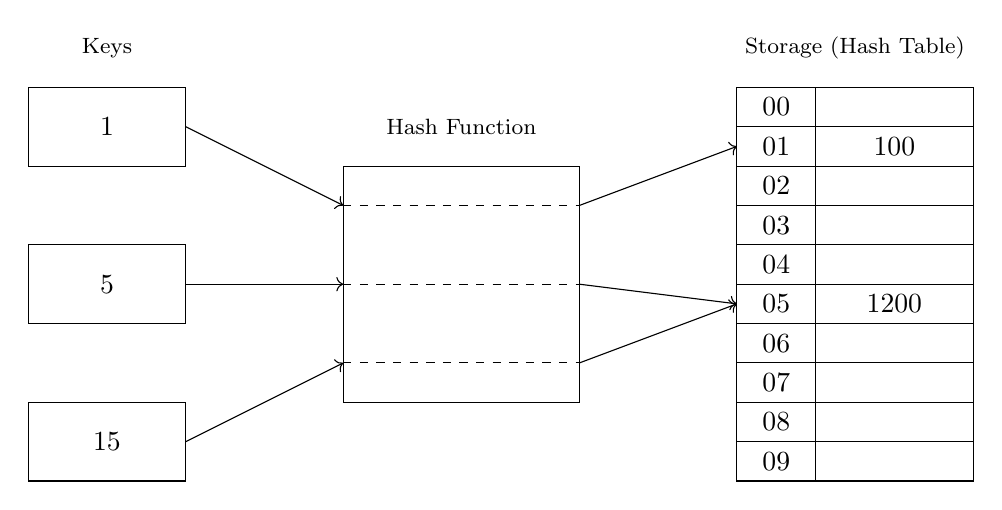
\begin{tikzpicture}
			% Draw the hash function box
			\node at (6.5,4.5) {{\footnotesize Hash Function}};
			\draw (5,1) rectangle (8,4) node[midway] {};
			
			% Draw keys
			\node at (2,5.5) {{\footnotesize Keys}};
			\draw (1,4) rectangle (3,5) node[midway] {1};
			\draw (1,2) rectangle (3,3) node[midway] {5};
			\draw (1,0) rectangle (3,1) node[midway] {15};
			
			% Draw arrows from keys to hash function
			\draw[->] (3,4.5) -- (5,3.5);
			\draw[->] (3,2.5) -- (5,2.5);
			\draw[->] (3,0.5) -- (5,1.5);
			
			\draw[dashed] (5,3.5) -- (8,3.5);
			\draw[dashed] (5,2.5) -- (8,2.5);
			\draw[dashed] (5,1.5) -- (8,1.5);
			
			% Draw the table on the right for values
			\node at (11.5,5.5) {{\footnotesize Storage (Hash Table)}};
			\draw (11,4.5) rectangle (13,5.0) node[midway] {};
			\draw (11,4.0) rectangle (13,4.5) node[midway] {100};
			\draw (11,3.5) rectangle (13,4.0) node[midway] {};
			\draw (11,3.0) rectangle (13,3.5) node[midway] {};
			\draw (11,2.5) rectangle (13,3.0) node[midway] {};
			\draw (11,2.0) rectangle (13,2.5) node[midway] {1200};
			\draw (11,1.5) rectangle (13,2.0) node[midway] {};
			\draw (11,1.0) rectangle (13,1.5) node[midway] {};
			\draw (11,0.5) rectangle (13,1.0) node[midway] {};
			\draw (11,0.0) rectangle (13,0.5) node[midway] {};
			
			\draw (10,4.5) rectangle (11,5.0) node[midway] {00};
			\draw (10,4.0) rectangle (11,4.5) node[midway] {01};
			\draw (10,3.5) rectangle (11,4.0) node[midway] {02};
			\draw (10,3.0) rectangle (11,3.5) node[midway] {03};
			\draw (10,2.5) rectangle (11,3.0) node[midway] {04};
			\draw (10,2.0) rectangle (11,2.5) node[midway] {05};
			\draw (10,1.5) rectangle (11,2.0) node[midway] {06};
			\draw (10,1.0) rectangle (11,1.5) node[midway] {07};
			\draw (10,0.5) rectangle (11,1.0) node[midway] {08};
			\draw (10,0.0) rectangle (11,0.5) node[midway] {09};
			
			% Arrows from hash function to values
			\draw[->] (8,3.5) -- (10,4.25);
			\draw[->] (8,2.5) -- (10,2.25);
			\draw[->] (8,1.5) -- (10,2.25);
			
		\end{tikzpicture}
		\caption{{\footnotesize Visualization of Hash Function and Storage in Hash Table with Collision (200 was replaced by 1200)}}
		\label{fig:hash_table_diagram}
	\end{figure}
	
	We can program the above hash table as:
	
	\begin{lstlisting}[basicstyle=\small]
		#include <stdio.h>
		#include <stdlib.h>
		
		#define TABLE_SIZE 10
		
		typedef struct {
			int key;
			int value;
		} HashEntry;
		
		HashEntry* hashTable[TABLE_SIZE];
		
		// Simple hash function
		int hashFunction(int key) {
			return key % TABLE_SIZE;
		}
		
		void insert(int key, int value) {
			int index = hashFunction(key);
			HashEntry *entry = (HashEntry*)malloc(sizeof(HashEntry));
			entry->key = key;
			entry->value = value;
			hashTable[index] = entry;
		}
		
		int search(int key) {
			int index = hashFunction(key);
			if (hashTable[index] != NULL && hashTable[index]->key == key) {
				return hashTable[index]->value;
			}
			return -1;  // Key not found
		}
		
		int main() {
			insert(1, 100);
			insert(5, 200);
			insert(15, 1200);  // Collision would occur here without handling
			
			printf("Value for key 1: %d\n", search(1));
			printf("Value for key 2: %d\n", search(2));
			printf("Value for key 15: %d\n", search(15));
			
			return 0;
		}
	\end{lstlisting}
	
	The output for the above code is:
	
	\begin{mdframed}[style=myboxstyleTerminal1]
		\begin{verbatim}
			Value for key 1: 100
			Value for key 2: -1
			Value for key 15: 1200
		\end{verbatim}
	\end{mdframed}
	
	
	Run the above code with \codebox{valgrind} to check for memory leak. You will see the following message in the terminal showing the memory leak. 
	
	
	\begin{mdframed}[style=myboxstyleTerminal1]
		\begin{verbatim}
			==35091== HEAP SUMMARY:
			==35091==     in use at exit: 24 bytes in 3 blocks
			==35091==   total heap usage: 4 allocs, 1 frees, 1,048 bytes allocated
			==35091== 
			==35091== 8 bytes in 1 blocks are definitely lost in loss record 3 of 3
			<few more lines here>
			==35091== LEAK SUMMARY:
			==35091==    definitely lost: 8 bytes in 1 blocks
			==35091==    indirectly lost: 0 bytes in 0 blocks
			==35091==      possibly lost: 0 bytes in 0 blocks
			==35091==    still reachable: 16 bytes in 2 blocks
			==35091==         suppressed: 0 bytes in 0 blocks
			==35091== Reachable blocks (those to which a pointer was found) are not shown.
			==35091== To see them, rerun with: --leak-check=full --show-leak-kinds=all
			==35091== 
			==35091== For lists of detected and suppressed errors, rerun with: -s
			==35091== ERROR SUMMARY: 1 errors from 1 contexts (suppressed: 0 from 0)
		\end{verbatim}
	\end{mdframed}
	
	
	I have an array of pointer called \codebox{hashTable}, a global variable, with the size of \codebox{TABLE\_SIZE}. Then each pointer in this array, \codebox{hashTable[i]}, is/will point at a data structure we defined called \codebox{HashEntry}. Three times \codebox{malloc} was used to allocate memory for three \codebox{HashEntry}s, each time \codebox{sizeof(HashEntry)} bytes of memory. In this example, each \codebox{sizeof(HashEntry)} is equal to 8 bytes. \textbf{Why?} The memory allocated by \codebox{insert(5, 200)} is \textbf{definitely lost} since there is no pointer pointing to its address anymore. The pointer \codebox{hashTable[5]} was changed to point at \codebox{HashEntry} with data \codebox{15}. But for the other two memory allocations including \codebox{insert(1, 100)} and \codebox{insert(15, 100)}, the pointers \codebox{hashTable[1]} and \codebox{hashTable[5]} are still pointing at heap addresses holding these two \codebox{HashEntry}s. It is \textbf{still reachable} because the array of pointers \codebox{hashTable} was a global variable and it was not on stack or heap part of memory. \textbf{So where is it?}
	
	In the above example even if we de-allocate the memory for all \codebox{HashEntry}s pointed by \codebox{hashTable[i]}s, still the address to allocated memory for \codebox{insert(5, 200)} is \textbf{definitely lost} and cannot be de-allocated (we don't know where it is or in another word we don't have the address).
	
	
	In real-world scenarios, hash collisions are common, so we need to handle them first. One common technique is \textbf{separate chaining}, where each array index contains a linked list of entries that hash to the same index (Figure \ref{fig:collision}).
	
	\begin{figure}[h!]
		\centering
		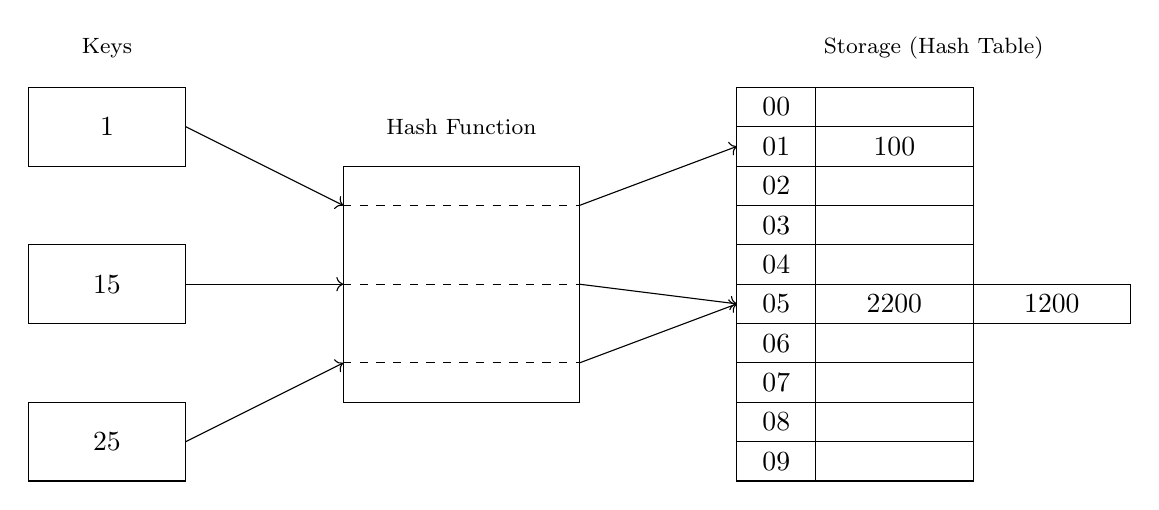
\begin{tikzpicture}
			% Draw the hash function box
			\node at (6.5,4.5) {{\footnotesize Hash Function}};
			\draw (5,1) rectangle (8,4) node[midway] {};
			
			% Draw keys
			\node at (2,5.5) {{\footnotesize Keys}};
			\draw (1,4) rectangle (3,5) node[midway] {1};
			\draw (1,2) rectangle (3,3) node[midway] {15};
			\draw (1,0) rectangle (3,1) node[midway] {25};
			
			% Draw arrows from keys to hash function
			\draw[->] (3,4.5) -- (5,3.5);
			\draw[->] (3,2.5) -- (5,2.5);
			\draw[->] (3,0.5) -- (5,1.5);
			
			\draw[dashed] (5,3.5) -- (8,3.5);
			\draw[dashed] (5,2.5) -- (8,2.5);
			\draw[dashed] (5,1.5) -- (8,1.5);
			
			% Draw the table on the right for values
			\node at (12.5,5.5) {{\footnotesize Storage (Hash Table)}};
			\draw (11,4.5) rectangle (13,5.0) node[midway] {};
			\draw (11,4.0) rectangle (13,4.5) node[midway] {100};
			\draw (11,3.5) rectangle (13,4.0) node[midway] {};
			\draw (11,3.0) rectangle (13,3.5) node[midway] {};
			\draw (11,2.5) rectangle (13,3.0) node[midway] {};
			\draw (11,2.0) rectangle (13,2.5) node[midway] {2200};
			\draw (13,2.0) rectangle (15,2.5) node[midway] {1200};
			\draw (11,1.5) rectangle (13,2.0) node[midway] {};
			\draw (11,1.0) rectangle (13,1.5) node[midway] {};
			\draw (11,0.5) rectangle (13,1.0) node[midway] {};
			\draw (11,0.0) rectangle (13,0.5) node[midway] {};
			
			\draw (10,4.5) rectangle (11,5.0) node[midway] {00};
			\draw (10,4.0) rectangle (11,4.5) node[midway] {01};
			\draw (10,3.5) rectangle (11,4.0) node[midway] {02};
			\draw (10,3.0) rectangle (11,3.5) node[midway] {03};
			\draw (10,2.5) rectangle (11,3.0) node[midway] {04};
			\draw (10,2.0) rectangle (11,2.5) node[midway] {05};
			\draw (10,1.5) rectangle (11,2.0) node[midway] {06};
			\draw (10,1.0) rectangle (11,1.5) node[midway] {07};
			\draw (10,0.5) rectangle (11,1.0) node[midway] {08};
			\draw (10,0.0) rectangle (11,0.5) node[midway] {09};
			
			% Arrows from hash function to values
			\draw[->] (8,3.5) -- (10,4.25);
			\draw[->] (8,2.5) -- (10,2.25);
			\draw[->] (8,1.5) -- (10,2.25);
			
		\end{tikzpicture}
		\caption{{\footnotesize Handling Collision Using Linked Lists}}
		\label{fig:collision}
	\end{figure}
	
	We can program the above procedure as:
	
	\begin{lstlisting}[basicstyle=\small]
		#include <stdio.h>
		#include <stdlib.h>
		
		#define TABLE_SIZE 10
		
		typedef struct HashEntry {
			int key;
			int value;
			struct HashEntry* next;
		} HashEntry;
		
		HashEntry* hashTable[TABLE_SIZE];
		
		// Simple hash function
		int hashFunction(int key) {
			return key % TABLE_SIZE;
		}
		
		void insert(int key, int value) {
			int index = hashFunction(key);
			HashEntry *newEntry = (HashEntry*)malloc(sizeof(HashEntry));
			newEntry->key = key;
			newEntry->value = value;
			newEntry->next = NULL;
			
			// Insert at the beginning of the list for simplicity
			if (hashTable[index] == NULL) {
				hashTable[index] = newEntry;
			} else {
				newEntry->next = hashTable[index];
				hashTable[index] = newEntry;
			}
		}
		
		int search(int key) {
			int index = hashFunction(key);
			HashEntry* entry = hashTable[index];
			while (entry != NULL) {
				if (entry->key == key) {
					return entry->value;
				}
				entry = entry->next;
			}
			return -1;  // Key not found
		}
		
		int main() {
			insert(1, 100);
			insert(15, 1200);  // Collision
			insert(25, 2200);  // Collision
			
			printf("Value for key 15: %d\n", search(15));
			printf("Value for key 25: %d\n", search(25));
			
			return 0;
		}
	\end{lstlisting}
	
	In this example, keys \codebox{15} and \codebox{25} hash to the same index, but collisions are handled by maintaining a linked list at that index. Using \codebox{valgrind} we have:
	
	\begin{mdframed}[style=myboxstyleTerminal1]
		\begin{verbatim}
			==36907== HEAP SUMMARY:
			==36907==     in use at exit: 48 bytes in 3 blocks
			==36907==   total heap usage: 4 allocs, 1 frees, 1,072 bytes allocated
			==36907== 
			==36907== LEAK SUMMARY:
			==36907==    definitely lost: 0 bytes in 0 blocks
			==36907==    indirectly lost: 0 bytes in 0 blocks
			==36907==      possibly lost: 0 bytes in 0 blocks
			==36907==    still reachable: 48 bytes in 3 blocks
			==36907==         suppressed: 0 bytes in 0 blocks
			==36907== Reachable blocks (those to which a pointer was found) are not shown.
			==36907== To see them, rerun with: --leak-check=full --show-leak-kinds=all
			==36907== 
		\end{verbatim}
	\end{mdframed}
	
	It is still a garbage code. It has memory leak. But it is much better! Each pointer \codebox{hashTable[i]} is pointing at a \codebox{HashEntry}. Simply I can de-allocate \codebox{sizeof(HashEntry)}\textbf{s}, using \textbf{their} pointers \codebox{free(hashTable[i])}\textbf{s}. Update the code into the following format:
	
	\begin{lstlisting}
		
		// <the same as previous verison with hash collision handling>
		
		void freeHashTable(){
			for (int i = 0; i < TABLE_SIZE; i++){
				free(hashTable[i]);
			}
		}
		
		int main(){
			
			insert(1, 100);
			insert(15, 1200); // Collision
			insert(25, 2200); // Collision
			
			freeHashTable();
			
			return 0;
		}
	\end{lstlisting}
	
	
	Running the code with \codebox{valgrind} is giving us:
	
	\begin{mdframed}[style=myboxstyleTerminal1]
		\begin{verbatim}
			==37615== HEAP SUMMARY:
			==37615==     in use at exit: 16 bytes in 1 blocks
			==37615==   total heap usage: 4 allocs, 3 frees, 1,072 bytes allocated
			==37615== 
			==37615== 16 bytes in 1 blocks are definitely lost in loss record 1 of 1
			<few more lines>
			==37615== LEAK SUMMARY:
			==37615==    definitely lost: 16 bytes in 1 blocks
			==37615==    indirectly lost: 0 bytes in 0 blocks
			==37615==      possibly lost: 0 bytes in 0 blocks
			==37615==    still reachable: 0 bytes in 0 blocks
			==37615==         suppressed: 0 bytes in 0 blocks
			==37615== 
			==37615== For lists of detected and suppressed errors, rerun with: -s
			==37615== ERROR SUMMARY: 1 errors from 1 contexts (suppressed: 0 from 0)
		\end{verbatim}
	\end{mdframed}
	
	Still we have memory leak! By freeing the memory with the above format, only the first \codebox{HashEntry} that \codebox{hashTable[5]} is pointing at is being de-allocated. This means the memory allocated \codebox{insert(15, 1200);} is left behind. Change the \codebox{freeHashTable()} to the following format to handle collision while de-allocating the memory.
	
	\begin{lstlisting}
		void freeHashTable(){
			for (int i = 0; i < TABLE_SIZE; i++){
				HashEntry *temp = hashTable[i];
				while (temp){// temp!=NULL
					HashEntry *toFree = temp;
					temp = temp->next;
					free(toFree);
				}
			}
		}
	\end{lstlisting}
	
	Run the code with \codebox{valgrind} and this time you should see:
	
	\begin{mdframed}[style=myboxstyleTerminal1]
		\begin{verbatim}
			==38235== HEAP SUMMARY:
			==38235==     in use at exit: 0 bytes in 0 blocks
			==38235==   total heap usage: 4 allocs, 4 frees, 1,072 bytes allocated
			==38235== 
			==38235== All heap blocks were freed -- no leaks are possible
			==38235== 
			==38235== For lists of detected and suppressed errors, rerun with: -s
			==38235== ERROR SUMMARY: 0 errors from 0 contexts (suppressed: 0 from 0)
		\end{verbatim}
	\end{mdframed}
	
	Well Done! Now there is only one more thing I don't like about the above code. Why the memory for pointer or the array of pointers \codebox{hashTable} is global variable instead of being allocated on heap? Changing that can create minor changes in your code format:
	
	\begin{lstlisting}
		#include <stdio.h>
		#include <stdlib.h>
		
		#define TABLE_SIZE 10
		
		typedef struct HashEntry{
			int key;   // SN
			int value; // FN or LS etc
			struct HashEntry *next;
		} HashEntry;
		
		// Simple hash function
		int hashFunction(int key){ // keys: 1, 5, 15,
			return key % TABLE_SIZE; // index: 1, 5, 5
		}
		
		void insert(HashEntry **hashTable, int key, int value){
			int index = hashFunction(key);
			HashEntry *entry = (HashEntry *)malloc(sizeof(HashEntry));
			entry->key = key;
			entry->value = value;
			entry->next = hashTable[index];
			hashTable[index] = entry;
		}
		
		int search(HashEntry **hashTable, int key){
			int index = hashFunction(key);
			HashEntry *current = hashTable[index];
			while (current != NULL)
			{
				if (current->key == key)
				{
					return current->value;
				}
				current = current->next;
			}
			return -1; // -1 as value
		}
		
		void printHashTable(HashEntry **hashTable){
			for (int i = 0; i < TABLE_SIZE; i++){
				HashEntry *current = hashTable[i];
				printf("hashTable[%d] -> ", i);
				while (current){
					printf("%d -> ", current->value);
					current = current->next;
				}
				printf("NULL\n");
			}
		}
		
		void freeHashTable(HashEntry **hashTable){
			
			for (int i = 0; i < TABLE_SIZE; i++){
				HashEntry *temp = hashTable[i];
				while (temp){ // temp!=NULL
					HashEntry *toFree = temp;
					temp = temp->next;
					free(toFree);
				}
			}
			free(hashTable);
		}
		
		int main(){
			// HashEntry *hashTable[TABLE_SIZE];
			// memory alloc
			HashEntry **hashTable = (HashEntry **)calloc(TABLE_SIZE, sizeof(HashEntry *));
			
			insert(hashTable, 1, 100);
			insert(hashTable, 5, 200);
			insert(hashTable, 15, 1200); // Collision would occur here without handling
			
			printf("Value for key 1: %d\n", search(hashTable, 1));
			printf("Value for key 5: %d\n", search(hashTable, 5));
			printf("Value for key 15: %d\n\n", search(hashTable, 15));
			
			printHashTable(hashTable);
			
			freeHashTable(hashTable);
			
			return 0;
		}
	\end{lstlisting}
	
	The above code should output:
	
	\begin{mdframed}[style=myboxstyleTerminal1]
		\begin{verbatim}
			Value for key 1: 100
			Value for key 5: 200
			Value for key 15: 1200
			
			hashTable[0] -> NULL
			hashTable[1] -> 100 -> NULL
			hashTable[2] -> NULL
			hashTable[3] -> NULL
			hashTable[4] -> NULL
			hashTable[5] -> 1200 -> 200 -> NULL
			hashTable[6] -> NULL
			hashTable[7] -> NULL
			hashTable[8] -> NULL
			hashTable[9] -> NULL
		\end{verbatim}
	\end{mdframed}
	
	
	Hashing is often used with string keys (Figure \ref{fig:hash_table_string}), especially in dictionary-like structures. A more advanced example is using strings as keys in a hash map. We need a \textbf{string hashing function} like the \textbf{djb2} hash function.
	
	\begin{figure}[h!]
		\centering
		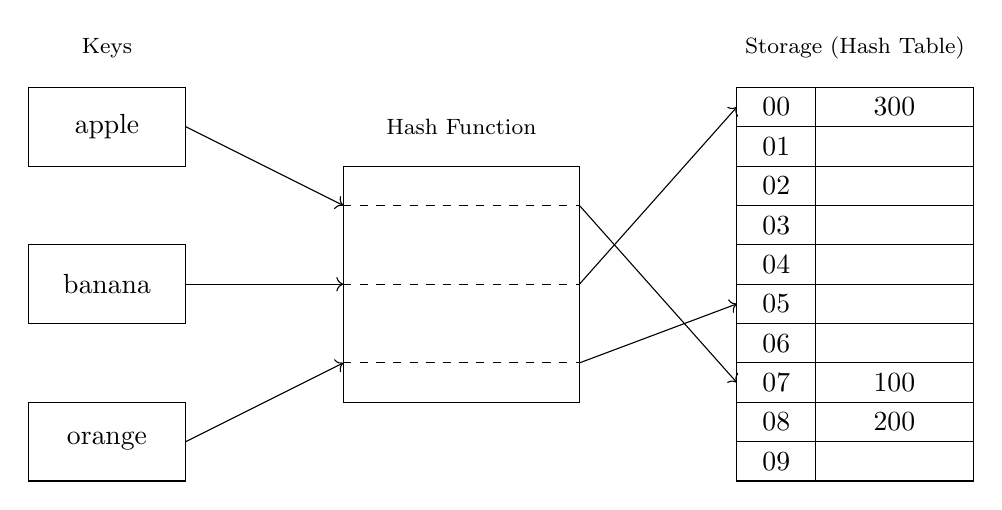
\begin{tikzpicture}
			% Draw the hash function box
			\node at (6.5,4.5) {{\footnotesize Hash Function}};
			\draw (5,1) rectangle (8,4) node[midway] {};
			
			% Draw keys
			\node at (2,5.5) {{\footnotesize Keys}};
			\draw (1,4) rectangle (3,5) node[midway] {apple};
			\draw (1,2) rectangle (3,3) node[midway] {banana};
			\draw (1,0) rectangle (3,1) node[midway] {orange};
			
			% Draw arrows from keys to hash function
			\draw[->] (3,4.5) -- (5,3.5);
			\draw[->] (3,2.5) -- (5,2.5);
			\draw[->] (3,0.5) -- (5,1.5);
			
			\draw[dashed] (5,3.5) -- (8,3.5);
			\draw[dashed] (5,2.5) -- (8,2.5);
			\draw[dashed] (5,1.5) -- (8,1.5);
			
			% Draw the table on the right for values
			\node at (11.5,5.5) {{\footnotesize Storage (Hash Table)}};
			\draw (11,4.5) rectangle (13,5.0) node[midway] {300};
			\draw (11,4.0) rectangle (13,4.5) node[midway] {};
			\draw (11,3.5) rectangle (13,4.0) node[midway] {};
			\draw (11,3.0) rectangle (13,3.5) node[midway] {};
			\draw (11,2.5) rectangle (13,3.0) node[midway] {};
			\draw (11,2.0) rectangle (13,2.5) node[midway] {};
			\draw (11,1.5) rectangle (13,2.0) node[midway] {};
			\draw (11,1.0) rectangle (13,1.5) node[midway] {100};
			\draw (11,0.5) rectangle (13,1.0) node[midway] {200};
			\draw (11,0.0) rectangle (13,0.5) node[midway] {};
			
			\draw (10,4.5) rectangle (11,5.0) node[midway] {00};
			\draw (10,4.0) rectangle (11,4.5) node[midway] {01};
			\draw (10,3.5) rectangle (11,4.0) node[midway] {02};
			\draw (10,3.0) rectangle (11,3.5) node[midway] {03};
			\draw (10,2.5) rectangle (11,3.0) node[midway] {04};
			\draw (10,2.0) rectangle (11,2.5) node[midway] {05};
			\draw (10,1.5) rectangle (11,2.0) node[midway] {06};
			\draw (10,1.0) rectangle (11,1.5) node[midway] {07};
			\draw (10,0.5) rectangle (11,1.0) node[midway] {08};
			\draw (10,0.0) rectangle (11,0.5) node[midway] {09};
			
			% Arrows from hash function to values
			\draw[->] (8,3.5) -- (10,1.25);
			\draw[->] (8,2.5) -- (10,4.75);
			\draw[->] (8,1.5) -- (10,2.25);
			
		\end{tikzpicture}
		\caption{{\footnotesize Hash Function and Storage in Hash Table in Strings}}
		\label{fig:hash_table_string}
	\end{figure}
	
	\begin{lstlisting}[basicstyle=\small]
		#include <stdio.h>
		#include <stdlib.h>
		#include <string.h>
		
		#define TABLE_SIZE 10
		
		typedef struct HashEntry{
			char *key;
			int value;
			struct HashEntry *next;
		} HashEntry;
		
		// Hash function for strings (djb2 algorithm)
		unsigned long hashFunction(char *str){
			unsigned long hash = 5381;
			int c;
			while ((c = *str++)){
				hash = ((hash << 5) + hash) + c; // hash << 5 = hash * 2^5
			}
			return hash % TABLE_SIZE;
		}
		
		void insert(HashEntry **hashTable, char *key, int value){
			unsigned long index = hashFunction(key);
			HashEntry *newEntry = (HashEntry *)malloc(sizeof(HashEntry));
			newEntry->key = strdup(key); // Duplicate string
			newEntry->value = value;
			newEntry->next = hashTable[index]; // collision is handled
			hashTable[index] = newEntry;
		}
		
		int search(HashEntry **hashTable, char *key){
			unsigned long index = hashFunction(key);
			HashEntry *entry = hashTable[index];
			while (entry != NULL){
				if (strcmp(entry->key, key) == 0){
					return entry->value;
				}
				entry = entry->next;
			}
			return -1; // Key not found
		}
		
		void printHashTable(HashEntry **hashTable){
			for (int i = 0; i < TABLE_SIZE; i++){
				HashEntry *current = hashTable[i];
				printf("hashTable[%d] -> ", i);
				while (current){
					printf("(%s, %d, pointer) -> ", current->key, current->value);
					current = current->next;
				}
				printf("NULL\n");
			}
			
		}
		
		void freeMemoryTable(HashEntry **hashTable){
			for (int i = 0; i < TABLE_SIZE; i++){
				HashEntry *current = hashTable[i];
				while (current){
					HashEntry *toFree = current;
					current = current->next;
					free(toFree->key);
					free(toFree);
				}
			}
			free(hashTable);
		}
		
		int main(){
			HashEntry **hashTable = calloc(TABLE_SIZE, sizeof(HashEntry*));
			
			insert(hashTable, "apple", 100);
			insert(hashTable, "banana", 200);
			insert(hashTable, "orange", 300);
			
			printf("Value for 'apple': %d\n", search(hashTable, "apple"));
			printf("Value for 'banana': %d\n", search(hashTable, "banana"));
			printf("Value for 'cherry': %d\n", search(hashTable, "cherry"));
			
			printHashTable(hashTable);
			freeMemoryTable(hashTable);
			
			return 0;
		}
	\end{lstlisting}
	
	In this example, the \textbf{djb2} hash function processes strings, and the hash map stores key-value pairs where the keys are strings. Collisions are handled using linked lists, as before. The above code will output:
	
	\begin{mdframed}[style=myboxstyleTerminal1]
		\begin{verbatim}
			Value for 'apple': 100
			Value for 'banana': 200
			Value for 'cherry': -1
			hashTable[0] -> (banana, 200, pointer) -> NULL
			hashTable[1] -> NULL
			hashTable[2] -> NULL
			hashTable[3] -> NULL
			hashTable[4] -> NULL
			hashTable[5] -> (orange, 300, pointer) -> NULL
			hashTable[6] -> NULL
			hashTable[7] -> (apple, 100, pointer) -> NULL
			hashTable[8] -> NULL
			hashTable[9] -> NULL
		\end{verbatim}
	\end{mdframed}
	
	
	\textbf{Additional Considerations}:
	
	\begin{itemize}
		\item Load Factor: The performance of a hash table is dependent on the load factor, which is the ratio of the number of entries to the table size. High load factors can lead to more collisions and performance degradation.
		
		\item Open Addressing: Another method to resolve collisions is open addressing, where instead of using linked lists, we probe the hash table for the next available slot.
	\end{itemize}
	
	
	
	
	
	
	\section{Linked List}
	
	A Linked List is a linear data structure where elements are stored in nodes. Each node contains two parts:
	
	\begin{enumerate}
		\item \textbf{Data}: The actual value or information stored in the node.
		\item \textbf{Pointer (next)}: A reference (or pointer) to the next node in the list.
	\end{enumerate}
	
	
	Unlike arrays, linked lists are not stored in contiguous memory locations. Instead, each element points to the next, allowing for dynamic memory allocation. This flexibility makes linked lists useful for scenarios where you do not know the size of the dataset in advance or need frequent insertions and deletions.
	
	Linked lists are fundamental in many computer science applications, and they serve as the foundation for more complex data structures like stacks, queues, and graphs.
	
	\textbf{Types} of Linked Lists shown in Figure \ref{fig:intro_linked_lists} are:
	
	\begin{itemize}
		\item Singly Linked List: Each node contains a single pointer pointing to the next node.
		\item Doubly Linked List: Each node contains two pointers, one pointing to the next node and another pointing to the previous node.
		\item Circular Linked List: The last node points back to the first node, forming a circular chain.
	\end{itemize}
	
	
	\begin{figure}[h!]
		\centering
		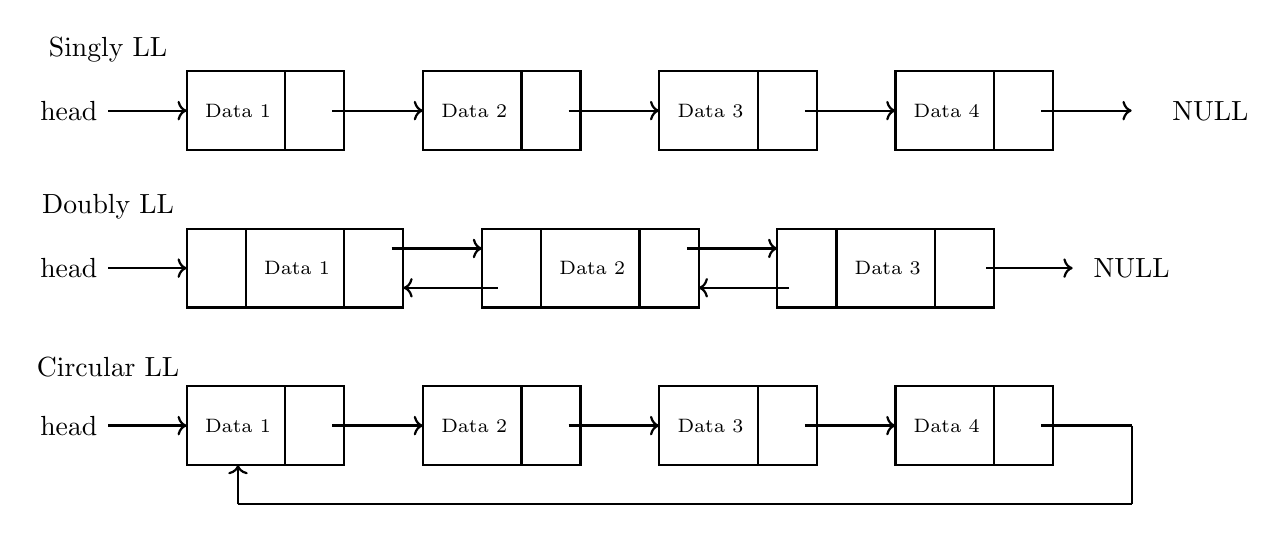
\begin{tikzpicture}
			% Singly Linked List
			\draw[thick] (0,3) rectangle (1.25,4);
			\draw[thick] (1.25,3) rectangle (2,4);
			\node at (0.65,3.5) {{\scriptsize Data 1}};
			\draw[->, thick] (1.85,3.5) -- (3,3.5);
			\draw[thick] (3,3) rectangle (4.25,4);
			\draw[thick] (4.25,3) rectangle (5,4);
			\node at (3.65,3.5) {{\scriptsize Data 2}};
			\draw[->, thick] (4.85,3.5) -- (6,3.5);
			\draw[thick] (6,3) rectangle (7.25,4);
			\draw[thick] (7.25,3) rectangle (8,4);
			\node at (6.65,3.5) {{\scriptsize Data 3}};
			\draw[->, thick] (7.85,3.5) -- (9,3.5);
			\draw[thick] (9,3) rectangle (10.25,4);
			\draw[thick] (10.25,3) rectangle (11,4);
			\node at (9.65,3.5) {{\scriptsize Data 4}};
			\draw[->, thick] (10.85,3.5) -- (12,3.5);
			\node at (13,3.5) {NULL};
			
			% Label for head node
			\node at (-1.5,3.5) {head};
			\node[above] at (-1,4) {Singly LL};
			\draw[->, thick] (-1,3.5) -- (0,3.5);
			
			
			
			% Doubly Linked List
			\draw[thick] (0,1) rectangle (0.75,2);
			\draw[thick] (0.75,1) rectangle (2,2);
			\draw[thick] (2,1) rectangle (2.75,2);
			\node at (1.4,1.5) {{\scriptsize Data 1}};
			\draw[->, thick] (2.6,1.75) -- (3.75,1.75);
			\draw[->, thick] (3.95,1.25) -- (2.75,1.25);
			
			\draw[thick] (3.75,1) rectangle (4.5,2);
			\draw[thick] (4.5,1) rectangle (5.75,2);
			\draw[thick] (5.75,1) rectangle (6.5,2);
			\node at (5.15,1.5) {{\scriptsize Data 2}};
			\draw[->, thick] (6.35,1.75) -- (7.5,1.75);
			\draw[->, thick] (7.65,1.25) -- (6.5,1.25);
			
			\draw[thick] (7.5,1) rectangle (8.25,2);
			\draw[thick] (8.25,1) rectangle (9.5,2);
			\draw[thick] (9.5,1) rectangle (10.25,2);
			\node at (8.9,1.5) {{\scriptsize Data 3}};
			\draw[->, thick] (10.15,1.5) -- (11.25,1.5);
			\node at (12,1.5) {NULL};
			
			
			% Label for head node
			\node at (-1.5,1.5) {head};
			\node[above] at (-1,2) {Doubly LL};
			\draw[->, thick] (-1,1.5) -- (0,1.5);
			
			
			
			% Circular Linked List
			\draw[thick] (0,-1) rectangle (1.25,0);
			\draw[thick] (1.25,-1) rectangle (2,0);
			\node at (0.65,-0.5) {{\scriptsize Data 1}};
			\draw[->, thick] (1.85,-0.5) -- (3,-0.5);
			\draw[thick] (3,-1) rectangle (4.25,0);
			\draw[thick] (4.25,-1) rectangle (5,0);
			\node at (3.65,-0.5) {{\scriptsize Data 2}};
			\draw[->, thick] (4.85,-0.5) -- (6,-0.5);
			\draw[thick] (6,-1) rectangle (7.25,0);
			\draw[thick] (7.25,-1) rectangle (8,0);
			\node at (6.65,-0.5) {{\scriptsize Data 3}};
			\draw[->, thick] (7.85,-0.5) -- (9,-0.5);
			\draw[thick] (9,-1) rectangle (10.25,0);
			\draw[thick] (10.25,-1) rectangle (11,0);
			\node at (9.65,-0.5) {{\scriptsize Data 4}};
			\draw[, thick] (10.85,-0.5) -- (12,-0.5);
			\draw[, thick] (12,-0.5) -- (12,-1.5);
			\draw[, thick] (12,-1.5) -- (0.65,-1.5);
			\draw[->, thick] (0.65,-1.5) -- (0.65,-1);
			
			
			% Label for head node
			\node at (-1.5,-0.5) {head};
			\node[above] at (-1,0) {Circular LL};
			\draw[->, thick] (-1,-0.5) -- (0,-0.5);
			
			
			
			
		\end{tikzpicture}
		\caption{{\footnotesize Linked List (LL) Data Structure}}
		\label{fig:intro_linked_lists}
	\end{figure}
	
	\textbf{Advantages} of Linked Lists:
	
	\begin{itemize}
		\item Dynamic Size: Linked lists can grow and shrink as needed.
		\item Efficient Insertions/Deletions: Inserting or deleting an element at any position (especially in the middle) is faster compared to arrays, as no shifting is required.
	\end{itemize}
	
	
	
	\textbf{Disadvantages} of Linked Lists:
	
	\begin{itemize}
		\item Random Access: Linked lists don’t allow random access. To access a node, you must traverse the list from the beginning.
		\item Memory Overhead: Each node requires extra memory for the pointer to the next node.
	\end{itemize}
	
	Here is a basic example of \textbf{Singly} Linked List Implementation in C:
	
	\begin{lstlisting}
		#include <stdio.h>
		#include <stdlib.h>
		
		// Node structure
		typedef struct Node {
			int data;
			struct Node* next;
		}Node;
		
		// Function to create a new node
		Node* createNode(int data) {
			struct Node* newNode = (Node*)malloc(sizeof(Node));
			newNode->data = data;
			newNode->next = NULL;
			return newNode;
		}
		
		// Function to print the linked list
		void printList(Node* head) {
			Node* temp = head;
			while (temp != NULL) {
				printf("%d -> ", temp->data);
				temp = temp->next;
			}
			printf("NULL\n");
		}
		
		// Function to insert a new node at the end
		void appendNode(Node** head, int data) {
			Node* newNode = createNode(data);
			if (*head == NULL) {
				*head = newNode;
				return;
			}
			Node* temp = *head;
			while (temp->next != NULL) {
				temp = temp->next;
			}
			temp->next = newNode;
		}
		
		void FreeList(Node *head){
			Node *temp;
			while (head){
				temp = head;
				head = head->next;
				free(temp);
			}
		}
		
		// Main function
		int main() {
			Node* head = NULL;
			
			// Inserting nodes
			appendNode(&head, 10);
			appendNode(&head, 20);
			appendNode(&head, 30);
			
			// Printing the list
			printList(head);
			FreeList(head);
			return 0;
		}
	\end{lstlisting}
	
	This code defines a singly linked list. It demonstrates how to create a new node and append it to the end of the list. The \codebox{printList} function traverses the list from the head to the last node:
	
	\begin{mdframed}[style=myboxstyleTerminal1]
		\begin{verbatim}
			10 -> 20 -> 30 -> NULL
		\end{verbatim}
	\end{mdframed}
	
	Sometimes it is necessary to insert a \codebox{Node} at the beginning of list:
	
	\begin{lstlisting}
		void insertAtBeginning(Node** head, int data) {
			Node* newNode = createNode(data);
			newNode->next = *head;
			*head = newNode;
		}
	\end{lstlisting}
	
	Here, the new node is inserted at the beginning of the list. The new node's next pointer points to the current head, and the head is updated to the new node.
	
	\textbf{Reversing} a singly linked list is a common operation where you reverse the direction of the pointers in the list:
	
	\begin{lstlisting}
		Node* reverseList(Node* head) {
			Node* prev = NULL;
			Node* current = head;
			Node* next = NULL;
			
			while (current != NULL) {
				next = current->next;   // Store the next node
				current->next = prev;   // Reverse the current node's pointer
				prev = current;         // Move pointers one position ahead
				current = next;
			}
			return prev;
		}
	\end{lstlisting}
	
	The above function has a time Complexity of $O(n)$, where n is the number of nodes, and a space complexity of $O(1)$, since we only use a few extra pointers. You can add the following code into the \codebox{main()} to test your function:
	
	\begin{lstlisting}
		Node* ReversedHead = reverseList(head);
		printList(ReversedHead);
	\end{lstlisting}
	
	This will give you:
	
	\begin{mdframed}[style=myboxstyleTerminal1]
		\begin{verbatim}
			30 -> 20 -> 10 -> NULL
		\end{verbatim}
	\end{mdframed}
	
	After reversing \codebox{head} and returning \codebox{ReversedHead}, \textbf{how should we de-allocate the memory?} Should we de-allocate the memory one time for \codebox{head} and another time for \codebox{ReversedHead}?
	
	\textbf{Merging} two sorted linked lists into one sorted list is another common problem:
	
	\begin{lstlisting}
		Node* mergeSortedLists(Node* l1, Node* l2) {
			if (!l1) return l2;
			if (!l2) return l1;
			
			if (l1->data < l2->data) {
				l1->next = mergeSortedLists(l1->next, l2);
				return l1;
			} else {
				l2->next = mergeSortedLists(l1, l2->next);
				return l2;
			}
		}
	\end{lstlisting}
	
	The function recursively merges two sorted lists. If \codebox{l1}'s data is smaller, the function moves to the next node in \codebox{l1}, otherwise, it moves to the next node in \codebox{l2}. You can test the above function by creating two lists, let's say \codebox{head1} and \codebox{head2}, pass two lists to function, and saved the returned linked list into another list, say \codebox{MergedList}, then print the results with \codebox{printList}. Should we de-allocate the memory for initial two lists and return merged list separately?
	
	Another commonly used operation on linked list is \textbf{removing} Nth node from end of list: 
	
	\begin{lstlisting}
		Node* removeNthFromEnd(Node* head, int n) {
			Node* dummy = createNode(0);
			dummy->next = head;
			Node *first = dummy, *second = dummy;
			
			for (int i = 0; i <= n; i++) {
				first = first->next;
			}
			
			while (first != NULL) {
				first = first->next;
				second = second->next;
			}
			
			Node* toDelete = second->next;
			second->next = second->next->next;
			free(toDelete);
			
			return dummy->next;
		}
	\end{lstlisting}
	
	This algorithm uses two pointers. The first pointer is moved n nodes ahead. Then both pointers move together until the first pointer reaches the end. This way, the second pointer ends up at the node right before the node to be removed. Test the above function by adding the following code into \codebox{main()}:
	
	\begin{lstlisting}
		Node* RemovedNth = removeNthFromEnd(head,1);
		printList(RemovedNth);
	\end{lstlisting}
	
	This will give you:
	
	
	\begin{mdframed}[style=myboxstyleTerminal1]
		\begin{verbatim}
			10 -> 20 -> NULL
		\end{verbatim}
	\end{mdframed}
	
	\textbf{Why is \codebox{head} or initial lists are changed even though we returned a new pointer in all above functions?} Probably you have noticed after calling a function like \codebox{removeNthFromEnd()} the original \codebox{head} list is changed (the same as \codebox{RemovedNth}). This happens because C passes pointers by value, meaning the function receives a copy of the pointer \codebox{head}, but the copy still points to the same memory as the original. Any changes made to the list via this pointer will affect the original list, including when nodes are removed or restructured.
	
	Linked lists are a fundamental data structure that offer great flexibility in managing dynamically sized data. Their ability to efficiently insert and delete elements, combined with their simplicity, makes them essential in many real-world applications. Mastering the different operations on linked lists (insertion, deletion, traversal, and searching) is crucial for understanding more complex data structures and algorithms. Obviously, there is not enough time to cover all those function in this course. Please feel free to reach out if you are looking for some online resource to practice. Meanwhile you can start with the following exercises:
	
	\begin{itemize}
		\item Implement a function that removes duplicates from a sorted linked list.
		\item Implement a function that checks if a linked list has a cycle.
	\end{itemize}
	
	These tasks build the foundational skills necessary to move on to more advanced data structures like doubly linked lists and circular linked lists.
	
	
	
	
	
	
	
	
	
	
	
	
	
	\section{Stack}
	
	
	A stack is a linear data structure that follows the \textbf{Last In}, \textbf{First Out} (\textbf{LIFO}) principle, meaning the last element added to the stack is the first one to be removed. Think of a stack like a pile of books: you can only remove or add a book to the top of the stack. This structure is widely used in computer science for tasks like function call management, expression evaluation, undo mechanisms in text editors, depth-first search in graphs, and more.
	
	Key operations in a stack (Figure \ref{fig:intro_stack}) are:
	
	\begin{itemize}
		\item \textbf{Push}: Adds an element to the top of the stack.
		\item \textbf{Pop}: Removes the element from the top of the stack.
		\item \textbf{Peek/Top}: Returns the top element without removing it.
		\item \textbf{isEmpty}: Checks if the stack is empty.
	\end{itemize}
	
	\begin{figure}[h!]
		\centering
		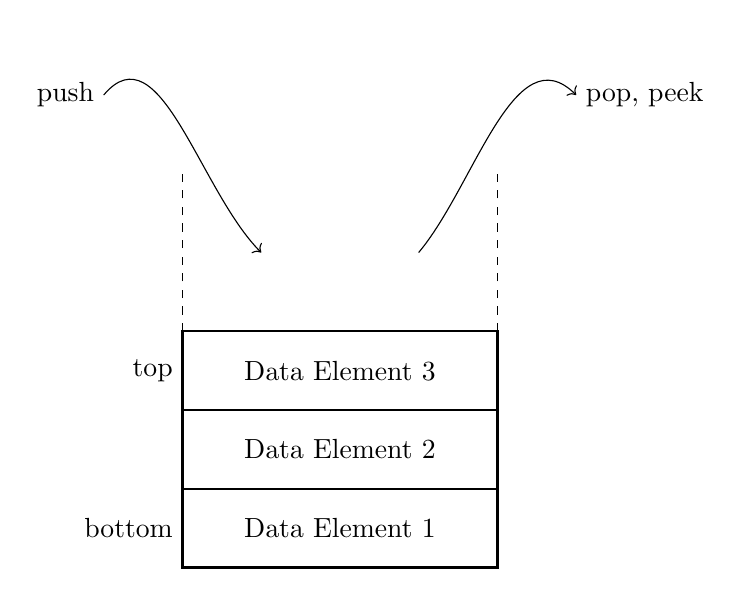
\begin{tikzpicture}
			% Stack rectangle
			\draw[thick] (-1,0) rectangle (3,3);
			
			% Dividing lines for stack elements
			\draw[thick] (-1,1) -- (3,1);
			\draw[thick] (-1,2) -- (3,2);
			
			\draw[dashed] (3,3) -- (3,5);
			\draw[dashed] (-1,3) -- (-1,5);
			
			% Stack elements text
			\node at (1,2.5) {Data Element 3};
			\node at (1,1.5) {Data Element 2};
			\node at (1,0.5) {Data Element 1};
			
			% Labels for top and bottom
			\node[left] at (-1,2.5) {top};
			\node[left] at (-1,0.5) {bottom};
			
			% Arrow for push
			\draw[->] (-2,6) node[left] {push} to[out=+50] (0,4);
			
			% Arrow for pop and peek
			\draw[->] (2,4)  to[out=+50] (4,6) node[right] {pop, peek};
		\end{tikzpicture}
		\caption{{\footnotesize Stack Data Structure}}
		\label{fig:intro_stack}
	\end{figure}
	
	
	Stacks are used in:
	
	\begin{itemize}
		\item Expression Evaluation: Converting and evaluating expressions like infix, postfix, or prefix.
		\item Recursion: Function calls are managed using a call stack.
		\item Undo Mechanisms: Maintaining a history of operations in applications like text editors.
		\item Backtracking Algorithms: Such as depth-first search (DFS) in graph traversal.
		\item Memory Management: Keeping track of memory during function calls (stack memory).
	\end{itemize}
	
	
	A stack can be implemented in two ways:
	
	\begin{enumerate}
		\item Array-based Implementation (Fixed size)
		\item Linked List-based Implementation (Dynamic size)
	\end{enumerate}
	
	We'll start with a basic array-based implementation and gradually move to more advanced topics. Here’s a simple example of how to implement a \textbf{stack using arrays} in C:
	
	\begin{lstlisting}
		#include <stdio.h>
		#include <stdlib.h>
		
		#define MAX 5  // Define maximum size for the stack
		
		typedef struct Stack {
			int arr[MAX];
			int top;
		}Stack;
		
		// Initialize stack
		void initStack(Stack *stack) {
			stack->top = -1;
		}
		
		// Check if stack is full
		int isFull(Stack *stack) {
			return stack->top == MAX - 1;
		}
		
		// Check if stack is empty
		int isEmpty(Stack *stack) {
			return stack->top == -1;
		}
		
		// Push an element onto the stack
		void push(Stack *stack, int value) {
			if (isFull(stack)) {
				printf("Stack Overflow\n");
				return;
			}
			stack->arr[++stack->top] = value;
			printf("Pushed %d onto the stack\n", value);
		}
		
		// Pop an element from the stack
		int pop(Stack *stack) {
			if (isEmpty(stack)) {
				printf("Stack Underflow\n");
				return -1;
			}
			return stack->arr[stack->top--];
		}
		
		// Peek at the top element
		int peek(Stack *stack) {
			if (isEmpty(stack)) {
				printf("Stack is empty\n");
				return -1;
			}
			return stack->arr[stack->top];
		}
		
		int main() {
			Stack stack;
			initStack(&stack);
			
			push(&stack, 10);
			push(&stack, 20);
			push(&stack, 30);
			
			printf("Top element is %d\n", peek(&stack));
			
			printf("Popped element is %d\n", pop(&stack));
			printf("Popped element is %d\n", pop(&stack));
			
			return 0;
		}
	\end{lstlisting}
	
	In this basic implementation:
	
	\begin{itemize}
		\item We define a stack with a maximum size using an array.
		\item The stack operations (push, pop, peek, isFull, isEmpty) are defined as functions that modify the stack.
		\item Overflow and underflow conditions are handled, ensuring that we can't add more elements than the defined maximum, and we can't remove elements from an empty stack.
	\end{itemize}
	
	
	A \textbf{linked list-based implementation of a stack} provides flexibility as it allows dynamic size. Each node in the stack is dynamically allocated memory, and we can easily push or pop elements without worrying about the predefined size limit.
	
	\begin{lstlisting}
		#include <stdio.h>
		#include <stdlib.h>
		
		typedef struct Node{
			int data;
			struct Node *next;
		} Node;
		
		// Check if the stack is empty
		int isEmpty(Node *top){
			return top == NULL;
		}
		
		// Push an element onto the stack
		void push(Node **top, int value){
			Node *newNode = (Node *)malloc(sizeof(Node));
			if (!newNode){
				printf("Heap Overflow\n");
				exit(1);
			}
			newNode->data = value;
			newNode->next = *top;
			*top = newNode;
			printf("Pushed %d onto the stack\n", value);
		}
		
		// Pop an element from the stack
		int pop(Node **top){
			if (isEmpty(*top)){
				printf("Stack Underflow\n");
				return -1;
			}
			Node *temp = *top;
			int poppedValue = temp->data;
			*top = (*top)->next;
			free(temp);
			return poppedValue;
		}
		
		// Peek at the top element
		int peek(Node *top){
			if (isEmpty(top)){
				printf("Stack is empty\n");
				return -1;
			}
			return top->data;
		}
		
		void FreeStackList(Node *head){
			Node *temp;
			while (head){
				temp = head;
				head = head->next;
				free(temp);
			}
		}
		
		int main(){
			Node *stack = NULL;
			
			push(&stack, 10);
			push(&stack, 20);
			push(&stack, 30);
			
			printf("Top element is %d\n", peek(stack));
			
			printf("Popped element is %d\n", pop(&stack));
			printf("Popped element is %d\n", pop(&stack));
			
			FreeStackList(stack);
			return 0;
		}
		
	\end{lstlisting}
	
	
	In this implementation:
	
	\begin{itemize}
		\item Each element (node) of the stack contains data and a pointer to the next element.
		\item We can dynamically allocate and deallocate memory as elements are pushed or popped from the stack.
		\item This implementation avoids the fixed size limitation of array-based stacks.
	\end{itemize}
	
	
	Depending on the required flexibility, stacks can have different designs. Let's solve Generate Parentheses problem. Given \codebox{n} pairs of parentheses, write a function to generate all combinations of well-formed parentheses. For example when \codebox{n = 3} then the output is:
	
	\begin{mdframed}[style=myboxstyleTerminal1]
		\begin{verbatim}
			["((()))","(()())","(())()","()(())","()()()"]
		\end{verbatim}
	\end{mdframed}
	
	
	While the example of generating valid parentheses combinations doesn't directly involve an explicit stack data structure in the solution, the underlying concept of managing balanced parentheses does relate to stack-like behavior. Here's why:
	
	\begin{enumerate}
		\item Balanced Parentheses Problem:
		
		\begin{itemize}
			\item The idea of generating or validating balanced parentheses is a classic use case of a stack. When you add an opening parenthesis \codebox{(}, it's like "pushing" it onto a stack, and when you add a closing parenthesis \codebox{)}, you "pop" an opening parenthesis from the stack to match it.
			\item If you were asked to validate whether a given string of parentheses is well-formed, the best approach would be using a stack, where you push \codebox{(} and pop when encountering \codebox{)}. If the stack is empty at the end, the string is valid.
		\end{itemize}
		
		\item Implicit Stack in Recursion:
		
		\begin{itemize}
			\item Recursion itself uses the call stack, where each recursive call pushes the current state onto the stack and returns (or pops) when done. In this sense, the recursive function in your solution is behaving similarly to a stack.
			\item Each recursive call in your solution corresponds to adding or removing parentheses, which mimics the "push" and "pop" behavior of a stack.
		\end{itemize}
	\end{enumerate}
	
	
	
	You can implement an iterative approach using a stack instead of recursion. In this case, you'd maintain a stack to manage the state at each level of decision-making. Here’s how an iterative solution using an explicit stack might look:
	
	
	\begin{lstlisting}
		#include <stdio.h>
		#include <stdlib.h>
		#include <string.h>
		
		// Define a structure to hold the current state of parentheses generation
		typedef struct{
			char *str;
			int open;
			int close;
			int index;
		} StackState;
		
		// Function to generate parentheses iteratively using a stack
		char **generateParenthesis(int n, int *returnSize){
			int capacity = 128;
			char **result = (char **)malloc(capacity * sizeof(char *));
			*returnSize = 0;
			
			StackState *stack = (StackState *)malloc((2 * n + 1) * sizeof(StackState));
			int top = 0;
			
			stack[top].str = (char *)malloc((2 * n + 1) * sizeof(char));
			stack[top].str[0] = '\0';
			stack[top].open = 0;
			stack[top].close = 0;
			stack[top].index = 0;
			top++;
			
			while (top > 0){
				top--;
				StackState curr = stack[top];
				
				if (curr.index == 2 * n){
					if (*returnSize >= capacity){
						capacity *= 2;
						result = realloc(result, capacity * sizeof(char *));
					}
					result[*returnSize] = curr.str;
					(*returnSize)++;
					continue;
				}
				
				if (curr.open < n){
					stack[top].str = (char *)malloc((2 * n + 1) * sizeof(char));
					strcpy(stack[top].str, curr.str);
					stack[top].str[curr.index] = '(';
					stack[top].str[curr.index + 1] = '\0';
					stack[top].open = curr.open + 1;
					stack[top].close = curr.close;
					stack[top].index = curr.index + 1;
					top++;
				}
				
				if (curr.close < curr.open){
					stack[top].str = (char *)malloc((2 * n + 1) * sizeof(char));
					strcpy(stack[top].str, curr.str);
					stack[top].str[curr.index] = ')';
					stack[top].str[curr.index + 1] = '\0';
					stack[top].open = curr.open;
					stack[top].close = curr.close + 1;
					stack[top].index = curr.index + 1;
					top++;
				}
				
				free(curr.str); // Free the string after processing
			}
			
			free(stack);
			return result;
		}
		
		int main(){
			int n = 3;
			int returnSize;
			
			char **result = generateParenthesis(n, &returnSize);
			
			printf("Generated %d combinations:\n", returnSize);
			for (int i = 0; i < returnSize; i++){
				printf("%s\n", result[i]);
				free(result[i]); // Free each combination
			}
			
			free(result); // Free the result array
			return 0;
		}
	\end{lstlisting}
	
	
	We could use a backtracking algorithm combined with a stack-like approach. For a given number of n pairs of parentheses, the total number of characters we need to place is \codebox{2 * n} (since each pair consists of one opening \codebox{(} and one closing \codebox{)} parenthesis). The goal is to generate valid combinations where each opening parenthesis has a corresponding closing parenthesis, following the rule that at no point can we have more closing parentheses than opening parentheses in the current sequence. Using the same \codebox{int main()} function, the following code implements backtracking approach:
	
	\begin{lstlisting}
		// Helper function to perform the backtracking
		void generateParenthesisUtil(int n, int open, int close, char* str, int index, char*** result, int* count, int* capacity) {
			// If the current combination is complete, add it to the result array
			if (index == 2 * n) {
				str[index] = '\0';  // Null-terminate the string
				
				// If we've reached the capacity of result array, resize it
				if (*count >= *capacity) {
					*capacity *= 2;  // Double the capacity
					*result = realloc(*result, *capacity * sizeof(char*));
					if (*result == NULL) {
						perror("Realloc failed");
						exit(EXIT_FAILURE);
					}
				}
				
				(*result)[*count] = (char*)malloc((2 * n + 1) * sizeof(char));
				strcpy((*result)[*count], str);
				(*count)++;
				return;
			}
			
			// If we can add an opening parenthesis, add it and recurse
			if (open < n) {
				str[index] = '(';
				generateParenthesisUtil(n, open + 1, close, str, index + 1, result, count, capacity);
			}
			
			// If we can add a closing parenthesis, add it and recurse
			if (close < open) {
				str[index] = ')';
				generateParenthesisUtil(n, open, close + 1, str, index + 1, result, count, capacity);
			}
		}
		
		// Main function to generate all valid combinations of parentheses
		char** generateParenthesis(int n, int* returnSize) {
			int capacity = 128;  // Initial capacity
			char** result = (char**)malloc(capacity * sizeof(char*));
			char* str = (char*)malloc((2 * n + 1) * sizeof(char));  // String to hold the current combination
			int count = 0;
			
			// Check if allocation was successful
			if (result == NULL || str == NULL) {
				perror("Malloc failed");
				exit(EXIT_FAILURE);
			}
			
			generateParenthesisUtil(n, 0, 0, str, 0, &result, &count, &capacity);
			
			free(str);  // Free the temporary string used for combinations
			*returnSize = count;
			return result;
		}
		
	\end{lstlisting}
	
	
	
	Stacks are crucial in many programming tasks, from memory management to expression evaluation and recursive function handling. In this section, we covered the basics of the Stack data structure, including both array-based and linked list-based implementations. 
	
	
	
	\section{Queues}
	
	
	A queue is a linear data structure that follows the \textbf{First In First Out (FIFO)} principle. This means that the first element added to the queue will be the first one to be removed. Queues are commonly used in scenarios where order matters, such as in scheduling tasks, managing resources, and handling requests in a concurrent system.
	
	In a queue, elements are added at the \textbf{rear} (or tail) and removed from the \textbf{front} (or head). This behavior can be visualized similarly to a line of people waiting for service: the first person in line is the first to be served. Some of key characteristics of Queues are:
	
	\begin{itemize}
		\item \textbf{FIFO Structure}: Elements are processed in the order they were added.
		\item \textbf{Operations}: The primary operations of a queue include:
		\item \textbf{Enqueue}: Add an element to the rear of the queue.
		\item \textbf{Dequeue}: Remove an element from the front of the queue.
		\item \textbf{Peek}: Retrieve the front element without removing it.
		\item \textbf{IsEmpty}: Check if the queue is empty.
	\end{itemize}
	
	
	\begin{figure}[h!]
		\centering
		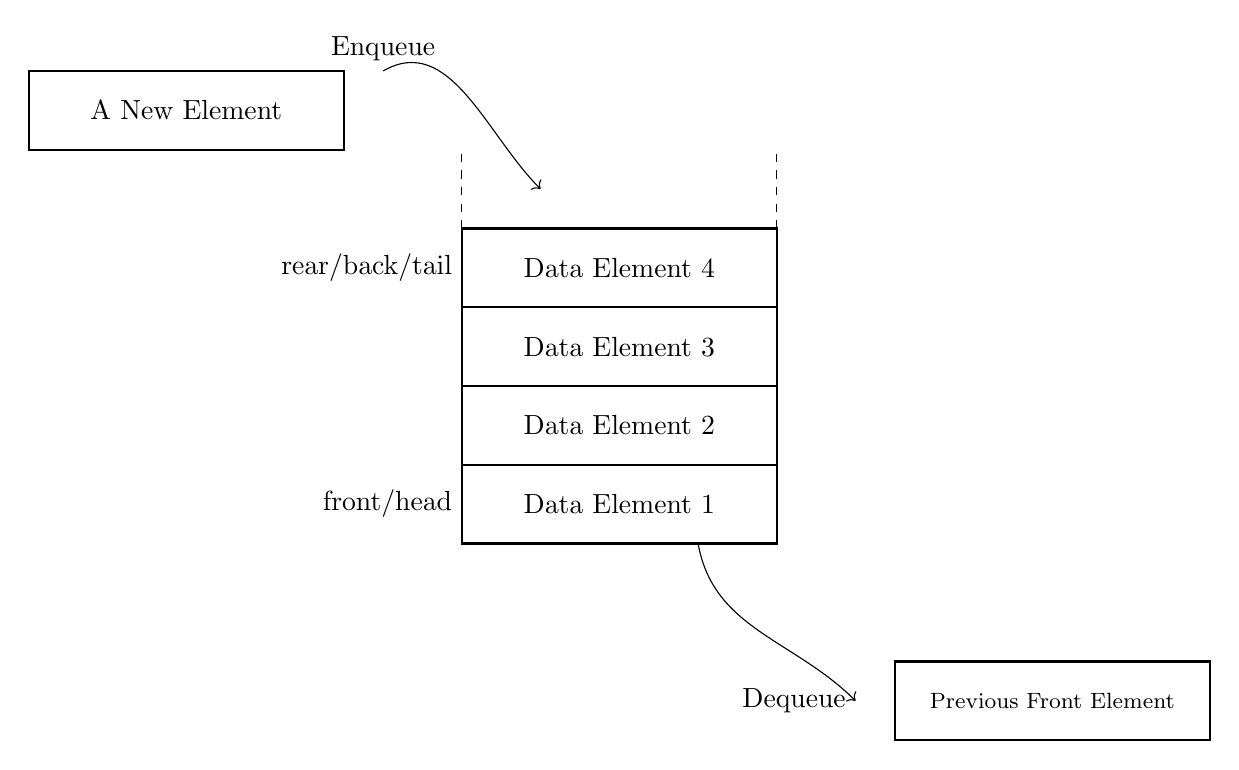
\begin{tikzpicture}
			% Stack rectangle
			\draw[thick] (-1,0) rectangle (3,4);
			\draw[thick] (-6.5,5) rectangle (-2.5,6) node[midway] {A New Element};
			\draw[thick] (4.5,-2.5) rectangle (8.5,-1.5) node[midway] {{\footnotesize Previous Front Element}};
			
			% Dividing lines 
			\draw[thick] (-1,1) -- (3,1);
			\draw[thick] (-1,2) -- (3,2);
			\draw[thick] (-1,3) -- (3,3);
			
			
			\draw[dashed] (3,4) -- (3,5);
			\draw[dashed] (-1,4) -- (-1,5);
			
			\node at (1,3.5) {Data Element 4};
			\node at (1,2.5) {Data Element 3};
			\node at (1,1.5) {Data Element 2};
			\node at (1,0.5) {Data Element 1};
			
			% Labels for top and bottom
			\node[left] at (-1,3.5) {rear/back/tail};
			\node[left] at (-1,0.5) {front/head};
			
			
			\draw[->] (-2,6) node[above] {Enqueue} to[out=+30] (0,4.5);
			
			
			\draw[->] (2,0)  to[out=-80] (4,-2) node[left] {Dequeue};
		\end{tikzpicture}
		\caption{{\footnotesize Queue Data Structure}}
		\label{fig:intro_queue}
	\end{figure}
	
	
	Queues are widely used in various applications, including:
	
	\begin{itemize}
		\item Task Scheduling: Operating systems use queues to manage processes and tasks.
		\item Print Spooling: Print jobs are queued to ensure they are processed in order.
		\item Breadth-First Search (BFS): Queues are essential in graph traversal algorithms.
		\item Buffer Management: Queues are used in networking and data streaming to manage packets.
	\end{itemize}
	
	
	
	Let's start with basic operations on queues. A queue can be implemented using an array or a linked list. Here’s how to implement a queue using a linked list in C:
	
	\begin{lstlisting}
		typedef struct Node {
			int data;
			struct Node* next;
		} Node;
		
		typedef struct Queue {
			Node* front;
			Node* rear;
		} Queue;
		
		// Create a new queue
		Queue* createQueue() {
			Queue* q = (Queue*)malloc(sizeof(Queue));
			q->front = q->rear = NULL;
			return q;
		}
		
		// Enqueue operation
		void enqueue(Queue* q, int value) {
			Node* newNode = (Node*)malloc(sizeof(Node));
			newNode->data = value;
			newNode->next = NULL;
			
			if (q->rear == NULL) {
				q->front = q->rear = newNode; // First element
				return;
			}
			q->rear->next = newNode;
			q->rear = newNode;
		}
		
		// Dequeue operation
		int dequeue(Queue* q) {
			if (q->front == NULL) {
				printf("Queue is empty\n");
				return -1; // Indicate queue is empty
			}
			Node* temp = q->front;
			int value = temp->data;
			q->front = q->front->next;
			if (q->front == NULL) {
				q->rear = NULL; // Queue is empty
			}
			free(temp);
			return value;
		}
		
		// Peek operation
		int peek(Queue* q) {
			if (q->front == NULL) {
				printf("Queue is empty\n");
				return -1; // Indicate queue is empty
			}
			return q->front->data;
		}
		
		// Check if queue is empty
		int isEmpty(Queue* q) {
			return q->front == NULL;
		}
		
		// Function to free all memory associated with the queue
		void freeQueue(Queue *q){
			while (!isEmpty(q)){
				dequeue(q); // Dequeues and frees each node
			}
			free(q); // Free the queue structure
			printf("Queue memory freed.\n");
		}
		
		int main(){
			// Create a new queue
			Queue *q = createQueue();
			
			printf("Testing the queue operations:\n");
			
			// Test isEmpty
			printf("Queue is empty? %s\n", isEmpty(q) ? "Yes" : "No");
			
			// Enqueue some elements
			printf("Enqueueing elements 10, 20, 30, 40\n");
			enqueue(q, 10);
			enqueue(q, 20);
			enqueue(q, 30);
			enqueue(q, 40);
			
			// Check isEmpty again
			printf("Queue is empty? %s\n", isEmpty(q) ? "Yes" : "No");
			
			// Peek at the front element
			printf("Front element: %d\n", peek(q));
			
			// Dequeue all elements
			printf("Dequeuing all elements:\n");
			while (!isEmpty(q)){
				printf("%d ", dequeue(q));
			}
			printf("\n");
			
			// Try to dequeue from an empty queue
			printf("Dequeueing from an empty queue:\n");
			dequeue(q);
			
			// Try to peek into an empty queue
			printf("Peeking into an empty queue: %d\n", peek(q));
			
			printf("Enqueueing elements 50, 60\n");
			enqueue(q, 50);
			enqueue(q, 60);
			
			// Peek at the front element
			printf("Front element: %d\n", peek(q));
			
			// Free the queue
			freeQueue(q);
			return 0;
		}
	\end{lstlisting}
	
	You should see in the terminal:
	
	\begin{mdframed}[style=myboxstyleTerminal1]
		\begin{verbatim}
			Testing the queue operations:
			Queue is empty? Yes
			Enqueueing elements 10, 20, 30, 40
			Queue is empty? No
			Front element: 10
			Dequeuing all elements:
			10 20 30 40 
			Dequeueing from an empty queue:
			Queue is empty
			Queue is empty
			Peeking into an empty queue: -1
			Enqueueing elements 50, 60
			Front element: 50
			Queue memory freed. 
		\end{verbatim}
	\end{mdframed}
	
	
	A \textbf{circular queue} is an advanced version of a linear queue where the last position is connected back to the first position, forming a circle. This eliminates the waste of space that can occur in a linear queue.
	
	\begin{lstlisting}
		#define SIZE 5
		
		typedef struct CircularQueue {
			int items[SIZE];
			int front;
			int rear;
		} CircularQueue;
		
		// Create a new circular queue
		CircularQueue* createCircularQueue() {
			CircularQueue* cq = (CircularQueue*)malloc(sizeof(CircularQueue));
			cq->front = -1;
			cq->rear = -1;
			return cq;
		}
		
		// Enqueue operation for circular queue
		void enqueueCircular(CircularQueue* cq, int value) {
			if ((cq->front == 0 && cq->rear == SIZE - 1) || (cq->front == cq->rear + 1)) {
				printf("Circular Queue is full\n");
				return; // Queue is full
			}
			
			if (cq->front == -1) {
				cq->front = 0; // First element
			}
			cq->rear = (cq->rear + 1) % SIZE; // Move rear to next position
			cq->items[cq->rear] = value;
		}
		
		// Dequeue operation for circular queue
		int dequeueCircular(CircularQueue* cq) {
			if (cq->front == -1) {
				printf("Circular Queue is empty\n");
				return -1; // Indicate queue is empty
			}
			
			int value = cq->items[cq->front];
			if (cq->front == cq->rear) {
				cq->front = cq->rear = -1; // Queue is empty
			} else {
				cq->front = (cq->front + 1) % SIZE; // Move front to next position
			}
			return value;
		}
		
		// Function to free memory associated with the circular queue
		void freeCircularQueue(CircularQueue *cq){
			free(cq); // Free the allocated memory
			printf("Circular queue memory freed.\n");
		}
		
		int main(){
			// Create a circular queue
			CircularQueue *cq = createCircularQueue();
			
			printf("Testing Circular Queue operations:\n");
			
			// Enqueue some elements
			printf("Enqueueing elements 10, 20, 30, 40, 50\n");
			enqueueCircular(cq, 10);
			enqueueCircular(cq, 20);
			enqueueCircular(cq, 30);
			enqueueCircular(cq, 40);
			enqueueCircular(cq, 50);
			
			// Try enqueueing when the queue is full
			printf("Attempting to enqueue 60 (should indicate full):\n");
			enqueueCircular(cq, 60);
			
			// Dequeue some elements
			printf("Dequeuing three elements:\n");
			printf("%d ", dequeueCircular(cq));
			printf("%d ", dequeueCircular(cq));
			printf("%d\n", dequeueCircular(cq));
			
			// Enqueue more elements to test wrap-around
			printf("Enqueueing elements 60, 70\n");
			enqueueCircular(cq, 60);
			enqueueCircular(cq, 70);
			
			// Dequeue all elements
			printf("Dequeuing all elements:\n");
			while (cq->front != -1){
				printf("%d ", dequeueCircular(cq));
			}
			printf("\n");
			
			// Try dequeuing when the queue is empty
			printf("Attempting to dequeue from an empty queue:\n");
			dequeueCircular(cq);
			
			// Free the circular queue
			freeCircularQueue(cq);
			return 0;
		}
	\end{lstlisting}
	
	The above test case will show:
	
	\begin{mdframed}[style=myboxstyleTerminal1]
		\begin{verbatim}
			Testing Circular Queue operations:
			Enqueueing elements 10, 20, 30, 40, 50
			Attempting to enqueue 60 (should indicate full):
			Circular Queue is full
			Dequeuing three elements:
			10 20 30
			Enqueueing elements 60, 70
			Dequeuing all elements:
			40 50 60 70 
			Attempting to dequeue from an empty queue:
			Circular Queue is empty
			Circular queue memory freed.
		\end{verbatim}
	\end{mdframed}
	
	
	A \textbf{priority queue} is an abstract data type that operates similarly to a regular queue but allows elements to be dequeued based on priority rather than order. Higher priority elements are removed before lower priority ones.
	
	\begin{lstlisting}
		#include <stdio.h>
		#include <stdlib.h>
		
		typedef struct MinHeap {
			int* arr;
			int capacity;
			int size;
		} MinHeap;
		
		MinHeap* createMinHeap(int capacity) {
			MinHeap* minHeap = (MinHeap*)malloc(sizeof(MinHeap));
			minHeap->capacity = capacity;
			minHeap->size = 0;
			minHeap->arr = (int*)malloc(capacity * sizeof(int));
			return minHeap;
		}
		
		void swap(int* a, int* b) {
			int temp = *a;
			*a = *b;
			*b = temp;
		}
		
		void insertMinHeap(MinHeap* minHeap, int value) {
			if (minHeap->size == minHeap->capacity) {
				printf("Heap is full\n");
				return;
			}
			minHeap->size++;
			int i = minHeap->size - 1;
			minHeap->arr[i] = value;
			
			while (i != 0 && minHeap->arr[(i - 1) / 2] > minHeap->arr[i]) {
				swap(&minHeap->arr[i], &minHeap->arr[(i - 1) / 2]);
				i = (i - 1) / 2;
			}
		}
		
		int removeMin(MinHeap* minHeap) {
			if (minHeap->size <= 0) {
				return -1; // Heap is empty
			}
			if (minHeap->size == 1) {
				minHeap->size--;
				return minHeap->arr[0];
			}
			
			int root = minHeap->arr[0];
			minHeap->arr[0] = minHeap->arr[minHeap->size - 1];
			minHeap->size--;
			// Heapify down
			int i = 0;
			while (i < minHeap->size / 2) {
				int smallest = i;
				if (2 * i + 1 < minHeap->size && minHeap->arr[2 * i + 1] < minHeap->arr[smallest]) {
					smallest = 2 * i + 1;
				}
				if (2 * i + 2 < minHeap->size && minHeap->arr[2 * i + 2] < minHeap->arr[smallest]) {
					smallest = 2 * i + 2;
				}
				if (smallest == i) break;
				swap(&minHeap->arr[i], &minHeap->arr[smallest]);
				i = smallest;
			}
			return root;
		}
		
		void freeMinHeap(MinHeap *minHeap){
			if (minHeap){
				free(minHeap->arr);
				free(minHeap);
			}
		}
		
		int main(){
			int capacity = 10;
			MinHeap *minHeap = createMinHeap(capacity);
			
			// Test insertions
			printf("Inserting elements into the MinHeap:\n");
			insertMinHeap(minHeap, 10);
			insertMinHeap(minHeap, 20);
			insertMinHeap(minHeap, 5);
			insertMinHeap(minHeap, 7);
			insertMinHeap(minHeap, 3);
			
			for (int i = 0; i < minHeap->size; i++){
				printf("%d ", minHeap->arr[i]);
			}
			printf("\n");
			
			// Test removals
			printf("\nRemoving elements from the MinHeap:\n");
			while (minHeap->size > 0){
				printf("Removed: %d\n", removeMin(minHeap));
				printf("Heap after removal: ");
				for (int i = 0; i < minHeap->size; i++)
				{
					printf("%d ", minHeap->arr[i]);
				}
				printf("\n");
			}
			
			// Deallocate memory
			freeMinHeap(minHeap);
			printf("\nMemory deallocated successfully.\n");
			
			return 0;
		}
		
	\end{lstlisting}
	
	The above code will print:
	
	\begin{mdframed}[style=myboxstyleTerminal1]
		\begin{verbatim}
			Inserting elements into the MinHeap:
			3 5 10 20 7 
			
			Removing elements from the MinHeap:
			Removed: 3
			Heap after removal: 5 7 10 20 
			Removed: 5
			Heap after removal: 7 20 10 
			Removed: 7
			Heap after removal: 10 20 
			Removed: 10
			Heap after removal: 20 
			Removed: 20
			Heap after removal: 
			
			Memory deallocated successfully.
		\end{verbatim}
	\end{mdframed}
	
	
	Using two stacks, you can implement a queue. The idea is to use one stack for enqueue operations and another for dequeue operations.
	
	\begin{lstlisting}
		typedef struct QueueUsingStacks {
			Stack* stack1; // For enqueue
			Stack* stack2; // For dequeue
		} QueueUsingStacks;
		
		void enqueueUsingStacks(QueueUsingStacks* q, int value) {
			push(q->stack1, value); // Push to stack1
		}
		
		int dequeueUsingStacks(QueueUsingStacks* q) {
			if (isEmpty(q->stack2)) {
				while (!isEmpty(q->stack1)) {
					// Transfer elements from stack1 to stack2
					push(q->stack2, pop(q->stack1)); 
				}
			}
			return pop(q->stack2); // Pop from stack2
		}
		
	\end{lstlisting}
	
	Write \codebox{int main} for the above code testing \codebox{QueueUsingStacks} and also create a de-allocation function. Test your program with \codebox{valgrind} to make sure there is no memory leak.
	
	
	A circular buffer can be implemented using a queue, allowing for efficient use of space and fixed-size storage. Implementing a circular buffer using a queue is an effective way to manage a fixed-size buffer. A circular buffer allows for efficient data management, especially in scenarios where data is continuously written and read, such as in streaming data applications. Below is a simple implementation of a circular buffer in C. For more practice you can write the code for a circular buffer.
	
	Queues are a fundamental data structure with a variety of applications, including scheduling, resource management, and task processing. Understanding how to implement and utilize different types of queues, such as circular queues and priority queues, equips students with valuable skills for solving real-world problems. Additionally, implementing queues using other data structures can deepen their understanding of data management and manipulation.
	
	
	
	
	
	
	
	
	
	
	
	
	
	\section{Trees}
	
	A tree is a hierarchical data structure that simulates a parent-child relationship between elements. Unlike linear data structures like arrays, linked lists, stacks, or queues, trees are non-linear and can efficiently represent relationships in a more complex manner.
	
	Trees are used in various real-world applications such as database indexing, hierarchical structures (e.g., file systems), network routing algorithms, and expression parsing in compilers. Key terminology of trees:
	
	\begin{itemize}
		\item \textbf{Node}: Basic unit containing data and references to other nodes.
		\item \textbf{Root}: The top node of the tree, from which all other nodes descend.
		\item \textbf{Parent}: A node that has children.
		\item \textbf{Child}: A node that is a descendant of another node.
		\item \textbf{Leaf}: A node that does not have any children.
		\item \textbf{Subtree}: A tree formed by a node and its descendants.
		\item \textbf{Height}: The length of the longest path from the root to a leaf.
		\item \textbf{Depth}: The number of edges from the root to a node.
		\item \textbf{Diameter} The longest path between two nodes in the tree, by counting the number of edges in between.
	\end{itemize}
	
	\begin{figure}[h!]
		\centering
		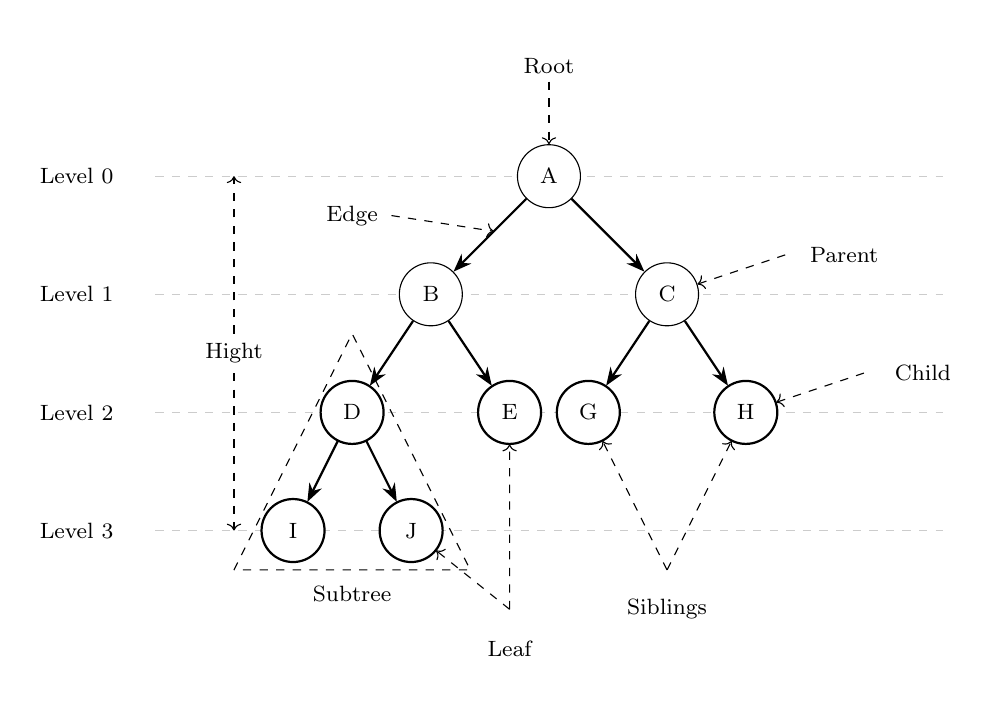
\begin{tikzpicture}[
			level distance=1.5cm,
			sibling distance=3cm,
			every node/.style={draw, fill=white, circle, minimum size=8mm, font=\footnotesize},
			edge from parent/.style={draw, thick, -{Stealth}},
			level 1/.style={sibling distance=3cm},
			level 2/.style={sibling distance=2cm},
			level 3/.style={sibling distance=1.5cm}
			]
			
			\draw[dashed, ->] (-4,-2.5) -- (-4,-4.5);
			\node[draw=none, fill=none] at (-4,-2.25) {Hight};
			\draw[dashed, ->] (-4,-2.0) -- (-4,0.0);
			
			\draw[dashed, color=black!20] (-5,0.0) -- (+5,0.0);
			\node[draw=none, fill=none] at (-6,0.0) {Level 0};
			\draw[dashed, color=black!20] (-5,-1.5) -- (+5,-1.5);
			\node[draw=none, fill=none] at (-6,-1.5) {Level 1};
			\draw[dashed, color=black!20] (-5,-3.0) -- (+5,-3.0);
			\node[draw=none, fill=none] at (-6,-3.0) {Level 2};
			\draw[dashed, color=black!20] (-5,-4.5) -- (+5,-4.5);
			\node[draw=none, fill=none] at (-6,-4.5) {Level 3};
			% Nodes of the tree
			\node (A) {A}
			child {node (B) {B} child {node (D) {D} child {node (I) {I}} child {node (J) {J}}} child {node (E) {E}}}
			child {node (C) {C}  child {node (G) {G}} child {node (H) {H }}};
			
			% Labels and descriptions
			\node[draw=none, fill=none] at (-2.5,-0.5) {Edge};
			\draw[dashed,->] (-2.5+0.5,-0.5) -- (-0.7,-0.7);
			
			\node[draw=none, fill=none, above=0.5cm of A] {Root};
			\draw[dashed,->] (0,1.2) -- (A);
			
			\draw[dashed,->] (3,-1.0) -- (C);
			\node[draw=none, fill=none] at (3+0.75,-1.0) {Parent};
			
			\draw[dashed,->] (+1.5,-5) -- (G);
			\draw[dashed,->] (+1.5,-5) -- (H);
			\node[draw=none, fill=none] at (+1.5,-5-0.5) {Siblings};
			
			\draw[dashed,->] (3+1,-2.5) -- (H);
			\node[draw=none, fill=none] at (3+1+0.75,-2.5) {Child};
			
			\draw[dashed,->] (+1.5-2,-4.5-1) -- (J);
			\draw[dashed,->] (+1.5-2,-4.5-1) -- (E);
			\node[draw=none, fill=none] at (+1.5-2,-4.5-0.5-1) {Leaf};
			
			\draw[dashed] (-4,-5) -- (-2.5,-2) -- (-1,-5) -- cycle; 
			\node[draw=none, fill=none] at (-2.5,-5.3) {Subtree};
			
		\end{tikzpicture}
		\caption{{\footnotesize Tree Data Structure}}
		\label{fig:intro_tree_structure}
	\end{figure}
	
	
	Let's start with fundamental operations like insertion, deletion, and traversal. Inserting into a binary tree typically involves finding an appropriate spot where the new node maintains the tree's properties.
	
	\begin{lstlisting}
		#include <stdio.h>
		#include <stdlib.h>
		
		typedef struct Node {
			int data;
			struct Node* left;
			struct Node* right;
		}Node;
		
		Node* createNode(int data) {
			Node* newNode = (Node*)malloc(sizeof(Node));
			newNode->data = data;
			newNode->left = newNode->right = NULL;
			return newNode;
		}
		
		void insert(Node** root, int data) {
			if (*root == NULL) {
				*root = createNode(data);
				return;
			}
			if (data < (*root)->data)
			insert(&(*root)->left, data);
			else
			insert(&(*root)->right, data);
		}
		
		void inorderTraversal(Node *root){
			if (root != NULL){
				inorderTraversal(root->left);
				printf("%d ", root->data);
				inorderTraversal(root->right);
			}
		}
		
		void deallocateTree(Node *root){
			if (root == NULL) return; 
			deallocateTree(root->left);  
			deallocateTree(root->right); 
			free(root);               
		}
		
		int main(){
			Node *root = NULL;
			insert(&root, 50);
			insert(&root, 30);
			insert(&root, 20);
			insert(&root, 40);
			insert(&root, 70);
			insert(&root, 60);
			insert(&root, 80);
			
			printf("Inorder traversal: ");
			inorderTraversal(root);
			printf("\n");
			deallocateTree(root);
			return 0;
		}
	\end{lstlisting}
	
	\begin{figure}[h!]
		\centering
		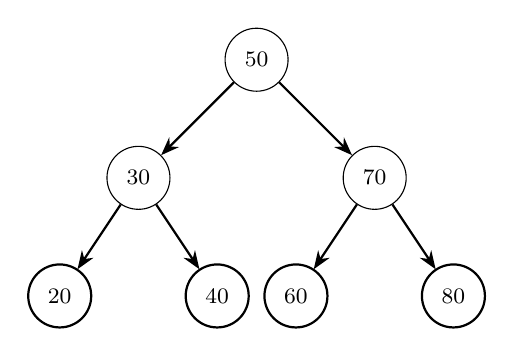
\begin{tikzpicture}[
			level distance=1.5cm,
			sibling distance=3cm,
			every node/.style={draw, fill=white, circle, minimum size=8mm, font=\footnotesize},
			edge from parent/.style={draw, thick, -{Stealth}},
			level 1/.style={sibling distance=3cm},
			level 2/.style={sibling distance=2cm},
			level 3/.style={sibling distance=1.5cm}
			]
			
			% Nodes of the tree
			\node (A) {50}
			child {node (B) {30} child {node (D) {20}} child {node (E) {40}}}
			child {node (C) {70}  child {node (G) {60}} child {node (H) {80}}};
			
			
		\end{tikzpicture}
		\caption{{\footnotesize Binary Search Tree constructed with the values 50, 30, 20, 40, 70, 60, and 80.}}
		\label{fig:intro_tree_structure_exp1}
	\end{figure}
	
	Printing the value in traversal order we have:
	
	\begin{mdframed}[style=myboxstyleTerminal1]
		\begin{verbatim}
			Inorder traversal: 20 30 40 50 60 70 80 
		\end{verbatim}
	\end{mdframed}
	
	
	
	
	
	\textbf{Inverting} a binary tree means swapping the left and right children of every node. It’s a simple yet fundamental operation. For example, Figure \ref{fig:intro_tree_structure_exp2_2} is the inverted tree for Figure \ref{fig:intro_tree_structure_exp2_1}.
	
	\begin{figure}[H]
		\centering
		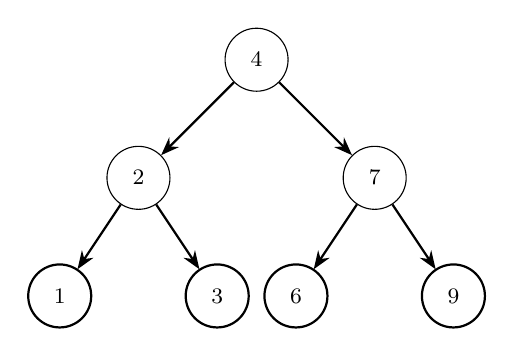
\begin{tikzpicture}[
			level distance=1.5cm,
			sibling distance=3cm,
			every node/.style={draw, fill=white, circle, minimum size=8mm, font=\footnotesize},
			edge from parent/.style={draw, thick, -{Stealth}},
			level 1/.style={sibling distance=3cm},
			level 2/.style={sibling distance=2cm},
			level 3/.style={sibling distance=1.5cm}
			]
			
			% Nodes of the tree
			\node (A) {4}
			child {node (B) {2} child {node (D) {1}} child {node (E) {3}}}
			child {node (C) {7}  child {node (G) {6}} child {node (H) {9}}};
			
			
		\end{tikzpicture}
		\caption{{\footnotesize Binary Tree Before Invert Function}}
		\label{fig:intro_tree_structure_exp2_1}
	\end{figure}
	
	
	\begin{figure}[H]
		\centering
		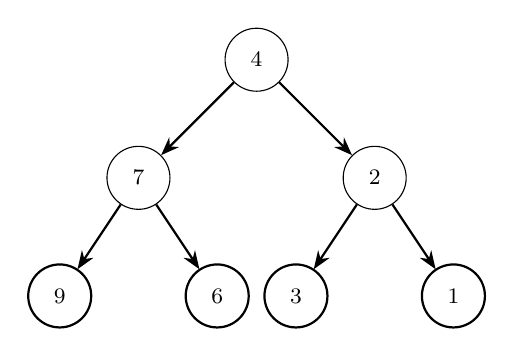
\begin{tikzpicture}[
			level distance=1.5cm,
			sibling distance=3cm,
			every node/.style={draw, fill=white, circle, minimum size=8mm, font=\footnotesize},
			edge from parent/.style={draw, thick, -{Stealth}},
			level 1/.style={sibling distance=3cm},
			level 2/.style={sibling distance=2cm},
			level 3/.style={sibling distance=1.5cm}
			]
			
			% Nodes of the tree
			\node (A) {4}
			child {node (B) {7} child {node (D) {9}} child {node (E) {6}}}
			child {node (C) {2}  child {node (G) {3}} child {node (H) {1}}};
			
			
		\end{tikzpicture}
		\caption{{\footnotesize Binary Tree After Invert Function}}
		\label{fig:intro_tree_structure_exp2_2}
	\end{figure}
	
	
	
	The C code to invert a Binary Tree is shown below here. What do you think should be de-allocated after calling \codebox{invertTree}? 
	
	\begin{lstlisting}
		Node* invertTree(Node* root) {
			if (root == NULL) return NULL;
			struct Node* temp = root->left;
			root->left = root->right;
			root->right = temp;
			
			invertTree(root->left);
			invertTree(root->right);
			return root;
		}
		
	\end{lstlisting}
	
	
	The \textbf{depth} of a binary tree is the longest path from the root to a leaf node. It can be calculated recursively by checking the height of the left and right subtrees and returning the greater of the two.
	
	\begin{lstlisting}
		int maxDepth(Node* root) {
			if (root == NULL) return 0;
			int leftDepth = maxDepth(root->left);
			int rightDepth = maxDepth(root->right);
			return (leftDepth > rightDepth ? leftDepth : rightDepth) + 1;
		}
		
	\end{lstlisting}
	
	
	The \textbf{diameter} of a binary tree is the length of the longest path between two nodes in a tree. This path may or may not pass through the root.
	
	\begin{lstlisting}
		int diameter(Node* root, int* height) {
			if (root == NULL) {
				*height = 0;
				return 0;
			}
			
			int leftHeight = 0, rightHeight = 0;
			int leftDiameter = diameter(root->left, &leftHeight);
			int rightDiameter = diameter(root->right, &rightHeight);
			
			*height = (leftHeight > rightHeight ? leftHeight : rightHeight) + 1;
			return fmax(leftHeight + rightHeight + 1, fmax(leftDiameter, rightDiameter));
		}
	\end{lstlisting}
	
	
	A Binary Search Tree is a binary tree where each node follows the rule:
	
	\begin{itemize}
		\item The value of the left child is less than the value of the parent.
		\item The value of the right child is greater than the value of the parent.
	\end{itemize}
	
	BSTs are useful for searching and sorting operations, offering average time complexity of $O(log n)$ for search, insert, and delete operations.
	
	
	A \textbf{balanced} binary tree is one in which the height difference between the left and right subtrees of any node is at most one. This ensures optimal time complexity for insertion, deletion, and search operations. To check if a tree is balanced:
	
	\begin{lstlisting}
		int isBalanced(Node* root) {
			if (root == NULL) return 1;
			
			int leftHeight = maxDepth(root->left);
			int rightHeight = maxDepth(root->right);
			
			return abs(leftHeight - rightHeight) <= 1 && isBalanced(root->left) && isBalanced(root->right);
		}
	\end{lstlisting}
	
	
	
	Trees are a versatile and foundational data structure in computer science. From basic operations like insertion and traversal to more advanced operations like tree inversion and depth calculation, they are used in various real-world applications such as databases, file systems, and algorithms. By mastering binary trees and their specialized forms like Binary Search Trees (BST) and Balanced Trees, students can efficiently solve many computational problems.
	
	
	
	
	
	\section{Tries}
	
	A Trie, often referred to as a prefix tree, is a specialized tree data structure that is particularly well-suited for managing a dynamic set of strings, where the keys are usually strings. The term "Trie" is derived from the word "retrieval." Tries are designed to facilitate fast lookups, insertions, and deletions of keys while providing efficient storage. Some key characteristics of tries:
	
	\begin{itemize}
		\item \textbf{Structure}: A Trie consists of nodes, where each node represents a character of a string. The path from the root to a particular node represents a prefix of some strings stored in the Trie.
		\item \textbf{Root Node}: The root node is usually empty and serves as the starting point for all strings.
		\item \textbf{Children Nodes}: Each node can have multiple children corresponding to different characters.
		\item \textbf{End of Word}: A boolean flag is typically associated with nodes to indicate whether a particular node marks the end of a valid word.
	\end{itemize}
	
	\begin{figure}[h!]
		\centering
		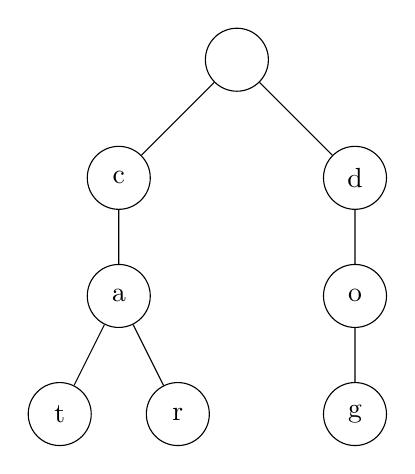
\begin{tikzpicture}[
			level 1/.style={sibling distance=30mm},
			level 2/.style={sibling distance=15mm},
			every node/.style={circle, draw, minimum size=8mm, inner sep=1mm}
			]
			\node { }
			child { node {c}
				child { node {a}
					child { node {t} }
					child { node {r} }
				}
			}
			child { node {d}
				child { node {o}
					child { node {g} }
				}
			};
		\end{tikzpicture}
		\caption{{\footnotesize Trie structure representing "cat", "car", and "dog".}}
		\label{fig:intro_trie_structure_exp1}
	\end{figure}
	
	Applications of Tries are:
	
	\begin{itemize}
		\item \textbf{ Autocomplete Systems}: Tries are widely used in search engines and text editors to provide suggestions as users type.
		\item \textbf{Spell Checkers}: They help quickly verify whether a word exists in a dictionary.
		\item \textbf{IP Routing}: Tries can be used to store and search routing prefixes efficiently.
		\item \textbf{Longest Common Prefix}: They can be used to find the longest common prefix among a set of strings.
	\end{itemize}
	
	Let's start we basic implementations. To insert a string into a Trie, start from the root and traverse down the tree, creating nodes as necessary for each character in the string. Once the last character is inserted, mark that node as the end of a word.
	
	\begin{lstlisting}
		#define ALPHABET_SIZE 26
		
		typedef struct TrieNode {
			struct TrieNode *children[ALPHABET_SIZE];
			bool isEndOfWord;
		} TrieNode;
		
		TrieNode *getNode(){
			TrieNode *node = (TrieNode *)malloc(sizeof(TrieNode));
			node->isEndOfWord = false;
			for (int i = 0; i < ALPHABET_SIZE; i++)
			node->children[i] = NULL;
			return node;
		}
		
		void insert(TrieNode *root, const char *key){ // "apple"
			TrieNode *pCrawl = root;
			for (int level = 0; key[level] != '\0'; level++){
				int index = key[level] - 'a'; // Assuming lowercase letters
				if (!pCrawl->children[index])
				pCrawl->children[index] = getNode();
				pCrawl = pCrawl->children[index];
			}
			pCrawl->isEndOfWord = true; // Mark end of word
		}
		
		void freeTrie(TrieNode *root){
			if (root == NULL){
				return;
			}
			for (int i = 0; i < ALPHABET_SIZE; i++){
				if (root->children[i] != NULL){
					freeTrie(root->children[i]);
				}
			}
			free(root);
		}
		
		int main(){
			TrieNode *root = getNode();
			
			// Insert keys into the Trie
			insert(root, "apple");
			insert(root, "app");
			insert(root, "ape");
			insert(root, "bat");
			insert(root, "batman");
			insert(root, "batter");
			
			freeTrie(root);
		}
	\end{lstlisting}
	
	The the above code will create the data structure shown in Figure \ref{fig:intro_tree_structure_exp2_1} from (a) to (f).
	
	
	\begin{figure}[h!]
		\centering
		
		% Subplot 1
		\begin{subfigure}[t]{0.45\textwidth}
			\centering
			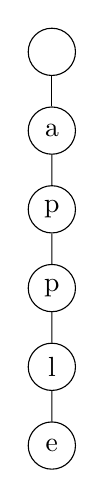
\begin{tikzpicture}[
				level distance=10mm,
				sibling distance=12mm,
				every node/.style={circle, draw, minimum size=6mm, inner sep=1mm}
				]
				\node {}
				child { node {a}
					child { node {p}
						child { node {p}
							child { node {l}
								child { node {e} }
							}
						}
					}
				};
			\end{tikzpicture}
			\caption{= "apple"}
		\end{subfigure}
		\hfill
		% Subplot 2
		\begin{subfigure}[t]{0.45\textwidth}
			\centering
			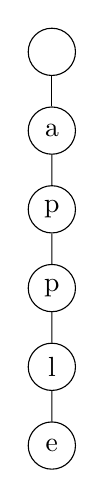
\begin{tikzpicture}[
				level distance=10mm,
				sibling distance=12mm,
				every node/.style={circle, draw, minimum size=6mm, inner sep=1mm}
				]
				\node {}
				child { node {a}
					child { node {p}
						child { node {p}
							child { node {l}
								child { node {e} }
							}
						}
					}
				};
			\end{tikzpicture}
			\caption{= (a) + "app"}
		\end{subfigure}
		
		\vspace{10pt}
		
		% Subplot 3
		\begin{subfigure}[t]{0.45\textwidth}
			\centering
			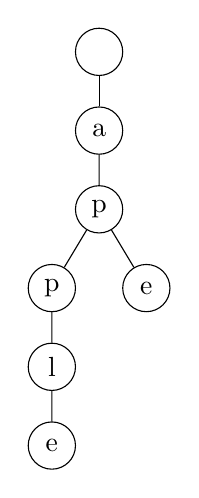
\begin{tikzpicture}[
				level distance=10mm,
				sibling distance=12mm,
				every node/.style={circle, draw, minimum size=6mm, inner sep=1mm}
				]
				\node {}
				child { node {a}
					child { node {p}
						child { node {p}
							child { node {l}
								child { node {e} }
							}
						}
						child { node {e} }
					}
				};
				
			\end{tikzpicture}
			\caption{= (b) + "ape"}
		\end{subfigure}
		\hfill
		% Subplot 4
		\begin{subfigure}[t]{0.45\textwidth}
			\centering
			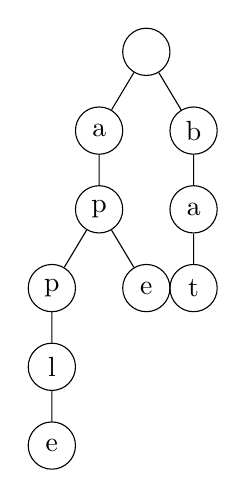
\begin{tikzpicture}[
				level distance=10mm,
				sibling distance=12mm,
				every node/.style={circle, draw, minimum size=6mm, inner sep=1mm}
				]
				\node {}
				child { node {a}
					child { node {p}
						child { node {p}
							child { node {l}
								child { node {e} }
							}
						}
						child { node {e} }
					}
				}
				child { node {b}
					child { node {a}
						child { node {t} }
					}
				};
				
			\end{tikzpicture}
			\caption{= (c) + "bat"}
		\end{subfigure}
		
		\vspace{10pt}
		
		% Subplot 5
		\begin{subfigure}[t]{0.45\textwidth}
			\centering
			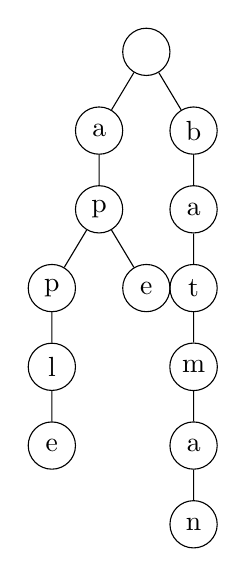
\begin{tikzpicture}[
				level distance=10mm,
				sibling distance=12mm,
				every node/.style={circle, draw, minimum size=6mm, inner sep=1mm}
				]
				\node {}
				child { node {a}
					child { node {p}
						child { node {p}
							child { node {l}
								child { node {e} }
							}
						}
						child { node {e} }
					}
				}
				child { node {b}
					child { node {a}
						child { node {t}
							child { node {m}
								child { node {a}
									child { node {n} }
								}
							}
						}
					}
				};
				
				
			\end{tikzpicture}
			\caption{= (d) + "batman"}
		\end{subfigure}
		\hfill
		% Subplot 6
		\begin{subfigure}[t]{0.45\textwidth}
			\centering
			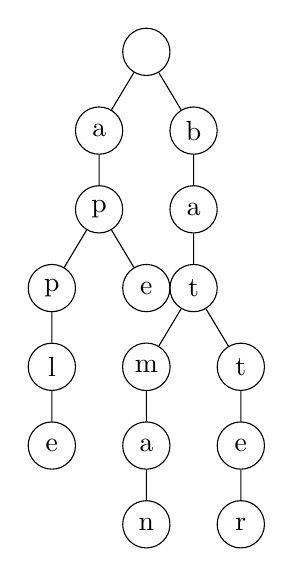
\begin{tikzpicture}[
				level distance=10mm,
				sibling distance=12mm,
				every node/.style={circle, draw, minimum size=6mm, inner sep=1mm}
				]
				\node {}
				child { node {a}
					child { node {p}
						child { node {p}
							child { node {l}
								child { node {e} }
							}
						}
						child { node {e} }
					}
				}
				child { node {b}
					child { node {a}
						child { node {t}
							child { node {m}
								child { node {a}
									child { node {n} }
								}
							}
							child { node {t}
								child { node {e}
									child { node {r} }
								}
							}
						}
					}
				};
				
			\end{tikzpicture}
			\caption{= (e) + "batter"}
		\end{subfigure}
		
		\caption{{\footnotesize Creating a Trie holding the words "apple", "app", "ape", "bat", "batman", "batter" added in order.}}
		\label{fig:trie_subplots}
	\end{figure}
	
	To \textbf{search} for a string in a Trie, follow the path defined by the characters of the string. If you reach a node that signifies the end of the string and the end of the word flag is true, then the string exists in the Trie.
	
	\begin{lstlisting}
		bool search(TrieNode *root, const char *key){
			TrieNode *pCrawl = root;
			for (int level = 0; key[level] != '\0'; level++){
				int index = key[level] - 'a';
				if (!pCrawl->children[index])
				return false;
				pCrawl = pCrawl->children[index];
			}
			return (pCrawl != NULL && pCrawl->isEndOfWord);
		}
	\end{lstlisting}
	
	
	\textbf{Deletion} is slightly more complex. To delete a string, you need to traverse down the tree as you would for searching. If the end of the word is reached, unmark the end of the word flag. If the node has no children, you can remove the node and backtrack.
	
	\begin{lstlisting}
		bool isEmptyNode(TrieNode *node) {
			for (int i = 0; i < ALPHABET_SIZE; i++) {
				if (node->children[i] != NULL) {
					return false;
				}
			}
			return true;
		}
		
		bool deleteHelper(TrieNode *root, const char *key, int depth) {
			if (!root) return false;
			
			if (depth == strlen(key)) {
				if (root->isEndOfWord) {
					root->isEndOfWord = false;
				}
				if (isEmptyNode(root)) {
					free(root);
					return true;  // Node can be deleted.
				}
				return false;
			}
			
			int index = key[depth] - 'a';
			if (deleteHelper(root->children[index], key, depth + 1)) {
				root->children[index] = NULL;
				if (!root->isEndOfWord && isEmptyNode(root)) {
					free(root);
					return true;  // Propagate deletion.
				}
			}
			return false;
		}
		
		void deleteKey(TrieNode *root, const char *key){
			deleteHelper(root, key, 0);
		}	
	\end{lstlisting}
	
	
	Using a Trie for \textbf{autocomplete} functionality involves finding all the words that share a common prefix.
	
	\begin{lstlisting}
		void printSuggestions(TrieNode *root, char *prefix){
			if (root->isEndOfWord)
			printf("%s\n", prefix);
			
			for (int i = 0; i < ALPHABET_SIZE; i++){
				if (root->children[i]){
					char newPrefix[100];
					snprintf(newPrefix, sizeof(newPrefix), "%s%c", prefix, 'a' + i);
					printSuggestions(root->children[i], newPrefix);
				}
			}
		}
		
		void autocomplete(TrieNode *root, const char *prefix){
			TrieNode *pCrawl = root;
			for (int level = 0; prefix[level] != '\0'; level++){
				int index = prefix[level] - 'a';
				if (!pCrawl->children[index])
				return; // No suggestions
				pCrawl = pCrawl->children[index];
			}
			printSuggestions(pCrawl, (char *)prefix);
		}
	\end{lstlisting}
	
	To find the \textbf{longest common prefix} among an array of strings using a Trie, you can insert all the strings into the Trie and then traverse the Trie until you hit a node with multiple children or the end of a word.
	
	\begin{lstlisting}
		char *longestCommonPrefix(TrieNode *root){
			TrieNode *pCrawl = root;
			char *prefix = (char *)malloc(100);
			int index = 0;
			
			while (pCrawl && !pCrawl->isEndOfWord){
				int childCount = 0;
				int childIndex = -1;
				for (int i = 0; i < ALPHABET_SIZE; i++){
					if (pCrawl->children[i]){
						childCount++;
						childIndex = i;
					}
				}
				if (childCount != 1)
				break; // More than one child, stop
				prefix[index++] = 'a' + childIndex;
				pCrawl = pCrawl->children[childIndex];
			}
			prefix[index] = '\0';
			return prefix;
		}
	\end{lstlisting}
	
	You can use the following \codebox{main} to test the above functions:
	
	\begin{lstlisting}
		int main(){
			TrieNode *root = getNode();
			
			// Insert keys into the Trie
			insert(root, "apple");
			insert(root, "app");
			insert(root, "ape");
			insert(root, "bat");
			insert(root, "batman");
			insert(root, "batter");
			
			// Search for keys
			printf("Searching 'app': %s\n", search(root, "app") ? "Found" : "Not Found");
			printf("Searching 'bat': %s\n", search(root, "bat") ? "Found" : "Not Found");
			printf("Searching 'cat': %s\n", search(root, "cat") ? "Found" : "Not Found");
			
			// Autocomplete suggestions for prefix "ba"
			printf("Autocomplete suggestions for 'ba':\n");
			autocomplete(root, "ba");
			
			// Longest common prefix
			char *prefix = longestCommonPrefix(root);
			printf("Longest common prefix: %s\n", prefix);
			free(prefix);
			
			// Delete a key and search again
			deleteKey(root, "bat");
			printf("Searching 'bat' after deletion: %s\n", search(root, "bat") ? "Found" : "Not Found");
			
			// Free allocated memory
			freeTrie(root);
		}
	\end{lstlisting}
	
	
	
	Tries are a powerful data structure for managing strings and implementing efficient search functionalities. Understanding how to insert, search, delete, and utilize tries for advanced operations such as autocomplete and finding the longest common prefix will equip students with valuable skills for handling string-related challenges in programming. Tries can outperform other data structures in certain scenarios, especially when dealing with large sets of strings or when prefix-based queries are common.
	
	
	
	
	\section{Heap}
	
	A heap is a specialized binary tree-based data structure that satisfies the heap property. Heaps are useful for implementing priority queues and for efficient sorting algorithms such as Heapsort. There are two types of heaps:
	
	\begin{itemize}
		\item Max-Heap: In a max-heap, the key of a parent node is always greater than or equal to the keys of its children.
		
		\begin{figure}[h!]
			\centering
			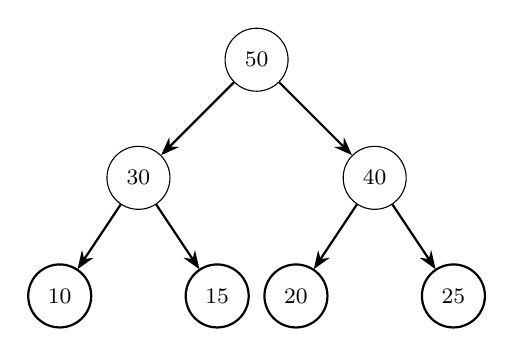
\begin{tikzpicture}[
				level distance=1.5cm,
				sibling distance=3cm,
				every node/.style={draw, fill=white, circle, minimum size=8mm, font=\footnotesize},
				edge from parent/.style={draw, thick, -{Stealth}},
				level 1/.style={sibling distance=3cm},
				level 2/.style={sibling distance=2cm},
				level 3/.style={sibling distance=1.5cm}
				]
				
				% Nodes of the tree
				\node (A) {50}
				child {node (B) {30} child {node (D) {10}} child {node (E) {15}}}
				child {node (C) {40}  child {node (G) {20}} child {node (H) {25}}};
				
				
			\end{tikzpicture}
			\caption{{\footnotesize Max Heap}}
			\label{fig:HeapMax}
		\end{figure}
		
		
		\item Min-Heap: In a min-heap, the key of a parent node is always less than or equal to the keys of its children.
		
		\begin{figure}[h!]
			\centering
			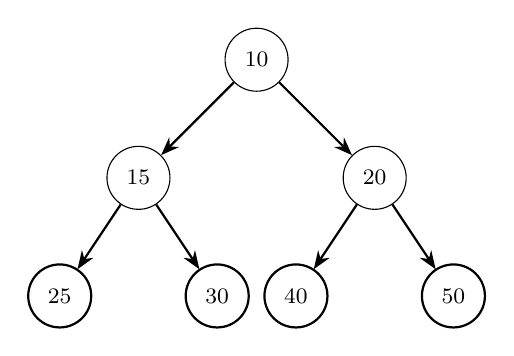
\begin{tikzpicture}[
				level distance=1.5cm,
				sibling distance=3cm,
				every node/.style={draw, fill=white, circle, minimum size=8mm, font=\footnotesize},
				edge from parent/.style={draw, thick, -{Stealth}},
				level 1/.style={sibling distance=3cm},
				level 2/.style={sibling distance=2cm},
				level 3/.style={sibling distance=1.5cm}
				]
				
				% Nodes of the tree
				\node (A) {10}
				child {node (B) {15} child {node (D) {25}} child {node (E) {30}}}
				child {node (C) {20}  child {node (G) {40}} child {node (H) {50}}};
				
				
			\end{tikzpicture}
			\caption{{\footnotesize Min Heap}}
			\label{fig:HeapMin}
		\end{figure}
		
		
	\end{itemize}
	
	The main advantage of using a heap is its ability to maintain the heap property during insertion and deletion operations in logarithmic time, making it suitable for tasks like scheduling and event simulation. Some of heap applications are:
	
	\begin{itemize}
		\item \textbf{Priority Queues}: Heaps are often used to implement priority queues, where the highest (or lowest) priority element is retrieved first.
		\item \textbf{Heapsort}: Heaps provide an efficient way to sort an array in-place with a time complexity of $O(nlog n)$.
		\item \textbf{Graph Algorithm}s: Heaps are used in algorithms like Dijkstra’s shortest path algorithm and Prim’s minimum spanning tree algorithm.
		\item \textbf{Memory Management}: Heaps are used to manage memory allocation dynamically.
	\end{itemize}
	
	
	Before we start programming heaps, it is necessary to understand the basic concepts, including:
	
	\begin{enumerate}
		\item \textbf{Complete Binary Tree}: A heap is a complete binary tree, meaning all levels are completely filled except possibly for the last level, which is filled from left to right.
		\item \textbf{Heap Property}: For a max-heap, the key at each node must be greater than or equal to the keys of its children, and for a min-heap, the key at each node must be less than or equal to the keys of its children.
		\item \textbf{Heap Representation}: Heaps are often implemented using arrays rather than linked structures. The parent-child relationships are managed using simple arithmetic:
		\begin{itemize}
			\item Parent of node at index $i$: $Parent(i) = \dfrac{i-1}{2}$
			\item Left child of node at index $i$: $Left(i) = 2i+1$
			\item Right child of node at index $i$: $Right(i) = 2i+2$
		\end{itemize}
	\end{enumerate}
	
	
	Heapify is the process used to restore the heap property after insertion or deletion. The two main operations are:
	
	\begin{enumerate}
		\item \textbf{Heapify up}: Restores the heap property after insertion.
		\item \textbf{Heapify down}: Restores the heap property after deletion of the root.
	\end{enumerate}
	
	Inserting an element into a max-heap requires placing the new element at the end of the heap (at the next available leaf position). Then, the element is moved up the tree until the heap property is restored, a process known as \textbf{heapifying up}. Here is a basic implementation of insertion in a max-heap:
	
	\begin{lstlisting}
		#include <stdio.h>
		#include <stdlib.h>
		
		#define MAX 100
		
		typedef struct {
			int array[MAX];
			int size;
		} MaxHeap;
		
		MaxHeap* createHeap() {
			MaxHeap* heap = (MaxHeap*)malloc(sizeof(MaxHeap));
			heap->size = 0;
			return heap;
		}
		
		void heapifyUp(MaxHeap* heap, int index) {
			int parentIndex = (index - 1) / 2;
			if (index > 0 && heap->array[index] > heap->array[parentIndex]) {
				// Swap with parent
				int temp = heap->array[index];
				heap->array[index] = heap->array[parentIndex];
				heap->array[parentIndex] = temp;
				heapifyUp(heap, parentIndex);
			}
		}
		
		void insert(MaxHeap* heap, int value) {
			if (heap->size == MAX) {
				printf("Heap is full!\n");
				return;
			}
			// Insert at the end
			heap->array[heap->size] = value;
			heap->size++;
			// Heapify up
			heapifyUp(heap, heap->size - 1);
		}
		
		void printHeap(MaxHeap* heap) {
			for (int i = 0; i < heap->size; i++) {
				printf("%d ", heap->array[i]);
			}
			printf("\n");
		}
		
		int main() {
			MaxHeap* heap = createHeap();
			insert(heap, 10);
			insert(heap, 20);
			insert(heap, 5);
			insert(heap, 30);
			insert(heap, 15);
			
			printHeap(heap); // Output: 30 20 5 10 15
			free(heap);
			return 0;
		}
		
	\end{lstlisting}
	
	\textbf{Deletion} in a max-heap usually involves removing the root node (the largest element in the max-heap). After removal, the last element in the heap replaces the root, and the heap is \textbf{heapified down} to maintain the heap property.
	
	\begin{lstlisting}
		void heapifyDown(MaxHeap* heap, int index) {
			int left = 2 * index + 1;
			int right = 2 * index + 2;
			int largest = index;
			
			if (left < heap->size && heap->array[left] > heap->array[largest]) {
				largest = left;
			}
			if (right < heap->size && heap->array[right] > heap->array[largest]) {
				largest = right;
			}
			if (largest != index) {
				// Swap
				int temp = heap->array[index];
				heap->array[index] = heap->array[largest];
				heap->array[largest] = temp;
				heapifyDown(heap, largest);
			}
		}
		
		int deleteRoot(MaxHeap* heap) {
			if (heap->size == 0) {
				printf("Heap is empty!\n");
				return -1;
			}
			
			int rootValue = heap->array[0];
			heap->array[0] = heap->array[heap->size - 1];
			heap->size--;
			heapifyDown(heap, 0);
			
			return rootValue;
		}
	\end{lstlisting}
	
	Test the above delectation function with adding following the following code into the \codebox{main} function:
	
	\begin{lstlisting}
		printf("\nDeleting root element (max value): %d\n", deleteRoot(heap));
		printf("Heap after deleting root: ");
		printHeap(heap); // Output: 20 15 5 10
	\end{lstlisting}
	
	\textbf{Heapsort} is an efficient, comparison-based sorting algorithm that leverages the heap data structure. The algorithm has a time complexity of $O(nlog n)$ and works by building a max-heap from the input data, then repeatedly extracting the maximum element and rebuilding the heap.
	
	\begin{lstlisting}
		void heapSort(int array[], int size) {
			MaxHeap* heap = createHeap();
			
			// Build the heap
			for (int i = 0; i < size; i++) {
				insert(heap, array[i]);
			}
			
			// Extract elements one by one
			for (int i = size - 1; i >= 0; i--) {
				array[i] = deleteRoot(heap);
			}
			free(heap);
		}
	\end{lstlisting}
	
	Test the above \codebox{heapSort} with:
	
	\begin{lstlisting}
		int arr[] = {5, 2, 9, 1, 5, 6};
		int size = sizeof(arr) / sizeof(arr[0]);
		printf("\nOriginal array: ");
		for (int i = 0; i < size; i++) {
			printf("%d ", arr[i]);
		}
		printf("\n");
		
		heapSort(arr, size);
		
		printf("Array after heap sort: ");
		for (int i = 0; i < size; i++) {
			printf("%d ", arr[i]);
		}
		printf("\n");
	\end{lstlisting} 
	
	
	The problem \textbf{Kth Largest Element in a Stream} requires maintaining a running stream of numbers and being able to efficiently retrieve the Kth largest element after every new insertion. This problem can be efficiently solved using a min-heap (also known as a priority queue). We use a \textbf{min-heap} of size $k$, where the smallest element in the heap is the Kth largest element. The approach we need to take is:
	
	\begin{enumerate}
		\item We maintain a min-heap of size $k$.
		\item Each time a new number is added:
		\begin{itemize}
			\item If the heap has fewer than $k$ elements, we insert the number.
			\item If the heap already contains $k$ elements, we compare the new number with the root (smallest element in the heap). If the new number is larger, we replace the root with the new number and reheapify.
		\end{itemize}
		
		\item The root of the heap will always contain the Kth largest element.
	\end{enumerate}
	
	
	Here's how we can implement the above steps in C:
	
	\begin{lstlisting}
		#define MAX 100
		typedef struct{
			int *array;
			int size;
			int capacity;
		} MinHeap;
		
		MinHeap *createMinHeap(int capacity){
			MinHeap *heap = (MinHeap *)malloc(sizeof(MinHeap));
			heap->array = (int *)malloc(sizeof(int) * capacity);
			heap->size = 0;
			heap->capacity = capacity;
			return heap;
		}
		
		void swap(int *a, int *b){
			int temp = *a;
			*a = *b;
			*b = temp;
		}
		
		void heapifyDown(MinHeap *heap, int index){
			int left = 2 * index + 1;
			int right = 2 * index + 2;
			int smallest = index;
			
			if (left < heap->size && heap->array[left] < heap->array[smallest]){
				smallest = left;
			}
			if (right < heap->size && heap->array[right] < heap->array[smallest]){
				smallest = right;
			}
			if (smallest != index){
				swap(&heap->array[index], &heap->array[smallest]);
				heapifyDown(heap, smallest);
			}
		}
		
		void heapifyUp(MinHeap *heap, int index){
			int parent = (index - 1) / 2;
			if (index > 0 && heap->array[index] < heap->array[parent]){
				swap(&heap->array[index], &heap->array[parent]);
				heapifyUp(heap, parent);
			}
		}
		
		void insert(MinHeap *heap, int value){
			if (heap->size < heap->capacity){
				heap->array[heap->size] = value;
				heap->size++;
				heapifyUp(heap, heap->size - 1);
			}
			else if (value > heap->array[0]){
				heap->array[0] = value;
				heapifyDown(heap, 0);
			}
		}
		
		int getKthLargest(MinHeap *heap){
			return heap->array[0]; // The root of the min-heap is the Kth largest element.
		}
		
		int main(){
			int k = 3;
			MinHeap *heap = createMinHeap(k);
			
			int stream[] = {4, 5, 8, 2, 6, 9};
			int n = sizeof(stream) / sizeof(stream[0]);
			
			for (int i = 0; i < n; i++){
				insert(heap, stream[i]);
				if (heap->size == k){
					printf("After inserting %d, the %d-th largest element is: %d\n", stream[i], k, getKthLargest(heap));
				}
			}
			
			free(heap->array);
			free(heap);
			return 0;
		}
	\end{lstlisting}
	
	We maintain a heap of size $k$, where every insertion ensures that the Kth largest element is always at the root. For example, if $k=3$, after inserting numbers 4, 5, 8, 2, 6, and 9 into the stream, the program will print the 3rd largest number after each insertion where the heap reaches size $k$.
	
	The problem \textbf{Merge k Sorted Lists} requires merging $k$ sorted linked lists into a single sorted linked list. A min-heap can help solve this problem efficiently. The basic idea is to repeatedly extract the smallest element from all the lists until all the lists are empty. First, we push the first element of each list into a min-heap.
	Then, we extract the smallest element from the heap, append it to the merged list, and then insert the next element from the same list into the heap. Repeat this process until all lists are exhausted. Here is the implementation in C:
	
	\begin{lstlisting}
		#include <stdio.h>
		#include <stdlib.h>
		
		// Definition for singly-linked list.
		typedef struct ListNode{
			int val;
			struct ListNode *next;
		} ListNode;
		
		typedef struct {
			ListNode **array;
			int size;
		} MinHeap;
		
		// Create a new linked list node
		ListNode *createNode(int val){
			ListNode *newNode = (ListNode *)malloc(sizeof(ListNode));
			newNode->val = val;
			newNode->next = NULL;
			return newNode;
		}
		
		// Swap two list nodes in heap
		void swap(ListNode **a, ListNode **b){
			ListNode *temp = *a;
			*a = *b;
			*b = temp;
		}
		
		// Heapify down
		void heapifyDown(MinHeap *heap, int i){
			int left = 2 * i + 1;
			int right = 2 * i + 2;
			int smallest = i;
			
			if (left < heap->size && heap->array[left]->val < heap->array[smallest]->val){
				smallest = left;
			}
			if (right < heap->size && heap->array[right]->val < heap->array[smallest]->val){
				smallest = right;
			}
			if (smallest != i){
				swap(&heap->array[i], &heap->array[smallest]);
				heapifyDown(heap, smallest);
			}
		}
		
		// Insert into the heap
		void insertHeap(MinHeap *heap, ListNode *node){
			heap->array[heap->size] = node;
			heap->size++;
			
			// Heapify up
			int i = heap->size - 1;
			int parent = (i - 1) / 2;
			while (i > 0 && heap->array[i]->val < heap->array[parent]->val){
				swap(&heap->array[i], &heap->array[parent]);
				i = parent;
				parent = (i - 1) / 2;
			}
		}
		
		// Extract min from heap
		ListNode *extractMin(MinHeap *heap){
			if (heap->size == 0){
				return NULL;
			}
			ListNode *root = heap->array[0];
			heap->array[0] = heap->array[heap->size - 1];
			heap->size--;
			heapifyDown(heap, 0);
			return root;
		}
		
		// Function to merge k sorted lists
		ListNode *mergeKLists(ListNode **lists, int k){
			MinHeap heap;
			heap.array = (ListNode **)malloc(sizeof(ListNode *) * k);
			heap.size = 0;
			
			// Insert first node of each list into the heap
			for (int i = 0; i < k; i++){
				if (lists[i] != NULL){
					insertHeap(&heap, lists[i]);
				}
			}
			
			// Create a dummy node for the merged list
			ListNode *dummy = createNode(0);
			ListNode *tail = dummy;
			
			// Extract min and insert next node from the list
			while (heap.size > 0){
				ListNode *minNode = extractMin(&heap);
				tail->next = minNode;
				tail = minNode;
				if (minNode->next != NULL){
					insertHeap(&heap, minNode->next);
				}
			}
			
			ListNode *result = dummy->next;
			free(dummy);  // Free the dummy node
			free(heap.array);  // Free the heap array
			return result;
		}
		
		// Helper function to print the list
		void printList(ListNode *head){
			while (head != NULL){
				printf("%d -> ", head->val);
				head = head->next;
			}
			printf("NULL\n");
		}
		
		// Function to free the entire linked list
		void freeList(ListNode *head){
			while (head != NULL){
				ListNode *temp = head;
				head = head->next;
				free(temp);
			}
		}
		
		int main(){
			// Create test cases
			ListNode *l1 = createNode(1);
			l1->next = createNode(4);
			l1->next->next = createNode(5);
			
			ListNode *l2 = createNode(1);
			l2->next = createNode(3);
			l2->next->next = createNode(4);
			
			ListNode *l3 = createNode(2);
			l3->next = createNode(6);
			
			ListNode *lists[] = {l1, l2, l3};
			
			// Merge k sorted lists
			ListNode *mergedList = mergeKLists(lists, 3);
			// Output: 1 -> 1 -> 2 -> 3 -> 4 -> 4 -> 5 -> 6 -> NULL
			printList(mergedList); 
			
			// Free the memory allocated for all lists
			freeList(mergedList);
			
			return 0;
		}
		
	\end{lstlisting}
	
	For more practice, find a problem that uses max heap. Heaps are an essential data structure for priority management and efficient sorting. Their use extends across algorithms that require fast retrieval of the minimum or maximum value, with applications in priority queues, graph algorithms, and even memory management systems.
	
	
	
	
	
	
	\section{Graphs}
	
	A graph is a powerful and versatile data structure used to represent relationships between different entities. A graph is defined as a set of \textbf{vertices} (also called nodes) connected by \textbf{edges}. The vertices represent entities, and the edges represent the relationships or connections between them. Graphs are used extensively in computer science for modeling real-world systems such as networks (social networks, computer networks), maps (GPS systems), and many optimization problems (e.g., shortest path).
	
	
	Graphs are classified into several types based on their properties:
	
	\begin{itemize}
		\item \textbf{Undirected Graph}: The edges have no direction. For example, if there is an edge between vertex A and vertex B, you can traverse it in both directions.
		\item \textbf{Directed Graph (Digraph)}: The edges have directions. An edge from vertex A to vertex B does not imply an edge from B to A.
		\item \textbf{Weighted Graph}: The edges have weights or costs associated with them. Weighted graphs are often used in problems that require finding the shortest path or the minimum cost.
	\end{itemize}
	
	Graphs can be represented in two primary ways:
	
	\begin{enumerate}
		\item \textbf{Adjacency Matrix}: A 2D array is used where \codebox{matrix[i][j] = 1} (or the weight of the edge) if there is an edge from vertex \codebox{i} to vertex \codebox{j}.
		\item \textbf{Adjacency List}: Each vertex has a list of adjacent vertices (i.e., vertices that are directly connected to it by an edge). This representation is more space-efficient for sparse graphs.
	\end{enumerate}
	
	
	
	
	
	\begin{figure}[h!]
		\centering
		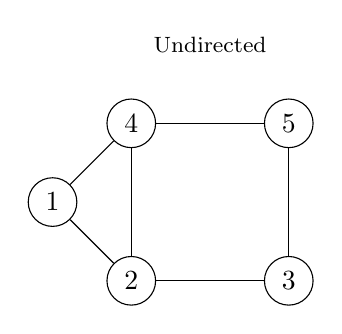
\begin{tikzpicture}
			\node at (2,2) {{\footnotesize Undirected}};
			\node[circle, draw] (A) at (0,0) {1};
			\node[circle, draw] (B) at (1,-1) {2};
			\node[circle, draw] (C) at (3,-1) {3};
			\node[circle, draw] (D) at (1, 1) {4};
			\node[circle, draw] (E) at (3, 1) {5};
			
			\draw (A) -- (B);
			\draw (B) -- (D);
			\draw (A) -- (D);
			\draw (D) -- (E);
			\draw (B) -- (C);
			\draw (C) -- (E);		
			
		\end{tikzpicture}
		\hspace{5cm}
		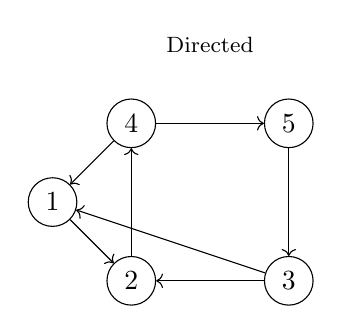
\begin{tikzpicture}
			\node at (2,2) {{\footnotesize Directed}};
			\node[circle, draw] (A) at (0,0) {1};
			\node[circle, draw] (B) at (1,-1) {2};
			\node[circle, draw] (C) at (3,-1) {3};
			\node[circle, draw] (D) at (1, 1) {4};
			\node[circle, draw] (E) at (3, 1) {5};
			
			\draw[->] (A) -- (B);
			\draw[->] (B) -- (D);
			\draw[->] (C) -- (A);
			\draw[->] (C) -- (B);
			\draw[->] (D) -- (A);
			\draw[->] (D) -- (E);
			\draw[->] (E) -- (C);
			
			
		\end{tikzpicture}
		
		\vspace{1cm}
		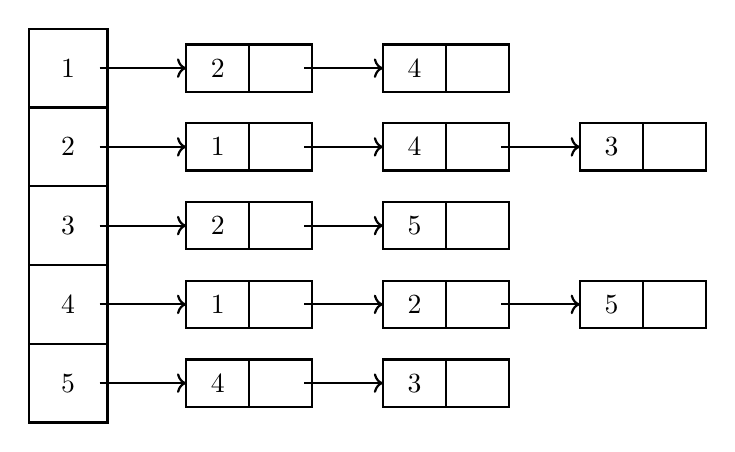
\begin{tikzpicture}
			
			\draw[thick] (4.5,-2.5) rectangle (5.5,2.5);
			\node at (5,2) {1};
			\draw[thick] (4.5,1.5) -- (5.5,1.5);
			\node at (5,1) {2};
			\draw[thick] (4.5,0.5) -- (5.5,0.5);
			\node at (5,0) {3};
			\draw[thick] (4.5,-0.5) -- (5.5,-0.5);
			\node at (5,-1) {4};
			\draw[thick] (4.5,-1.5) -- (5.5,-1.5);
			\node at (5,-2) {5};
			
			\draw[->, thick] (5.4,2) -- (6.5,2);
			\draw[thick] (6.5,1.7) rectangle (8.1,2.3);
			\draw[thick] (7.3,1.7) -- (7.3,2.3);
			\node at (6.9,2) {2};
			\draw[->, thick] (8,2) -- (9,2);
			\draw[thick] (9,1.7) rectangle (10.6,2.3);
			\draw[thick] (9.8,1.7) -- (9.8,2.3);.
			\node at (9.4,2) {4};
			
			
			
			\draw[->, thick] (5.4,1) -- (6.5,1);
			\draw[thick] (6.5,0.7) rectangle (8.1,1.3);
			\draw[thick] (7.3,0.7) -- (7.3,1.3);
			\node at (6.9,1) {1};
			\draw[->, thick] (8,1) -- (9,1);
			\draw[thick] (9,0.7) rectangle (10.6,1.3);
			\draw[thick] (9.8,0.7) -- (9.8,1.3);
			\node at (9.4,1) {4};
			\draw[->, thick] (10.5,1) -- (11.5,1);
			\draw[thick] (11.5,0.7) rectangle (13.1,1.3);
			\draw[thick] (12.3,0.7) -- (12.3,1.3);.
			\node at (11.9,1) {3};
			
			\draw[->, thick] (5.4,0) -- (6.5,0);
			\draw[thick] (6.5,-0.3) rectangle (8.1,0.3);
			\draw[thick] (7.3,-0.3) -- (7.3,0.3);
			\node at (6.9,0) {2};
			\draw[->, thick] (8,0) -- (9,0);
			\draw[thick] (9,-0.3) rectangle (10.6,0.3);
			\draw[thick] (9.8,-0.3) -- (9.8,0.3);
			\node at (9.4,0) {5};
			
			
			\draw[->, thick] (5.4,-1) -- (6.5,-1);
			\draw[thick] (6.5,-1.3) rectangle (8.1,-0.7);
			\draw[thick] (7.3,-1.3) -- (7.3,-0.7);
			\node at (6.9,-1) {1};
			\draw[->, thick] (8,-1) -- (9,-1);
			\draw[thick] (9,-1.3) rectangle (10.6,-0.7);
			\draw[thick] (9.8,-1.3) -- (9.8,-0.7);
			\node at (9.4,-1) {2};
			\draw[->, thick] (10.5,-1) -- (11.5,-1);
			\draw[thick] (11.5,-1.3) rectangle (13.1,-0.7);
			\draw[thick] (12.3,-1.3) -- (12.3,-0.7);.
			\node at (11.9,-1) {5};
			
			
			\draw[->, thick] (5.4,-2) -- (6.5,-2);
			\draw[thick] (6.5,-2.3) rectangle (8.1,-1.7);
			\draw[thick] (7.3,-2.3) -- (7.3,-1.7);
			\node at (6.9,-2) {4};
			\draw[->, thick] (8,-2) -- (9,-2);
			\draw[thick] (9,-2.3) rectangle (10.6,-1.7);
			\draw[thick] (9.8,-2.3) -- (9.8,-1.7);
			\node at (9.4,-2) {3};
		\end{tikzpicture}
		\hspace{1cm}
		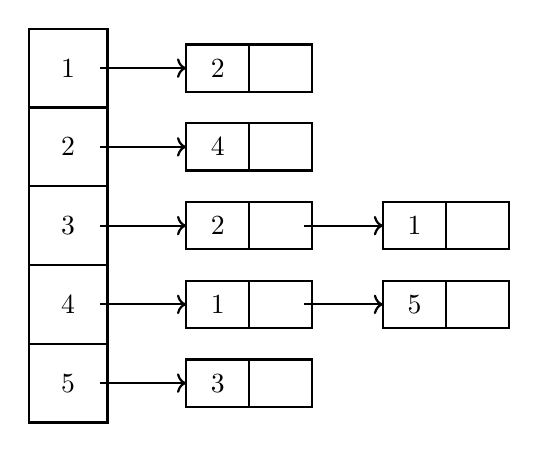
\begin{tikzpicture}
			
			\draw[thick] (4.5,-2.5) rectangle (5.5,2.5);
			\node at (5,2) {1};
			\draw[thick] (4.5,1.5) -- (5.5,1.5);
			\node at (5,1) {2};
			\draw[thick] (4.5,0.5) -- (5.5,0.5);
			\node at (5,0) {3};
			\draw[thick] (4.5,-0.5) -- (5.5,-0.5);
			\node at (5,-1) {4};
			\draw[thick] (4.5,-1.5) -- (5.5,-1.5);
			\node at (5,-2) {5};
			
			\draw[->, thick] (5.4,2) -- (6.5,2);
			\draw[thick] (6.5,1.7) rectangle (8.1,2.3);
			\draw[thick] (7.3,1.7) -- (7.3,2.3);
			\node at (6.9,2) {2};
			
			\draw[->, thick] (5.4,1) -- (6.5,1);
			\draw[thick] (6.5,0.7) rectangle (8.1,1.3);
			\draw[thick] (7.3,0.7) -- (7.3,1.3);
			\node at (6.9,1) {4};
			
			\draw[->, thick] (5.4,0) -- (6.5,0);
			\draw[thick] (6.5,-0.3) rectangle (8.1,0.3);
			\draw[thick] (7.3,-0.3) -- (7.3,0.3);
			\node at (6.9,0) {2};
			\draw[->, thick] (8,0) -- (9,0);
			\draw[thick] (9,-0.3) rectangle (10.6,0.3);
			\draw[thick] (9.8,-0.3) -- (9.8,0.3);
			\node at (9.4,0) {1};
			
			
			\draw[->, thick] (5.4,-1) -- (6.5,-1);
			\draw[thick] (6.5,-1.3) rectangle (8.1,-0.7);
			\draw[thick] (7.3,-1.3) -- (7.3,-0.7);
			\node at (6.9,-1) {1};
			\draw[->, thick] (8,-1) -- (9,-1);
			\draw[thick] (9,-1.3) rectangle (10.6,-0.7);
			\draw[thick] (9.8,-1.3) -- (9.8,-0.7);
			\node at (9.4,-1) {5};
			
			
			\draw[->, thick] (5.4,-2) -- (6.5,-2);
			\draw[thick] (6.5,-2.3) rectangle (8.1,-1.7);
			\draw[thick] (7.3,-2.3) -- (7.3,-1.7);
			\node at (6.9,-2) {3};
		\end{tikzpicture}
		
		
		\vspace{1cm}
		
		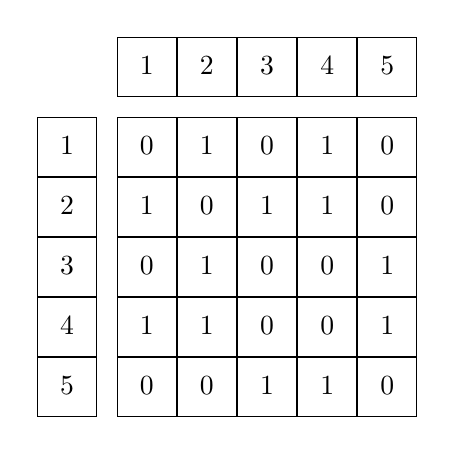
\begin{tikzpicture}
			% First matrix (column vector)
			\matrix[matrix of nodes, nodes in empty cells, nodes={draw, anchor=center, text height=1.5ex, text depth=.25ex, minimum size=0.75cm}] (m1) {
				1 \\
				2 \\
				3 \\
				4 \\
				5 \\
			};
			
			% Second matrix (adjacency matrix), placed to the right of the first matrix
			\matrix[matrix of nodes, nodes in empty cells, nodes={draw, anchor=center, text height=1.5ex, text depth=.25ex, minimum size=0.75cm}] (m2) [right=0cm of m1] {
				0 & 1 & 0 & 1 & 0 \\
				1 & 0 & 1 & 1 & 0 \\
				0 & 1 & 0 & 0 & 1 \\
				1 & 1 & 0 & 0 & 1 \\
				0 & 0 & 1 & 1 & 0 \\
			};
			
			\matrix[matrix of nodes, nodes in empty cells, nodes={draw, anchor=center, text height=1.5ex, text depth=.25ex, minimum size=0.75cm}] (m3) [above=0cm of m2] {
				1 & 2 & 3 & 4 & 5 \\
			};
		\end{tikzpicture}
		\hspace{3cm}
		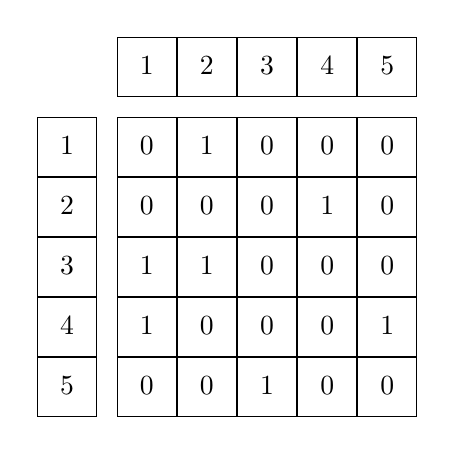
\begin{tikzpicture}
			% First matrix (column vector)
			\matrix[matrix of nodes, nodes in empty cells, nodes={draw, anchor=center, text height=1.5ex, text depth=.25ex, minimum size=0.75cm}] (m1) {
				1 \\
				2 \\
				3 \\
				4 \\
				5 \\
			};
			
			% Second matrix (adjacency matrix), placed to the right of the first matrix
			\matrix[matrix of nodes, nodes in empty cells, nodes={draw, anchor=center, text height=1.5ex, text depth=.25ex, minimum size=0.75cm}] (m2) [right=0cm of m1] {
				0 & 1 & 0 & 0 & 0 \\
				0 & 0 & 0 & 1 & 0 \\
				1 & 1 & 0 & 0 & 0 \\
				1 & 0 & 0 & 0 & 1 \\
				0 & 0 & 1 & 0 & 0 \\
			};
			
			\matrix[matrix of nodes, nodes in empty cells, nodes={draw, anchor=center, text height=1.5ex, text depth=.25ex, minimum size=0.75cm}] (m3) [above=0cm of m2] {
				1 & 2 & 3 & 4 & 5 \\
			};
		\end{tikzpicture}
		
		\caption{{\footnotesize Undirected and Directed Graphs with Adjacency List and Matrix Representation}}
		\label{fig:Graph}
	\end{figure}
	
	Let's try an example using Adjacency List in C:
	
	\begin{lstlisting}
		#include <stdio.h>
		#include <stdlib.h>
		
		// Structure to represent a node in the adjacency list
		struct Node{
			int vertex;
			struct Node *next;
		};
		
		// Structure to represent an adjacency list
		struct Graph{
			int numVertices;
			struct Node **adjLists;
		};
		
		// Create a node
		struct Node *createNode(int v){
			struct Node *newNode = malloc(sizeof(struct Node));
			newNode->vertex = v;
			newNode->next = NULL;
			return newNode;
		}
		
		// Create a graph
		struct Graph *createGraph(int vertices){
			struct Graph *graph = malloc(sizeof(struct Graph));
			graph->numVertices = vertices;
			graph->adjLists = malloc(vertices * sizeof(struct Node *));
			for (int i = 0; i < vertices; i++)
			graph->adjLists[i] = NULL;
			
			return graph;
		}
		
		// Add edge
		void addEdge(struct Graph *graph, int src, int dest){
			struct Node *newNode = createNode(dest);
			newNode->next = graph->adjLists[src];
			graph->adjLists[src] = newNode;
			
			// Since it's an undirected graph, add an edge from dest to src also
			newNode = createNode(src);
			newNode->next = graph->adjLists[dest];
			graph->adjLists[dest] = newNode;
		}
		
		// Print the graph
		void printGraph(struct Graph *graph){
			for (int v = 0; v < graph->numVertices; v++){
				struct Node *temp = graph->adjLists[v];
				printf("Vertex %d\n: ", v);
				while (temp){
					printf("%d -> ", temp->vertex);
					temp = temp->next;
				}
				printf("\n");
			}
		}
		
		// Function to free the memory allocated for the graph
		void freeGraph(struct Graph *graph){
			// Free all the nodes in the adjacency list
			for (int i = 0; i < graph->numVertices; i++){
				struct Node *temp = graph->adjLists[i];
				while (temp)
				{
					struct Node *next = temp->next;
					free(temp);  // Free the current node
					temp = next; // Move to the next node
				}
			}
			
			// Free the adjacency list array
			free(graph->adjLists);
			
			// Free the graph structure
			free(graph);
		}
		
		int main(){
			int vertices = 5;
			struct Graph *graph = createGraph(vertices);
			
			addEdge(graph, 0, 1);
			addEdge(graph, 0, 4);
			addEdge(graph, 1, 4);
			addEdge(graph, 1, 3);
			addEdge(graph, 1, 2);
			addEdge(graph, 2, 3);
			addEdge(graph, 3, 4);
			
			printGraph(graph);
			
			// Free the graph memory
			freeGraph(graph);
			return 0;
		}
	\end{lstlisting}
	
	
	Graph traversal is the process of visiting all the vertices in a graph. There are two primary algorithms for traversing graphs:
	
	\begin{enumerate}
		\item \textbf{Depth-First Search (DFS)}: This algorithm starts at a vertex and explores as far as possible along each branch before backtracking. It uses a stack (or recursion). The code below here is an example of implementing DFS in C:
		
		\begin{lstlisting}
			#include <stdio.h>
			#include <stdlib.h>
			
			#define MAX 100
			
			int visited[MAX] = {0};
			
			// DFS function
			void DFS(int vertex, int adjMatrix[][MAX], int numVertices) {
				visited[vertex] = 1;
				printf("Visited %d\n", vertex);
				
				for (int i = 0; i < numVertices; i++) {
					if (adjMatrix[vertex][i] == 1 && !visited[i]) {
						DFS(i, adjMatrix, numVertices);
					}
				}
			}
			
			int main() {
				int numVertices = 5;
				int adjMatrix[MAX][MAX] = { {0, 1, 0, 1, 0},
					{1, 0, 1, 0, 1},
					{0, 1, 0, 1, 0},
					{1, 0, 1, 0, 1},
					{0, 1, 0, 1, 0} };
				
				DFS(0, adjMatrix, numVertices);
				
				return 0;
			}
		\end{lstlisting}
		
		\item \textbf{Breadth-First Search (BFS)}: This algorithm starts at a vertex and explores all of its neighbors before moving to the next level of neighbors. It uses a queue. Here is a C implementation of BFS in C:
		
		\begin{lstlisting}
			#include <stdio.h>
			#include <stdlib.h>
			
			#define MAX 100
			
			int queue[MAX], front = -1, rear = -1;
			int visited[MAX] = {0};
			
			// Enqueue function
			void enqueue(int vertex) {
				if (rear == MAX - 1)
				return;
				if (front == -1)
				front = 0;
				rear++;
				queue[rear] = vertex;
			}
			
			// Dequeue function
			int dequeue() {
				if (front == -1)
				return -1;
				int vertex = queue[front];
				if (front == rear)
				front = rear = -1;
				else
				front++;
				return vertex;
			}
			
			// BFS function
			void BFS(int startVertex, int adjMatrix[][MAX], int numVertices) {
				visited[startVertex] = 1;
				enqueue(startVertex);
				
				while (front != -1) {
					int currentVertex = dequeue();
					printf("Visited %d\n", currentVertex);
					
					for (int i = 0; i < numVertices; i++) {
						if (adjMatrix[currentVertex][i] == 1 && !visited[i]) {
							enqueue(i);
							visited[i] = 1;
						}
					}
				}
			}
			
			int main() {
				int numVertices = 5;
				int adjMatrix[MAX][MAX] = { {0, 1, 0, 1, 0},
					{1, 0, 1, 0, 1},
					{0, 1, 0, 1, 0},
					{1, 0, 1, 0, 1},
					{0, 1, 0, 1, 0} };
				
				BFS(0, adjMatrix, numVertices);
				
				return 0;
			}
		\end{lstlisting}
	\end{enumerate}
	
	
	Graphs have a wide range of applications, and as students become more familiar with basic concepts, they can explore more advanced topics. Below are some crucial advanced topics that students need to understand:
	
	\begin{enumerate}
		\item \textbf{Topological Sorting}: This algorithm is used to order the vertices of a \textbf{Directed Acyclic Graph (DAG)} in a linear sequence where for every directed edge u → v, vertex u comes before vertex v in the ordering. Topological sorting is commonly used in scenarios like task scheduling, where certain tasks must be performed before others.
		\item \textbf{Dijkstra’s Algorithm}: This is a \textbf{single-source shortest path algorithm} for finding the shortest paths from a source vertex to all other vertices in a weighted graph, where all the edge weights are non-negative. It uses a greedy approach and is widely applied in routing and pathfinding problems, like in GPS systems.
		\item \textbf{Minimum Spanning Tree (MST)}: An MST is a subset of the edges of a graph that connects all the vertices with the minimum possible total edge weight. Two well-known algorithms to find MSTs are Kruskal’s Algorithm and Prim’s Algorithm. This problem is useful in network design, where the goal is to minimize the total length of cables required to connect all computers in a network.
		\item \textbf{Floyd-Warshall Algorithm}: This algorithm is used for finding the shortest paths between all pairs of vertices in a graph. Unlike Dijkstra’s, which only finds the shortest path from a single source, Floyd-Warshall calculates the shortest path between every pair of nodes. It works even for graphs with negative edge weights (but no negative cycles).
		\item \textbf{Bellman-Ford Algorithm}: Like Dijkstra’s algorithm, Bellman-Ford is also used for finding the shortest paths from a single source. The major difference is that Bellman-Ford works even when some of the edge weights are negative. However, it is slower than Dijkstra’s and is commonly used when negative edge weights are present.
		\item \textbf{Bipartite Graphs}: A \textbf{bipartite} graph is a graph whose vertices can be divided into two disjoint sets such that no two vertices within the same set are adjacent. This concept is widely used in matching problems, where you need to match elements from two different sets, such as job applicants to jobs, or students to projects.
		\item \textbf{Graph Coloring}: Graph coloring is the process of assigning colors to the vertices of a graph such that no two adjacent vertices share the same color. It is a well-known problem in scheduling and register allocation in compilers.
	\end{enumerate}
	
	Graphs are an essential topic in computer science, offering numerous applications in both theoretical and practical domains. Mastering the various algorithms associated with graphs can open up new problem-solving techniques for a wide range of computational challenges. Understanding graph representations, traversal techniques, and advanced algorithms will equip you with the skills to handle complex problems efficiently.
	
	
	
	
	
	
	\section*{Supplementary Exercises}
	
	
	\begin{enumerate}[label=\textbf{\arabic*}.,leftmargin=2em]
		
		\item Create a Hash Table \codebox{struc} with a string key and a floating-point data. Write \codebox{insert()} to save data with given format in the following \codebox{main}. Develop a searching function for a key and \textbf{return} the corresponding data (\codebox{search()}). Essentially de-allocate the memory for \codebox{hashTable} with \codebox{freeTable()}. You can use a the \codebox{hashFunction(char *str)} given in the lecture notes.
		
		\textit{Example}:
		
		\begin{lstlisting}[basicstyle=\scriptsize]
			#define TABLE_SIZE 10
			
			unsigned long hashFunction(char *str){
				unsigned long hash = 5381;
				int c;
				while ((c = *str++)){
					hash = ((hash << 5) + hash) + c; // hash << 5 = hash * 2^5
				}
				return hash % TABLE_SIZE;
			}
			
			int main(){
				HashEntry **hashTable = calloc(TABLE_SIZE, sizeof(HashEntry*));
				
				insert(hashTable, "apple", 0.3);
				insert(hashTable, "banana", 1.1);
				insert(hashTable, "orange", 0.9);
				
				printf("Protein in 'orange': %0.1lf\n", search(hashTable, "orange"));
				printf("Protein in 'cherry': %0.1lf\n", search(hashTable, "cherry"));
				
				freeTable(hashTable);
			}
			
		\end{lstlisting}
		
		
		\begin{itemize}
			\item \textit{Input}: \codebox{"apple"}, \codebox{"banana"}, and \codebox{"orange"} are the \textbf{keys}, while \codebox{0.3}, \codebox{1.1}, and \codebox{0.9} are their corresponding values.
			
			\item \textit{Explanation}: The output of the above code:
			
			{\footnotesize \begin{mdframed}[style=myboxstyleTerminal1]
					\begin{verbatim}
						Protein in 'orange': 0.9
						Protein in 'cherry': -1.0
					\end{verbatim}
			\end{mdframed}}
		\end{itemize}
		
		
		
		
		
		\item Create a Linked List with inserting (\codebox{appendNode()}) and printing (\codebox{printList()}) the node functions, and freeing the allocated memory (\codebox{freeList()}).
		
		\textit{Example 1}:
		
		\begin{lstlisting}
			// Main function
			int main(){
				Node *head = NULL;
				
				// Inserting nodes
				appendNode(&head, "red");
				appendNode(&head, "blue");
				appendNode(&head, "green");
				
				// Printing the list
				printList(head);
				
				// Free the memory
				freeList(head);
			}
			
		\end{lstlisting}
		
		\begin{itemize}
			\item \textit{Input}: \codebox{"red"} ,\codebox{"blue"}, and \codebox{"green"} are input data. The size of this string can range from short to quite large.
			
			\item \textit{Explanation}: The above code will print the following list:
			
			\begin{mdframed}[style=myboxstyleTerminal1]
				\begin{verbatim}
					green -> blue -> red -> NULL
				\end{verbatim}
			\end{mdframed}
		\end{itemize}
		
		
		
		\textit{IMPORTANT NOTES}:
		\begin{itemize}
			\item Adding a new data must be done with $O(1)$ time complexity.
			\item Memory allocation is required for each node and for each piece of data stored as a string.
		\end{itemize}
		
		
		
		\item Solve the following problems from \textbf{LeetCode}:
		
		\begin{enumerate}
			\item Hash Map:
			\begin{itemize}
				\item \href{https://leetcode.com/problems/two-sum/description/}{Two Sum}
				\item \href{https://leetcode.com/problems/contains-duplicate/}{Contains Duplicate}
				\item \href{https://leetcode.com/problems/top-k-frequent-elements/description/}{Top K Frequent Elements}
			\end{itemize}
			
			\item Linked List: 
			\begin{itemize}
				\item \href{https://leetcode.com/problems/add-two-numbers/}{Add Two Numbers}
				\item \href{https://leetcode.com/problems/copy-list-with-random-pointer/}{Copy List With Random Pointer}
				\item \href{https://leetcode.com/problems/lru-cache/description/}{LRU Cache}
			\end{itemize}
			
			\item Stack:
			\begin{itemize}
				\item \href{https://leetcode.com/problems/evaluate-reverse-polish-notation/description/}{Evaluate Reverse Polish Notation}
				\item \href{https://leetcode.com/problems/daily-temperatures/}{Daily Temperatures}
			\end{itemize}
			
			\item Queues: 
			\begin{itemize}
				\item \href{https://leetcode.com/problems/implement-queue-using-stacks/description/}{Implement Queue using Stacks}
				\item \href{https://leetcode.com/problems/implement-stack-using-queues/description/}{Implement Stack using Queues} 
				\item \href{https://leetcode.com/problems/orderly-queue/description/}{Orderly Queue}
				\item \href{https://leetcode.com/problems/n-queens/description/}{N-Queens}
			\end{itemize}
			
			\item Trees:
			\begin{itemize}
				\item \href{https://leetcode.com/problems/subtree-of-another-tree/}{Subtree of Another Tree} 
				\item \href{https://leetcode.com/problems/kth-smallest-element-in-a-bst/description/}{Kth Smallest Element in a BST}
				\item \href{https://leetcode.com/problems/binary-tree-maximum-path-sum/}{Binary Tree Maximum Path Sum}
			\end{itemize}
			
			\item Tries:
			\begin{itemize}
				\item \href{https://leetcode.com/problems/word-break/description/}{Word Break}
				\item \href{https://leetcode.com/problems/replace-words/description/}{Replace Words}
				\item \href{https://leetcode.com/problems/word-search-ii/}{Word Search II}
			\end{itemize}
			
			\item Heap:
			\begin{itemize}
				\item \href{https://leetcode.com/problems/task-scheduler/description/}{Task Scheduler} 
				\item \href{https://leetcode.com/problems/design-twitter/description/}{Design Twitter} 
			\end{itemize}
			
			\item Graph:
			\begin{itemize}
				\item \href{https://leetcode.com/problems/number-of-islands/}{Number of Islands} 
				\item \href{https://leetcode.com/problems/clone-graph/description/}{Clone Graph}
				\item \href{https://leetcode.com/problems/course-schedule/}{Course Schedule}
				\item \href{https://leetcode.com/problems/pacific-atlantic-water-flow/}{Pacific Atlantic Water Flow}
				\item \href{https://leetcode.com/problems/surrounded-regions/}{Surrounded Regions}
			\end{itemize}
			
			
		\end{enumerate}
		
		
	\end{enumerate}
	
	
	
	
	
	
	
	
	
	
	
	
	
	
	
	
	
	
	
	\chapter{Parallel Computing}
	
	\section*{Introduction}
	
	Parallel computing is a paradigm that enables the simultaneous execution of multiple tasks, breaking them down into smaller sub-tasks that can be performed concurrently. This approach contrasts with traditional sequential computing, where tasks are executed one after another. Parallel computing is a response to the growing demand for increased computational power to tackle complex problems in science, engineering, and other fields. In this chapter, we just discuss basics of Parallel Computing. If you want to learn more about it, study \href{http://www.cas.mcmaster.ca/~nedialk/COURSES/HPSC/node9.html}{High Performance Parallel Computing} by Prof. Ned Nedialkov.
	
	\section{Getting Started}
	
	Consider a simple operation where you want to compute the sum of two vectors \codebox{a} and \codebox{b} element-wise:
	
	\begin{lstlisting}
		for (int i = 0; i < m; i++) {
			x[i] = a[i] + b[i];
		}
	\end{lstlisting}
	% create the picture of ...
	In this loop, \codebox{m} operations are performed sequentially. The time $t_1$ is taken to execute this loop on a single processor. If we have $p$ processors, we can distribute the workload among them. Each processor handles a portion of the array elements, performing the same operation in parallel. The time taken $t_p$ on pp processors is given by:
	
	$$t_p = \frac{t_1}{p}$$
	
	This is based on the assumption that the workload can be perfectly divided among the processors, and there is no overhead in coordinating their work. In practice, achieving perfect parallelism can be challenging due to issues like load imbalance and communication overhead.
	
	First, we need to distribute segments of arrays $a$, $b$, and $x$ among the processors. For example, if you have 4 processors, each processor gets $\frac{m}{4}$ elements of $a$, $b$, and $x$. Each processor performs the addition independently on its segment of the arrays. After the parallel execution, results from all processors need to be combined to get the final result $x$.
	
	Take the following loop for example
	
	\begin{lstlisting}
		for (int i = 0; i < m; i++){
			x[i + 1] = a[i] * x[i] + b[i];
		}
	\end{lstlisting}
	
	It cannot be parallelized straightforwardly due to a dependency between iterations. Each iteration depends on the result of the previous one (\codebox{x[i+1]} depends on \codebox{x[i]}), creating a data dependency. This is often referred to as a "loop-carried dependency."
	
	
	Understanding the computer architecture is crucial for effective parallel computing. Here's an overview of key components and their interplay:
	
	\begin{enumerate}
		\item \textbf{Registers}: Registers are small, fast storage locations within the CPU. Instructions and data are typically loaded into registers for processing. They provide extremely fast access but have limited capacity.
		
		\item \textbf{Caches}:
		\begin{itemize}
			
			\item \textbf{L1 cache} is the first level of cache and is usually on the same chip as the processor cores. It has a small capacity but offers very fast access. It stores frequently accessed instructions and data. It's divided into separate instruction and data caches.
			
			\item \textbf{L2 cache} is larger but slightly slower than L1.
			It serves as a backup to L1, providing additional space for frequently used data.
			Located either on the same chip as the processor or very close.
			
			\item Some systems have an \textbf{L3 cache} shared among multiple cores or processors.
			
		\end{itemize}
		
		\item \textbf{Memory (RAM)}: RAM (Random Access Memory) is the primary memory of a computer. It has a much larger capacity compared to caches but is slower. When data isn't found in the cache, it's fetched from RAM.
		
	\end{enumerate}
	
	
	
	Data moves through this hierarchy, with the fastest and smallest storage (registers) at the top and the largest but slowest (memory) at the bottom. Registers are the fastest storage but have the least capacity. Then, L1 cache is faster than L2, and L2 is faster than RAM. When data is initially accessed, it's brought from main memory to cache. Subsequent accesses to the same data might benefit from the faster cache access, if the data is in cache.
	
	Data isn't transferred between memory and cache one byte at a time; instead, it's done in blocks known as cache lines. A cache line is typically 64 or 128 bytes. This helps utilize spatial locality — if one part of data is accessed, it's likely that nearby data will be accessed soon. All information I have mentioned here about computer architecture in my Linux OS can be seen by \codebox{lscpu} or \codebox{cat /proc/cpuinfo}.
	
	Let's have an example of matrix multiplication. Previous we called the following matrix multiplication algorithm \textbf{Naive-MMM}:
	
	\begin{lstlisting}
		double **MatrixMultiplication(double **A,double **B, int Arows, int Acols, int Brows, int Bcols){
			// check if the condition is ok
			if (Acols!=Brows){
				printf("ERROR: The dimension does not match for matrix multiplication.\n");
				return NULL;
			}
			
			double **C = allocate2Darray(Arows, Bcols);
			if (C==NULL){
				return NULL;
			}
			
			for (int i = 0; i < Arows; i++){ // Arows is now the Crows
				for (int j = 0; j < Bcols; j++){ // Bcols is now the Ccols
					double sum = 0;
					for (int k = 0; k < Acols; k++){ // Acols is equal to Brows
						sum += A[i][k] * B[k][j];
					}
					C[i][j] = sum;
				}
			}
			
			return C;
		}
	\end{lstlisting} 
	
	We can implement the exact same matrix multiplication (with the same time complexity) but with a little adjustment in the algorithm, called \textbf{Cache-Friendly}, like:
	
	\begin{lstlisting}
		double **MatrixMultiplication(double **A,double **B, int Arows, int Acols, int Brows, int Bcols){
			// check if the condition is ok
			if (Acols!=Brows){
				printf("ERROR: The dimension does not match for matrix multiplication.\n");
				return NULL;
			}
			
			double **C = allocate2Darray(Arows, Bcols);
			if (C==NULL){
				return NULL;
			}
			
			for (int i = 0; i < Arows; i++){ // Arows is now the Crows
				for (int k = 0; k < Acols; k++){ // Acols is equal to Brows
					for (int j = 0; j < Bcols; j++){ // Bcols is now the Ccols
						C[i][j] += A[i][k] * B[k][j];
					}
				}
			}
			
			return C;
		}
	\end{lstlisting} 
	
	In Naive-MMM, \codebox{C[i][j]} has temporal locality. This means that the same memory location is accessed frequently over a short period. Since it's being updated in a nested loop, it's likely that this value stays in cache. \codebox{A[i][k]} is accessed by rows (Spatial locality). This means that nearby memory locations are accessed in sequence. Given the structure of the nested loops, elements in the same row of \codebox{A} are accessed consecutively, which is good for cache performance. \codebox{B[k][j]} is accessed by columns (No locality). This means that elements are scattered across memory. The lack of spatial locality might result in more cache misses.
	
	In the Cache-Friendly, \codebox{C[i][j]} has Spatial locality. As the computation is done for each element in a row of \codebox{C}, spatial locality is exploited. \codebox{A[i][k]} has temporal locality. Elements from the same row are accessed consecutively, which benefits from temporal locality. \codebox{B[k][j]} is accessed by rows (Spatial locality). Elements in the same row of \codebox{B} are accessed consecutively. \textbf{In another word, the second algorithm has less cache missing}. Print the addresses in on row and see the sequence. Run both codes and see \textbf{which one is faster}!?
	
	
	\begin{table}[h!]
		\caption{$A\times B$ while $A$ and $B$ both have a dimension of $2000\times 2000$}
		\label{compileroptimization:table3}
		\centering
		\begin{tabular}{l c c}
			\hline
			Algorithm & Compiler Opt Flag  & CPU Time in Seconds\\
			\hline
			\multirow{2}{*}{Naive MMM} & None          & 62\\
			& \codebox{-O3}  & 25\\    
			\hline
			\multirow{2}{*}{Cache-Friendly} & None          & 37 \\
			& \codebox{-O3}  & $\approx 4.2$ \\ 
			
			\hline
		\end{tabular}
	\end{table}
	
	
	Before any parallel computation we need to first be sure that the algorithm itself is efficient enough. Now we are ready to implement parallel computation.
	
	\section{A Simple Example of Parallel Computing}
	
	In the context of parallel computing, two commonly used frameworks are OpenMP and OpenMPI
	
	\begin{itemize}
		\item \textbf{OpenMP (Open Multi-Processing):} OpenMP is typically used for shared-memory parallelism. It extends the capabilities of standard programming languages (like C, C++, and Fortran) to support parallelism using a set of compiler directives. It assumes a shared address space, making communication between threads relatively straightforward. OpenMP is known for its ease of use, especially for parallelizing loops and simple parallel regions.
		
		\item \textbf{OpenMPI (Message Passing Interface):} OpenMPI is designed for distributed-memory parallelism. It allows processes on different nodes to communicate and coordinate using message-passing protocols. It's suitable for parallel computing across clusters, where each node has its own memory. While powerful, OpenMPI often involves more complex communication strategies compared to OpenMP.
	\end{itemize}
	
	OpenMPI is best suited for large-scale parallelism, where the problem can be decomposed into smaller tasks that can be distributed across \textbf{multiple machines}.
	
	OpenMP, on the other hand, is best suited for fine-grained parallelism, where the problem can be decomposed into smaller tasks that can be executed in parallel on a \textbf{single machine}.
	
	In this lecture note, our focus is on OpenMP, which is well-suited for shared-memory systems. OpenMP is particularly effective for parallelizing loops and simple code regions. Its simplicity makes it an excellent choice for introductory parallel programming, and it seamlessly integrates into existing codebases. For distributed-memory scenarios, where nodes do not share memory, other approaches like OpenMPI might be more appropriate.
	
	To use OpenMP on Linux, you typically don't need to install anything additional. OpenMP support is often included with the compiler you're using. Here are some common compilers on Linux and the corresponding flags to enable OpenMP:
	
	\begin{enumerate}
		\item GCC (GNU Compiler Collection):
		\begin{itemize}
			\item OpenMP is usually included in the GCC compiler.
			\item To enable OpenMP, you can use the \codebox{-fopenmp} flag when compiling.
			\item Example: \codebox{gcc -fopenmp my\_program.c -o my\_program}
		\end{itemize}
		
		
		\item Clang:
		\begin{itemize}
			\item Clang, the LLVM compiler, also supports OpenMP.
			\item Use the \codebox{-fopenmp} flag similarly to GCC.
			\item Example: \codebox{clang -fopenmp my\_program.c -o my\_program}
		\end{itemize}
		
		\item  Intel Compiler:
		
		\begin{itemize}
			\item If you are using the Intel Compiler (icc), OpenMP is supported.
			\item No additional flags are required as OpenMP is enabled by default.
		\end{itemize}
		
	\end{enumerate}
	
	For most Linux distributions, these compilers are available through package managers. For instance, on Ubuntu, you can install GCC using \codebox{sudo apt-get install build-essential}. This installs the essential build tools, including GCC, on your system. If you're using a different distribution, the process might vary slightly. Here's the modified \codebox{} using OpenMP to parallelize the matrix multiplication and print out the number of threads being used:
	
	\begin{lstlisting}
		// <CODE: the same as before>
		#include <omp.h>
		
		// <CODE: the same as before>
		
		double **MatrixMultiplication(double **A,double **B, int Arows, int Acols, int Brows, int Bcols){
			
			// <CODE: the same as before>
			
			#pragma omp parallel for
			for (int i = 0; i < Arows; i++){ // Arows is now the Crows
				for (int k = 0; k < Acols; k++){ // Acols is equal to Brows
					for (int j = 0; j < Bcols; j++){ // Bcols is now the Ccols
						C[i][j] += A[i][k] * B[k][j];
					}
				}
			}
			
			return C;
		}
		
		int main(int argc, char* argv[]){
			
			// You can adjust threads based on your needs and limitations
			omp_set_num_threads(4); 
			printf("Number of Threads: %d\n",omp_get_max_threads());
			
			// <CODE: the same as before>
		}
	\end{lstlisting}
	
	
	
	You need to have OpenMP library installed on your machine. To compile the code add \codebox{-fopenmp} flag. OpenMP is a parallel programming API that simplifies parallelism. When you set the number of threads using \codebox{omp\_set\_num\_threads} and directives \codebox{\#pragma omp parallel for}, you're instructing the compiler to generate code that executes parts of your program concurrently on multiple threads.
	
	Each thread runs a separate instance of the specified loop, and the threads work together to complete the computation faster than a single thread would. The number of threads can be adjusted based on the characteristics of your system and the problem at hand. The "for" keyword indicates that the upcoming loop should be parallelized. This is a specific construct in OpenMP to express parallel iterations of a loop. Here's a breakdown:
	
	\begin{itemize}
		\item \codebox{\#pragma omp}: This is the directive that indicates the beginning of an OpenMP pragma. Pragmas are special instructions for the compiler. \codebox{omp} stands for Open Multi-Processing.
		
		\item \codebox{parallel}: This keyword indicates that the block of code should be executed by multiple threads in parallel.
		
		\item \codebox{for}: This keyword indicates that what follows is a loop that should be parallelized.
	\end{itemize}
	
	\textbf{What is a thread?} A thread is the smallest unit of execution that a program can schedule. It's a sequence of programmed instructions that can be managed independently by a scheduler, which is typically part of the operating system. A program, including your C code, can consist of multiple threads that execute independently but share the same resources, such as memory space and file descriptors. Here are some key points about threads:
	
	\textbf{Independence:} Threads within the same process share the same data space and resources, but they execute independently. Each thread has its own set of registers and its own stack, but they can read and write the same data.
	
	\textbf{Concurrency:} Multiple threads in a program can execute simultaneously, providing a form of parallelism. This is especially useful for tasks that can be performed independently, like in the case of parallelizing a loop or performing background tasks while the main thread handles user input.
	
	\textbf{Communication:} Threads within the same process can communicate with each other by sharing data. However, care must be taken to synchronize access to shared data to avoid race conditions and other concurrency issues.
	
	\textbf{Creation and Termination:} Threads can be created and terminated during the execution of a program. They share the process's resources, but each thread has its own program counter and runs independently.
	
	\textbf{Parallel Programming:} In the context of parallel programming, threads are often used to divide a program into tasks that can be executed concurrently, improving performance on multi-core systems.
	
	You can check the number of available threads in a Unix-based machine using command-line utilities. The number of available threads is often synonymous with the number of logical cores on your processor. Here are a few ways to check this:
	
	\begin{enumerate}
		\item Using \codebox{nproc} Command: This command returns the number of processing units available to the current process, which is often the number of logical cores.
		
		\item Using \codebox{lscpu} Command: This command provides detailed information about the CPU architecture, including the number of cores.
		
		\item  Using \codebox{sysctl}: This command shows the number of CPUs (or processing units) on your system.
		
		\item Using \codebox{top} or \codebox{htop}: These commands display real-time system statistics, including the number of CPUs.
		
		\item Checking \codebox{/proc/cpuinfo}: This command reads the CPU information and counts the number of processor lines.
		
		\item Using \codebox{lstopo}: If you have the \codebox{hwloc} package installed, you can use the \codebox{lstopo} command to get a graphical view of your system's architecture, including the number of cores.
		
	\end{enumerate}
	
	Choose the method that suits your preference and the tools available on your Unix-based system. Each method should provide information about the number of logical cores or processing units, which typically corresponds to the number of available threads.
	
	Even though we can feel the execution takes less time with \codebox{4} threads but the CPU time taken is even more compared with \codebox{1} thread (no parallel). For example, in \textbf{my computer} using \codebox{1} thread I see: 
	
	\begin{mdframed}[style=myboxstyleTerminal1]
		\begin{verbatim}
			Number of Threads: 1
			CPU Time for A*B: 4.177501 seconds
		\end{verbatim}
	\end{mdframed}
	
	In my computer when I use \codebox{4} threads I see:
	
	\begin{mdframed}[style=myboxstyleTerminal1]
		\begin{verbatim}
			Number of Threads: 4
			CPU Time for A*B: 6.350352 seconds
		\end{verbatim}
	\end{mdframed}
	
	\textbf{Why the CPU time taken by four threads is higher?} When we're working with parallel computing, the total CPU time reported often includes the time taken by all the threads. To measure the actual time taken by the entire program, including all threads, you can use a wall clock timer. The wall clock time represents the actual time that elapses from the start to the end of the program, including all processes and threads. To measure the actual time taken we can use \codebox{omp\_get\_wtime()}, like:
	
	\begin{lstlisting}
		double start, end, cpu_time_used;
		start = omp_get_wtime();
		
		double **C = MatrixMultiplication(A,B, Arows, Acols, Brows, Bcols);;
		
		end = omp_get_wtime();
		cpu_time_used = end - start;		
		printf("Wall Clock Time: %f seconds\n", cpu_time_used);
	\end{lstlisting}
	
	This code measures the wall clock time using \codebox{omp\_get\_wtime()} and prints the result along with the number of threads used. Note that \codebox{omp\_get\_wtime()} provides higher precision than clock() for measuring wall clock time.
	
	Now, in \textbf{my computer} using \codebox{1} thread: 
	
	\begin{mdframed}[style=myboxstyleTerminal1]
		\begin{verbatim}
			Number of Threads: 1
			Wall Clock Time for A*B:: 4.323648 seconds
		\end{verbatim}
	\end{mdframed}
	
	Using one thread means no parallel computation is carried out and both wall clock and CPU time must be equal. This is why as expected the wall clock above is almost the same as previous results we had for CPU time. However, when I use \codebox{4} threads I see:
	
	\begin{mdframed}[style=myboxstyleTerminal1]
		\begin{verbatim}
			Number of Threads: 4
			Wall Clock Time for A*B:: 1.671181 seconds
		\end{verbatim}
	\end{mdframed}
	
	
	Compare these numbers with the maximum theoretical speed-up mentioned at the beginning of this section. The following table shows the final results in 2D matrix-matrix multiplication case study:
	
	\begin{table}[h!]
		\caption{$A\times B$ while $A$ and $B$ both have a dimension of $2000\times 2000$}
		\label{compileroptimization:table4}
		\centering
		\begin{tabular}{l c c}
			\hline
			Algorithm & Compiler Opt Flag  & \textbf{Wall Clock} in Seconds\\
			\hline
			\multirow{2}{*}{Naive MMM} & None          & 62\\
			& \codebox{-O3}  & 25\\    
			\hline
			\multirow{2}{*}{Cache-Friendly} & None          & 37 \\
			& \codebox{-O3}  & $\approx 4.2$ \\ 
			\hline
			Cache-Friendly with \codebox{4} Threads &\codebox{-O3}  & $\approx 1.7$ \\
			\hline
		\end{tabular}
	\end{table}
	
	
	\textbf{But why the CPU time taken by multiple threads is higher?} The reason for the gap in CPU time when using multiple threads compared to a single thread can be attributed to parallel overhead and the nature of the problem being solved. Here are some factors to consider:
	
	\begin{itemize}
		\item \textbf{Parallel Overhead}: Introducing parallelism adds overhead due to the coordination (communication) and synchronization needed among threads. This overhead includes managing threads, dividing the work among them, and merging their results. For certain problems or small data sizes, the overhead may outweigh the benefits of parallelism.
		
		\item \textbf{Synchronization}: In your specific case, the matrix multiplication is a computationally intensive task, but it also involves a lot of data dependencies (each element of C depends on multiple elements of A and B). Synchronizing threads to ensure correct results may introduce overhead.
		
		\item \textbf{Memory Hierarchy and Cache}: The effectiveness of parallel processing can be influenced by the memory hierarchy and cache behavior. If the working set of your data is not fitting well in the caches, you may experience cache thrashing or inefficient use of cache, especially when multiple threads are accessing the same data.
		
		\item \textbf{Load Imbalance}: If the workload is not evenly distributed among the threads, some threads may finish their work earlier and be idle while waiting for others to complete. Load imbalance can result in suboptimal performance.
	\end{itemize}
	
	
	\begin{tcolorbox}[myboxstyle]
		
		{\Large \textbf{\textcolor{cherry}{Warning!}}} Parallel programming is a powerful approach to enhance the performance of computational tasks by executing them concurrently using multiple processors or cores. However, it is crucial to emphasize that the effectiveness of parallelization relies heavily on the quality of the initial sequential program.
		
		A well-optimized sequential program serves as the foundation for parallelization. Before venturing into parallel computing, it is essential to ensure that the sequential version of the program is correctly implemented, thoroughly tested, and optimized for performance. This includes attention to algorithmic efficiency, appropriate data structures, and minimizing unnecessary computations. Here are key considerations:
		
		\begin{itemize}
			\item Correctness: The sequential program should produce correct results. Debugging and validating the correctness of a parallel program can be significantly more challenging.
			
			\item Efficiency: Optimize the sequential code for performance. Identify and address bottlenecks, unnecessary computations, and inefficient algorithms.
			
			\item \hyperref[subsec:Profiling]{Profiling}: Use profiling tools to analyze the runtime behavior of the sequential program. This helps identify performance hotspots and areas for improvement.
			
			\item Algorithmic Efficiency: Choose algorithms that are well-suited for parallelization. Some algorithms may have inherent dependencies that limit parallel efficiency.
			
			\item Data Structures: Ensure that data structures are appropriately designed for both correctness and efficiency. Access patterns should be conducive to parallelism.
		\end{itemize}
		
		
		In summary, the decision to parallelize a program should come after establishing a solid foundation in sequential programming. A well-optimized sequential program serves as a benchmark against which the parallel version can be evaluated. Parallelization is not a remedy for poorly performing sequential code but rather a strategy to amplify the efficiency of an already optimized program.
		
	\end{tcolorbox}
	
	
	Let's try VTune to analyze the \textbf{Cache-Friendly} with parallel computing. Compile the code with \codebox{-O3} flag. In my computer \hyperref[fig:7.Vtune_parallel1]{\textcolor{orange!80!black}{Figure 1}} and \hyperref[fig:8.Vtune_parallel2l]{\textcolor{orange!80!black}{Figure 2}} shows some insight about our case study. The code as improved but there are still some spots that the computation can be done in parallel, for example initializing the matrices. However, it cannot improve the wall clock taken with the program as we know the time complexity for initializing 2D arras is $O(N)^2$, which is insignificant compared with multiplication function with a time complexity of $O(N^3)$. I'll leave this part to you. 
	
	\begin{figure}[H]
		\centering
		\includegraphics[width=0.7\textwidth]{images/7.Vtune_parallel1.png} 
		\caption{VTune - Cache-Friendly MMM algorithm with \codebox{4} threads and \codebox{-O3}}
		\label{fig:7.Vtune_parallel1}
	\end{figure}
	
	\begin{figure}[H]
		\centering
		\includegraphics[width=0.7\textwidth]{images/8.Vtune_parallel2.png} 
		\caption{VTune - Cache-Friendly MMM algorithm with \codebox{4} threads and \codebox{-O3}}
		\label{fig:8.Vtune_parallel2}
	\end{figure}
	
	
	
	\section{Loop Unrolling}
	
	Loop unrolling is a compiler optimization technique aimed at increasing the execution speed of a program by reducing the overhead of loop control code. In loop unrolling, multiple iterations of the loop are combined into a single iteration, effectively reducing the number of loop-control instructions and improving instruction pipelining. For example if the original loop is:
	
	\begin{lstlisting}
		for (int i = 0; i < N; i++) {
			c[i] = a[i] + b[i];
		}
	\end{lstlisting}
	
	The vectorized unrolled loop can be:
	
	\begin{lstlisting}
		for (int i = 0; i < N; i += 4) {
			c[i] = a[i] + b[i];
			c[i + 1] = a[i + 1] + b[i + 1];
			c[i + 2] = a[i + 2] + b[i + 2];
			c[i + 3] = a[i + 3] + b[i + 3];
		}
		// Handle the rest of the loop if N%4==0 is not ture
	\end{lstlisting}
	
	Loop unrolling exposes more instruction-level parallelism, allowing the processor to execute multiple instructions simultaneously. This is especially beneficial on modern superscalar architectures with multiple execution units.
	
	Unrolling reduces the number of loop control instructions, such as loop counters and branching instructions, which can improve the efficiency of the instruction pipeline. Compile and run the following code to see the difference!
	
	
	\begin{lstlisting}
		#include <stdio.h>
		#include <stdlib.h>
		#include <omp.h>
		
		#define N 1000000000
		
		void addArrays(int *a, int *b, int *c, int n)
		{
			for (int i = 0; i < n; i++)
			{
				c[i] = a[i] + b[i];
			}
		}
		
		void addArraysUnrolled(int *a, int *b, int *c, int n)
		{
			// Unrolling the loop
			for (int i = 0; i < n; i += 4)
			{
				c[i] = a[i] + b[i];
				c[i + 1] = a[i + 1] + b[i + 1];
				c[i + 2] = a[i + 2] + b[i + 2];
				c[i + 3] = a[i + 3] + b[i + 3];
			}
		}
		
		int main()
		{
			int *a, *b, *c;
			a = (int *)malloc(N * sizeof(int));
			b = (int *)malloc(N * sizeof(int));
			c = (int *)malloc(N * sizeof(int));
			
			// Initialize arrays
			for (int i = 0; i < N; i++)
			{
				a[i] = i;
				b[i] = i * 2;
			}
			
			double start_time, end_time;
			
			// 1. Without loop unrolling
			start_time = omp_get_wtime();
			addArrays(a, b, c, N);
			end_time = omp_get_wtime();
			printf("Time without loop unrolling: %f seconds\n", end_time - start_time);
			
			// 2. With loop unrolling
			start_time = omp_get_wtime();
			addArraysUnrolled(a, b, c, N);
			end_time = omp_get_wtime();
			printf("Time with loop unrolling: %f seconds\n", end_time - start_time);
			
			// 3. Parallel with 4 threads without loop unrolling
			start_time = omp_get_wtime();
			#pragma omp parallel for num_threads(4)
			for (int i = 0; i < N; i++)
			{
				c[i] = a[i] + b[i];
			}
			end_time = omp_get_wtime();
			printf("Time parallel (4 threads) without loop unrolling: %f seconds\n", end_time - start_time);
			
			// 4. Parallel with 4 threads with loop unrolling
			start_time = omp_get_wtime();
			#pragma omp parallel for num_threads(4)
			for (int i = 0; i < N; i += 4)
			{
				c[i] = a[i] + b[i];
				c[i + 1] = a[i + 1] + b[i + 1];
				c[i + 2] = a[i + 2] + b[i + 2];
				c[i + 3] = a[i + 3] + b[i + 3];
			}
			end_time = omp_get_wtime();
			printf("Time parallel (4 threads) with loop unrolling: %f seconds\n", end_time - start_time);
			
			free(a);
			free(b);
			free(c);
		}
	\end{lstlisting}
	
	Here is the result I see in \textbf{my machine}:
	
	\begin{mdframed}[style=myboxstyleTerminal1]
		\begin{verbatim}
			Time without loop unrolling: 1.916951 seconds
			Time with loop unrolling: 1.014297 seconds
			Time parallel (4 threads) without loop unrolling: 1.003701 seconds
			Time parallel (4 threads) with loop unrolling: 1.003300 seconds
		\end{verbatim}
	\end{mdframed}
	
	It's important to note that the effectiveness of loop unrolling and parallelization depends on the specific characteristics of the target architecture and the workload. Additionally, loop unrolling may increase code size, so a balance between code size and performance should be considered.
	
	
	\section{Aliasing and Data Dependency}
	
	\textbf{Aliasing} occurs when two or more pointers or references can access the same memory location. In the context of parallel computing, aliasing can lead to unintended interactions between threads. Here is an example of aliasing:
	
	\begin{lstlisting}
		int main() {
			int a[10];
			int *b = a;
			
			#pragma omp parallel for
			for (int i = 0; i < 10; i++) {
				b[i] = 2;  // Aliasing between 'a' and 'b'
			}
			return 0;
		}	
	\end{lstlisting}
	
	\textbf{Why It's a Challenge}: Aliasing makes it difficult to reason about and control the flow of data between threads. If one thread modifies data that another thread is also accessing or modifying, it can lead to race conditions and incorrect results.
	
	\textbf{Data dependency} refers to the relationship between the values of different program variables. There are two main types:
	
	\begin{enumerate}
		\item True Dependence: A write to a memory location is followed by a read from the same location.
		
		\item Anti-dependence: A read from a memory location is followed by a write to the same location.
	\end{enumerate}
	
	Here is an example of data dependency:
	
	\begin{lstlisting}
		int main() {
			int a[10];
			int b[10];
			
			#pragma omp parallel for
			for (int i = 1; i < 10; i++) {
				a[i] = a[i - 1] + b[i];  // True dependence
			}
		}
	\end{lstlisting}
	
	\textbf{Why It's a Challenge}: Parallel computing relies on the independence of tasks. Data dependence introduces dependencies between different tasks, making it challenging to parallelize them without introducing synchronization overhead.
	
	In both examples, parallelizing or vectorizing the loops could lead to incorrect results due to aliasing or data dependence. Identifying and resolving these issues is crucial for effective parallelization.
	
	Parallel computing involves dividing tasks into independent parts. Aliasing and data dependence can introduce dependencies between tasks, making it challenging to parallelize effectively.
	
	Compilers rely on assumptions about data independence to optimize code. Aliasing and data dependence make these assumptions invalid, limiting the effectiveness of compiler optimizations. Let's compile the same code by adding \codebox{-fopt-info-vec} \textbf{and} \codebox{-O3} flags. What we see in the terminal is:
	
	
	\begin{mdframed}[style=myboxstyleTerminal1]
		\begin{verbatim}
			pedram.c:70:11: optimized: loop vectorized using 16 byte vectors
			pedram.c:70:11: optimized:
			
			loop versioned for vectorization because of possible aliasing
			pedram.c:60:11: optimized: loop vectorized using 16 byte vectors
			pedram.c:60:11: optimized:
			
			loop versioned for vectorization because of possible aliasing
			pedram.c:60:11: optimized: loop vectorized using 8 byte vectors
			pedram.c:9:20: optimized: loop vectorized using 16 byte vectors
			pedram.c:9:20: optimized:
			
			loop versioned for vectorization because of possible aliasing
			pedram.c:9:20: optimized: loop vectorized using 8 byte vectors
			pedram.c:18:20: optimized: loop vectorized using 16 byte vectors
			pedram.c:18:20: optimized:
			
			loop versioned for vectorization because of possible aliasing
			pedram.c:9:20: optimized: loop vectorized using 16 byte vectors
			pedram.c:35:20: optimized: loop vectorized using 16 byte vectors
		\end{verbatim}
	\end{mdframed}
	
	
	Let's break down the messages:
	
	\textbf{Loop Vectorization:}
	
	\begin{mdframed}[style=myboxstyleTerminal1]
		\begin{verbatim}
			loop vectorized using 16 byte vectors
			loop vectorized using 8 byte vectors
		\end{verbatim}
	\end{mdframed}
	
	These messages indicate that the compiler has successfully vectorized certain loops in your code. Vectorization is a process where the compiler transforms a loop to use SIMD (Single Instruction, Multiple Data) instructions, allowing multiple operations to be performed simultaneously.
	
	The sizes mentioned (16 and 8 bytes) typically refer to the size of the vector registers used in the vectorization process.
	
	\textbf{Loop Versioning} for Vectorization Due to Possible Aliasing:
	
	\begin{mdframed}[style=myboxstyleTerminal1]
		\begin{verbatim}
			loop versioned for vectorization because of possible aliasing
		\end{verbatim}
	\end{mdframed}
	
	This message suggests that the compiler is performing loop versioning to handle possible aliasing. Aliasing occurs when two pointers or references can access the same memory location. Vectorization, in the presence of aliasing, can lead to incorrect results. To address this, the compiler may create multiple versions of the loop to handle different scenarios, ensuring correctness.
	
	Modern compilers can produce multiversioned code containing vectorized and unvectorized versions. The correct version may be chosen at runtime.
	
	
	\begin{tcolorbox}[myboxstyle]
		
		{\Large \textbf{\textcolor{cherry}{Tips!}}} Parallelizing loops is a crucial aspect of harnessing the power of parallel computing. Below are guidelines for optimizing loops for parallelization:
		
		\begin{enumerate}
			\item \textbf{Known Number of Iterations:}
			
			\begin{itemize}
				\item The number of loop iterations must be known at runtime.
				\item Single control flow within the loop is essential.
				\item Avoid \codebox{break} statements within the loop.
				\item Minimize the use of \codebox{if} and \codebox{switch} statements.
				\item Note: Compilers can \textbf{sometimes} work around these constraints and apply vectorization.
			\end{itemize}
			
			
			\item \textbf{Avoid Function Calls:}
			
			\begin{itemize}
				\item Eliminate function calls within the loop whenever possible.
				\item \textbf{Inlining functions} is acceptable, as it can aid in optimization.
				\item Certain vectorized functions (e.g., \codebox{sin}, \codebox{sqrt}) from libraries like the Intel Vector Math Library may be exceptions.
			\end{itemize}
			
			
			\item \textbf{Avoid Indirect Indexing:}
			
			\begin{itemize}
				\item Steer clear of indirect indexing, such as \codebox{a[b[i]]}.
				\item Ensure that data is aligned and sequential in memory for efficient access.
				\item In nested loops, vectorization is typically applied to the innermost loop.
				\item Compiler optimizations may include reordering loop sequences for better performance.
			\end{itemize}
			
			
		\end{enumerate}
		
	\end{tcolorbox}
	
	\textbf{What is inline function?} Inlining functions is a compiler optimization technique where the compiler replaces a function call with the actual body of the function at the call site. This can result in performance improvements by eliminating the overhead associated with a function call. Here's an example:
	
	\begin{lstlisting}
		#include <stdio.h>
		
		// Declare the function (no need for inline here)
		int add(int a, int b);
		
		int main() {
			int result = add(3, 4);
			printf("Result: %d\n", result);
			return 0;
		}
		
		// Define the function separately
		inline int add(int a, int b) {
			return a + b;
		}
	\end{lstlisting}
	
	In the above example, the inline keyword is used before the function definition, suggesting to the compiler that it should attempt to inline the function. \textbf{However}, the decision to actually \codebox{inline} the function is ultimately up to the compiler.
	
	\section{Speedup, Efficiency, Scalability}
	
	This section delves into crucial metrics and laws that govern the speedup, efficiency, and limitations of parallel computing. It explores concepts such as Amdahl's Law, shedding light on the trade-offs between parallelism and sequential processing. Additionally, we'll examine sources of overhead that can impact the performance of parallel algorithms. 
	
	By grasping these principles, we gain insights into how to design and optimize parallel programs effectively, understanding their limitations and potentials. These laws are essential for understanding the limits and possibilities of parallel computing and optimizing algorithms for parallel execution.
	
	Given a problem, let $T(1)$ be the time for the fastest sequential algorithm to solve it (on one processor). Speedup ($S(p)$) is defined as:
	
	$$S(p) = \dfrac{T(1)}{T(p)}$$
	
	Efficiency ($E(p)$) is defined as:
	
	$$E(p)=\dfrac{S(p)}{p}=\dfrac{T(1)}{pT(p)}$$
	
	Where $0 < E(p) \le 1$. It represents the fraction of time a processing element is utilized. Let's try the matrix multiplication example with $A$ and $B$ both having a dimension of $5000\times 5000$ and \codebox{1}, \codebox{2}, \codebox{4}, \codebox{8}, and \codebox{16} number of thread(s). These results are obtained on \textbf{my machine} with following CPU specifications:
	
	\begin{mdframed}[style=myboxstyleTerminal1]
		\begin{verbatim}
			Architecture:         x86_64
			CPU op-mode(s):       32-bit, 64-bit
			Address sizes:        43 bits physical, 48 bits virtual
			Byte Order:           Little Endian
			CPU(s):               8
			On-line CPU(s) list:  0-7
			Vendor ID:            AuthenticAMD
			Model name:           AMD Ryzen 5 1400 Quad-Core Processor
			CPU family:           23
			Model:                1
			Thread(s) per core:   2
			Core(s) per socket:   4
			Socket(s):            1
			Stepping:             1
			Frequency boost:      enabled
			CPU(s) scaling MHz:   49%
			CPU max MHz:          3200.0000
			CPU min MHz:          1550.0000
			BogoMIPS:             6387.15
			Caches (sum of all):      
			L1d:                    128 KiB (4 instances)
			L1i:                    256 KiB (4 instances)
			L2:                     2 MiB (4 instances)
			L3:                     8 MiB (2 instances)
		\end{verbatim}
	\end{mdframed}
	
	Before starting the test cases close all other applications potentially using CPU or/and memory to obtain more reliable results. You can check for it using \codebox{top} command in the terminal, looking for \codebox{\%CPU} and \codebox{\%MEM} columns. The following table shows wall clock time, speed up, and efficiency with different number of threads.
	
	\begin{table}[h!]
		%\caption{-}
		%\label{table:1}
		\centering
		\begin{tabular}{c c c c c c}
			\hline
			p & 1 & 2 & 4 & 8 & 16 \\
			\hline
			time (sec)  & 64 & 40  & 20  & 16  & 32 \\
			S(p) 		& 1  & 1.6 & 3.2 & 4   &  2 \\
			E(p) 		& 1  & 0.8 & 0.8 & 0.5 & 0.13 \\
			\hline
		\end{tabular}
	\end{table}
	
	
	\textbf{Why the wall clock time taken by \codebox{16} threads is higher than \codebox{6} and \codebox{8} threads?} Amdahl's Law describes the limitation on speedup when a fraction of the code remains sequential. If $r$ is the fraction of statements that can be executed in parallel, then $(1-r)$ is the fraction of statements that is inherently serial. Time for serial part will be $(1-r)T(1)$. The total time with $p$ processors can be defined by:
	
	$$T(p)=r\dfrac{T(1)}{p} + (1-r)T(1)$$
	
	Then the Speedup ($S(p)$) is given by:
	
	$$S(p) = \dfrac{T(1)}{T(p)} = \dfrac{T(1)}{r\dfrac{T(1)}{p} + (1-r)T(1)}=\dfrac{1}{\dfrac{r}{p}+(1-r)}$$
	
	The Speedup is limited by the sequential part of the program and cannot exceed $\dfrac{1}{(1-r)}$. For more information go to \href{http://www.cas.mcmaster.ca/~nedialk/COURSES/HPSC/node9.html}{High Performance Parallel Computing} lectures 7, 8, 9, and 10.
	
	\section{OpenMP Basics}
	
	OpenMP (Open Multi-Processing) is a powerful API that facilitates parallel programming in C, C++, and Fortran. It simplifies the creation and management of multithreaded applications, enhancing performance by exploiting multiple cores in shared-memory systems.
	
	Here's an example using \codebox{\#pragma omp parallel} to print "Hello" from different threads:
	
	\begin{lstlisting}
		#include <stdio.h>
		#include <omp.h>
		
		int main() {
			#pragma omp parallel
			{
				int tid = omp_get_thread_num();
				printf("Hello from thread %d\n", tid);
			}
			
			return 0;
		}
	\end{lstlisting}
	
	\codebox{\#pragma omp parallel} creates a team of threads, and the code within the parallel region is executed by each thread in the team.
	
	In this example, each thread prints "Hello" along with its thread number obtained using \codebox{omp\_get\_thread\_num()} function. All threads execute the same block of code within the parallel region concurrently. Here, is the output:
	
	
	\begin{mdframed}[style=myboxstyleTerminal1]
		\begin{verbatim}
			Hello from thread 3
			Hello from thread 6
			Hello from thread 4
			Hello from thread 1
			Hello from thread 2
			Hello from thread 0
			Hello from thread 7
			Hello from thread 5
		\end{verbatim}
	\end{mdframed}
	
	Here's an example using \codebox{\#pragma omp parallel num\_threads(n)} to specify the number of threads:
	
	\begin{lstlisting}
		#include <stdio.h>
		#include <omp.h>
		
		int main() {
			int n = 4; // Number of threads
			
			#pragma omp parallel num_threads(n)
			{
				int tid = omp_get_thread_num();
				printf("Hello from thread %d\n", tid);
			}
			
			return 0;
		}
	\end{lstlisting}
	
	\codebox{\#pragma omp parallel num\_threads(n)} creates a parallel region with a specified number of threads (\codebox{n} in this case).
	
	The code within the parallel region is executed by \codebox{n} threads concurrently. Each thread prints "Hello" along with its thread number obtained using \codebox{omp\_get\_thread\_num()} function. All threads execute the same block of code within the parallel region concurrently.
	
	\begin{mdframed}[style=myboxstyleTerminal1]
		\begin{verbatim}
			Hello from thread 3
			Hello from thread 0
			Hello from thread 1
			Hello from thread 2
		\end{verbatim}
	\end{mdframed}
	
	The \codebox{\#pragma omp} sections directive is used to divide code into sections that can be executed by different threads in a parallel region. Each section is executed by a single thread. Here's an example:
	
	\begin{lstlisting}
		#include <stdio.h>
		#include <omp.h>
		
		int main()
		{
			#pragma omp parallel
			{
				#pragma omp sections
				{
					#pragma omp section
					{
						printf("Thread %d in section 1\n", omp_get_thread_num());
					}
					
					#pragma omp section
					{
						printf("Thread %d in section 2\n", omp_get_thread_num());
					}
				}
			}
			
			return 0;
		}
	\end{lstlisting}
	
	\codebox{\#pragma omp sections} is used to define sections of code that can be executed by different threads. Inside the parallel region, each \codebox{\#pragma omp section} block represents a section of code that can be executed by a single thread. In this example, two sections are defined and executed by different threads within the parallel region. Each section's content is enclosed within the \codebox{\#pragma omp section} directive.
	
	\begin{mdframed}[style=myboxstyleTerminal1]
		\begin{verbatim}
			Thread 1 in section 1
			Thread 5 in section 2
		\end{verbatim}
	\end{mdframed}
	
	The combination of \codebox{\#pragma omp task} and \codebox{\#pragma omp single} can be used to create tasks that can be executed by multiple threads but ensures that only one thread generates these tasks. Here's an example showcasing their use:
	
	\begin{lstlisting}
		#include <stdio.h>
		#include <omp.h>
		
		void task_function(int id) {
			printf("Task %d executed by thread %d\n", id, omp_get_thread_num());
		}
		
		int main() {
			#pragma omp parallel
			{
				#pragma omp single
				{
					printf("Single block on thread %d\n", omp_get_thread_num());
					
					// Create tasks within the single region
					#pragma omp task
					task_function(1);
					
					#pragma omp task
					task_function(2);
					
					#pragma omp task
					task_function(3);
				}
			}
			
			return 0;
		}
	\end{lstlisting}
	
	\codebox{\#pragma omp single} ensures that the enclosed block is executed by only one thread Inside the single region, three tasks (\codebox{\#pragma omp task}) are generated. These tasks will be executed by the available threads in the parallel region. Each task calls the \codebox{task\_function} with a unique ID. This setup demonstrates the creation of tasks within a single region to be executed by multiple threads in parallel. The single construct ensures that only one thread generates the tasks, avoiding multiple threads generating the same tasks simultaneously.
	
	
	
	
	\begin{mdframed}[style=myboxstyleTerminal1]
		\begin{verbatim}
			Single block on thread 5
			Task 1 executed by thread 0
			Task 2 executed by thread 6
			Task 3 executed by thread 5
		\end{verbatim}
	\end{mdframed}
	
	
	Let's consider the two scenarios with \codebox{\#pragma omp parallel for} and \codebox{\#pragma omp parallel} with nested \codebox{\#pragma omp for}:
	
	\textbf{Scenario 1:} Using \codebox{\#pragma omp parallel for} twice: This scenario has two separate parallel regions, each with a \codebox{\#pragma omp parallel for} directive. Two separate parallel regions are created, each starting a new team of threads.
	
	
	\begin{lstlisting}
		#include <stdio.h>
		#include <omp.h>
		
		int main() {
			#pragma omp parallel for
			for (int i = 0; i < 10; i++) {
				printf("Loop 1: Thread %d, i = %d\n", omp_get_thread_num(), i);
			}
			
			#pragma omp parallel for
			for (int j = 0; j < 10; j++) {
				printf("Loop 2: Thread %d, j = %d\n", omp_get_thread_num(), j);
			}
			
			return 0;
		}
	\end{lstlisting}
	
	
	The \codebox{\#pragma omp parallel for} directive creates a parallel loop for each loop separately, where each iteration can be executed by different threads.
	
	\begin{mdframed}[style=myboxstyleTerminal1]
		\begin{verbatim}
			Loop 1: Thread 2, i = 4
			Loop 1: Thread 4, i = 6
			Loop 1: Thread 3, i = 5
			Loop 1: Thread 6, i = 8
			Loop 1: Thread 5, i = 7
			Loop 1: Thread 1, i = 2
			Loop 1: Thread 7, i = 9
			Loop 1: Thread 0, i = 0
			Loop 1: Thread 0, i = 1
			Loop 1: Thread 1, i = 3
			Loop 2: Thread 2, j = 4
			Loop 2: Thread 1, j = 2
			Loop 2: Thread 1, j = 3
			Loop 2: Thread 7, j = 9
			Loop 2: Thread 5, j = 7
			Loop 2: Thread 6, j = 8
			Loop 2: Thread 4, j = 6
			Loop 2: Thread 3, j = 5
			Loop 2: Thread 0, j = 0
			Loop 2: Thread 0, j = 1
		\end{verbatim}
	\end{mdframed}
	
	
	\textbf{Scenario 2:} Using \codebox{\#pragma omp parallel} with nested \codebox{\#pragma omp for}:
	
	In this scenario, both loops are within a single parallel region.
	
	\begin{lstlisting}
		#include <stdio.h>
		#include <omp.h>
		
		int main() {
			#pragma omp parallel
			{
				#pragma omp for
				for (int i = 0; i < 10; i++) {
					printf("Loop 1: Thread %d, i = %d\n", omp_get_thread_num(), i);
				}
				
				#pragma omp for
				for (int j = 0; j < 10; j++) {
					printf("Loop 2: Thread %d, j = %d\n", omp_get_thread_num(), j);
				}
			}
			
			return 0;
		}
	\end{lstlisting}
	
	In this case, a single parallel region is created, and the two loops are within it.
	Both loops are parallelized within the same team of threads, potentially reducing the overhead of creating multiple parallel regions.
	
	Using separate \codebox{\#pragma omp parallel for} directives allows independent parallel execution of loops. Conversely, placing multiple loops within a single \codebox{\#pragma omp parallel} directive allows them to share the same team of threads, which can be more efficient in some cases, especially if synchronization or communication between loops is needed. The reason for these variations lies in the organization of parallelism. In this case you will get the same results. Although we know that the order of threads every time we run the code might be different.
	
	The \codebox{\#pragma omp barrier} directive ensures that all threads in the parallel region synchronize at this point. It halts the execution of each thread until all threads have reached the barrier, at which point they can continue.	It's used when you need all threads to reach a certain point in code before proceeding. For example, when one part of the code is dependent on results computed by other threads. For instance:
	
	\begin{lstlisting}
		#include <stdio.h>
		#include <omp.h>
		
		int main() {
			#pragma omp parallel num_threads(4)
			{
				// Some work done by each thread
				printf("Hello from thread %d\n", omp_get_thread_num());
				
				// Barrier synchronization point
				#pragma omp barrier
				
				// Code that depends on all threads reaching the barrier
				printf("World from thread %d\n", omp_get_thread_num());
			}
			
			return 0;
		}
	\end{lstlisting}
	
	\begin{mdframed}[style=myboxstyleTerminal1]
		\begin{verbatim}
			Hello from thread 0
			Hello from thread 2
			Hello from thread 1
			Hello from thread 3
			World from thread 1
			World from thread 2
			World from thread 3
			World from thread 0
		\end{verbatim}
	\end{mdframed}
	
	
	\codebox{\#pragma omp taskwait} is used to ensure that a task construct's children have completed execution before the current task proceeds further. It's useful when you have tasks with dependencies, ensuring that a task doesn't continue before its dependent tasks have finished executing. For example:
	
	\begin{lstlisting}
		#include <stdio.h>
		#include <omp.h>
		
		void do_work() {
			// Some work performed by the task
			printf("Task work\n");
		}
		
		int main() {
			#pragma omp parallel
			{
				#pragma omp single
				{
					// Task constructs
					#pragma omp task
					{
						do_work();
					}
					#pragma omp taskwait  // Ensure the task completes before proceeding
				}
			}
			
			return 0;
		}
	\end{lstlisting}
	
	\begin{mdframed}[style=myboxstyleTerminal1]
		\begin{verbatim}
			Task work
		\end{verbatim}
	\end{mdframed}
	
	These directives are crucial for managing synchronization among threads and tasks, ensuring proper execution order and handling dependencies in parallelized code.
	
	
	\subsection{Scheduling}
	
	
	Scheduling in OpenMP refers to the way iterations of a loop are divided and allocated to different threads for parallel execution. Here's a description of different scheduling types:
	
	
	\textbf{1. Static Scheduling:}
	
	In static scheduling, iterations of the loop are divided into chunks at compile-time and statically distributed among the available threads. Use this when the workload of each iteration is relatively uniform.
	
	Directive: \codebox{schedule(static, chunk\_size)}
	
	\textbf{2. Dynamic Scheduling:}
	
	Dynamic scheduling allocates iterations to threads dynamically at runtime. Threads pick up new iterations as they complete their previous ones. We use this when the workload is irregular, and iterations take varying time.
	
	Directive: \codebox{schedule(dynamic, chunk\_size)}
	
	\textbf{3. Guided Scheduling:}
	
	Guided scheduling initially assigns larger chunks of iterations to threads and gradually reduces the chunk size. It starts with larger chunks and ends up with smaller ones. It is useful when the workload varies significantly across iterations and more control over load balancing is required.
	
	Directive: \codebox{schedule(guided, chunk\_size)}
	
	\textbf{4. Auto Scheduling:}
	
	The auto scheduling type lets the compiler choose the scheduling type automatically based on certain criteria, often depending on the loop and system characteristics. It is suitable when you're unsure which scheduling type to use or when experimenting with different schedules.
	
	Directive: \codebox{schedule(auto)}
	
	\begin{lstlisting}
		#include <stdio.h>
		#include <omp.h>
		
		#define NUM_THREADS 4
		#define ARRAY_SIZE 20
		
		int main() {
			int arr[ARRAY_SIZE];
			for (int i = 0; i < ARRAY_SIZE; i++) {
				arr[i] = i;
			}
			
			printf("Static Schedule:\n");
			#pragma omp parallel num_threads(NUM_THREADS)
			{
				#pragma omp for schedule(static)
				for (int i = 0; i < ARRAY_SIZE; i++) {
					printf("Thread %d: arr[%d] = %d\n", omp_get_thread_num(), i, arr[i]);
				}
			}
			
			printf("\nDynamic Schedule:\n");
			#pragma omp parallel num_threads(NUM_THREADS)
			{
				#pragma omp for schedule(dynamic)
				for (int i = 0; i < ARRAY_SIZE; i++) {
					printf("Thread %d: arr[%d] = %d\n", omp_get_thread_num(), i, arr[i]);
				}
			}
			
			printf("\nGuided Schedule:\n");
			#pragma omp parallel num_threads(NUM_THREADS)
			{
				#pragma omp for schedule(guided)
				for (int i = 0; i < ARRAY_SIZE; i++) {
					printf("Thread %d: arr[%d] = %d\n", omp_get_thread_num(), i, arr[i]);
				}
			}
			
			printf("\nAuto Schedule:\n");
			#pragma omp parallel num_threads(NUM_THREADS)
			{
				#pragma omp for schedule(auto)
				for (int i = 0; i < ARRAY_SIZE; i++) {
					printf("Thread %d: arr[%d] = %d\n", omp_get_thread_num(), i, arr[i]);
				}
			}
			
			return 0;
		}
	\end{lstlisting}
	
	
	\section*{Supplementary Material}
	
	This chapter provides a foundational introduction to parallel programming in C, covering essential concepts and techniques to help you get started. While it lays the groundwork for understanding parallelism, it is by no means exhaustive. For a more comprehensive exploration of the subject, I recommend An Introduction to Parallel Programming by Peter S. Pacheco. This book delves deeply into parallel programming models, paradigms, and practical implementations, making it an excellent resource for further study.
	
	
	
	
	
	
	
	
	
	
	
	
	\chapter{Multilayer Perceptron Artificial Neural Network}
	
	
	\section*{Introduction}
	
	Projects in my courses are designed in a way to be both challenging and engaging for students. These projects span various topics in computational science, such as optimization algorithms, sparse linear solvers, and rule-based sentiment analysis, providing students with hands-on experience in applying programming to real-world problems. Some projects also involve game design, with or without graphical user interfaces, like creating Hangman or Frogger. While we may not cover all the necessary topics during lectures, many students embrace the challenge of building a complete product from scratch.
	
	One topic that I find particularly challenging yet rewarding for students is artificial neural networks (ANNs). However, this topic can be a little bit difficult for students to program from scratch. Inspired by their interest, I have dedicated a separate chapter to introducing the basics of ANNs and sharing my own codebase, scratchANN, a lightweight, open-source ANN library written in C. Available on \href{https://github.com/pedrampasandide/scratchANN}{GitHub}, scratchANN is designed for educational and experimental purposes, offering a straightforward framework for defining, training, and customizing multilayer perceptron models. To demonstrate its capabilities, we run test cases on datasets like Energy Efficiency, Breast Cancer, and MNIST784 to compare scratchANN's performance with TensorFlow in Python, showcasing its efficiency and potential for further development.
	
	
	A common type of ANN is the Multilayer Perceptron (MLP), which includes an input layer, one or more hidden layers, and an output layer, enabling it to model complex, non-linear relationships in data. In this chapter, we focus on formulating a model to evaluate its outputs, followed by training the model using feedforward and backpropagation techniques. While this approach to explaining the concepts may not follow the conventional path, I have found it more accessible for students new to ANNs. It’s worth noting that this is an advanced topic requiring a solid understanding of ANN basics, including concepts like data cleaning, preparation, training, and overfitting, which are crucial for building effective models. Just to start, take a look at \href{https://youtube.com/playlist?list=PLZHQObOWTQDNU6R1_67000Dx_ZCJB-3pi&si=Slg77tDj4gTjxEyf}{YouTube Inrto to ANNs}, explaining the basics of neural networks and backpropagation. With graphical schemes you'll find in the videos, you can understand what we are going to discuss much easier. 
	
	
	\section{Mathematical Formulation}
	
	The concept of Artificial Neural Network is taken from the real neural network of the brain, where billions of neurons are connected to make a decision, to remember something, to process what we touch, what we feel, what eyes see and ears hear! In another world we can say the way giving us an output. In this section, we write the MLP formulation how the output is computed.
	
	Let's consider the simplest ANN model with only one neuron shown in the following figure. This neural network has a simple architecture, consisting of one input, and one neuron. Let's call the above model single input, single neuron, and single output. This type of neural network is a basic feedforward neural network. The neuron processes the input data using its weight ($w$), base ($b$) and activation function ($f_a$) to produce an output.
	
	\begin{figure}[h!]
		\centering
		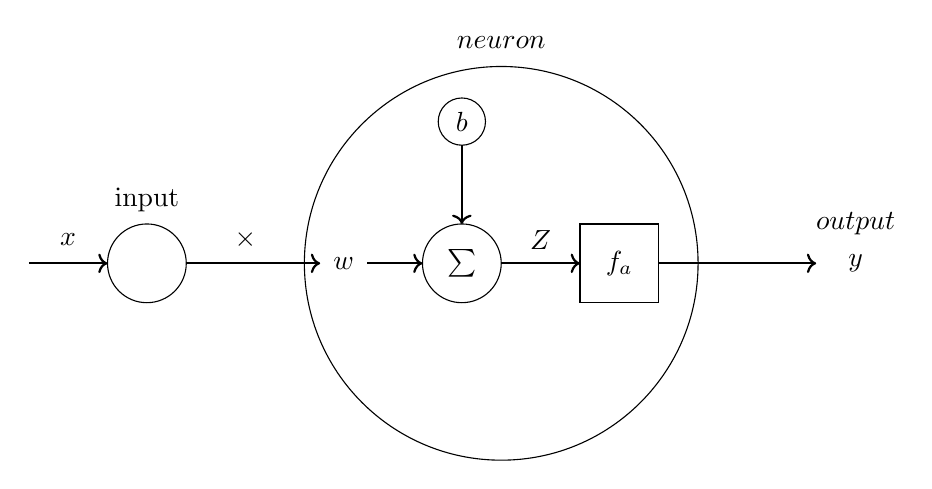
\begin{tikzpicture}
			% Draw the first circle
			\draw[->, thick] (2.5,0) -- (3.5,0);
			\node at (3,0.3) {$x$};
			\draw (4,0) circle (0.5);
			\node at (4,0.8) {input};
			
			% Draw the arrow
			\draw[->, thick] (4.5,0) -- (6.2,0);
			\node at (5.25,0.3) {$\times$};
			\node at (6.5,0) {$w$};
			\draw[->, thick] (6.8,0) -- (7.5,0);
			% Draw the second circle
			\draw (8.5,0) circle (2.5);
			\node at (8.5,2.8) {$neuron$};
			\draw (8,0) circle (0.5);
			\node at (8,0) {$\sum$};
			\draw (8,1.8) circle (0.3);
			\node at (8,1.8) {$b$};
			\draw[->, thick] (8,1.5) -- (8,0.5);
			
			\draw[->, thick] (8.5,0) -- (9.5,0);
			\node at (9,0.3) {$Z$};
			\draw (9.5,-0.5) rectangle(10.5,0.5);
			\node at (10,0) {$f_a$};
			
			\draw[->, thick] (10.5,0) -- (12.5,0);
			\node at (13,0) {$y$};
			\node at (13,0.5) {$output$};
			
		\end{tikzpicture}
		\caption{Single Input - Single Neuron - Single Output}
	\end{figure}
	
	
	We can formulate such a model with:
	
	$$Z = w \cdot x + b$$
	
	$$y = f_a(Z)$$
	
	
	\begin{itemize}
		\item $x$ is the independent variable (input)
		\item $w$ is called \textbf{w}eight for the input, calibrated by training the model
		\item $b$ stand for \textbf{b}ias, calibrated by training
		\item $f_a$ is called \textbf{a}ctivation function given by user when designing the model
	\end{itemize}
	
	Essentially, $y$ is called the output of the model which we want to predict based on the given input $x$. The activation function can be any function but also it can vary depending on the requirements and specific use case. Common activation functions include the sigmoid function, ReLU (Rectified Linear Unit), Tanh, etc. The activation function introduces non-linearity to the model, allowing the neural network to learn complex relationships between the input and output. If we say $f_a(Z) = Z$ then we are not using any activation function ($y = Z$). In this case there is no difference between this ANN model and a simple \href{https://en.wikipedia.org/wiki/Linear_regression}{Linear Regression} with only one independent variable $x$.
	
	
	What if we have multiple inputs to the neuron? In this case we will have a vector of inputs ($x_1, x_2, ..., x_n$) where $n$ shows the number of inputs. For each input we will have one weight ($w_1, w_2, ..., w_n$). Following figure can show this concept:
	
	
	\begin{figure}[h!]
		\centering
		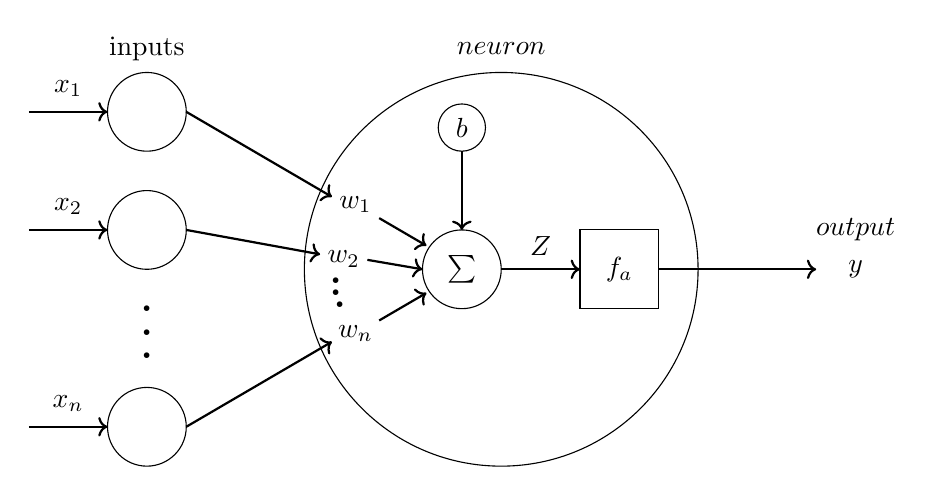
\begin{tikzpicture}
			% Draw the first circle
			\draw[->, thick] (2.5,2) -- (3.5,2);
			\node at (3,2.3) {$x_1$};
			\node at (4,2.8) {inputs};
			\draw (4,2) circle (0.5);
			\draw[->, thick] (4.5,2) -- (6.35,0.92);
			\node at (6.65,0.82) {$w_1$};
			\draw[->, thick] (6.95,0.65) -- (7.55,0.3);
			
			
			\draw[->, thick] (2.5,0.5) -- (3.5,0.5);
			\node at (3,0.8) {$x_2$};
			\draw (4,0.5) circle (0.5);
			\draw[->, thick] (4.5,0.5) -- (6.2,0.19);
			\node at (6.5,0.13) {$w_2$};
			\draw[->, thick] (6.8,0.12) -- (7.5,0);
			
			\node at (4,-0.5) {{\Huge .}};
			\node at (4,-0.8) {{\Huge .}};
			\node at (4,-1.1) {{\Huge .}};
			\node at (6.4,-0.15) {{\Huge .}};
			\node at (6.4,-0.3) {{\Huge .}};
			\node at (6.45,-0.45) {{\Huge .}};
			
			\draw[->, thick] (2.5,-2) -- (3.5,-2);
			\node at (3,-1.7) {$x_n$};
			\draw (4,-2) circle (0.5);
			\draw[->, thick] (4.5,-2) -- (6.35,-0.92);
			\node at (6.65,-0.82) {$w_n$};
			\draw[->, thick] (6.95,-0.650) -- (7.55,-0.3);
			
			% Draw the second circle
			\draw (8.5,0) circle (2.5);
			\node at (8.5,2.8) {$neuron$};
			\draw (8,0) circle (0.5);
			\node at (8,0) {$\sum$};
			\draw (8,1.8) circle (0.3);
			\node at (8,1.8) {$b$};
			\draw[->, thick] (8,1.5) -- (8,0.5);
			
			\draw[->, thick] (8.5,0) -- (9.5,0);
			\node at (9,0.3) {$Z$};
			\draw (9.5,-0.5) rectangle(10.5,0.5);
			\node at (10,0) {$f_a$};
			
			\draw[->, thick] (10.5,0) -- (12.5,0);
			\node at (13,0) {$y$};
			\node at (13,0.5) {$output$};
			
		\end{tikzpicture}
		\caption{Multiple Inputs - Single Neuron - Single Output}
	\end{figure}
	
	
	This problem is similar to a linear regression with multiple independent variable. The neuron processes the input data using its weight\textbf{s} ($w_i$), base ($b$) and activation function ($f_a$) to produce an output.
	
	$$ Z = \sum\limits_{i=1}^{n} w_i \cdot x_i + b = w_1 \cdot x_1 + w_2 \cdot x_2 + ... + w_n \cdot x_n + b$$
	
	$$y = f_a(Z)$$
	
	
	A more complex model is one with multiple neuron in a hidden layer. In this case, since we are still trying to find a single output $y$, we will need an extra output layer, to combine the outputs from all neurons something like the following figure:
	
	\begin{figure}[h!]
		\centering
		
		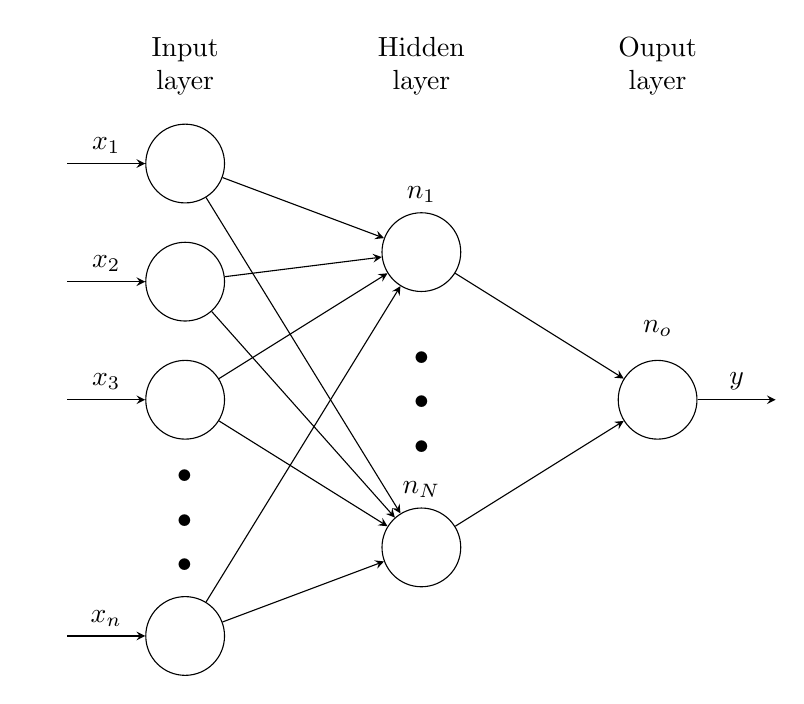
\begin{tikzpicture}[x=1.5cm, y=1.5cm, >=stealth]
			
			\foreach \m/\l [count=\y] in {1,2,3,missing,4}
			\node [every neuron/.try, neuron \m/.try] (input-\m) at (0,2.5-\y) {};
			
			\foreach \m [count=\y] in {1,missing,2}
			\node [every neuron/.try, neuron \m/.try ] (hidden-\m) at (2,2-\y*1.25) {};
			
			\foreach \m [count=\y] in {1} %{1,missing,2}
			\node [every neuron/.try, neuron \m/.try ] (output-\m) at (4,0.5-\y) {}; %(4,1.5-\y)
			\node at (4,.1) {$n_o$}; 
			
			\foreach \l [count=\i] in {1,2,3,n}
			\draw [<-] (input-\i) -- ++(-1,0)
			node [above, midway] {$x_\l$};
			
			\foreach \l [count=\i] in {1,N}
			\node [above] at (hidden-\i.north) {$n_\l$};
			
			\foreach \l [count=\i] in {1} %{1,n}
			\draw [->] (output-\i) -- ++(1,0)
			node [above, midway] {$y$}; %node [above, midway] {$y_\l$};
			
			\foreach \i in {1,...,4}
			\foreach \j in {1,...,2}
			\draw [->] (input-\i) -- (hidden-\j);
			
			\foreach \i in {1,...,2}
			\foreach \j in {1,...,1}
			\draw [->] (hidden-\i) -- (output-\j);
			
			\foreach \l [count=\x from 0] in {Input, Hidden, Ouput}
			\node [align=center, above] at (\x*2,2) {\l \\ layer};
			
		\end{tikzpicture}
		
		\caption{Multiple Inputs - Multiple Neurons - Single Output}
	\end{figure}
	
	
	In this case, \textbf{each} neuron processes the input data using its weight\textbf{s} ($w_{i,j}$), base ($b$) and activation function ($f_a$) to produce an output. The counter $i$ shows how many neurons are in this layer which in this case it starts from $1$ to $N$. The total number of weights for each neuron in the hidden layers equal to the total number of outputs (or the total number of neurons) from previous layer. So, $w_{i,j}$ shows the weights for the $i-th$ neuron in the hidden layer, and the counter $j$ shows how many weights it will have. The previous layer is the input layer ($x_1$, $x_2$, ..., $x_n$) and it has $n$ number of output (in case all neurons are fully connected to the previous layer). So the numbering for weights $j$ \textbf{must} start from $1$ to $n$. Then, for each neuron we will have:
	
	$$Z_{i} = b_{i} + \sum\limits_{j=1}^{j=n} w_{i,j} \times x_{j}$$
	
	$Z_{i}$ is the linear output of each neuron before it goes through an activation function. If we consider all neurons have the same activation function $f_a$, the final output of $i-th$ neuron can be represented by:
	
	$$a_{i} = f_{a}(Z_{i})$$
	
	The neuron $i$th will have a final output of $a_{i}$. $a_{i}$ will be the inputs for the next layer which in this case it is the \textbf{output layer} with a single neuron named $n_o$. The number of weights in this neuron must be equal to the number of outputs in the previous layer which is $N$. So for the \textbf{output layer} we will have:
	
	
	$$Z_{o} = b_{o} + \sum\limits_{j=1}^{j=N} w_{o,j} \times a_{j}$$
	
	$Z_{o}$ is the linear output of neuron $n_o$. If we say this layer is also using the same type of activation function $f_a$, then:
	
	$$y = f_{a}(Z_{o})$$
	
	
	Instead of having only one output ($y$), in some models we might have multiple outputs ($y_1$, $y_2$, ..., $y_K$). The only difference is the \textbf{output layer} must have one neuron for each output:
	
	\begin{figure}[h!]
		\centering
		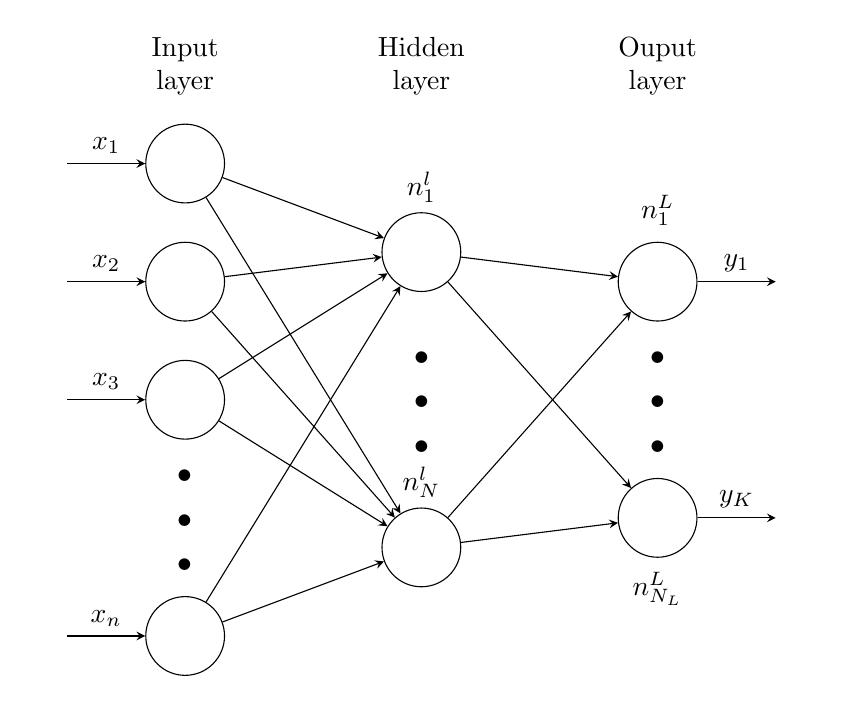
\begin{tikzpicture}[x=1.5cm, y=1.5cm, >=stealth]
			
			\foreach \m/\l [count=\y] in {1,2,3,missing,4}
			\node [every neuron/.try, neuron \m/.try] (input-\m) at (0,2.5-\y) {};
			
			\foreach \m [count=\y] in {1,missing,2}
			\node [every neuron/.try, neuron \m/.try ] (hidden-\m) at (2,2-\y*1.25) {};
			
			\foreach \m [count=\y] in {1,missing,2}
			\node [every neuron/.try, neuron \m/.try ] (output-\m) at (4,1.5-\y) {};
			\node at (4,1.1) {$n^{L}_{1}$};
			\node at (4,-2.1) {$n^{L}_{N_L}$};
			
			\foreach \l [count=\i] in {1,2,3,n}
			\draw [<-] (input-\i) -- ++(-1,0)
			node [above, midway] {$x_\l$};
			
			\foreach \l [count=\i] in {1,N}
			\node [above] at (hidden-\i.north) {$n^{l}_{\l}$};
			
			\foreach \l [count=\i] in {1,K}
			\draw [->] (output-\i) -- ++(1,0)
			node [above, midway] {$y_\l$};
			
			\foreach \i in {1,...,4}
			\foreach \j in {1,...,2}
			\draw [->] (input-\i) -- (hidden-\j);
			
			\foreach \i in {1,...,2}
			\foreach \j in {1,...,2}
			\draw [->] (hidden-\i) -- (output-\j);
			
			\foreach \l [count=\x from 0] in {Input, Hidden, Ouput}
			\node [align=center, above] at (\x*2,2) {\l \\ layer};
			
		\end{tikzpicture}
		\caption{Multiple Inputs - Multiple Neurons - Multiple Outputs}
	\end{figure}
	
	First, since we have two layers (hidden and output) with different number of neurons, the name of neurons are determined by the superscript $l$ in $n^l_{i}$ or $L$ in $n^L_{i}$, for the hidden layer and output layer, respectively. The hidden layer $l$ has $N$, and output layer has $N_L$ number of neurons. 	\textbf{Each} neuron processes the input data using its weight\textbf{s} ($w_{i,j}$), base ($b$) and activation function ($f_a$) to produce an output. The counter $i$ shows how many neurons are in this layer which in this case it starts from $1$ to $N$. The total number of weights for each neuron in the hidden layers equal to the total number of outputs (or the total number of neurons) from previous layer. So, $w_{i,j}$ shows the weights for the $i-th$ neuron in the hidden layer, and the counter $j$ shows how many weights it will have. The layer before hidden layer is the input layer ($x_1$, $x_2$, ..., $x_n$) and it has $n$ number of outputs (in case all neurons are fully connected to the previous layer). So the numbering for weights $j$ \textbf{must} start from $1$ to $n$. Then, for each neuron we will have:
	
	$$Z_{i} = b_{i} + \sum\limits_{j=1}^{j=n} w_{i,j} \times x_{j}$$
	
	$Z_{i}$ is the linear output of each neuron before it goes through an activation function. If we consider all neurons have the same activation function $f_a$, the final output of $i-th$ neuron can be represented by:
	
	$$a_{i} = f_{a}(Z_{i})$$
	
	Each neuron $i$th will have a final output $a_{i}$. So far everything is similar to one output model. Here, $a_{i}$ will be the inputs for the next layer which is the \textbf{output layer} with \textbf{multiple neurons}. The number of weights in each neuron must be equal to the number of outputs in the previous layer which is $N$. So, for the \textbf{output layer} we will have:
	
	
	$$Z_{i} = b_{i} + \sum\limits_{j=1}^{j=N} w_{i,j} \times a_{j}$$
	
	$Z_{i}$ is the linear output of neuron $i$. If we say this layer is also using the same type of activation function $f_a$, then:
	
	$$y_i = f_{a}(Z_{i})$$
	
	
	\subsection{Multilayer Perceptron Forward Pass Formulation}
	
	There are many real world problems that need a more complex ANN with multiple hidden layer, shown in the following figure:
	
	
	\begin{figure}[h!]
		\centering
		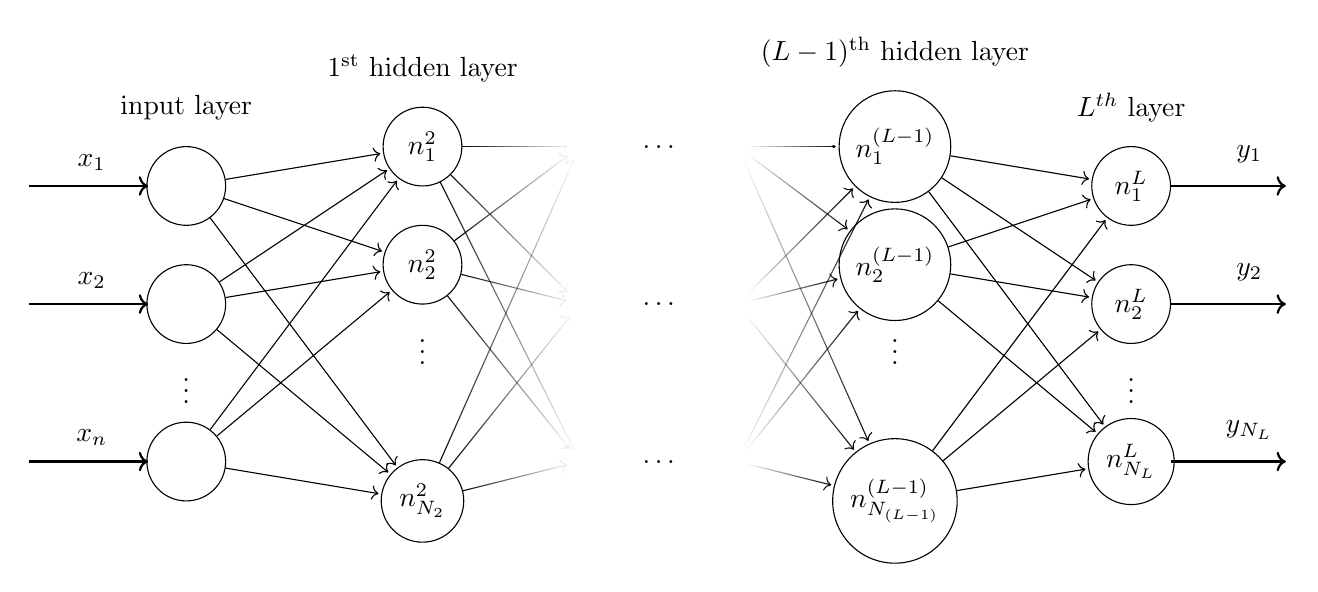
\begin{tikzpicture}[shorten >=1pt]
			\tikzstyle{unit}=[draw,shape=circle,minimum size=1cm]
			%\tikzstyle{hidden}=[draw,shape=circle,fill=black!25,minimum size=1.15cm]
			\tikzstyle{hidden}=[draw,shape=circle,minimum size=1cm]
			
			\node[unit](x0) at (0,3.5){};
			\node at (-1.2,3.8){$x_1$};
			\draw[->, thick] (-2,3.5) -- (-0.45,3.5);
			
			
			\node[unit](x1) at (0,2){};
			\node at (-1.2,2.3){$x_2$};
			\draw[->, thick] (-2,2) -- (-0.45,2);
			
			\node at (0,1){\vdots};
			\node[unit](xd) at (0,0){};
			\node at (-1.2,0.3){$x_n$};
			\draw[->, thick] (-2,0) -- (-0.45,0);
			
			
			
			
			\node[hidden](h10) at (3,4){$n_1^{2}$};
			\node[hidden](h11) at (3,2.5){$n_2^{2}$};
			\node at (3,1.5){\vdots};
			\node[hidden](h1m) at (3,-0.5){$n_{N_2}^{2}$};
			
			\node(h22) at (5,0){};
			\node(h21) at (5,2){};
			\node(h20) at (5,4){};
			
			\node(d3) at (6,0){$\ldots$};
			\node(d2) at (6,2){$\ldots$};
			\node(d1) at (6,4){$\ldots$};
			
			\node(hL12) at (7,0){};
			\node(hL11) at (7,2){};
			\node(hL10) at (7,4){};
			
			\node[hidden](hL0) at (9,4){$n_1^{(L-1)}$};
			\node[hidden](hL1) at (9,2.5){$n_2^{(L-1)}$};
			\node at (9,1.5){\vdots};
			\node[hidden](hLm) at (9,-0.5){$n_{N_{(L-1)}}^{(L-1)}$};
			
			\node[unit](y1) at (12,3.5){$n_1^{L}$};
			\node at (13.5,3.9){$y_1$};
			\draw[->, thick] (12.5,3.5) -- (14,3.5);
			
			\node[unit](y2) at (12,2){$n_2^{L}$};
			\node at (13.5,2.4){$y_2$};
			\draw[->, thick] (12.5,2) -- (14,2);
			
			
			\node at (12,1){\vdots};	
			\node[unit](yc) at (12,0){$n_{N_L}^{L}$};
			\node at (13.5,0.4){$y_{N_L}$};
			\draw[->, thick] (12.5,0) -- (14,0);
			
			
			\draw[->] (x0) -- (h10);
			\draw[->] (x0) -- (h11);
			\draw[->] (x0) -- (h1m);
			
			\draw[->] (x1) -- (h10);
			\draw[->] (x1) -- (h11);
			\draw[->] (x1) -- (h1m);
			
			\draw[->] (xd) -- (h10);
			\draw[->] (xd) -- (h11);
			\draw[->] (xd) -- (h1m);
			
			\draw[->] (hL0) -- (y1);
			\draw[->] (hL0) -- (yc);
			\draw[->] (hL0) -- (y2);
			
			\draw[->] (hL1) -- (y1);
			\draw[->] (hL1) -- (yc);
			\draw[->] (hL1) -- (y2);
			
			\draw[->] (hLm) -- (y1);
			\draw[->] (hLm) -- (y2);
			\draw[->] (hLm) -- (yc);
			
			\draw[->,path fading=east] (h10) -- (h20);
			\draw[->,path fading=east] (h10) -- (h21);
			\draw[->,path fading=east] (h10) -- (h22);
			
			\draw[->,path fading=east] (h11) -- (h20);
			\draw[->,path fading=east] (h11) -- (h21);
			\draw[->,path fading=east] (h11) -- (h22);
			
			\draw[->,path fading=east] (h1m) -- (h20);
			\draw[->,path fading=east] (h1m) -- (h21);
			\draw[->,path fading=east] (h1m) -- (h22);
			
			\draw[->,path fading=west] (hL10) -- (hL0);
			\draw[->,path fading=west] (hL11) -- (hL0);
			\draw[->,path fading=west] (hL12) -- (hL0);
			
			\draw[->,path fading=west] (hL10) -- (hL1);
			\draw[->,path fading=west] (hL11) -- (hL1);
			\draw[->,path fading=west] (hL12) -- (hL1);
			
			\draw[->,path fading=west] (hL10) -- (hLm);
			\draw[->,path fading=west] (hL11) -- (hLm);
			\draw[->,path fading=west] (hL12) -- (hLm);
			
			\node at (0,4.5) {input layer};
			\node at (3,5) {$1^{\text{st}}$ hidden layer};
			\node at (9,5.2) {$(L-1)^{\text{th}}$ hidden layer};
			\node at (12,4.5) {$L^{th}$ layer};
		\end{tikzpicture}
		\caption{{\footnotesize Network Network of a $(L)$-layer perceptron with $n$ input units and $N_L$ outputs. Layer $l^{th}$ has $N_l$ number of neurons. Every neuron in $l^{th}$ layer  ($n^l_i$) will have a bias $b_{i}^{l}$.}}
		\label{fig:multilayer-perceptron}
	\end{figure}
	
	
	
	
	The above figure shows a model in which can have multiple hidden layer and each hidden layer can have different number of neurons. Let:
	
	\begin{itemize}
		\item $X_j$ be the input of the neural network with $j=1:n$ where $n$ is the total number of inputs to the model.
		
		\item $L$ be the total number of layers (including input and output layers),
		
		\item $N_l$ is the total number of neuron is in the layer $l$
		
		\item $w_{i,j}^{l}$ be the weights in layer $l$, and $i=1:N_l$ is defining the weights for neuron $i-th$ in this layer, and $j=1:N_{l-1}$ is the number of weight that each neuron \textbf{must} have. \textbf{The total number of weights for each neuron in layer $l$ is equal to the total number of outputs (or the total number of neurons) from previous layer $l-1$.}
		
		\item $b_{i}^{l}$ be the bias for neuron $i-th$ in layer $l$, 
		
		\item $Z_{i}^{l}$ the output of neuron $i-th$ in layer $l$
		
		\item in $f_{a,i}^{l}(Z_{i}^{l})$, the $f_{a,i}^{l}$ is the activation function applied to the linear output of neuron $i-th$ in layer $l$,
		
		\item and in $a_{i}^{l}=f_{a,i}^{l}$, the $a_{i}^{l}$ be the final output from neuron $i-th$ in the layer $l$.
	\end{itemize}
	
	$l=1$ represent the input layer to the model. Since in this layer NN doesn't have any weights and activation functions, we can say that the final output of the first layer (\textbf{input layer}) $a_{j}^{l=1}$ is:
	
	$$a_{j}^{1}= X_j$$
	
	From the second layer $l=2$ (\textbf{first hidden layer}) to the \textbf{last (output) layer} $L$:
	
	$$Z_{i}^{l} = b_{i}^{l} + \sum\limits_{j=1}^{N_{l-1}} w_{i,j}^{l} \times a_{j}^{l-1}$$
	
	The output of each neuron must go through the corresponding activation function:
	
	$$a_{i}^{l} = f_{a,i}^{l}(Z_{i}^{l})$$
	
	\noindent where $a_{i}^{l}$ is final output of the layer $l$ and the input values of next layer $l+1$. When the ANN model has multiple outputs ($y_1, y_2, ..., y_{N_L}$) (multiple neurons in the output layer), then for each neuron, the model will have one output $a_{i}^{L}$:
	
	$$Z_{i}^{L} = b_{i}^{L} + \sum\limits_{j=1}^{N_{L-1}} w_{i,j}^{L} \times a_{j}^{L-1}$$
	
	$$y_i = a_{i}^{L} = f_{a,i}^{L}(Z_{i}^{L})$$
	
	
	For instance, if the ANN model has one output ($y$) (one neuron in the output layer), then:
	
	$$Z_{1}^{L} = b_{1}^{L} + \sum\limits_{j=1}^{N_{L-1}} w_{1,j}^{L} \times a_{j}^{L-1}$$
	
	$$y = a_{1}^{L} = f_{a,1}^{L}(Z_{1}^{L})$$
	
	
	
	
	\subsubsection*{A Numerical Example for Multilayer Perceptron Formulation}
	
	Consider a dataset with 4 inputs (independent variables $x_1, x_2, x_3, x_4$) and one output (dependent variable $y$). The target is to create a model which is able to predict the output with a set of given inputs. In another word, we are creating a function $y = f(x_1, x_2, x_3, x_4)$. These are the information we obtain by looking at the physics and the nature of the problem. For instance, you are asked to create a model predicting the blood pressure $y$ of patients in $[mm Hg]$ unit, based on Lopressor dosage per day $[mg/day]$ as $(x_1)$, body weight in $[kg]$ as $(x_2)$, age in $[year]$ as $(x_3)$, and hours playing online video games like Dota 2 in $[hours/day]$ as $(x_4)$. Necessarily all the factors are not going to have the same effects on blood pressure. For example, it is said (\textbf{this not my area of expertise}) \href{https://www.accessdata.fda.gov/drugsatfda_docs/label/2013/018704s026lbl.pdf}{Lopressor} is a medication to lower the blood pressure, but playing Dota 2 increases my blood pressure!
	
	
	Having all above information, we can decide about the architecture of input and output layers in ANN model. This means the input layer must have 4 neurons and the last layer will have one neuron. Since the output layer has a continues floating point value, we can also say the output layer can have linear activation function. About the architecture of hidden layers, we can decide only when we actually start training the model. We usually start with simple models and if necessary we increase the complexity of architecture by increasing the number of hidden layers and neurons in each hidden layer. However, there is a limit for that and it's called \textbf{overfitting}. At this moment let's just consider a simple model which the formulation is easier to explain:	
	
	\begin{itemize}
		\item If the number of inputs are 4 then $n=4$.
		
		\item We \textbf{assume} there is only 2 hidden layer is needed, which referred by $l=2$ and $l=3$. So the total of number of layers is equal to 4 ($L=4$).
		
		\item We \textbf{assume}, two neurons is the first hidden layer is enough. This means the number of neurons in the layer $l=2$ is $N_2=2$ referred by $n^2_1$ and $n^2_2$ names. Since the previous layer $l=2-1$ had 4 outputs, every neuron in this layer \textbf{must} have 4 weights ($w_{i,j}^2$), where $j=1:4$ is the numbering for weights and $i=1:2$ shows the number of neurons in the layer $l=2$. So, this layer will have 2 outputs ($a_{1}^{2}$ and $a_{2}^{2}$).
		
		\item We \textbf{assume} the number of neurons in the layer $l=3$ is 4 ($N_3=4$) with $n^3_1$, $n^3_2$, $n^3_3$ and $n^3_4$ names. Since the previous layer $l=3-1$ had 2 outputs, every neuron in this layer \textbf{must} have 2 weights ($w_{i,j}^3$), where $j=1:2$ is the numbering for weights and $i=1:4$ shows the number of neurons in the layer $l=3$. So, this layer will have 4 outputs ($a_{1}^{3}$, $a_{2}^{3}$, $a_{3}^{3}$, $a_{4}^{3}$).
		
		\item Only one output ($y$), then output layer will have one neuron ($n^L_1$). Since the previous layer $l=4-1$ had 4 outputs, the only neuron in this layer \textbf{must} have 4 weights ($w_{i=1,j}^4$), where $j=1:4$ is the numbering for weights and $i=1$ shows the only neurons in the output layer $l=L=4$. So, this layer will have 1 output ($y = a_{1}^{4}$)
	\end{itemize}
	
	This is how the ANN model looks like:
	% Input layer neurons'number
	\newcommand{\inputnum}{4} 
	
	% Output layer neurons'number
	\newcommand{\outputnum}{1} 
	
	
	\begin{figure}[h!]
		\begin{center}
			\begin{tikzpicture}
				
				% Input Layer
				\foreach \i in {1,...,\inputnum}
				{
					\node[circle, 
					minimum size = 6mm,
					fill=orange!90!black] (Input-\i) at (0,-\i) {};
				}
				
				% Hidden Layer
				\foreach \i in {1,2}
				{
					\node[circle, 
					minimum size = 6mm,
					fill=teal!50,
					yshift=(2-\inputnum)*5 mm
					] (Hidden1-\i) at (2.5,-\i) {};
				}
				
				% Hidden Layer
				\foreach \i in {1,2,3,4}
				{
					\node[circle, 
					minimum size = 6mm,
					fill=teal!50,
					yshift=(4-\inputnum)*5 mm
					] (Hidden2-\i) at (5,-\i) {};
				}
				
				% Output Layer
				\foreach \i in {1}
				{
					\node[circle, 
					minimum size = 6mm,
					fill=purple!50,
					yshift=(\outputnum-\inputnum)*5 mm
					] (Output-\i) at (7.5,-\i) {};
				}
				
				% Connect neurons In-Hidden
				\foreach \i in {1,...,\inputnum}
				{
					\foreach \j in {1,2}
					{
						\draw[->, shorten >=1pt] (Input-\i) -- (Hidden1-\j);   
					}
				}
				
				% Connect neurons Hidden1-Hidden2
				\foreach \i in {1,2}
				{
					\foreach \j in {1,...,4}
					{
						\draw[->, shorten >=1pt] (Hidden1-\i) -- (Hidden2-\j);
					}
				}
				
				% Connect neurons Hidden2-Out
				\foreach \i in {1,...,4}
				{
					\foreach \j in {1,...,\outputnum}
					{
						\draw[->, shorten >=1pt] (Hidden2-\i) -- (Output-\j);
					}
				}
				
				% Inputs
				\foreach \i in {1,...,\inputnum}
				{            
					\draw[<-, shorten <=1pt] (Input-\i) -- ++(-1,0)
					node[left]{$x_{\i}$};
				}
				
				% Outputs
				\foreach \i in {1,...,\outputnum}
				{            
					\draw[->, shorten <=1pt] (Output-\i) -- ++(1,0)
					node[right]{$y$};
				}
				
			\end{tikzpicture}
		\end{center}
		\caption{{\footnotesize The orange color circles show the inputs layer, green ones shows two hidden layers, and the purple circle is the output layer with one neuron.}}
	\end{figure}
	
	
	
	
	For \textbf{l=2}, the linear output from each neuron $n^2_1$ and $n^2_2$ are:
	
	$$Z_{1}^{2} = w_{1,1}^{2} \cdot X_1     + w_{1,2}^{2} \cdot X_2     + w_{1,3}^{2} \cdot X_3     +w_{2,4}^{2} \cdot X_4      + b_{1}^{2}$$
	
	$$Z_{2}^{2} = w_{2,1}^{2} \cdot X_1      +      w_{2,2}^{2} \cdot X_2     +        w_{2,3}^{2} \cdot X_3          +           w_{2,4}^{2} \cdot X_4 + b_{2}^{2}$$
	
	
	The linear output goes through an activation function $f_{a,i}^{2}()$ which each neuron can have a different activation function, but to simplify the formulation lets say $f_{a}^{2}()$ which means the whole layer will have the same activation function
	so the final outputs of $l=2$ layer or the inputs of the next layer ($l=3$) will be:
	
	$$a_{1}^{2} = f_{a}^{2}(Z_{1}^{2})$$
	$$a_{2}^{2} = f_{a}^{2}(Z_{2}^{2})$$
	
	\textbf{In the next layer ($l=3$)}, which is the last hidden layer, the model has 4 neurons each with 2 weights (the number of outputs in the previous layer):
	
	$$Z_{1}^{3} = w_{1,1}^{3}    \cdot     a_{1}^{2}        +      w_{1,2}^{3}    \cdot      a_{2}^{2}      + b_{1}^{3}$$
	
	$$Z_{2}^{3} = w_{2,1}^{3}    \cdot     a_{1}^{2}        +      w_{2,2}^{3}    \cdot      a_{2}^{2}      + b_{2}^{3}$$
	
	$$Z_{3}^{3} = w_{3,1}^{3}    \cdot     a_{1}^{2}        +      w_{3,2}^{3}    \cdot      a_{2}^{2}      + b_{3}^{3}$$
	
	$$Z_{4}^{3} = w_{4,1}^{3}    \cdot     a_{1}^{2}        +      w_{4,2}^{3}    \cdot      a_{2}^{2}      + b_{4}^{3}$$
	
	So, final outputs of layer $l=3$ will be:
	
	$$a_{1}^{3} = f_{a}^{3}(Z_{1}^{3})$$
	$$a_{2}^{3} = f_{a}^{3}(Z_{2}^{3})$$
	$$a_{3}^{3} = f_{a}^{3}(Z_{3}^{3})$$
	$$a_{4}^{3} = f_{a}^{3}(Z_{4}^{3})$$
	
	
	
	
	\textbf{The next layer which is the last layer ($l=L$)} will have 4 inputs including $a_{1}^{3}$, $a_{2}^{3}$,  $a_{3}^{3}$, $a_{4}^{3}$, meaning every neuron must have 4 weights. With single neuron (single output) in this layer, we have:
	
	$$Z_{1}^{4} = w_{1,1}^{4}\cdot a_{1}^{3}    + w_{1,2}^{4}\cdot a_{2}^{3}    + w_{1,3}^{4}\cdot a_{3}^{3}     +w_{2,4}^{4}\cdot  a_{4}^{3}      + b_{1}^{4}$$
	
	\noindent and the final output will be:
	$$y = a_{1}^{4} = f_{a}^{4}(Z_{1}^{4})$$
	
	
	
	
	
	
	
	
	
	
	
	\subsubsection*{Activation Function}
	
	Let's talk about $f_a$ known as activation function. The choice of activation function depends on the nature of the output variable $y$ and the specific requirements of the problem. Here are the typical activation functions for the three possible scenarios:
	
	\textcolor{orange!80!black}{- Binary Classification (Binary Output):}
	
	
	Let's say we want to categorize a photo say if it is a picture of a "dog". In this case, the ANN model is called \textbf{Binary Classification}. There is only two categories and ANN must determine which one it is! The output is "Yes" or "No". It is "True" or "False", or it is "1" or "0". These types of problem's can be modelled by only one output $y$. For example, we use the activation function like \textbf{Sigmoid} function:
	
	$$y = f_{a}(Z) = \dfrac{1}{1 + e^{-Z}}$$
	
	
	
	The Sigmoid function squashes the output to a value between 0 and 1, which can be interpreted as the probability of the input belonging to the positive class (class 1). For instance:
	
	
	\begin{itemize}
		
		\item If $Z \in (-\inf, 0)$, then $y \in [0,\ 0.5)$ and we can assign this range of $y$ to class 1.
		
		\item If $Z \in (0 +\inf)$, then $y \in (0.5,\ 1]$, which will be class 2.
		
	\end{itemize}
	
	\begin{figure}[h!]
		\centering
		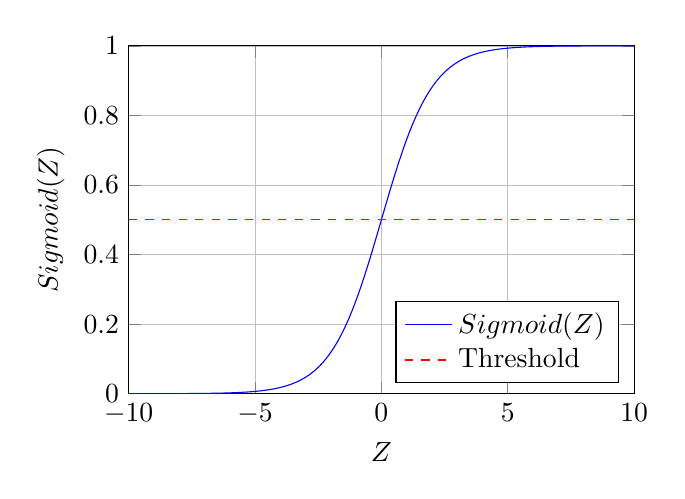
\begin{tikzpicture}
			\begin{axis}[
				xlabel=$Z$,
				ylabel=$Sigmoid(Z)$,
				ymin=0, ymax=1,
				xmin=-10, xmax=10,
				width=8cm, height=6cm,
				grid=both,
				grid style={line width=0.1pt, draw=gray!30},
				major grid style={line width=0.2pt, draw=gray!50},
				legend pos=south east,
				legend cell align=left,
				]
				\addplot[domain=-10:10, samples=100, smooth, blue] {1/(1 + exp(-x))};
				\legend{$Sigmoid(Z)$}
				
				% Adding the threshold line
				\addplot[domain=-10:10, red, dashed] {0.5};
				\addlegendentry{Threshold}
			\end{axis}
		\end{tikzpicture}
		\caption{{\footnotesize Sigmoid function plot with \textbf{a} threshold line.}}
		\label{fig:sigmoid_plot}
	\end{figure}
	
	
	\textcolor{orange!80!black}{- Multi-Class Classification (Probabilities for Each Class):}
	
	Sometimes we might have multiple outputs ($y_1$, $y_2$, ..., $y_K$). For example, if ANN model is responsible to determine the category between "dog", "cat", and "horse". In this case, we need to have \textbf{three} outputs ($y_1$, $y_2$, $y_3$), and each output must give us the probability of each category. For example, for a specific set of inputs ($x_i$), the outputs of the model are $y_1 = 0.25$, $y_2 = 0.65$, and $y_3 = 0.10$, then we can say the chances that this photo is showing a "cat" or $y_2$ is $65\%$.
	
	These types of problems are called \textbf{Multi-Class Classification} (Probabilities for Each Class). In multi-class classification, each output $y$ represents the probability of the input belonging to a particular class. The most common activation function for the output layer in this case is the \textbf{Softmax} function. The Softmax function ensures that the probabilities for all classes sum up to 1. It provides a probability distribution over the different classes. The formula for the Softmax activation function is:
	
	$$y_i = f_{a}(Z_i) = \dfrac{e^{Z_i}}{\sum\limits_{j=1}^{N_L} e^{Z_j}}$$
	
	\noindent where $Z_i$ is the output for class $i$, $N_L$ the number of classes or outputs (or the number of neurons in the output layer), and $y_i = f_{a}(Z_i)$ represents the probability of the inputs belonging to class $i$ which it will be a number between 0 to 1. Since we are talking about probability, $\sum_{i=1}^{N_L} y_i = 1$, meaning the summation of all chances must be equal to 100\%.
	
	\textcolor{orange!80!black}{- Regression (Continuous Real-Valued Output):}
	
	In regression problems where the output $y$ is a continuous real value, the most commonly used activation function for the output layer is the \textbf{Linear activation function}. The Linear activation function \textbf{simply outputs the weighted sum of the input features without any non-linearity}. This is the same as the example we had to predict the blood pressure. It allows the neural network to predict continuous values over a wide range. The formula for the Linear activation function  if there is single output is:
	
	$$y = f_a(Z) = Z$$
	
	\noindent which means $Z$ itself is the output and no activation function is applied. Just a reminder, the final output ($y_i$) from each neuron ($i$) in the \textbf{output layer} is $Z_i$. If there are multiple outputs then:
	
	$$y_i = f_{a}(Z_i) = Z_i$$
	
	\begin{figure}[h!]
		\centering
		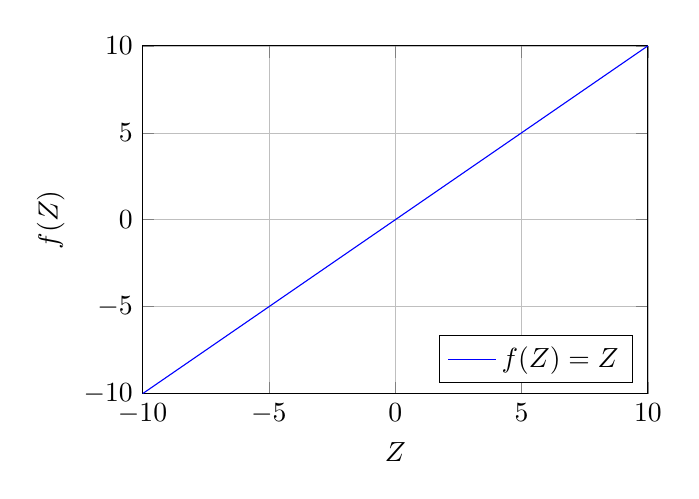
\begin{tikzpicture}
			\begin{axis}[
				xlabel=$Z$,
				ylabel=$f(Z)$,
				ymin=-10, ymax=10,
				xmin=-10, xmax=10,
				width=8cm, height=6cm,
				grid=both,
				grid style={line width=0.1pt, draw=gray!30},
				major grid style={line width=0.2pt, draw=gray!50},
				legend pos=south east,
				legend cell align=left,
				]
				% Linear function: f(Z) = mZ + b
				\addplot[domain=-10:10, samples=100, smooth, blue] {x}; % f(Z) = Z
				\legend{$f(Z) = Z$}
			\end{axis}
		\end{tikzpicture}
		\caption{{\footnotesize Linear function plot with \textbf{a} threshold line.}}
		\label{fig:linear_plot}
	\end{figure}
	
	These activation functions are widely used in their respective scenarios and can be combined with various hidden layer activation functions such as ReLU, Tanh, etc., to build effective neural network architectures for different types of problems.
	
	
	
	
	
	\subsection{Model Training and Backpropagation Formulation}
	
	How we find weights and biases for each neuron in layers? Let's have a real-world example of \textbf{learning not to touch a hot surface}. When we were kids, we likely touched a hot kettle or surface out of curiosity. Here’s how the neural network-like process worked in our brains:
	
	
	\textbf{Inputs (Stimuli)}: The sensory neurons in our skin detected the high temperature of the kettle. This is analogous to inputs in a neural network. These inputs could include:
	
	\begin{itemize}
		\item \textbf{Temperature}: The skin senses an unusually high temperature.
		\item \textbf{Pressure}: The hand presses against the surface.
	\end{itemize}
	
	
	\textbf{Error Signal (Pain):} When the brain registered the pain, this was an "error signal." The brain compared the comfortable state (expected output) with the burning pain (actual output). The error here is the mismatch between the desired state (comfort) and the observed outcome (pain).
	
	
	\textbf{Learning (Adjusting Weights and Biases):} Repeated exposure to similar situations (hot objects) caused the brain to adapt. The pathways in neural network deciding either we should or shouldn't touch something were strengthened to associate high temperatures with pain and avoidance. Over time, the child learned to withdraw their hand instinctively before experiencing pain. This is the output of the neural network: a correct prediction or decision to avoid hot surfaces. The brain also generalized this learning. Even without touching other hot surfaces (e.g., a stovetop or boiling water), the child would instinctively avoid them. In neural networks, this is analogous to generalization—applying learned patterns to unseen inputs.
	
	
	The process of calibrating or optimizing the weights and biases in an Artificial Neural Network (ANN) is typically done through a process called "training" or "learning" by \textbf{forward} and \textbf{backward} \textbf{propagation} functions. The goal of training is to adjust the parameters (weights and biases) of the network so that it can make accurate predictions on the given data. The most common approach to training an ANN is using an optimization algorithm called \textbf{Stochastic Gradient Descent} (SGD) or its variants, e.g Adam. Adam (Adaptive Moment Estimation) is considered a variant of Stochastic Gradient Descent (SGD). While Adam introduces additional mechanisms such as momentum and adaptive learning rates, its core idea still revolves around using gradient-based updates to minimize a loss function. Here's an overview of how the training process works:
	
	\begin{enumerate}
		\item \textbf{Initialization}: The weights and biases in the neural network are initialized with small random values. It's crucial to start with random values to break any symmetry in the network.
		
		\item \textbf{Forward Propagation}: During each training iteration (also known as an epoch), the input data is fed into the network, and the activations for each layer are calculated through forward propagation. The forward pass involves computing the weighted sum of inputs, applying the activation function, and passing it to the next layer.
		
		\item \textbf{Loss Function}: A loss function is defined to quantify how far off the predictions are from the actual targets. The goal of training is to minimize this loss function.
		
		\item \textbf{Backpropagation}: After the forward pass, the error (the difference between the predicted output and the actual target) is calculated using the chosen loss function. Backpropagation is then used to propagate this error backward through the network to update the weights and biases.
		
		\item \textbf{Gradient Calculation}: In backpropagation, the gradients of the loss function with respect to each weight and bias are computed. These gradients indicate the direction and magnitude of adjustments needed to minimize the loss.
		
		\item \textbf{Weight and Bias Update}: The gradients calculated in the previous step are used to update the weights and biases. The learning rate is a hyperparameter that determines the step size taken in the direction of the gradients. Smaller learning rates make smaller updates, while larger learning rates make larger updates. A typical learning rate value might be 0.001 or 0.01, but this can vary depending on the problem and network architecture.
		
		\item \textbf{Repeat}: Steps 2 to 6 are repeated for multiple epochs or until the loss converges to a satisfactory value.
	\end{enumerate}
	
	The training process continues until the neural network parameters reach a state where the loss is minimized, and the model makes accurate predictions on unseen data.
	
	Let's start the formulation of Stochastic Gradient Descent (SGD) to update the weights and bias in training process. Let \( L \) be the total number of layers in the neural network, and \( a_{i}^{L} \) be the output of neuron \( i \) in the output layer. The error for neuron \( i \) in the output layer is given by:
	
	\[
	\delta_{i}^{L} = (a_{i}^{L} - y_{i}) \cdot f_{a, i}^{L'}(Z_{i}^{L})
	\]
	
	\noindent where
	
	\begin{itemize}
		\item \( y_{i} \) is the target output.
		\item \( a_{i}^{L} \) is the predicted output.
		\item \( f_{a, i}^{L'}(Z_{i}^{L}) \) is the derivative of the activation function for neuron \( i \).
		\item \(
		Z_{i}^{L} = b_{i}^{L} + \sum_{j=1}^{N_{L-1}} w_{i,j}^{L} \cdot a_{j}^{L-1}
		\) is the linear output of the last layer.
	\end{itemize}
	
	
	
	
	For any hidden layer \( l \) (where \( l = L-1, L-2, \ldots, 1 \)), the error for neuron \( i \) in layer \( l \) is calculated by propagating the error backward from the next layer \( l+1 \):
	
	\[
	\delta_{i}^{l} = f_{a, i}^{l'}(Z_{i}^{l}) \cdot \sum_{k=1}^{N_{l+1}} w_{k, i}^{l+1} \cdot \delta_{k}^{l+1}
	\]
	
	\noindent where
	\[
	Z_{i}^{l} = b_{i}^{l} + \sum_{j=1}^{N_{l-1}} w_{i,j}^{l} \cdot a_{j}^{l-1}
	\]
	
	For each layer \( l = 1, 2, \ldots, L \), the weights and biases are updated using the following rules:
	
	\begin{itemize}
		\item \( \eta \) is the learning rate.
		\item \( a_{j}^{l-1} \) is the output from the previous layer.
		\item \( \delta_{i}^{l} \) is the error for the current layer.
	\end{itemize}
	
	\noindent Essentially the weights are updated by:
	\[
	w_{i,j}^{l} \leftarrow w_{i,j}^{l} - \eta \cdot \delta_{i}^{l} \cdot a_{j}^{l-1}
	\]
	
	\noindent and the bias can also be updated using:
	\[
	b_{i}^{l} \leftarrow b_{i}^{l} - \eta \cdot \delta_{i}^{l}
	\]
	
	
	
	Here is a \textbf{summary} of propagation algorithm:
	
	\begin{enumerate}
		\item \textbf{Forward Pass:} Compute the activations \( a_{i}^{l} \) for all layers.
		\item \textbf{Compute Output Layer Error:} Compute \( \delta_{i}^{L} \).
		\item \textbf{Backward Pass:} Compute \( \delta_{i}^{l} \) for each hidden layer \( l \) in reverse order.
		\item \textbf{Update Parameters:} Adjust weights \( w_{i,j}^{l} \) and biases \( b_{i}^{l} \) using the calculated errors.
	\end{enumerate}
	
	
	This formulation ensures efficient training of the neural network by adjusting weights and biases to minimize the overall loss.
	
	\subsubsection*{A Numerical Example for Training Model}
	
	
	You must design your ANN model based on the given data. Take the dataset shown in following table as an example. Based on the given data it seems the output $y$, is either 0 or 1 (binary classification problem). So the output layer must have only one neuron, and an activation function that gives us a binary output. So, I can use Sigmoid ($y = f_{a}(Z) = \dfrac{1}{1 + e^{-Z}}$) as activation function for the output layer.
	
	\begin{table}[h!]
		\centering
		\begin{tabular}{|c|c|c|c|}
			\hline
			sample & $x_1$ & $x_2$ & $y$ \\
			\hline
			1 & 0.2 & 0.8 & 1 \\
			2 & 0.7 & 0.4 & 0 \\
			\vdots   & \vdots & \vdots & \vdots \\
			m & 0.1 & 0.1 & 1 \\
			\hline
		\end{tabular}
		\label{tab:my_table}
	\end{table}
	
	As a reminder, this function returns values between 0 and 1. We assume a threshold of $sigmoid (Z) = 0.5$. Any number above this is rounded up to 1 ($y=1$), and lower than this line is considered zero ($y=0$).
	
	The dataset shows two inputs ($x_1$ and $x_2$). \textbf{How many layers between input and output we need?} There is no absolute correct answer to this question, and you have to start with lower number of layers, and increase them gradually to get the right accuracy you are looking for while avoiding \textbf{over-fitting}. In this case, we want a simple example and we don't consider any hidden layer. The following ANN model has one neuron in the output layer (one $y$ output) creating a linear combination of inputs ($x_1$ and $x_2$):
	
	\begin{figure} [h!]
		\begin{center}
			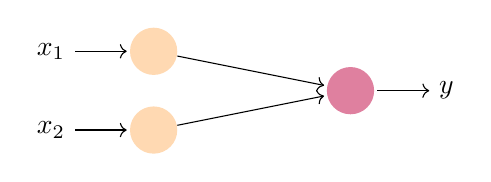
\begin{tikzpicture}
				% Input Layer
				\foreach \i in {1,2}
				{
					\node[circle, 
					minimum size = 6mm,
					fill=orange!30] (Input-\i) at (0,-\i) {};
				}
				% Output Layer
				\foreach \i in {1}
				{
					\node[circle, 
					minimum size = 6mm,
					fill=purple!50,
					yshift=(1-2)*5 mm
					] (Output-\i) at (2.5,-\i) {};
				}
				% Connect neurons In-Hidden
				\foreach \i in {1,...,2}
				{
					\foreach \j in {1}
					{
						\draw[->, shorten >=1pt] (Input-\i) -- (Output-\j);   
					}
				}	
				% Inputs
				\foreach \i in {1,2}
				{            
					\draw[<-, shorten <=1pt] (Input-\i) -- ++(-1,0)
					node[left]{$x_{\i}$};
				}
				% Outputs
				\foreach \i in {1}
				{            
					\draw[->, shorten <=1pt] (Output-\i) -- ++(1,0)
					node[right]{$y$};
				}
			\end{tikzpicture}
		\end{center}
		\caption{{\footnotesize An ANN with two inputs, no hidden layer, and one output.}}
	\end{figure}
	
	After designing the model architecture::
	
	\begin{enumerate}
		\item \textbf{Randomly initialize} the weight and bias for the output layer. Since we have two inputs to the neuron, this neuron must have two weights. Let's say here is the randomized values for weights and bias:
		
		$$
		\begin{bmatrix}
			w_1 & w_2
		\end{bmatrix} = 
		\begin{bmatrix}
			0.3 & 0.5
		\end{bmatrix}
		$$
		
		$$
		\begin{bmatrix}
			b
		\end{bmatrix} = 
		\begin{bmatrix}
			0.1
		\end{bmatrix}
		$$
		
		\item \textbf{Formulation}:
		
		$$Z = w_1 \cdot x_1 + w_2 \cdot x_2 + b_1$$
		
		$$y = Sigmoid(Z)$$
		
		\item \textbf{Training Loop} (for the first two epochs): For simplicity, we'll assume the following training data for only one sample (bach size $= 1$):
		
		
		\textbf{Epoch 1}: Using \textbf{Sample 1} data in the table:
		\begin{itemize}
			\item Forward Propagation:
			
			$$Z = 
			\begin{bmatrix}
				w_1 & w_2
			\end{bmatrix} \times \begin{bmatrix}
				x_1 \\ x_2
			\end{bmatrix}
			+ b = 
			\begin{bmatrix}
				0.3 & 0.5
			\end{bmatrix} \times \begin{bmatrix}
				0.2 \\ 0.8
			\end{bmatrix} + 0.1 = 0.56
			$$
			
			$$y_{preidcted} = Sigmoid(0.56) = 0.63$$
			
			\item Compute the error (loss) for the output layer: The actual output of Sample 1 is $y_{real} = 1$. This is the type of error function I chose. Based on the problem's characteristic, a different loss function (error) might work better! 
			
			$$error = y_{real} - y_{preidcted} = 0.36354745971843361$$
			
			\item Backpropagation and Weight Update: If \( \eta = 0.5 \) is the learning rate, and $\delta w_i$ and $\delta b$ is the amount of changes on weights and bias:
			
			$$w_{1} \xleftarrow{} w_1 + \delta w_1$$
			$$\delta w_1= \eta \cdot y' \cdot error \cdot x_1$$
			
			where $y'$ is the derivative of $y = Sigmoid(Z)$ based on Z, So:
			
			$$Sigmoid'(Z) = Sigmoid(Z) \cdot (Sigmoid(Z) - 1)$$
			
			or in this case we can say:
			
			$$y' = y(y-1)$$
			
			Essentially, we can update $w_2$ and $b$:
			
			$$w_{2} \xleftarrow{} w_2 + \eta \cdot y_{preidcted} \cdot (1-y_{preidcted}) \cdot error \cdot x_2$$
			
			$$b \xleftarrow{} b + \eta \cdot y_{preidcted} \cdot (1-y_{preidcted}) \cdot error$$
			
			The updated values are:
			
			$w_1= 0.3084117867258207$
			
			$w_2= 0.53364714690328274$
			
			$b= 0.14205893362910343$
			
			With the updated values, the error will drop to $0.0.3473611246515993$. Let's say we have a 1000 data samples, and we divide them into 10 groups each with 100 samples (bach size $=1$). We can update the values using this 100 samples before we go to the next epoch!
			
		\end{itemize}
		
		
		\textbf{Epoch 2 to end}: In the previous epoch we used only \textbf{sample 1}. In this, epoch we want to use the second sample (or second bach size). In this case, the error value might drop or increase. But the point of ANN is to keep training over all the available data, until it reaches to the best optimized values. This is the reason why we need a lot of samples when we are training the data. If the model still was not able to decrease the error, one way is to increase the number of hidden layers and neurons to improve the ability of the model to learn more! A larger ANN model means more parameters are needed to be estimated, so we need more samples.
	\end{enumerate}
	
	
	Here is the C code for the mentioned procedure. Be careful, this is not a geneal format for a ANN. This is just a code for the above mentioned example. Use GDB or LLDB debugger to print the intermediate results.
	
	\begin{lstlisting}
		#define INPUT_SIZE 2
		#define LEARNING_RATE 0.5
		#define EPOCHS 10000
		
		typedef struct{
			double weights[INPUT_SIZE];
			double bias;
		} Perceptron;
		
		double sigmoid(double x){
			return 1.0 / (1.0 + exp(-x));
		}
		
		double predict(Perceptron *perceptron, double input[INPUT_SIZE]){
			double sum = 0.0;
			for (int i = 0; i < INPUT_SIZE; ++i){
				sum += perceptron->weights[i] * input[i]; // in1*w1_1 + in2*x1_2
			}
			return sigmoid(sum + perceptron->bias);
		}
		
		void train(Perceptron *perceptron, double input[INPUT_SIZE], int label){
			double predicted = predict(perceptron, input);
			double error = label - predicted;
			
			for (int i = 0; i < INPUT_SIZE; ++i){
				perceptron->weights[i] += LEARNING_RATE * error * predicted * (1 - predicted) * input[i];
			}
			
			perceptron->bias += LEARNING_RATE * error * predicted * (1 - predicted);
		}
		
		int main(){
			// Sample dataset for XOR function
			double inputs[][INPUT_SIZE] = {
				{0.2, 0.8},
				{0.7, 0.4},
				{0.1, 0.1}};
			int labels[] = {1, 0, 1};
			Perceptron perceptron;
			
			// random initializing
			perceptron.weights[0] = 0.3;
			perceptron.weights[1] = 0.5;
			perceptron.bias = 0.1;
			// error = 0.36354745971843361
			
			// Training the perceptron
			for (int epoch = 0; epoch < EPOCHS; ++epoch){
				for (int i = 0; i < 3; ++i){ 
					train(&perceptron, inputs[i], labels[i]);
				}
			}
			
			// Validation
			printf("Predictions:\n");
			for (int i = 0; i < 3; ++i){
				double prediction = predict(&perceptron, inputs[i]);
				printf("Input: (%f, %f), Prediction: %.2f, Label: %d\n", inputs[i][0], inputs[i][1], prediction, labels[i]);
			}
		}
		
	\end{lstlisting}
	
	After \codebox{EPOCHS 10}:
	
	\begin{mdframed}[style=myboxstyleTerminal1]
		\begin{verbatim}
			Predictions:
			Input: (0.200000, 0.800000), Prediction: 0.68, Label: 1
			Input: (0.700000, 0.400000), Prediction: 0.61, Label: 0
			Input: (0.100000, 0.100000), Prediction: 0.59, Label: 1
		\end{verbatim}
	\end{mdframed}
	
	After \codebox{EPOCHS 100}:
	
	\begin{mdframed}[style=myboxstyleTerminal1]
		\begin{verbatim}
			Predictions:
			Input: (0.200000, 0.800000), Prediction: 0.77, Label: 1
			Input: (0.700000, 0.400000), Prediction: 0.36, Label: 0
			Input: (0.100000, 0.100000), Prediction: 0.72, Label: 1
		\end{verbatim}
	\end{mdframed}
	
	After \codebox{EPOCHS 1000}:
	
	\begin{mdframed}[style=myboxstyleTerminal1]
		\begin{verbatim}
			Predictions:
			Input: (0.200000, 0.800000), Prediction: 0.93, Label: 1
			Input: (0.700000, 0.400000), Prediction: 0.10, Label: 0
			Input: (0.100000, 0.100000), Prediction: 0.92, Label: 1
		\end{verbatim}
	\end{mdframed}
	
	After \codebox{EPOCHS 10000}:
	
	\begin{mdframed}[style=myboxstyleTerminal1]
		\begin{verbatim}
			Predictions:
			Input: (0.200000, 0.800000), Prediction: 0.98, Label: 1
			Input: (0.700000, 0.400000), Prediction: 0.03, Label: 0
			Input: (0.100000, 0.100000), Prediction: 0.98, Label: 1
		\end{verbatim}
	\end{mdframed}
	
	
	
	Based on Figure \ref{fig:sigmoid_plot}, we can say \codebox{if} a prediction is higher than 0.5 then it is actually equal to 1, or the other way around when the prediction is less than 0.5. So the actual result will be:
	
	\begin{mdframed}[style=myboxstyleTerminal1]
		\begin{verbatim}
			Predictions:
			Input: (0.200000, 0.800000), Prediction: 1, Label: 1
			Input: (0.700000, 0.400000), Prediction: 0, Label: 0
			Input: (0.100000, 0.100000), Prediction: 1, Label: 1
		\end{verbatim}
	\end{mdframed}
	
	
	\begin{tcolorbox}[myboxstyle]
		{\Large \textbf{\textcolor{cherry}{Very Important!}}} It is confusing at the beginning. Especially if you don't have the background. I strongly suggest to take look at these numerical examples:
		
		\begin{itemize}
			\item \href{https://www.youtube.com/watch?v=tUoUdOdTkRw}{Solved Example Back Propagation Algorithm},
			\item \href{https://www.youtube.com/watch?v=AWhboi1aTxI}{Backpropagation Solved Example},
			\item and \href{https://mattmazur.com/2015/03/17/a-step-by-step-backpropagation-example/}{A Step by Step Backpropagation Example}.
			
		\end{itemize}
		
		\textbf{Write them step by step on a paper}. It might take you few hours!		
	\end{tcolorbox}
	
	
	
	
	
	
	
	\section{Introduction to scratchANN Library in C}
	
	\textbf{scratchANN} is a lightweight artificial neural network (ANN) open source library that I wrote in C, designed for educational and experimental purposes. It offers a simple yet powerful framework for building and training \textbf{multilayer perceptron} models. The library provides essential features to define and train ANNs, allowing users to customize the number of layers, neurons, and activation functions. You can find the codes with examples on \textbf{my GitHub} under \href{https://github.com/pedrampasandide/scratchANN}{scratchANN} repository. I created scratchANN with the hope that it would help scholars and my students take their first steps toward developing more complex programs in C. \textbf{Key features} in this library are as follows:
	
	\begin{itemize}
		\item \textbf{Flexible Architecture:} Supports user-defined layers and neurons.
		\item \textbf{Mixed Activation Functions:} Allows different activation functions for neurons within the same layer, increasing randomness and flexibility.
		\item \textbf{Supported Activation Functions:} Linear, ReLU, Tanh, Sigmoid.
		\item \textbf{Output Flexibility:} Handles continuous, binary, and categorical data (requires one-hot encoding for categorical data).
		\item \textbf{Optimized for Performance:} Minimizes cache misses and leverages parallel computation via \codebox{omp.h}.
		\item \textbf{SGD Optimization:} Implements stochastic gradient descent (SGD) for model training. The formulation of SGD is described in the previous section.
		\item \textbf{Essential Utilities:} Functions for data reading, preprocessing, training, evaluation, and model saving/loading on hard disk.
	\end{itemize}
	
	
	This library is ideal for scholars and engineers looking for an open-source ANN model to understand basic principles and extend functionality. The following are the main functions provided by \textbf{scratchANN}:
	
	\begin{enumerate}
		\item \textbf{Data Handling:}
		\begin{itemize}
			\item \codebox{ReadDataFromFile()}: Reads data from a text file.
			\item \codebox{splitData()}: Splits data into training and validation/test sets.
			\item \codebox{standardize\_features()}: Standardizes features for better training performance.
			\item \codebox{shuffleData()}: Shuffles the data to prevent bias during training.
		\end{itemize}
		
		\item \textbf{Model Management:}
		\begin{itemize}
			\item \codebox{createModel()}: Creates the MLP model.
			\item \codebox{freeModel()}: Frees memory allocated for the model.
			\item \codebox{saveModel()}: Saves the model to disk.
			\item \codebox{loadModel()}: Loads a saved model from disk.
		\end{itemize}
		
		\item \textbf{Training and Evaluation:}
		\begin{itemize}
			\item \codebox{trainModel()}: Trains the model using forward and backpropagation.
			\item \codebox{Evaluation()}: Computes the outputs of the model.
			\item \codebox{summary()}: Displays a summary of the model, similar to TensorFlow.
		\end{itemize}
		
	\end{enumerate}
	
	
	\subsection*{Getting Started}
	
	First you'll need to take care of dependencies. A C compiler that supports C11 (e.g., \codebox{gcc}). \codebox{omp.h} is used for parallel computation. \codebox{libsodium} is required for efficient random number generation (Install via your package manager). To compile the codes and build the project, use the provided \codebox{Makefile} just with \codebox{make} command. This will generate an executable named \codebox{sample}. To run the demo simply use \codebox{./sample}.
	
	
	
	\begin{tcolorbox}[myboxstyle]
		{\Large \textbf{\textcolor{cherry}{Important!}}} In the following sections, we will compare the efficiency of scratchANN by running case studies on the Energy Efficiency, Breast Cancer, and MNIST 784 datasets. Each dataset requires a different MLP architecture, including variations in the number of layers, neurons, and output layer. For the Energy Efficiency and Breast Cancer datasets, the models have a few hundred to a few thousand trainable parameters, and the model designed needs to handle continuous and binary targets, respectively. In contrast, the classification task for the MNIST 784 dataset involves over a hundred thousand trainable parameters, a relatively large setup that effectively demonstrates the efficiency of scratchANN.
		
		To ensure a comprehensive evaluation, the performance of the models is compared with the TensorFlow Sequential in Keras (Python). All required files can be downloaded from the \href{https://github.com/pedrampasandide/scratchANN}{scratchANN repository}. For detailed instructions on running scratchANN and developing Python models using TensorFlow, you can refer to the \href{https://youtube.com/playlist?list=PLZ43BJcud_b4s5mUBRKmI4TU3wvsr5WT5&si=CF7eQ5lVu09AtkLy}{scratchANN YouTube playlist}. If you have any questions or need assistance, feel free to reach out!
	\end{tcolorbox}
	
	
	
	
	
	\subsection{scratchANN Case Study: Energy Efficiency Dataset}
	
	
	This case study uses the \href{https://www.kaggle.com/datasets/elikplim/eergy-efficiency-dataset}{Energy Efficiency Dataset}, a reference dataset for evaluating building energy performance. The dataset contains eight input features: relative compactness, surface area, wall area, roof area, overall height, orientation, glazing area, and glazing area distribution, shown in \hyperref[tab:table8.1]{\textcolor{orange!80!black}{Table 8.1}}. These features represent various physical and architectural characteristics of buildings. The model is designed with \textbf{8 input} neurons (because of $x_1$ to $x_2$) in the first layer, corresponding to these features. The dataset has two \textbf{continuous} target values: heating load ($y_1$) and cooling load ($y_2$), representing energy efficiency. The output type in scratchANN is set by \codebox{strcpy(setting.outputType, "continuous")}. The last layer of the Multilayer Perceptron (MLP) should have \textbf{2 output neurons}. Each neuron uses a \textbf{linear} activation function, as the outputs are continuous, though \textbf{ReLU} can also be applied since the outputs are strictly positive.
	
	\begin{table}[h!]\label{tab:table8.1}
		\caption{Energy Efficiency Dataset saved in \codebox{energy\_efficiency\_data.txt}}
		\centering
		\begin{tabular}{l c c c c c c c c}
			\hline
			Sample& $x_1$ & $x_2$ & ...& $x_6$ & $x_7$ & $x_8$ & $y_1$ & $y_2$ \\ [0.5 ex]
			\hline
			1& 0.98 & 514.5 & ... & 2.0 & 0.0 & 0.0 & 15.55 & 21.33\\
			2& 0.98 & 514.5 & ... & 3.0 & 0.0 & 0.0 & 15.55 & 21.33 \\
			3& 0.98 & 514.5 & ... & 4.0 & 0.0 & 0.0 & 15.55 & 21.33 \\
			...& ... & ... & ... & ... & ... & ... & ...  & ... \\
			768& 0.62 & 808.5 & ... & 5.0 & 0.4 & 5.0 & 16.64 & 16.03 \\ [1ex]
			\hline
		\end{tabular}
	\end{table}
	
	It is \textbf{important} to understand that the Energy Efficiency Dataset had been downloaded and saved into \codebox{energy\_efficiency\_data.txt} file with a TAB space in between each column so that the function \codebox{ReadDataFromFile()} can read data and keep it as a 2D array \codebox{data} on memory. Also the lines starting with "\#" are ignored. After splitting the data into train and test, the \codebox{data} will be de-allocated.
	
	
	The dataset needs to be \textbf{split} into \textbf{training} and \textbf{testing} subsets, and the proportion of this split is left to our discretion. A key consideration is maintaining a balance: allocating too much data to the training set might reduce the reliability of test results, as the model won't generalize well to unseen data. Conversely, allocating too much data to the testing set might result in insufficient training, leading to poor model performance. \textbf{A good practice is to ensure that the model achieves similar accuracies on both the training and testing datasets after training, indicating a well-generalized model.} In \codebox{demo\_EnergyEfficiency.c}, we used \codebox{train\_split = 0.8} meaning $80\%$ of samples are used to train the model.
	
	
	\textbf{Standardizing} the data, especially the inputs, is often recommended in machine learning. Input features with varying ranges can cause instability during training, as neurons may disproportionately focus on features with larger numerical ranges. This is also what happening in \hyperref[tab:table8.1]{\textcolor{orange!80!black}{Table 8.1}} between the input feature as they have completely different ranges. Standardization helps normalize the scale, improving the model's ability to converge during training. Additionally, \textbf{shuffling} the data before splitting ensures that the training and testing subsets represent the dataset's overall distribution, reducing the risk of biased splits. In \codebox{demo\_EnergyEfficiency.c}, both \codebox{scale\_standardize} and \codebox{shuffle} are set to \codebox{true}.
	
	
	The \textbf{number of hidden layers}, the \textbf{number of neurons in each layer}, and the \textbf{activation functions} for each neuron are all \textbf{hyperparameters} to be decided based on \textbf{experimentation}. These choices depend on the complexity of the dataset and the model's intended capacity. A deeper network or one with more neurons may better capture intricate patterns in the data but could also lead to overfitting. Common activation functions like ReLU, Tanh, or Sigmoid can be used for the hidden layers, depending on the problem's needs. In \codebox{layers[] = \{8, 32, 16, 8, 2\}}, we specified the first and last layers to have \codebox{8} and \codebox{2} neurons, respectively. The second layer (first hidden layer) has \codebox{32}, the third layer has \codebox{16}, and the fourth layer has \codebox{8} number of neurons. This means the model will have 5 number layers including the input and output layers. Initially, we set each neuron in all hidden layers to have a \codebox{tanh} activation function. The output layer must have \codebox{linear} or \codebox{relu}. 
	
	The \textbf{learning rate} is another critical hyperparameter that affects how the model adjusts weights during training. If the learning rate is too low, the training process becomes slow, and the model might get stuck in local minima without reaching optimal performance. On the other hand, a learning rate that is too high can cause the training process to diverge or fail to converge, as the model overshoots the optimal solution. A well-chosen learning rate balances these issues and ensures smooth and efficient convergence. We used a learning rate of \codebox{setting.learning\_rate = 0.001}.
	
	For training, the number of \textbf{epochs} is another hyperparameter that requires careful consideration. Too few epochs may result in underfitting, where the model fails to learn patterns in the data adequately. Conversely, too many epochs may lead to overfitting, where the model memorizes the training data and performs poorly on unseen data. The goal is to ensure that the training and testing accuracies remain close, indicating good generalization. \textbf{Batch size} also plays a crucial role in training. Small batch sizes use less memory but may result in noisy gradient updates, slowing convergence. Large batch sizes provide smoother updates but require more memory and computational resources. We set the number of epochs by \codebox{setting.epochs = 20}, and the batch size with \codebox{setting.batch\_size = 32}.
	
	
	Finally, a model is created using scratchANN, and the dataset is trained on it. The results from scratchANN are then compared with those from a similar MLP model implemented using TensorFlow in Python. This comparison highlights the performance and reliability of the scratchANN library in solving real-world problems while offering insights into the effectiveness of the models developed with this open-source framework.
	
	
	
	\begin{table}[h!]\label{tab:table8.2}
		\caption{{\scriptsize MLP Comparison between scratchANN and TensorFlow \codebox{keras.Sequential} trained on Energy Efficiency Dataset}}
		\centering
		\begin{tabular}{l l l}
			\hline
			Parameter & scratchANN & TensorFlow \\ [0.5 ex]
			\hline
			Data Shuffled                                & True  & True \\
			Inputs Standardized                          & True  & True \\
			Ratio of Train Data [\%]                     & 80    & 80 \\[1 ex]
			Layers {\scriptsize (Neurons and Activation)}&   &  \\
			\hspace{0.2cm} L1 {\scriptsize (input)}      & 8        &  8         \\
			\hspace{0.2cm} L2                            & 32 {\scriptsize (tanh)} & 32 {\scriptsize (tanh)} \\
			\hspace{0.2cm} L3                            & 16 {\scriptsize (tanh)} & 16 {\scriptsize (tanh)} \\
			\hspace{0.2cm} L4                            & 8 {\scriptsize (tanh)}  & 8 {\scriptsize (tanh)} \\
			\hspace{0.2cm} L5 {\scriptsize (output)}     & 2 {\scriptsize (linear)}& 2 {\scriptsize (linear)} \\
			\hspace{0.2cm} Total Num of Params           & 970  & 970 \\[1 ex]
			Batch Size                                   & 32 & 32 \\
			Learning Rate (SGD)                          & 0.001 & 0.001 \\
			Epochs                                       & 30 & 30 \\ [1 ex]
			\textbf{Results} &   &  \\
			\hline
			\hspace{0.2cm} Train &   &  \\
			\hspace{0.6cm} MSE                           & 9.84    & 30.78 \\
			\hspace{0.6cm} MAPE [\%]                     & 9.70    & 16.20 \\
			\hspace{0.2cm} Test &   &  \\
			\hspace{0.6cm} MSE                           & 8.16    & 33.34 \\
			\hspace{0.6cm} MAPE [\%]                     & 9.30    & 13.84 \\
			\hline
		\end{tabular}
	\end{table}
	
	
	\hyperref[tab:table8.2]{\textcolor{orange!80!black}{Table 8.2}} shows a comparison between scratchANN library in C and TensorFlow in Python by measuring \textbf{Means Squared Error} (MSE) and \textbf{Mean Absolute Percentage Error} (MAPE) for both train and test datasets. I ran the TensorFlow model on Google Colab so you can reproduce the results in case if you need. Due to the inherent randomness in certain aspects of training, such as the initialization of weights, I ran both models multiple times to ensure the reliability of the results. Across all runs, the observed metrics were consistently close to those reported in \hyperref[tab:table8.2]{\textcolor{orange!80!black}{Table 8.2}}, confirming that the outcomes are representative and not artifacts of random initialization or other stochastic processes. This repeated testing underscores the robustness of models and the validity of findings. Although I was expecting to achieve the same errors, it seems scratchANN is sightly giving a better results possibly due to the differences in initialization of weights and biases. 
	
	If I change the activation function in TensorFlow so that all the hidden layer have \codebox{linear} instead of \codebox{tanh}, the results slightly improves. However, making the same change in scratchANN it produces \codebox{nan} results showing the model's instability. The issue with scratchANN producing NaN results when using linear activation functions and non-standardized data arises from the lack of activation-induced nonlinearity to control the growth of values during forward and backward passes. Linear activations allow unrestricted value propagation, causing exploding gradients during backpropagation, especially if the data or weights have large magnitudes. This can lead to numerical instability, resulting in NaN weights and biases. Additionally, if the input data is not standardized (e.g., if the features have vastly different scales), the network's weights can end up growing too large or too small during training, leading to NaNs or other forms of numerical instability. Using all linear activation function without standardized inputs even in TensorFlow will result NaNs. This is because, without standardization, the network may struggle to learn effectively, as large or small values can cause excessively large updates to weights, resulting in overflow or underflow errors. Standardizing the data helps to keep the values within a reasonable range, making the training process more stable and allowing the network to converge properly.
	
	You can try scratchANN without data standardization \textbf{or/and} with all linear activation functions to see the above mentioned issues. For TensorFlow, the training process seems a bit more robust. However, TensorFlow also creates NaNs results if you try without data standardization \textbf{and} with all linear activation functions. I leave running tests for this part to you.
	
	
	%	\begin{table}[h!]\label{tab:table1.3}
		%		\caption{MLP Comparison between scratchANN and TensorFlow \codebox{keras.Sequential}}
		%		\centering
		%		\begin{tabular}{l l l}
			%			\hline
			%			Parameter & scratchANN & TensorFlow \\ [0.5 ex]
			%			\hline
			%			Data Shuffled                                & True  & True \\
			%			Inputs Standardized                          & True  & False \\
			%			Ratio of Train Data [\%]                     & 80    & 80 \\[1 ex]
			%			Layers {\scriptsize (Neurons and Activation)}&   &  \\
			%			\hspace{0.2cm} L1 {\scriptsize (input)}      & 8        &  8         \\
			%			\hspace{0.2cm} L2                            & 32 {\scriptsize (linear)} & 32 {\scriptsize (linear)} \\
			%			\hspace{0.2cm} L3                            & 16 {\scriptsize (linear)} & 16 {\scriptsize (linear)} \\
			%			\hspace{0.2cm} L4                            & 8 {\scriptsize (linear)}  & 8 {\scriptsize (linear)} \\
			%			\hspace{0.2cm} L5 {\scriptsize (output)}     & 2 {\scriptsize (linear)}& 2 {\scriptsize (linear)} \\
			%			\hspace{0.2cm} Total Num of Params           & 970  & 970 \\[1 ex]
			%			Batch Size                                   & 32 & 32 \\
			%			Learning Rate (SGD)                          & 0.001 & 0.001 \\
			%			Epochs                                       & 30 & 30 \\ [1 ex]
			%			\textbf{Results} &   &  \\
			%			\hline
			%			\hspace{0.2cm} Train &   &  \\
			%			\hspace{0.6cm} MSE                           & NaN    & NaN \\
			%			\hspace{0.6cm} MAPE [\%]                     & NaN    & NaN \\
			%			\hspace{0.2cm} Test &   &  \\
			%			\hspace{0.6cm} MSE                           & NaN    & NaN \\
			%			\hspace{0.6cm} MAPE [\%]                     & NaN    & NaN \\
			%			\hline
			%		\end{tabular}
		%	\end{table}
	
	
	In Keras, the Dense layer itself applies a single activation function to all the neurons in that layer. However, you can achieve a mixed activation setup within a layer by splitting it into two parallel branches, each having different activation functions, and then concatenating their outputs. \textbf{In scratchANN, I programmed the similar feature allowing different activation functions for neurons within the same layer.} Please follow the comments in \codebox{demo\_EnergyEfficiency.c} or watch the YouTube playlist for scratchANN to understand how you can specify the activation function for each neuron in layers.
	
	\hyperref[tab:table8.3]{\textcolor{orange!80!black}{Table 8.3}} shows the results for the same model and parameters but the key difference here is the use of mixed activation functions in each layer. In the last layer (L5, the output layer), there are two neurons, each with a different activation function: one uses a linear activation function, and the other uses ReLU. The choice of ReLU is feasible in this case because the target outputs in the Energy Efficiency Dataset—heating load and cooling load—are always positive values greater than zero. While the linear activation function ensures the model can predict any continuous range of values, the ReLU activation function further enforces positivity in the predictions. This setup provides flexibility: the linear neuron can handle scenarios where a broader range of outputs might be needed, while the ReLU neuron inherently aligns with the constraint of positive outputs, potentially aiding in learning the data's distribution. The value in front of each activation function indicates its proportion in the corresponding layer. For example, in the second layer (L2, the first hidden layer):
	
	\begin{itemize}
		\item $\dfrac{0.25}{0.25+0.3+0.5} \times 100\%$ of neurons have the linear activation 
		\item $\dfrac{0.3}{0.25+0.3+0.5} \times 100\%$ of neurons have the ReLU activation function.
		\item $\dfrac{0.5}{0.25+0.3+0.5} \times 100\%$ of neurons have the tanh activation function.
	\end{itemize}
	
	\begin{table}[h!]\label{tab:table8.3}
		\caption{{\scriptsize MLP in scratchANN with Mixed Activation Function in Each Layer trained on Energy Efficiency Dataset}}
		\centering
		\begin{tabular}{l l }
			\hline
			Parameter & scratchANN  \\ [0.5 ex]
			\hline
			Data Shuffled                                & True   \\
			Inputs Standardized                          & True   \\
			Ratio of Train Data [\%]                     & 80     \\[1 ex]
			Layers {\scriptsize (Neurons and Activation)}&    \\
			\hspace{0.2cm} L1 {\scriptsize (input)}      & 8         \\
			\hspace{0.2cm} L2                            & 32 {\scriptsize (\{linear, 0.25\}, \{relu, 0.3\}, \{tanh, 0.5\})} \\
			\hspace{0.2cm} L3                            & 16 {\scriptsize (\{tanh, 1\})}  \\
			\hspace{0.2cm} L4                            & 8 {\scriptsize (\{sigmoid, 5\}, \{tanh, 3\})}   \\
			\hspace{0.2cm} L5 {\scriptsize (output)}     & 2 {\scriptsize (\{relu, 1\}, \{linear, 1\})} \\
			\hspace{0.2cm} Total Num of Params           & 970  \\[1 ex]
			Batch Size                                   & 32  \\
			Learning Rate (SGD)                          & 0.001  \\
			Epochs                                       & 30  \\ [1 ex]
			\textbf{Results} &     \\
			\hline
			\hspace{0.2cm} Train &     \\
			\hspace{0.6cm} MSE                           & 3.41     \\
			\hspace{0.6cm} MAPE [\%]                     & 6.06     \\
			\hspace{0.2cm} Test &     \\
			\hspace{0.6cm} MSE                           & 3.97     \\
			\hspace{0.6cm} MAPE [\%]                     & 6.46     \\
			\hline
		\end{tabular}
	\end{table}
	
	
	
	Please check out \codebox{assign\_activation\_functions()} and \codebox{createModel()} function for more information on how these activation functions are assigned. This approach introduces additional randomness and diversity to the network's hidden layers, allowing the model to potentially learn richer representations.
	
	Results from this configuration showed that the Mean Squared Error (MSE) and Mean Absolute Percentage Error (MAPE) improved noticeably on both the training and testing datasets compared to a single activation function per layer. However, it’s important to note that such improvements are not guaranteed for all cases. The effectiveness of mixed activation functions depends on the specific problem and dataset.
	
	For some datasets, mixed activations might help the model better capture complex patterns by leveraging the strengths of different activation functions. For instance, some neurons might focus on linear relationships while others handle non-linearities. However, in other scenarios, mixed activations can introduce unnecessary complexity or noise, which might confuse the model or lead to instability during training, especially if the dataset is small or already well-suited to a simpler architecture. Experimentation and careful tuning are crucial to determine whether mixed activation functions are beneficial for a given application.
	
	
	
	All necessary information, including the percentage of activation functions in each layer, is also printed in the terminal while running the code:
	
	{\scriptsize \begin{mdframed}[style=myboxstyleTerminal1]
			\begin{verbatim}
				Reading data...
				Data file read successfully.
				Number of samples:  768
				Number of features: 10
				
				The data is shuffled successfully.
				
				Splitting data into train and validation dataset...
				The dataset is splitted into train and validation successfully.
				Number of samples for train:      614
				Number of samples for validation: 154
				
				Inputs are standardized successfully.
				
				Model Summary:
				=====================================================================
				Activation Functions [%]    
				--------------------------------------
				Layer   Neurons Parameters      (Linear    Sigmoid    Tanh      ReLU)
				=====================================================================
				0       8      0                  -
				1       32     288                21.9     0.0        50.0      28.1
				2       16     528                0.0      0.0        100.0     0.0
				3       8      136                0.0      62.5       37.5      0.0
				4       2      18                 50.0     0.0        0.0       50.0
				=====================================================================
				Total Parameters: 970
				
				Training model initiated with the following settings:
				Batch Size: 32
				Epochs: 20
				Learning Rate: 0.001000
				Print Every: 1
				Metrics: continuous
				
				=============================================================================================
				| Epoch |   Train MSE    |   Train MAPE    | Validation MSE  | Validation MAPE   |
				=============================================================================================
				|     1 |  26.043910     |     14.86%      |  22.454173      |       13.59%      |
				=============================================================================================
				=============================================================================================
				| Epoch |   Train MSE    |   Train MAPE    | Validation MSE  | Validation MAPE   |
				=============================================================================================
				|    20 |   3.411300     |      6.06%      |   3.971148      |        6.46%      |
				=============================================================================================
				
				Saving the model on disk...
				Model saved to model.txt successfully.
				
				De-allocating the memory for ANN model...
				The memory is de-allocated for ANN model successfully.
				
				Loading the model from disk...
				Model loaded from model.txt successfully.
				
				IMPORTANT: Testing loaded model by training for new settings...
				Training model initiated with the following settings:
				Batch Size: 32
				Epochs: 2
				Learning Rate: 0.000100
				Print Every: 1
				Metrics: continuous
				
				=============================================================================================
				| Epoch |   Train MSE    |   Train MAPE    | Validation MSE  | Validation MAPE   |
				=============================================================================================
				|     1 |   3.102829     |      5.39%      |   3.745659      |        5.85%      |
				=============================================================================================
				=============================================================================================
				| Epoch |   Train MSE    |   Train MAPE    | Validation MSE  | Validation MAPE   |
				=============================================================================================
				|     2 |   3.044955     |      5.31%      |   3.686971      |        5.76%      |
				=============================================================================================
				De-allocating the memory for ANN model...
				The memory is de-allocated for ANN model successfully.
				
				De-allocating train and validation data.
			\end{verbatim}
	\end{mdframed}}
	
	
	
	In scratchANN, the trained model can be saved to the hard disk for future use. This feature allows users to preserve the state of the model after training, enabling them to load and continue training with the same or different datasets or settings later. The saved model is stored in a human-readable text file, making it easy to inspect or modify manually if needed.
	
	As demonstrated in the outputs, the model is saved successfully to a file named model.txt. When needed, the model is loaded back from the file, retaining its structure and learned parameters. After loading, the model can be retrained with updated configurations, such as a different batch size, learning rate, or number of epochs. This flexibility is particularly useful for iterative experimentation and fine-tuning, ensuring that the user does not need to start from scratch with each new training session.
	
	The process exemplifies the usability of scratchANN, combining efficient model saving and reloading with transparency through its human-readable file format.
	
	
	
	
	
	
	
	
	\subsection{scratchANN Case Study: Breast Cancer Dataset}
	
	This case study utilizes the \href{https://scikit-learn.org/stable/modules/generated/sklearn.datasets.load_breast_cancer.html#}{Breast Cancer Dataset}, a well-known dataset commonly used to evaluate classification models in medical research. Take a look at \hyperref[tab:table8.4]{\textcolor{orange!80!black}{Table 8.4}}. The dataset contains 30 input features ($x_1$ to $x_{30}$), representing various physical and biological properties of cell nuclei, such as mean radius, texture, perimeter, area, smoothness, and more, derived from digitized images of fine needle aspirates of breast masses. These features are critical in distinguishing between malignant and benign tumor cases. The Multilayer Perceptron (MLP) model is designed with \textbf{30 input neurons}, corresponding to these features in the first layer. The dataset has a single \textbf{binary} target value ($y$), indicating whether a tumor is malignant (1) or benign (0). Using \codebox{strcpy(setting.outputType, "binary")}, we set the metrics for the model. Thus, the last layer of the MLP should have \textbf{1 output neuron} with a \textbf{sigmoid} activation function to produce a probability for the binary classification task.
	
	
	
	\begin{table}[h!]\label{tab:table8.4}
		\caption{Breast Cancer Dataset saved in \codebox{breast\_cancer\_data.txt}}
		\centering
		\begin{tabular}{l c c c c c c}
			\hline
			Sample& $x_1$ & $x_2$ & ... & $x_{29}$ & $x_{30}$ & $y$  \\ [0.5 ex]
			\hline
			1& 17.99 & 10.38 & ... & 0.4601 & 0.1189 & 0 \\
			2& 20.57 & 17.77 & ... & 0.275 & 0.08902 & 0  \\
			3& 19.69 & 21.25 & ... & 0.3613 & 0.08758 & 0  \\
			...& ... & ... & ... & ... & ... & ...  \\
			569& 7.76 & 24.54 & ... & 0.2871 & 0.07039 & 1 \\ [1ex]
			\hline
		\end{tabular}
	\end{table}
	
	The Breast Cancer Dataset has been downloaded and saved in  \codebox{breast\_cancer\_data.txt}, formatted with TAB-separated columns for compatibility with the function \codebox{ReadDataFromFile()}. Lines starting with "\#" are treated as comments and ignored during reading. Once loaded, the data is stored in a 2D array, \codebox{data}, in memory for further processing. After splitting the dataset into training and testing subsets, the \codebox{data} array is de-allocated to manage memory efficiently, ensuring the system remains optimized for subsequent computations.
	
	
	Please study the previous case study on Energy Efficiency Dataset to understand why shuffle and standardize the dataset as well as other parameters creating and training the model. \hyperref[tab:table8.5]{\textcolor{orange!80!black}{Table 8.5}} describes the model built and training parameters. Essentially the results for the model in scratchANN and Sequential model in Keras are compared by measuring binary cross-entropy as loss \textbf{Cost} function and \textbf{Accuracy}. 
	
	\begin{table}[h!]\label{tab:table8.5}
		\caption{{\scriptsize MLP Comparison between scratchANN and TensorFlow \codebox{keras.Sequential} trained on Breast Cancer Dataset}}
		\centering
		\begin{tabular}{l c c}
			\hline
			Parameter & scratchANN & TensorFlow \\ [0.5 ex]
			\hline
			Data Shuffled                                & True  & True \\
			Inputs Standardized                          & True  & True \\
			Ratio of Train Data [\%]                     & 70  &  70 \\[1 ex]
			Layers {\scriptsize (Neurons and Activation)}&   &  \\
			\hspace{0.2cm} L1 {\scriptsize (input)}      & 30  & 30 \\
			\hspace{0.2cm} L2                            & 64 {\scriptsize (relu)} & 64 {\scriptsize (relu)}\\
			\hspace{0.2cm} L3 {\scriptsize (output)}     & 1 {\scriptsize (sigmoid)} & 1 {\scriptsize (sigmoid)}\\
			\hspace{0.2cm} Total Num of Params           &  2049 & 2049 \\[1 ex]
			Batch Size                                   & 32  & 32 \\
			Learning Rate (SGD)                          & 0.01  & 0.01 \\
			Epochs                                       & 2  & 2 \\
			\hline
			\textbf{Results} &   &  \\
			\hspace{0.2cm} Train &   &  \\
			\hspace{0.6cm} Cost                           & 0.0402  & 0.4883 \\
			\hspace{0.6cm} Accuracy [\%]                  & 95.98  & 82.18 \\
			\hspace{0.2cm} Test &   &  \\
			\hspace{0.6cm} Cost                           & 0.0468  & 0.4346 \\
			\hspace{0.6cm} Accuracy [\%]                  & 95.32  & 86.55 \\
			\hline
		\end{tabular}
	\end{table}
	
	I believe the better results achieved in scratchANN is due to the initialization of weights and biases. In scratchANN, we use \codebox{libsodium} for random values which is highly efficient and it is used in cryptography. Other than that I didn't add anything to SGD optimization algorithm that would potentially improve the performance compared with that of in TensorFlow. Running TensorFlow model with more epochs, let's say 10, can improve the accuracy achieving around 95\% for both train and test datasets. I leave trying it to you.
	
	
	\hyperref[tab:table8.6]{\textcolor{orange!80!black}{Table 8.6}} shows the same model in scratchANN with mixed activation function in second layer (first and only hidden layer). The number of neurons in the hidden layer having linear, tanh, and ReLU activation functions are 22, 21, and 21, respectively. The accuracy has improved but not much. In some cases, I noticed that accuracy in test dataset is higher than that of train. This means the test data might have an easier distribution of data points than training data. This means the shuffling function is not working perfectly, however, the dataset is small (only 569 samples), and this concluding cannot be reliable. Obviously you can improve the shuffling function in cased if needed.
	
	
	\begin{table}[h!]\label{tab:table8.6}
		\caption{{\scriptsize MLP in scratchANN with Mixed Activation Function in Each Layer trained on Breast Cancer Dataset}}
		\centering
		\begin{tabular}{l l }
			\hline
			Parameter & scratchANN  \\ [0.5 ex]
			\hline
			Data Shuffled                                & True   \\
			Inputs Standardized                          & True   \\
			Ratio of Train Data [\%]                     & 70     \\[1 ex]
			Layers {\scriptsize (Neurons and Activation)}&    \\
			\hspace{0.2cm} L1 {\scriptsize (input)}      & 30         \\
			\hspace{0.2cm} L2                            & 64 {\scriptsize (\{tanh, 1\},\{relu, 1\},\{linear, 1\})} \\
			\hspace{0.2cm} L3 {\scriptsize (output)}     & 1 {\scriptsize (\{sigmoid, 1\})}  \\
			\hspace{0.2cm} Total Num of Params           & 2049  \\[1 ex]
			Batch Size                                   & 32  \\
			Learning Rate (SGD)                          & 0.01  \\
			Epochs                                       & 2  \\ [1 ex]
			\textbf{Results} &     \\
			\hline
			\hspace{0.2cm} Train &     \\
			\hspace{0.6cm} Cost                           & 0.0327     \\
			\hspace{0.6cm} Accuracy [\%]                  & 96.73     \\
			\hspace{0.2cm} Test &     \\
			\hspace{0.6cm} Cost                           & 0.0351    \\
			\hspace{0.6cm} Accuracy [\%]                  & 96.49     \\
			\hline
		\end{tabular}
	\end{table}
	
	
	The following results shows the printed information in the terminal after running the model for \hyperref[tab:table8.6]{\textcolor{orange!80!black}{Table 8.6}}. After the model was saved (by \codebox{saveModel()}) in the current directory as \codebox{model.txt}, the allocated memory was freed (by \codebox{freeModel()}). Then the model was loaded from \codebox{model.txt} in the current directory using \codebox{loadModel()}. For 2 more epochs and a new learning rate of \codebox{0.001}, less than previous one, the model was trained. You can see that the accuracy improved and cost was dropped slightly. This means the a higher number of epochs was not necessary as it couldn't improve the performance noticeably.
	
	
	
	{\scriptsize \begin{mdframed}[style=myboxstyleTerminal1]
			\begin{verbatim}
				Reading data...
				Data file read successfully.
				Number of samples:  569
				Number of features: 31
				
				The data is shuffled successfully.
				
				Splitting data into train and validation dataset...
				The dataset is splitted into train and validation successfully.
				Number of samples for train:      398
				Number of samples for validation: 171
				
				Inputs are standardized successfully.
				
				Model Summary:
				=====================================================================
				Activation Functions [%]    
				--------------------------------------
				Layer   Neurons Parameters      (Linear    Sigmoid    Tanh      ReLU)
				=====================================================================
				0       30     0                  -
				1       64     1984               34.4     0.0        32.8      32.8
				2       1      65                 0.0      100.0      0.0       0.0
				=====================================================================
				Total Parameters: 2049
				
				Training model initiated with the following settings:
				Batch Size: 32
				Epochs: 2
				Learning Rate: 0.010000
				Print Every: 1
				Metrics: binary
				
				==================================================================================
				| Epoch | Train Cost   | Train Accuracy | Validation Cost | Validation Accuracy |
				==================================================================================
				|     1 |     0.037688 |         96.23% |        0.040936 |              95.91% |
				==================================================================================
				==================================================================================
				| Epoch | Train Cost   | Train Accuracy | Validation Cost | Validation Accuracy |
				==================================================================================
				|     2 |     0.032663 |         96.73% |        0.035088 |              96.49% |
				==================================================================================
				
				Saving the model on disk...
				Model saved to model.txt successfully.
				
				De-allocating the memory for ANN model...
				The memory is de-allocated for ANN model successfully.
				
				Loading the model from disk...
				Model loaded from model.txt successfully.
				
				IMPORTANT: Testing loaded model by training for new settings...
				Training model initiated with the following settings:
				Batch Size: 32
				Epochs: 2
				Learning Rate: 0.001000
				Print Every: 1
				Metrics: binary
				
				==================================================================================
				| Epoch | Train Cost   | Train Accuracy | Validation Cost | Validation Accuracy |
				==================================================================================
				|     1 |     0.030151 |         96.98% |        0.035088 |              96.49% |
				==================================================================================
				==================================================================================
				| Epoch | Train Cost   | Train Accuracy | Validation Cost | Validation Accuracy |
				==================================================================================
				|     2 |     0.030151 |         96.98% |        0.035088 |              96.49% |
				==================================================================================
				De-allocating the memory for ANN model...
				The memory is de-allocated for ANN model successfully.
				
				De-allocating train and validation data.
			\end{verbatim}
	\end{mdframed}}
	
	
	
	
	
	
	
	
	\subsection{scratchANN Case Study: MNIST 784 Dataset}
	
	
	This case study uses the \href{https://www.openml.org/d/554}{MNIST 784 Dataset}, a widely recognized benchmark for evaluating image classification models. Each sample in the dataset is a grayscale image of size $28 \times 28$ pixels, where each pixel is represented by an integer value ranging from 0 to 255, indicating the intensity of the pixel. The \textbf{total number of input} features is $28 \times 28 = 784$, corresponding to the flattened array of pixel values for each image ($x_1$ to $x_{784}$). The dataset has a single \textbf{categorical target} ($y$) with \textbf{10 classes}, representing digits from 0 to 9 (as shown in \hyperref[tab:table8.7]{\textcolor{orange!80!black}{Table 8.7}}). A conventional approach to modeling these outputs is to use a softmax function in the output layer, which normalizes the linear outputs of the 10 neurons into probabilities that sum to 1.
	
	
	\begin{table}[h!]\label{tab:table8.7}
		\caption{MNIST 784}
		\centering
		\begin{tabular}{l c c c c c c c c c c}
			\hline
			Sample & $x_1$ & ... & $x_{152}$ & $x_{153}$ & ... & $x_{682}$ & $x_{683}$ & ... & $x_{784}$ & $y$ \\ [0.5ex]
			1      & 0     & ... & 3         & 18        & ... & 132       & 16        & ... & 0         & 5 \\ \hline
			Sample & $x_1$ & ... & $x_{127}$ & $x_{128}$ & ... & $x_{656}$ & $x_{657}$ & ... & $x_{784}$ & $y$ \\ [0.5ex]
			2 	   & 0     & ... & 51        & 159       & ... & 141       & 37        & ... & 0         & 0 \\ \hline
			Sample & $x_1$ & ... & $x_{160}$ & $x_{161}$ & ... & $x_{690}$ & $x_{691}$ & ... & $x_{784}$ & $y$ \\ [0.5ex]
			3      & 0     & ... & 67        & 232       & ... & 254       & 153       & ... & 0         & 4 \\ \hline
			...    & ...   & ... & ...       & ...       & ... & ...       & ...       & ... & ...       & ... \\  \hline
			Sample & $x_1$ & ... & $x_{73}$ & $x_{74}$ & ... & $x_{606}$ & $x_{607}$ & ... & $x_{784}$ & $y$ \\ [1ex]
			70000  & 0     & ... & 8        & 117      & ... & 110       & 4         & ... & 0         & 6 \\
			\hline
		\end{tabular}
	\end{table}
	
	However, I prefer to avoid softmax because the exponentiation and division operations in softmax can result in loss of precision and information. Instead, the outputs are \textbf{one-hot encoded}, where each class is represented by a binary vector with a single "1" indicating the correct class and all other values as "0". For example, if the true label is "3," the one-hot encoded output is $[0,0,0,1,0,0,0,0,0,0]$ (as illustrated in \hyperref[tab:table8.8]{\textcolor{orange!80!black}{Table 8.8}}). For this setup, the output layer of the Multilayer Perceptron (MLP) is defined with \textbf{10 neurons}, each using a \textbf{sigmoid} activation function. To compute metrics, we use the \codebox{strcpy(setting.outputType, "categorical")} option in scratchANN, which is suitable for multi-class classification problems.
	
	
	\begin{table}[h!]\label{tab:table8.8}
		\caption{MNIST 784 after applying one-hot encoding saved in \codebox{mnist\_one\_hot\_data.txt}}
		\centering
		\begin{tabular}{l c c c c c c c c c c c c c c c c c }
			\hline
			Sample & ... & $x_{152}$ & $x_{153}$ & ... & $x_{682}$ & $x_{683}$ & ... &$y_0$ &  $y_1$ &$y_2$&$y_3$&$y_4$&$y_5$&$y_6$&$y_7$&$y_8$&$y_9$\\ [0.5ex]
			1      & ... & 3         & 18        & ... & 132       & 16        & ... &  0&0&0&0&0&1&0&0&0&0\\ \hline
			Sample & ... & $x_{127}$ & $x_{128}$ & ... & $x_{656}$ & $x_{657}$ & ...  & $y_0$ & $y_1$ &$y_2$&$y_3$&$y_4$&$y_5$&$y_6$&$y_7$&$y_8$&$y_9$\\ [0.5ex]
			2 	   & ... & 51        & 159       & ... & 141       & 37        & ... &  1&0&0&0&0&0&0&0&0&0\\ \hline
			Sample &  ... & $x_{160}$ & $x_{161}$ & ... & $x_{690}$ & $x_{691}$ & ... & $y_0$ &  $y_1$ &$y_2$&$y_3$&$y_4$&$y_5$&$y_6$&$y_7$&$y_8$&$y_9$\\ [0.5ex]
			3      &  ... & 67        & 232       & ... & 254       & 153       & ... &  0&0&0&0&1&0&0&0&0&0\\ \hline
			...    &  ... & ...       & ...       & ... & ...       & ...       & ...     & ...   &&&&&&&&&\\  \hline
			Sample &  ... & $x_{73}$  & $x_{74}$  & ... & $x_{606}$ & $x_{607}$ & ... & $y_0$ & $y_1$ &$y_2$&$y_3$&$y_4$&$y_5$&$y_6$&$y_7$&$y_8$&$y_9$\\ [1ex]
			70000  &  ... & 8         & 117       & ... & 110       & 4         & ... &  0&0&0&0&0&0&1&0&0&0\\
			\hline
		\end{tabular}
	\end{table}
	
	
	
	
	
	The MNIST 784 dataset has been downloaded and saved in \codebox{mnist\_one\_hot\_data.txt}, formatted with TAB-separated columns for compatibility with the function \codebox{ReadDataFromFile()}. Lines starting with "\#" are treated as comments and ignored during reading. Once loaded, the data is stored in a 2D array, \codebox{data}, in memory for further processing. After splitting the dataset into training and testing subsets, the \codebox{data} array is de-allocated to manage memory efficiently, ensuring the system remains optimized for subsequent computations.
	
	
	
	Since some pixels are always zero across all samples, standardizing the data is crucial to enhance the model's performance. A common approach is to divide all input values by 255.0, \textbf{scaling them to a range of [0, 1]}, or to use a standardization function to normalize the data. Please follow the two previous case studies to understand the rest of features we picked to create the following model described in \hyperref[tab:table8.9]{\textcolor{orange!80!black}{Table 8.9}}. The input feature were standardized by $x_{i,j}/255.0$ for all $i$ samples and all input features $1\leq j\leq 784$. The model in scratchANN was saved on the hard disk as \codebox{model.txt}, loaded and re-trained for 4 more epochs with a lower learning rate. However, the accuracy did not improve much. The model in both scratchANN and TensorFlow is resulting the close accuracy.  
	
	
	
	{\scriptsize \begin{mdframed}[style=myboxstyleTerminal1]
			\begin{verbatim}
				Reading data...
				Data file read successfully.
				Number of samples:  70000
				Number of features: 794
				
				The data is shuffled successfully.
				
				Splitting data into train and validation dataset...
				The dataset is splitted into train and validation successfully.
				Number of samples for train:      56000
				Number of samples for validation: 14000
				
				Model Summary:
				=====================================================================
				Activation Functions [%]    
				--------------------------------------
				Layer   Neurons Parameters      (Linear    Sigmoid    Tanh      ReLU)
				=====================================================================
				0       784    0                  -
				1       128    100480             0.0      0.0        100.0     0.0
				2       64     8256               0.0      0.0        100.0     0.0
				3       10     650                0.0      100.0      0.0       0.0
				=====================================================================
				Total Parameters: 109386
				
				Training model initiated with the following settings:
				Batch Size: 64
				Epochs: 3
				Learning Rate: 0.050000
				Print Every: 1
				Metrics: categorical
				
				==================================================================================
				| Epoch | Train Cost   | Train Accuracy | Validation Cost | Validation Accuracy |
				==================================================================================
				|     1 |     2.489424 |         69.02% |        2.573094 |              67.91% |
				==================================================================================
				==================================================================================
				| Epoch | Train Cost   | Train Accuracy | Validation Cost | Validation Accuracy |
				==================================================================================
				|     2 |     0.171670 |         95.85% |        0.199372 |              95.01% |
				==================================================================================
				==================================================================================
				| Epoch | Train Cost   | Train Accuracy | Validation Cost | Validation Accuracy |
				==================================================================================
				|     3 |     0.150985 |         96.38% |        0.192177 |              95.12% |
				==================================================================================
				
				Saving the model on disk...
				Model saved to model.txt successfully.
				
				De-allocating the memory for ANN model...
				The memory is de-allocated for ANN model successfully.
				
				Loading the model from disk...
				Model loaded from model.txt successfully.
				
				IMPORTANT: Testing loaded model by training for new settings...
				Training model initiated with the following settings:
				Batch Size: 64
				Epochs: 4
				Learning Rate: 0.010000
				Print Every: 1
				Metrics: categorical
				
				==================================================================================
				| Epoch | Train Cost   | Train Accuracy | Validation Cost | Validation Accuracy |
				==================================================================================
				|     1 |     0.106239 |         97.91% |        0.144586 |              96.57% |
				==================================================================================
				==================================================================================
				| Epoch | Train Cost   | Train Accuracy | Validation Cost | Validation Accuracy |
				==================================================================================
				|     2 |     0.097321 |         98.14% |        0.137876 |              96.70% |
				==================================================================================
				==================================================================================
				| Epoch | Train Cost   | Train Accuracy | Validation Cost | Validation Accuracy |
				==================================================================================
				|     3 |     0.091213 |         98.30% |        0.134047 |              96.81% |
				==================================================================================
				==================================================================================
				| Epoch | Train Cost   | Train Accuracy | Validation Cost | Validation Accuracy |
				==================================================================================
				|     4 |     0.085701 |         98.48% |        0.130028 |              96.89% |
				==================================================================================
				De-allocating the memory for ANN model...
				The memory is de-allocated for ANN model successfully.
				
				De-allocating train and validation data.
			\end{verbatim}
	\end{mdframed}}
	
	
	
	
	
	
	
	\begin{table}[h!]\label{}
		\caption{{\scriptsize MLP Comparison between scratchANN and TensorFlow \codebox{keras.Sequential} trained on MNIST 784 Dataset}}
		\centering
		\begin{tabular}{l c c}
			\hline
			Parameter & scratchANN & TensorFlow \\ [0.5 ex]
			\hline
			Data Shuffled                                & True  & True \\
			Inputs Standardized                          & by $x_{i,j}/255.0$ & by $x_{i,j}/255.0$ \\
			Ratio of Train Data [\%]                     & 80  & 80 \\[1 ex]
			Layers {\scriptsize (Neurons and Activation)}&   &  \\
			\hspace{0.2cm} L1 {\scriptsize (input)}      & 784  & 784 \\
			\hspace{0.2cm} L2                            & 128 {\scriptsize (\{tanh, 1\})} & 128 {\scriptsize (\{tanh, 1\})}\\
			\hspace{0.2cm} L3                            & 64 {\scriptsize (\{tanh, 1\})} & 64 {\scriptsize (\{tanh, 1\})} \\
			\hspace{0.2cm} L4 {\scriptsize (output)}     & 10 {\scriptsize (\{sigmoid, 1\})} & 10 {\scriptsize (\{sigmoid, 1\})} \\
			\hspace{0.2cm} Total Num of Params           & 109,386  & 109,386 \\[1 ex]
			Batch Size                                   & 64  & 64 \\
			Learning Rate (SGD)                          & 0.05  & 0.05 \\
			Epochs                                       & 3  & 3 \\
			\hline
			\textbf{Results} &   &  \\
			\hspace{0.2cm} Train &   &  \\
			\hspace{0.6cm} Cost                          & 0.1510  & 0.2099 \\
			\hspace{0.6cm} Accuracy [\%]                 & 96.38  & 93.99 \\
			\hspace{0.2cm} Test &   &  \\
			\hspace{0.6cm} Cost                          & 0.1922  & 0.1912 \\
			\hspace{0.6cm} Accuracy [\%]                 & 95.12  & 94.58 \\
			\hline
		\end{tabular}
	\end{table}
	
	
	\subsection{Conclusion and Future Directions}
	
	The creation of scratchANN, an open-source C library, was driven by the need for a lightweight, efficient, and customizable tool for developing neural network models. One of the key motivations for implementing scratchANN in C is its ability to offer precise control over memory usage, execution flow, and computational efficiency. By utilizing C, developers can optimize for low-level operations like cache usage and loop performance, making it a great choice for resource-constrained environments or projects requiring deep optimization.
	
	In the conducted case studies, scratchANN demonstrated comparable or slightly better performance than TensorFlow's MLP implementation in terms of metrics such as accuracy and MSE. However, it was found to be slightly slower in execution. This difference arises primarily from scratchANN’s simplistic implementation, where metrics for the training dataset are computed separately for each epoch rather than during backpropagation. To improve execution speed, future iterations of scratchANN could calculate these metrics while backpropagation is in progress, minimizing redundant computations.
	
	A critical design consideration during the development of scratchANN was minimizing cache misses. Loops and data structures were crafted to maximize cache utilization, which improves runtime efficiency. Despite these efforts, challenges remain when scaling to large models with millions of parameters. Issues such as precision loss during backpropagation, especially under conditions like extremely small learning rates, large batch sizes, or deeply stacked architectures, may lead to cumulative errors, including catastrophic cancellation. Solutions to mitigate these issues include implementing robust optimization algorithms like Adam, using quadruple-precision floating-point types for intermediate values, and restructuring loops for better numerical stability without sacrificing cache efficiency.
	
	
	At present, scratchANN is limited to SGD as the sole optimization algorithm. Expanding its capabilities to include popular algorithms like Adam, RMSprop, and AdaGrad could significantly enhance its usability and performance. Similarly, while scratchANN has shown promise for tasks like MNIST 784 classification, its architecture is restricted to MLPs (Multilayer Perceptrons). For tasks like image classification, the addition of architectures like CNNs (Convolutional Neural Networks) and RNNs (Recurrent Neural Networks) would greatly broaden its scope. Other features worth exploring include support for dropout regularization, weight initialization strategies (e.g., He, Xavier), and dynamic learning rate scheduling.
	
	Regarding data handling, scratchANN assumes that data preparation is conducted externally. While C can support a data pipeline, it is often more practical and cleaner to manage data preprocessing in Python. Python’s rich ecosystem of libraries like Pandas, NumPy, and Scikit-learn provides unparalleled ease of use and flexibility for tasks like cleaning, standardization, and augmentation. Unless a project specifically demands a C-based pipeline, sticking to Python for data preparation simplifies development and reduces the risk of errors.
	
	
	In summary, while scratchANN in its current state is a powerful tool for MLP-based machine learning tasks, there is significant potential for enhancement. Its simplicity, modularity, and emphasis on low-level efficiency provide a strong foundation for further development, opening doors for researchers and developers to expand its features and optimize its performance for more complex and demanding applications.
	
	
	
	
	
	

	
	
	
\end{document}